\documentclass[11pt,a4paper,openany,oneside]{book}
% =====================================================================
%  Preamble for "Amber and 6G Ambient IoT: A Teaching Text"
% =====================================================================
\usepackage[T1]{fontenc}
\usepackage[utf8]{inputenc}
\usepackage{mathpazo}                 % Palatino text and math
\usepackage[scaled=0.92]{helvet}      % sans-serif for headings / labels
\renewcommand{\ttdefault}{lmtt}       % Latin Modern Typewriter for code
\usepackage{microtype}
\usepackage[a4paper,margin=2.5cm,headheight=14pt]{geometry}
\usepackage{setspace}
\setstretch{1.07}
\emergencystretch=2em

% ---- mathematics -------------------------------------------------------
\usepackage{amsmath,amssymb,mathtools,bm}
\usepackage{siunitx}
\sisetup{detect-all, per-mode=symbol, range-phrase={--},
         group-minimum-digits=4, input-ignore={,}, input-decimal-markers={.}}
\DeclareSIUnit{\dBm}{dBm}
\DeclareSIUnit{\dB}{dB}
\DeclareSIUnit{\dBi}{dBi}
\DeclareSIUnit{\mAh}{mAh}
\DeclareSIUnit{\ms}{ms}
\DeclareMathOperator{\sinc}{sinc}
\DeclareMathOperator*{\argmax}{arg\,max}
\newcommand{\E}{\mathbb{E}}
\newcommand{\e}{\mathrm{e}}
\newcommand{\dd}{\,\mathrm{d}}
\newcommand{\Rs}{R_{\mathrm{s}}}          % series resistance
\newcommand{\Rl}{R_{\mathrm{l}}}          % leakage resistance
\newcommand{\Vhigh}{V_{\mathrm{high}}}
\newcommand{\Vlow}{V_{\mathrm{low}}}
\newcommand{\Vmax}{V_{\mathrm{max}}}
\newcommand{\Vs}{V_{\mathrm{src}}}
\newcommand{\Pdbm}{P_{\mathrm{dBm}}}

% ---- tables, figures ---------------------------------------------------
\usepackage{booktabs,tabularx,multirow,array,makecell,longtable}
\usepackage{graphicx}
\graphicspath{{figures/}}
\usepackage[dvipsnames,table]{xcolor}
\usepackage{caption,subcaption}
\captionsetup{font=small,labelfont={bf,sf},format=hang,margin=0.5em}
\usepackage{float}
\usepackage{enumitem}
\setlist{itemsep=2pt,topsep=4pt,parsep=0pt}

% ---- palette (matches the Python figures) ------------------------------
\definecolor{ablue}{HTML}{1F5FA8}
\definecolor{aorange}{HTML}{E07B00}
\definecolor{agreen}{HTML}{2A8F4A}
\definecolor{ared}{HTML}{C9302C}
\definecolor{apurple}{HTML}{7B4FA6}
\definecolor{ateal}{HTML}{16808A}
\definecolor{agrey}{HTML}{6B6B6B}
\definecolor{agold}{HTML}{F2C14E}
\definecolor{lightblue}{HTML}{EAF1FA}
\definecolor{lightorange}{HTML}{FFF3E3}
\definecolor{lightgreen}{HTML}{EAF6EE}
\definecolor{lightred}{HTML}{FBEAEA}
\definecolor{lightgrey}{HTML}{F3F3F3}

% ---- TikZ --------------------------------------------------------------
\usepackage{tikz}
\usepackage[siunitx]{circuitikz}
\usetikzlibrary{arrows.meta,positioning,shapes.geometric,fit,calc,
  decorations.pathreplacing,decorations.markings,automata,backgrounds,
  patterns,matrix,chains}
\tikzset{
  >=Stealth,
  box/.style={draw,rounded corners=2pt,align=center,inner sep=4pt,
              font=\small\sffamily,fill=white},
  mod/.style={box,fill=lightblue,draw=ablue,minimum height=0.9cm},
  ext/.style={box,fill=lightgrey,draw=agrey},
  st/.style={draw,rounded corners=3pt,align=center,inner sep=3pt,
             font=\footnotesize\sffamily,minimum height=0.75cm},
  lab/.style={font=\scriptsize\sffamily,inner sep=1.5pt},
  every node/.style={font=\small}
}

% ---- algorithms / listings ---------------------------------------------
\usepackage{algorithm}
\usepackage[noend]{algpseudocode}
\algrenewcommand\algorithmicrequire{\textbf{Input:}}
\algrenewcommand\algorithmicensure{\textbf{Output:}}
\usepackage{listings}
\lstset{basicstyle=\ttfamily\footnotesize,columns=fullflexible,
  keepspaces=true,breaklines=true,frame=single,rulecolor=\color{agrey!60},
  backgroundcolor=\color{lightgrey},language=Python,showstringspaces=false,
  keywordstyle=\color{ablue}\bfseries,commentstyle=\color{agrey}\itshape,
  stringstyle=\color{agreen},xleftmargin=0.5em,xrightmargin=0.5em,
  aboveskip=6pt,belowskip=6pt}

% ---- teaching callouts -------------------------------------------------
\usepackage[most]{tcolorbox}
\tcbset{boxsep=3pt,left=6pt,right=6pt,top=4pt,bottom=4pt,
        fonttitle=\bfseries\sffamily\small,arc=2pt,boxrule=0.6pt,
        breakable,enhanced jigsaw}
\newtcolorbox{keyidea}[1][Key idea]{colback=lightblue,colframe=ablue,
  title={#1},attach boxed title to top left={xshift=8pt,yshift=-2mm},
  boxed title style={colback=ablue,arc=2pt}}
\newtcolorbox{defbox}[1][Definition]{colback=white,colframe=agrey,
  title={#1},fonttitle=\bfseries\sffamily\small,colbacktitle=lightgrey,
  coltitle=black}
\newtcolorbox{example}[1][Worked example]{colback=lightgreen,colframe=agreen,
  title={#1},attach boxed title to top left={xshift=8pt,yshift=-2mm},
  boxed title style={colback=agreen,arc=2pt}}
\newtcolorbox{reality}[1][Code reality check]{colback=lightorange,colframe=aorange,
  title={#1},attach boxed title to top left={xshift=8pt,yshift=-2mm},
  boxed title style={colback=aorange,arc=2pt}}
\newtcolorbox{intuition}[1][Intuition]{colback=white,colframe=apurple,
  title={#1},attach boxed title to top left={xshift=8pt,yshift=-2mm},
  boxed title style={colback=apurple,arc=2pt}}
\newtcolorbox{codemap}[1][Where this lives in the code]{colback=lightgrey,
  colframe=agrey,title={#1},fonttitle=\bfseries\sffamily\small}
\newtcolorbox{checkpoint}[1][Checkpoint]{colback=lightred,colframe=ared,
  title={#1},attach boxed title to top left={xshift=8pt,yshift=-2mm},
  boxed title style={colback=ared,arc=2pt}}

% numbered exercises (solutions are collected in an appendix)
\newcounter{exercise}[chapter]
\renewcommand{\theexercise}{\thechapter.\arabic{exercise}}
\newtcolorbox[use counter=exercise]{exercise}[1][]{colback=white,colframe=ablue!70,
  title={Exercise~\theexercise}, fonttitle=\bfseries\sffamily\small,
  colbacktitle=ablue!12,coltitle=black,#1}

% ---- code identifiers --------------------------------------------------
\newcommand{\code}[1]{\texttt{\detokenize{#1}}}
\newcommand{\file}[1]{\texttt{\detokenize{#1}}}
\usepackage{seqsplit}
\newcommand{\codew}[1]{\texttt{\expandafter\seqsplit\expandafter{\detokenize{#1}}}}  % breakable, for table cells

% ---- headings ----------------------------------------------------------
\usepackage{titlesec}
\titleformat{\chapter}[display]
  {\sffamily\bfseries\Large\color{ablue}}
  {\filleft\fontsize{54}{54}\selectfont\thechapter}
  {4pt}{\filleft\Huge\color{black}}[\vspace{2pt}\titlerule]
\titleformat{name=\chapter,numberless}[display]
  {\sffamily\bfseries\Large\color{ablue}}{}{0pt}{\filleft\Huge\color{black}}[\titlerule]
\titlespacing*{\chapter}{0pt}{-10pt}{26pt}
\titleformat{\section}{\sffamily\bfseries\Large\color{ablue}}{\thesection}{0.7em}{}
\titleformat{\subsection}{\sffamily\bfseries\large}{\thesubsection}{0.7em}{}
\titleformat{\subsubsection}{\sffamily\bfseries\normalsize}{\thesubsubsection}{0.7em}{}
\titleformat{\paragraph}[runin]{\sffamily\bfseries\small}{}{0pt}{}
\titleformat{\part}[display]
  {\sffamily\bfseries\Huge\color{ablue}}{\filleft\partname~\thepart}{10pt}{\filleft}

\usepackage{fancyhdr}
\pagestyle{fancy}
\fancyhf{}
\fancyhead[LE]{\sffamily\small\nouppercase{\leftmark}}
\fancyhead[RO]{\sffamily\small\nouppercase{\rightmark}}
\fancyfoot[C]{\sffamily\small\thepage}
\renewcommand{\headrulewidth}{0.3pt}
\fancypagestyle{plain}{\fancyhf{}\fancyfoot[C]{\sffamily\small\thepage}%
  \renewcommand{\headrulewidth}{0pt}}

% ---- bibliography, links -----------------------------------------------
\usepackage[numbers,sort&compress]{natbib}
\usepackage[hidelinks,pdfusetitle,bookmarksnumbered]{hyperref}
\hypersetup{colorlinks=true,linkcolor=ablue,citecolor=agreen,urlcolor=ablue}
\usepackage[nameinlink,capitalise]{cleveref}
\usepackage{appendix}
\setcounter{tocdepth}{2}
\setcounter{secnumdepth}{3}
\usepackage{tocloft}
\renewcommand{\cftchapfont}{\sffamily\bfseries}
\renewcommand{\cftsecfont}{\sffamily}
\renewcommand{\cftchappagefont}{\sffamily\bfseries}
\renewcommand{\cftsecpagefont}{\sffamily}
\hfuzz=2pt


\title{Amber and 6G Ambient IoT}
\author{A teaching text}
\date{}
\hypersetup{pdftitle={Amber and 6G Ambient IoT: A Teaching Text},
            pdfauthor={Study guide to the Amber simulator}}

\begin{document}

% ---------------------------------------------------------------------
%  Title page
% ---------------------------------------------------------------------
\begin{titlepage}
\thispagestyle{empty}
\begin{center}
\vspace*{0.6cm}
{\sffamily\color{agrey}\small A TEACHING TEXT\par}
\vspace{0.5cm}
{\sffamily\bfseries\fontsize{34}{38}\selectfont\color{ablue} Amber and\\[2pt] 6G Ambient IoT\par}
\vspace{0.5cm}
{\sffamily\Large From backscatter physics and energy harvesting\\
to protocols and a discrete-event simulator\par}

\vspace{1.0cm}
\begin{tikzpicture}[scale=1.2,every node/.style={font=\sffamily\scriptsize}]
  % ground line
  \draw[agrey!50] (-0.8,0) -- (9.6,0);
  % base-station mast
  \draw[line width=1.6pt,ablue] (0,0) -- (0,2.1);
  \fill[ablue] (-0.22,2.1) rectangle (0.22,2.65);
  \node[below] at (0,0) {base station};
  % carrier arcs towards the tag
  \foreach \r/\o in {0.9/0.95,1.5/0.75,2.1/0.55,2.7/0.38}{
    \draw[ablue,opacity=\o,line width=1.2pt]
      ([shift={(-24:\r)}]0.25,2.38) arc (-24:24:\r);}
  % passive node on a post
  \draw[line width=1pt,agrey] (4.7,0) -- (4.7,1.45);
  \draw[line width=1.1pt,fill=lightgreen] (4.25,1.45) rectangle (5.15,2.15);
  \draw[line width=1.1pt] (4.7,2.15) -- (4.7,2.75);
  \draw[line width=1.1pt] (4.45,2.75) -- (4.95,2.75);
  \node[below] at (4.7,0) {passive node};
  % backscatter arcs going back
  \foreach \r/\o in {0.5/0.95,0.95/0.7,1.4/0.45}{
    \draw[aorange,opacity=\o,line width=1.2pt]
      ([shift={(156:\r)}]4.55,2.5) arc (156:204:\r);}
  % capacitor saw-tooth
  \draw[->,agrey] (6.4,0.2) -- (6.4,2.5) node[above] {$V_C$};
  \draw[->,agrey] (6.4,0.2) -- (9.4,0.2) node[right] {$t$};
  \draw[ablue,line width=1.1pt] (6.4,0.2) .. controls (6.8,1.4) .. (7.2,1.95)
     -- (7.3,1.1) .. controls (7.7,1.7) .. (8.0,1.95)
     -- (8.1,1.1) .. controls (8.5,1.7) .. (8.8,1.95)
     -- (8.9,1.1);
  \draw[dashed,agrey] (6.4,1.95) -- (9.4,1.95) node[right] {$V_{\mathrm{high}}$};
  \draw[dashed,agrey] (6.4,1.1) -- (9.4,1.1) node[right] {$V_{\mathrm{low}}$};
\end{tikzpicture}

\vfill
{\sffamily\large
A study guide to the SenSys 2026 demo abstract\\[3pt]
\emph{``Demo Abstract: Amber: 6G Ambient IoT Simulator''}\\[2pt]
M.\ Manafova, T.\ Voigt and L.\ Mottola\\[10pt]
and to the open-source Amber simulator, version~0.1.0\par}
\vspace{0.6cm}
{\sffamily\small\color{agrey}
This is an independent teaching text. It was not written by the Amber authors.\\
Statements about the code were checked against the source; the behaviours that matter were also tested by running it.\par}
\vspace{0.4cm}
\end{center}
\end{titlepage}

\frontmatter

% ---------------------------------------------------------------------
\chapter*{Preface}
\addcontentsline{toc}{chapter}{Preface}
\markboth{Preface}{Preface}

\paragraph{The problem this book solves.}
A device that has no battery, harvests a few microwatts from radio waves, and
answers a base station by \emph{reflecting} the base station's own signal is
easy to describe in one sentence and surprisingly hard to reason about. Its
ability to talk depends on its stored energy; its stored energy depends on
the radio channel; the radio channel depends on distance, antennas and on
\emph{what the device itself is doing} at that moment; and the protocol that
sits on top must cope with hundreds of such devices that wake up and fall
asleep at unpredictable times. No single textbook chapter covers all of this.
The \emph{Amber} simulator was built to let researchers explore exactly this
tangle, and its authors describe it in a two-page SenSys demo abstract.

\paragraph{What this book does.}
We use Amber as a vehicle for teaching the \emph{whole} subject. For every
part of the simulator we first explain the \emph{theory} it abstracts---the
physics of antennas, path loss, backscatter, rectifiers and capacitors, the
mathematics of random access and interference cancellation, the machinery of
discrete-event simulation---and only then show \emph{how Amber models it},
where the model is exact, where it is a deliberate simplification, and where
the code does something different from what the textbook says. You will not
find page after page of source listings: the aim is that after reading you
could re-derive every equation inside Amber and write a simulator like it
yourself.

\paragraph{How the book is organised.}
\begin{description}[leftmargin=1.2cm,style=nextline,font=\sffamily\bfseries\color{ablue}]
 \item[Part I (Chapters 1--2).] The idea of Ambient IoT, 3GPP's view of it,
   and a one-chapter tour of Amber so that you always know where a topic fits.
 \item[Part II (Chapters 3--8).] The physics: decibels and noise, antennas,
   path loss, backscatter communication, RF energy harvesting, and energy
   storage in a capacitor with threshold-driven intermittent operation.
 \item[Part III (Chapters 9--11).] Sharing the medium: ALOHA and its framed
   variants, capture, interference and successive interference cancellation,
   and how these combine into registration and polling protocols.
 \item[Part IV (Chapters 12--13).] Simulation methodology (discrete-event
   simulation with SimPy) and the architecture of Amber.
 \item[Part V (Chapters 14--18).] A module-by-module deep dive: topology and
   coverage, the node controller, the backscatter module, the base-station
   engine, and packet analysis.
 \item[Part VI (Chapters 19--20).] Experiments: the four shipped demos, our
   re-creation of the paper's node-density experiment, and how to build your
   own protocol on top of Amber.
 \item[Part VII (Chapter 21).] A critical assessment: assumptions, limits and
   a catalogue of subtle behaviours that anyone using the code should know.
 \item[Appendices.] Derivations, a formula and parameter sheet, an annotated
   reading of the paper, exercise solutions and a glossary.
\end{description}

\paragraph{Conventions used throughout.}
The coloured boxes have fixed meanings.
\begin{keyidea}[Key idea]
A concept you must carry forward. If you only read the boxes, you still get the skeleton of the subject.
\end{keyidea}
\begin{intuition}
A physical or mathematical way of \emph{seeing} why a result is true, usually before or after a derivation.
\end{intuition}
\begin{example}[Worked example]
A calculation with real Amber numbers, each checked against the simulator or by an independent hand calculation.
\end{example}
\begin{reality}[Code reality check]
Where the code deviates from the textbook theory, or from what its own documentation says. These are the most valuable boxes if you intend to \emph{use} Amber for research. Each was reproduced by a small experiment (see Chapter~\ref{ch:limits}).
\end{reality}
\begin{codemap}
A short table linking a concept to the module, class or function that implements it.
\end{codemap}
Identifiers set in \code{typewriter} are names in the Amber source. Section
and chapter exercises are collected at the end of each chapter; worked
solutions are in Appendix~\ref{app:solutions}.

\paragraph{A note on honesty.}
Amber is a young research prototype (version~0.1.0). The accompanying paper is
a demo abstract: it deliberately describes the simulator at a high level and
reports one experiment. We therefore draw a clear line between (i) what the
paper states, (ii) what the code implements, and (iii) what we ran ourselves
to find out. Numbers reported as \emph{measured} come from runs of the
unmodified simulator; their scripts are in the \file{textbook/code}
directory, so you can reproduce every figure and table.

\paragraph{Prerequisites.}
Undergraduate-level probability (random variables, the Poisson distribution),
basic circuit analysis (Ohm's law, a capacitor's $i=C\,\mathrm{d}v/\mathrm{d}t$),
elementary Python, and a first course in communications or signals. We
introduce everything else.

% ---------------------------------------------------------------------
\chapter*{Reading Roadmap}
\addcontentsline{toc}{chapter}{Reading roadmap}
\markboth{Reading roadmap}{Reading roadmap}

Different readers need different routes. The table suggests three.

\begin{center}
\small
\begin{tabularx}{\linewidth}{@{}>{\sffamily\bfseries}p{2.9cm}X@{}}
\toprule
If you are\dots & Read\dots \\
\midrule
New to Ambient IoT and want the concepts &
 Chapters 1, 2, 3, 6, 7, 8, then 9--11. Skim Part V.\\[3pt]
A wireless/networking researcher who will \emph{use} Amber &
 Chapters 2, 6, 8, 10, 12, 13, then all of Part V and Chapter 21.
 Do Chapter 19 and 20 hands-on.\\[3pt]
Extending Amber (new protocol, energy model, channel) &
 Chapters 13, 15--17, 20, 21, and Appendix~\ref{app:ref}. The
 \emph{Code reality check} boxes in Chapters 8, 10, 14 and 17 matter most.\\
\bottomrule
\end{tabularx}
\end{center}

\begin{keyidea}[The one-paragraph summary of the whole book]
An Ambient IoT node lives a double life. In the \emph{energy} domain it is a
capacitor that a weak radio-frequency (or solar) source fills slowly and a
duty-cycled load drains quickly, switching on at $V_{\mathrm{high}}$ and off at
$V_{\mathrm{low}}$. In the \emph{communication} domain it is a passive reflector that can answer a
base station only when it is awake, only in the slot the base station
advertised, and only with the power budget the two-way path loss leaves it.
The base station cannot see the node's energy state, so the protocol must be
robust to nodes that are absent, collide, or arrive late. Amber simulates the
coupling between these two domains millisecond by millisecond.
\end{keyidea}

% ---------------------------------------------------------------------
\chapter*{Notation and Symbols}
\addcontentsline{toc}{chapter}{Notation and symbols}
\markboth{Notation}{Notation}

Quantities are written in the SI system unless stated. Logarithmic powers use
\si{\dBm} (decibels relative to one milliwatt), antenna gains use \si{\dBi}
(relative to an isotropic radiator), and pure ratios use \si{\dB}. The right
column shows the corresponding name in the Amber source where there is one.

\begin{center}
\small
\renewcommand{\arraystretch}{1.12}
\begin{tabularx}{\linewidth}{@{}>{$}l<{$}Xl@{}}
\toprule
\text{Symbol} & Meaning & Amber name\\
\midrule
f_c,\ \lambda,\ c & carrier frequency, wavelength $\lambda=c/f_c$, speed of light & \code{freq_hz}, \code{C}\\
d,\ d_{2D},\ d_{3D} & distance; horizontal and slant (3-D) distance & \code{distance_m}\\
h_{BS},\ h_{UT} & antenna heights of base station and node & \codew{Sector.height}, \code{Node.height}\\
G,\ G_{\max} & antenna gain (linear); peak gain & \codew{antenna_gain_dbi}\\
\varphi,\ \varphi_{3\mathrm{dB}},\ A_m & angular error, half-power beamwidth, pattern floor & \codew{beamwidth_deg}\\
L(d),\ \mathrm{PL}(d) & path loss (linear ratio $\le1$; dB) & \code{fspl_lin}, \codew{urban_macro_loss_db_38_901}\\
P_{BS} & transmit power of a base-station sector & \codew{Sector.power}\\
P_{\mathrm{dl}} & downlink power arriving at a node & \code{best_pw_dbm}\\
\eta & power split: fraction reflected (backscattered) & \codew{Node.efficiency}\\
P_h,\ P_{bs} & harvested and backscattered power at a node & \codew{harvesting_power_dbm}, \codew{backscatter_power_dbm}\\
P_{\mathrm{ul}} & backscatter power received at the base station & \codew{per_sector_powers}\\
k_B,\ T_0,\ B,\ F & Boltzmann constant, 290\,K, noise bandwidth, noise factor & \codew{thermal_noise_watts}\\
N,\ \gamma,\ \gamma_{\mathrm{req}} & noise power, SINR, required SINR & \codew{required_sinr_db}\\
\varepsilon & SIC residual: $1-$ cancellation factor & \codew{cancellation_factor}\\
C,\ V,\ E=\tfrac12CV^2 & capacitance, capacitor voltage, stored energy & \codew{CapacitorParams.C}\\
\Rs,\ \Rl & series and leakage resistance & \code{R_series}, \code{R_leakage}\\
\Vs & equivalent source voltage of the harvester & \codew{voltage_source}\\
\Vhigh,\ \Vlow,\ \Vmax & activation, shut-down and clamp voltages & \codew{thresholds_v}, \code{voltage_max}\\
\tau_c=\Rs C,\ \tau_\ell=\Rl C & charging and leakage time constants & --\\
\Delta t & simulation time step (1\,ms) & \code{dt}\\
I_L & load current of the node & \code{CurrentsA}\\
S,\ n,\ K & slots per frame, contending nodes, number of subcarrier shifts & \code{rx_slots}, \codew{subcarrier_shift}\\
g & offered load of a random-access system (attempts per slot) & --\\
\bottomrule
\end{tabularx}
\end{center}
      % title page, preface, roadmap, notation
\tableofcontents
\listoffigures

\mainmatter
%CHAPTERS%
\part{The Ambient IoT Idea}

\chapter{Why Ambient IoT?}
\label{ch:intro}

\begin{defbox}[In this chapter you will learn]
\begin{itemize}
 \item why batteries, not radios, are the real bottleneck of massive IoT;
 \item the lineage---RFID, ambient backscatter, cellular IoT---that leads to \emph{3GPP Ambient IoT};
 \item how 3GPP classifies Ambient IoT devices (A, B, C) and connects them to a network;
 \item the four properties that make these devices hard to reason about, and in particular the coupling of \emph{energy state} to \emph{communication ability};
 \item what gap Amber fills, and what questions a simulator of this kind can and cannot answer.
\end{itemize}
\end{defbox}

\section{The battery is the bottleneck}

The promise of the Internet of Things is to attach a communicating sensor to
everything worth measuring: soil moisture in a field, a pallet in a warehouse,
a strain gauge in a bridge, a temperature probe in a cold chain. Forecasts
speak of tens of billions of devices. Two properties dominate whether such a
number is reachable: the \emph{cost} of each device and the \emph{labour} of
keeping it alive.

Consider the energy budget of the humble coin cell. A typical lithium coin
cell stores about $\SI{225}{\mAh}$ at $\SI{3}{V}$, that is
\[
 E_{\mathrm{cell}} \;=\; 0.225\,\mathrm{Ah}\times 3\,\mathrm{V}\times 3600\,\mathrm{s/h}
 \;=\; \SI{2430}{J}.
\]
\begin{example}[How long does a coin cell last?]
A sensor whose \emph{average} power draw is $\SI{100}{\micro W}$ drains the cell in
\[
 t=\frac{2430\,\mathrm{J}}{100\times10^{-6}\,\mathrm{W}}=2.43\times10^{7}\,\mathrm{s}\approx 281\ \text{days}.
\]
At $\SI{10}{\micro W}$ the same cell lasts about $7.7$ years (ignoring
self-discharge, which in practice shortens this). A cellular radio that
transmits at $\SI{23}{dBm}\approx\SI{200}{mW}$, even for a fraction of a
second per day, quickly dominates the budget.
\end{example}
Now scale up. A deployment of $10^{6}$ devices with a five-year battery life
needs, on average, $10^{6}/(5\times365)\approx 548$ battery replacements \emph{per
day}, each requiring a human to find and open a device that may be inside a
wall, on a streetlight or in a sealed container. Batteries also contain
materials one would rather not scatter by the billion. The conclusion is
simple: for the very largest and cheapest deployments, the only sustainable
design is a device that needs \emph{no battery to be replaced}.

\begin{keyidea}
Massive IoT is not limited by how cheaply we can make a radio. It is limited by
how cheaply we can \emph{power} one for a decade without touching it. Ambient
IoT attacks the problem at its root: reduce the device's power to the
microwatt regime and feed it from the environment.
\end{keyidea}

\section{Three ancestors}
\label{sec:ancestors}

Ambient IoT did not appear from nowhere. It sits where three technologies
meet.

\paragraph{RFID.}
A passive UHF RFID tag contains an antenna and a tiny chip, but no battery. A
\emph{reader} radiates a continuous wave (the carrier). The tag's antenna
captures some of that power, a rectifier turns it into a DC supply for the chip,
and the chip answers by \emph{switching its antenna load} so that the
reflected carrier is modulated with the tag's data. The idea goes back to
Stockman's 1948 paper on ``communication by means of reflected power''
\citep{stockman1948}. Two features of RFID will recur throughout this book:
\emph{the reader talks first}, and \emph{the tag answers by reflecting}. RFID
readers inventory many tags using \emph{framed slotted ALOHA} (Chapter~\ref{ch:aloha}).

\paragraph{Ambient backscatter.}
In 2013 Liu et al.\ showed that devices could communicate by backscattering
\emph{ambient} signals such as TV broadcasts, with no dedicated reader at all
\citep{liu2013ambient}. The survey by Huynh et al.\
\citep{huynh2018ambient}, cited by the Amber paper, organises the field into
\emph{monostatic}, \emph{bistatic} and \emph{ambient} topologies depending on
where the carrier comes from (Chapter~\ref{ch:backscatter}).

\paragraph{Cellular IoT.}
NB-IoT and LTE-M bring standardised, wide-area, secure connectivity to
low-power devices, but they are \emph{active radios}: they generate their own
carrier, which costs tens to hundreds of milliwatts while transmitting. They
therefore need a battery.

\begin{center}
\small
\renewcommand{\arraystretch}{1.2}
\begin{tabularx}{\linewidth}{@{}>{\sffamily\bfseries}p{2.6cm}XXX@{}}
\toprule
 & Passive UHF RFID & 3GPP Ambient IoT & NB-IoT / LTE-M\\
\midrule
Energy source & RF from reader & RF, light, \dots\ (+ small storage) & Battery\\
Uplink radio & Backscatter & Backscatter (or low-power active) & Active transmitter\\
Typical active power & $\sim$\si{\micro W}--tens of \si{\micro W} & $\sim$\SI{1}{\micro W}--few hundred \si{\micro W} & $\gg$ \si{mW}\\
Who initiates & Reader & Base station / reader & Device or network\\
Network & Dedicated readers & Cellular infrastructure & Cellular infrastructure\\
\bottomrule
\end{tabularx}
\end{center}
\noindent\emph{Orders of magnitude only; the Ambient-IoT column follows the 3GPP design targets quoted below.}

Ambient IoT can be read as ``RFID's energy and backscatter physics, with
cellular IoT's infrastructure and standardisation''. That combination is what
3GPP set out to specify.

\section{3GPP's view of Ambient IoT}
\label{sec:3gpp}

3GPP studied \emph{Ambient IoT} (originally ``ambient power-enabled IoT'') in
Release~18 and Release~19 and is extending it in Release~20, with the vision
of carrying it into 6G. The Amber paper cites the overview by L\'opez et al.\
\citep{lopez2025zero}. Public 3GPP material (the study report TR~38.848, the
Release-19 solutions study TR~38.769, and the device radio specification
TS~38.191) defines the following \emph{device categories} by how much energy
they can store and whether they can generate a radio signal on their own.

\begin{center}
\small
\renewcommand{\arraystretch}{1.25}
\begin{tabularx}{\linewidth}{@{}>{\sffamily\bfseries}l>{\raggedright}X>{\raggedright}X>{\raggedright\arraybackslash}X@{}}
\toprule
Type & Energy storage & Independent signal generation & Uplink\\
\midrule
Device A & none & no & backscatter of an external carrier\\
Device B & yes (small) & no & backscatter; stored energy may be used to amplify the reflection\\
Device C & yes (small) & yes (active RF components) & active transmission\\
\bottomrule
\end{tabularx}
\end{center}
In the Release-19 normative work the focus was on the lowest-power class,
described in public summaries as a device with \emph{about
$\SI{1}{\micro W}$ peak power consumption}, some energy storage and an RF
\emph{envelope-detector} receiver, whose uplink is backscatter on a carrier
\emph{provided externally} (typically by the base station). Release~20
extends the scope towards higher-power classes. The storage in B and C is
\emph{orders of magnitude smaller} than in an NB-IoT device; this smallness is exactly why
\emph{capacitor} models matter later in this book.

\paragraph{Topologies.}
The study also considered how devices attach to the network:
\begin{enumerate}[label=\textbf{T\arabic*.}]
 \item base station $\leftrightarrow$ Ambient IoT device (direct);
 \item base station $\leftrightarrow$ \emph{intermediate node} $\leftrightarrow$ device;
 \item base station $\leftrightarrow$ \emph{assisting node} $\leftrightarrow$ device $\leftrightarrow$ base station, in which a separate node assists the downlink (for example by supplying a carrier) while the device answers the base station directly---a \emph{bistatic}-style arrangement (we describe the roles loosely; consult the report for the exact definition);
 \item user equipment $\leftrightarrow$ device.
\end{enumerate}
Amber implements topology~T1 only: base stations talk directly to nodes, and
the same base station that radiates the carrier also receives the reflection.

\begin{reality}[Where do Amber's nodes sit in this taxonomy?]
Amber's \code{Node} carries a \code{node_type} field (``passive'' or
``active''), but the field is currently \emph{cosmetic}: it only chooses a
colour when a coverage map is drawn. What really defines an Amber node is its
behaviour: it has a capacitor (so it has storage), it uplinks by
reflecting the base station's carrier (no signal generation), and it does not
amplify the reflection. That makes it closest to a storage-equipped
backscatter device (3GPP's Device~B / ``type~1''). Note, however, that the
\emph{example currents} in the shipped demos (a few mA while transmitting;
see Chapter~\ref{ch:controller}) are far above the microwatt targets of
Release~19: they model a sensor-class node, not an ultra-low-power tag. All
such numbers are configurable.
\end{reality}

\section{Four properties that make these devices hard to reason about}
\label{sec:fourprops}

It is worth stating, once and clearly, what is \emph{different} about an
Ambient IoT device from a conventional wireless node. Each property below
reappears as a design decision inside Amber.

\begin{description}[leftmargin=0.6cm,font=\sffamily\bfseries\color{ablue}]
 \item[P1 --- Energy intermittency.] The harvested power is tiny (microwatts to
   a milliwatt) and may vary. The device cannot run continuously; it
   accumulates charge, wakes up, does a little work and falls asleep again.
   Whether it is \emph{present} at a given moment is a stochastic process in
   its own right. (Chapters~\ref{ch:harvest}--\ref{ch:capacitor}.)
 \item[P2 --- Reflective uplink.] With no oscillator, mixer or power amplifier
   the device can only \emph{modulate the reflection} of someone else's signal.
   Its transmit ``power'' is a fraction of what it received, and the signal
   it creates is subject to the path loss of \emph{both} hops
   (Chapters~\ref{ch:pathloss} and~\ref{ch:backscatter}).
 \item[P3 --- Reader-driven medium access.] A device that cannot afford a
   receiver chain cannot carrier-sense, and without a carrier it cannot
   transmit at all. The base station therefore sequences everything:
   commands, reply slots, acknowledgements
   (Chapters~\ref{ch:aloha}--\ref{ch:protocols}).
 \item[P4 --- Massive scale and limited visibility.] There may be hundreds of
   devices per cell, and the base station \emph{cannot observe their energy
   state}. It sees only whether a reply arrived.
\end{description}

The Amber abstract compresses the consequence of these four properties into
one sentence that we will return to repeatedly:

\begin{keyidea}[The central coupling]
In an Ambient IoT network, \emph{a node's energy state directly determines
its ability to communicate}.
\end{keyidea}

Suppose a base station broadcasts a request and expects one hundred replies. If
sixty devices are momentarily below their activation threshold, the
protocol sees sixty ``failures'' that are \emph{not} radio failures at all.
A simulator that models radio but not energy would blame the channel; a
simulator that models energy but not protocols would not know that anything
failed. Seeing both at once is what Amber is for.

\section{The simulation gap}
\label{sec:gap}

Why not just build a testbed? The Amber paper gives the answer in its introduction:
\emph{the scale of Ambient IoT deployments, combined with unpredictable energy
availability and limited visibility into device state, makes field testing and
validation impractical.} Simulation is the natural tool, but existing ones
leave a gap, which the authors characterise as follows.
\begin{itemize}
 \item \textbf{Signal-level simulators} such as Sionna \citep{hoydis2022sionna}
   and ray-tracing platforms \citep{tarneberg2023raytracing} model the radio
   channel in great detail but, for lack of energy-harvesting, capacitor and
   state-dependent power-consumption models, do not support Ambient IoT nodes.
 \item \textbf{Network simulators} that study MAC and PHY performance
   typically assume \emph{always-available power}.
 \item \textbf{Energy-harvesting studies} usually omit protocol-level
   communication.
\end{itemize}
Amber integrates the three missing pieces in one open-source, event-driven
simulator: \emph{RF energy harvesting, capacitor storage dynamics and
backscatter communication}. The authors state it is, to their knowledge, the
first to do so. It lets a researcher ask system-level questions of the form:

\begin{quote}
\emph{If I put $N$ nodes in this cell, with this antenna, this capacitor and this
protocol, what fraction of them can I register, how often can each report, and
what is lost to collisions versus to empty capacitors?}
\end{quote}

\paragraph{What a system-level simulator is \emph{not}.}
It is not a bit-accurate PHY simulator: Amber does not simulate waveforms,
modulation, coding or fading (Chapters~\ref{ch:backscatter} and
\ref{ch:limits}). It is not hardware-validated either: the paper is a demo
abstract and reports no comparison with measurements. Treat Amber's numbers as
\emph{comparisons between designs under shared, explicit assumptions}, not as
predictions of absolute field performance. Learning to do this honestly is one
of the goals of this book.

\section{Chapter summary}

\begin{itemize}
 \item Batteries limit massive IoT; Ambient IoT removes them by combining RF/solar
   harvesting, small storage and backscatter uplinks.
 \item 3GPP defines Device~A (no storage, backscatter), B (storage,
   backscatter), C (storage, active); Release-19 targeted a $\sim\SI{1}{\micro W}$
   class.
 \item Four properties---intermittency, reflective uplink, reader-driven access,
   scale with limited visibility---couple energy to communication.
 \item Amber closes the gap between signal-level and energy-harvesting studies
   with a system-level, discrete-event model.
\end{itemize}

\section*{Exercises}
\begin{exercise}\label{ex:battery}
A $\SI{225}{\mAh}$, $\SI{3}{V}$ cell powers a sensor with an average load of
$\SI{20}{\micro W}$. Estimate the lifetime in years. By what factor must
the average load fall to reach a $15$-year lifetime?
\end{exercise}
\begin{exercise}\label{ex:swaps}
A city deploys $2\times10^{6}$ battery-powered sensors with a four-year
battery life. How many replacements per day does the municipality face
on average? Why might this figure \emph{underestimate} the labour involved?
\end{exercise}
\begin{exercise}\label{ex:classify}
A tag stores energy in a $\SI{100}{\micro F}$ capacitor, backscatters a carrier
supplied by a base station, and cannot generate any RF signal itself.
Which 3GPP device category fits best? What would change if it contained a
local oscillator and a small power amplifier?
\end{exercise}
\begin{exercise}\label{ex:reader}
Explain in three sentences why a device with no energy storage cannot send
anything when the reader's carrier is absent, and list two protocol-design
consequences of ``the reader talks first''.
\end{exercise}

\chapter{Amber at a Glance}
\label{ch:overview}

\begin{defbox}[In this chapter you will learn]
\begin{itemize}
 \item the three entity types Amber simulates and how they interact;
 \item the life cycle of a single node, told with real simulator output;
 \item the four design principles stated in the paper and how each is realised;
 \item the time scales involved, and a one-page walk-through of a single poll;
 \item a map of the rest of the book, so every later detail has a home.
\end{itemize}
\end{defbox}

\section{Three entity types}

The paper states that Amber ``models three entity types: nodes, base stations,
and the communication links between them.'' Let us fix what each one is.

\paragraph{Nodes.} Stationary, passive, battery-free devices. A node is
characterised by its \emph{position}, its \emph{antenna gain}, its
\emph{receiver sensitivity} (the weakest command it can notice) and a
\emph{power split ratio} that says how the received RF power is divided
between energy harvesting and backscatter reflection. Its behaviour is driven
by two voltage thresholds, $\Vhigh$ and $\Vlow$ (Chapter~\ref{ch:capacitor}).

\paragraph{Base stations.} Each base station has several \emph{sectors}. A
sector is described by its azimuth, beamwidth, height, antenna gain, transmit
power, receiver sensitivity and a 3GPP-compliant antenna pattern
(Chapter~\ref{ch:antennas}). The base station provides the \emph{carrier} (power
and backscatter illumination), sends \emph{commands} to nodes, and
\emph{receives} the reflected replies.

\paragraph{Links.} ``Communication links are computed bidirectionally:
downlink for wireless power transfer and carrier provision, uplink for
backscattered data.'' Because nodes and base stations do not move, both
directions are computed \emph{once, before the simulation starts}, and then
simply looked up.

\begin{figure}[t]
\centering
\begin{tikzpicture}[x=1cm,y=1cm]
 % --- base station ----------------------------------------------------
 \draw[rounded corners=3pt,draw=ablue,fill=lightblue] (0,-0.9) rectangle (4.1,5.1);
 \node[lab,anchor=south] at (2.05,5.1) {\textbf{Base station} (\code{BSBehavior})};
 \node[box,fill=white,draw=aorange,minimum width=3.4cm] (sch) at (2.05,4.15) {schedule or\\policy of frames};
 \node[box,fill=white,draw=aorange,minimum width=3.4cm] (rxw) at (2.05,2.55) {RX window: buffer,\\ collisions, SIC, ACKs};
 \node[box,fill=white,draw=aorange,minimum width=3.4cm] (cw)  at (2.05,0.75) {sectors + antennas\\carrier (always on)};
 \draw[->] (sch) -- node[lab,right]{commands} (rxw);
 % --- node -------------------------------------------------------------
 \draw[rounded corners=3pt,draw=agreen,fill=lightgreen] (8.1,-0.9) rectangle (15.3,5.6);
 \node[lab,anchor=south] at (11.7,5.6) {\textbf{Node} (\code{Controller} + \code{Capacitor} + \code{BackscatterModule})};
 \node[box,minimum width=1.5cm] (spl) at (9.3,2.35) {split\\$\eta:1{-}\eta$};
 \node[box,draw=agreen,minimum width=3.1cm] (har) at (12.8,4.5) {harvester\\$V_{\mathrm{src}}=\sqrt{P_h\Rs}$};
 \node[box,draw=agreen,minimum width=3.1cm] (cap) at (12.8,3.0) {capacitor $C$\\$V$ vs $\Vhigh,\Vlow$};
 \node[box,draw=agreen,minimum width=3.1cm] (ctl) at (12.8,1.5) {controller FSM\\listen/sense/proc/TX};
 \node[box,draw=agreen,minimum width=3.1cm] (bsm) at (12.8,0.0) {protocol \& backscatter\\(\code{send_id}, \code{send_data})};
 \draw[->] (har) -- (cap);
 \draw[->] (cap) -- node[lab,right]{$V$} (ctl);
 \draw[->] (ctl.west) .. controls +(-0.75,0) and +(-0.75,0) .. node[lab,left,pos=0.5]{$I_L$} (cap.west);
 \draw[<->] (ctl) -- node[lab,right]{ready?} (bsm);
 \draw[->] (spl.north) |- node[lab,above,pos=0.8]{harvest} (har.west);
 \draw[->] (spl.south) |- node[lab,below,pos=0.8]{reflect} (bsm.west);
 \node[ext] (sol) at (12.8,6.55) {external source\\(solar trace)};
 \draw[->] (sol) -- (har);
 % --- links -------------------------------------------------------------
 \draw[->,line width=1.1pt,ablue] (4.1,3.9) -- node[above,lab,align=center]{downlink: carrier tone\\+ data subcarrier} (spl.west |- 4.1,3.9) -- (9.3,3.9) -- (spl.north west);
 \draw[->,line width=1.1pt,aorange] (spl.south west) -- (9.3,0.7) -- node[below,lab,align=center]{uplink: backscatter\\(shifted subcarrier)} (4.1,0.7);
\end{tikzpicture}
\caption{Energy and information flow in Amber. The base station radiates a carrier; a node splits the received power between harvesting and reflection. Energy flows downward through the harvester into the capacitor; the controller turns capacitor voltage into duty-cycled activity and permits the protocol module to answer.}
\label{fig:overview}
\end{figure}

\section{The life of a node}
\label{sec:lifeofnode}

Figure~\ref{fig:sawtooth} shows the capacitor voltage of three nodes during a
20-second run of the shipped broadcast demo. This is \emph{real output} of
the simulator; reading it carefully teaches most of what follows.

\begin{figure}[t]
\centering
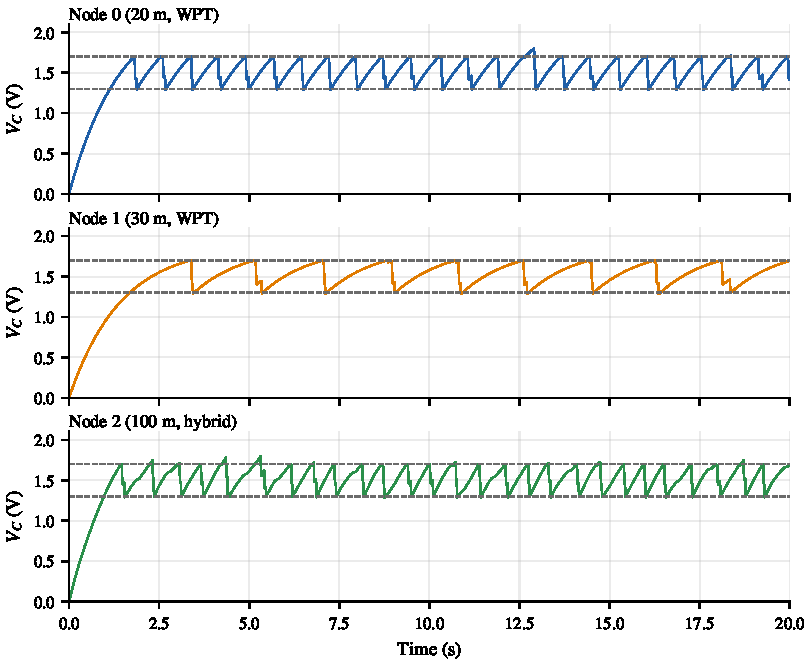
\includegraphics[width=0.92\linewidth]{fig_sawtooth}
\caption{Capacitor voltage of the three nodes of the broadcast demo (measured; random seed fixed for the figure). Node~0 and Node~1 harvest only from the base station's carrier at \SI{20}{m} and \SI{30}{m}. Node~2 is \SI{100}{m} away, too far to power itself from RF alone, and runs on its \emph{solar} trace instead. Dashed lines: $\Vhigh=\SI{1.7}{V}$ and $\Vlow=\SI{1.3}{V}$.}
\label{fig:sawtooth}
\end{figure}

\begin{enumerate}
 \item \textbf{Charging.} All capacitors start empty. Each rises along an RC
   curve towards the equivalent source voltage determined by the harvested
   power. The closer node reaches $\Vhigh=\SI{1.7}{V}$ sooner (about
   \SI{1.8}{s} for Node~0, about \SI{3.4}{s} for Node~1).
 \item \textbf{Activation.} Once $V\ge\Vhigh$ (and a random start-up delay of
   up to two seconds has elapsed), the node becomes \emph{active} and starts its
   duty cycle.
 \item \textbf{Duty-cycling.} Each time the node backscatters a packet it pays a
   large current for a few milliseconds---the sharp downward steps. Between
   packets it charges again---the slanted ramps.
 \item \textbf{Shut-down.} When the voltage falls to $\Vlow=\SI{1.3}{V}$ the node
   switches off and charges back up. The \emph{saw-tooth} is the signature of
   threshold-driven intermittent operation.
\end{enumerate}
The three traces differ in a way the radio alone would not predict. Node~2 is the farthest yet charges the \emph{fastest}, because the simulator
lets it draw on an external (solar) source; it also sends the most packets.
In the demo's 20-second run Node~0, Node~1 and Node~2 sent about 46, 18 and 58
packets respectively (counts vary slightly between runs). \textbf{Communication range is not the same as energy range.}

\section{The four design principles}
\label{sec:principles}

The paper lists four principles. We restate each and say where it is
realised.

\begin{description}[leftmargin=0.5cm,font=\sffamily\bfseries\color{ablue}]
 \item[Physically grounded modelling.] Energy dynamics are \emph{voltage- and
   current-based capacitor models} accounting for series resistance, leakage
   and simultaneous charging/discharging; RF propagation uses \emph{free-space
   path loss or the 3GPP TR~38.901 Urban Macro (UMa) model} with sectored
   antenna patterns; link budgets use the \emph{Friis transmission equation}
   with configurable gains, carrier frequency and medium attenuation.
   (Chapters~\ref{ch:pathloss}, \ref{ch:capacitor}.)
 \item[Modularity.] Capacitor, controller, backscatter model and base station are
   independent classes with defined interfaces, so each can be swapped without
   touching the framework. (Chapter~\ref{ch:architecture}.)
 \item[Energy awareness.] ``All simulated events are conditioned on the node's
   instantaneous energy state.'' The simulator tracks capacitor voltage at
   millisecond resolution, and models current consumption separately for the
   states \emph{listening, sensing, processing, transmitting}.
   (Chapter~\ref{ch:controller}.)
 \item[Scalability.] Built on SimPy with a $\SI{1}{ms}$ time step and
   interrupt-driven communication between node and base-station processes.
   Because nodes and base stations are stationary, coverage maps and link
   budgets are \emph{pre-computed once}, enabling ``hundreds of nodes''.
   (Chapter~\ref{ch:des}.)
\end{description}

\section{Time scales}

A system that couples electronics with protocols spans several orders of
magnitude in time. Keeping them straight prevents many modelling errors.

\begin{center}
\small
\renewcommand{\arraystretch}{1.15}
\begin{tabularx}{\linewidth}{@{}>{\sffamily\bfseries}p{4.3cm}lX@{}}
\toprule
Process & Time scale & Where it comes from\\
\midrule
Simulation tick & \SI{1}{ms} & \code{dt}, controller loop\\
Command / reply slot & \SIrange{5}{15}{ms} & BS schedule (demos)\\
Node transmit state & \SI{15}{ms} & \codew{DurationsMs.transmitting}\\
Capacitor charge time constant & $\tau_c=\Rs C=\SI{1.5}{s}$ & demo values\\
Time to first activation & $\sim$\SIrange{1.5}{3.5}{s} & Chapter~\ref{ch:capacitor}\\
Capacitor leakage constant & $\tau_\ell=\Rl C=\SI{30}{s}$ & demo values\\
Solar trace length & \SI{3}{s}, looped & \codew{EnvEnergySource}\\
Typical simulated horizon & \SIrange{15}{20}{s} & demos\\
\bottomrule
\end{tabularx}
\end{center}

\section{One poll, end to end}
\label{sec:walkthrough}

To prepare for Part~V, here is the complete story of one \emph{unicast
poll} in the shipped \code{unicast} demo, told in ten steps. Do not worry about
unfamiliar names yet: each is explained in its own chapter.
\begin{enumerate}[label=\textbf{\arabic*.}]
 \item At the start of its \emph{TX slot} the base station
   calls \codew{_deliver_command("send_data", target=0)}. It also looks ahead in its
   schedule to find the next RX slot(s) and attaches them to the command.
 \item The target node's \codew{BackscatterModule} checks that the \emph{downlink power}
   reaching the node exceeds its sensitivity. If not, the command is ignored. Otherwise
   it records the command and remembers the advertised slot.
 \item Meanwhile the node's \code{Controller}, which wakes up every millisecond,
   has been walking through its state machine. If the capacitor is above
   $\Vlow$ the node is \emph{active}.
 \item If the node is active and in its \emph{wait\_slot} state, the controller asks
   \codew{controller_tx_ready}: ``is a command pending, is $t$ inside the advertised
   slot, and is the slot not stale?''
 \item If all checks pass, the module calls \code{do_transmit}: it finds the
   best receiving sector of every base station, writes the payload and the
   pre-computed uplink RSSI into the base station object, and \emph{interrupts} the
   base station process.
 \item The base station is inside an RX window; the interrupt makes it append
   the packet to a \emph{buffer}.
 \item At the end of the window the base station groups buffered packets by
   subcarrier and time, applies the SINR/SIC rules, drops anything below its
   sector sensitivity, and logs the survivors as \code{RxPacket}s.
 \item The node meanwhile enters its \emph{transmitting} state: for
   \SI{15}{ms} the controller commands a \SI{5}{mA} load, and the capacitor
   voltage steps down by about \SI{0.25}{V}.
 \item The controller returns to \emph{listening}, then \emph{sensing} and
   \emph{processing}, and again waits for a slot. If the voltage has fallen to
   $\Vlow$, the node powers down instead and the capacitor recharges.
 \item The simulation continues, recording counters from which DER and
   throughput are computed (Chapter~\ref{ch:analysis}).
\end{enumerate}
Notice that \textbf{energy gates \emph{transmission}} (steps 3--4: a node that is
off or in the wrong state cannot answer), while the \textbf{radio gates
\emph{reception}} (step 2: a weak command is ignored). This asymmetry will matter in Chapter~\ref{ch:limits}.

\section{What is simulated and what is abstracted}

\begin{center}
\small
\renewcommand{\arraystretch}{1.15}
\begin{tabularx}{\linewidth}{@{}>{\sffamily\bfseries}p{3.1cm}XX@{}}
\toprule
Layer & Modelled explicitly & Abstracted away\\
\midrule
Propagation & Deterministic path loss (FSPL or 3GPP UMa), antenna patterns, two-way backscatter budget & Fading, shadowing, multipath, mobility\\
Physical layer & RSSI thresholds, SINR for collisions, thermal noise & Waveforms, modulation, coding, bit errors, synchronisation\\
Energy & Capacitor ODE (charge, leak, load), thresholds, per-state currents & Rectifier non-linearity (RF--DC efficiency), converter losses\\
MAC / protocol & Commands, slots, registration, polling, collisions, SIC & Preambles, CRCs, retransmission timers (user-defined)\\
Time & Millisecond clock, per-state durations & Anything below \SI{1}{ms}\\
\bottomrule
\end{tabularx}
\end{center}

\section{Map of the book to the code}
\label{sec:map}

Figure~\ref{fig:modulemap} shows the eight modules of the \code{amber} package
and how they depend on each other. The table below tells you where each theme
of this book is implemented and discussed.

\begin{center}
\small
\renewcommand{\arraystretch}{1.12}
\begin{tabularx}{\linewidth}{@{}>{\ttfamily}p{2.9cm}Xl@{}}
\toprule
\normalfont\sffamily\bfseries Module & Theory it implements & Chapters\\
\midrule
radiodevices & node, sector and base-station parameters & \ref{ch:coverage}\\
propagation & dB arithmetic, antenna patterns, Friis/UMa path loss, two-way backscatter budget, harvesting modes & \ref{ch:decibels}--\ref{ch:backscatter}, \ref{ch:harvest}, \ref{ch:coverage}\\
capacitor & RC charging, leakage, constant-current discharge & \ref{ch:capacitor}\\
energy & external (solar) energy trace & \ref{ch:harvest}\\
controller & threshold hysteresis and the duty-cycle state machine & \ref{ch:capacitor}, \ref{ch:controller}\\
backscatter & node-side protocol: registration, polling, slot validation & \ref{ch:protocols}, \ref{ch:bsmodule}\\
bsengine & schedules, RX windows, collisions, SIC & \ref{ch:aloha}--\ref{ch:sic}, \ref{ch:bsengine}\\
packet\_analysis & thermal noise, SINR, SIC, DER and throughput & \ref{ch:sic}, \ref{ch:analysis}\\
\bottomrule
\end{tabularx}
\end{center}

\begin{figure}[t]
\centering
\begin{tikzpicture}[node distance=0.55cm and 0.8cm]
 \node[mod] (rd) {\code{radiodevices}\\\scriptsize Node, Sector, BaseStation};
 \node[mod,right=of rd] (pr) {\code{propagation}\\\scriptsize path loss, antennas,\\\scriptsize CoverageMap};
 \node[mod,right=of pr] (pa) {\code{packet_analysis}\\\scriptsize noise, SIC, metrics};
 \node[mod,below=of rd] (cap) {\code{capacitor}\\\scriptsize $C$, $\Rs$, $\Rl$};
 \node[mod,below=of pr] (ctl) {\code{controller}\\\scriptsize voltage FSM};
 \node[mod,below=of pa] (bse) {\code{bsengine}\\\scriptsize schedule, RX, SIC};
 \node[mod,below=of cap] (en) {\code{energy}\\\scriptsize solar trace};
 \node[mod,below=of ctl] (bk) {\code{backscatter}\\\scriptsize node protocol};
 \draw[->] (pr) -- (rd);
 \draw[->] (pa) -- (pr);
 \draw[->] (ctl) -- (pr);
 \draw[->] (bse) -- (pa);
 \draw[->,dashed] (ctl) -- (cap);
 \draw[->,dashed] (ctl) -- (bk);
 \draw[->,dashed] (bk) -- (bse);
 \draw[->,dashed] (bse) -- (bk);
 \draw[->,dashed] (en) -- (pr);
\end{tikzpicture}
\caption{Module map. Solid arrows: Python imports. Dashed arrows: run-time interaction through SimPy interrupts and shared attributes (Chapter~\ref{ch:architecture}).}
\label{fig:modulemap}
\end{figure}

\section{Chapter summary}
\begin{itemize}
 \item Amber simulates nodes, base stations and the links between them; links are pre-computed because everything is stationary.
 \item A node's life is an RC charge, a threshold-triggered activation, a duty cycle of listen--sense--process--wait--transmit, and a shut-down at $\Vlow$.
 \item Energy gates a node's \emph{transmissions}; radio power gates its \emph{receptions}.
 \item The four principles (physical grounding, modularity, energy awareness, scalability) map onto Chapters~\ref{ch:pathloss}--\ref{ch:capacitor}, \ref{ch:architecture}, \ref{ch:controller} and \ref{ch:des}.
\end{itemize}

\section*{Exercises}
\begin{exercise}
Name the three entity types, and for each list two parameters that describe it (according to the paper).
\end{exercise}
\begin{exercise}
In Figure~\ref{fig:sawtooth}, Node~2 is farthest from the base station but activates first and sends the most packets. Give two possible explanations that do \emph{not} involve the quality of its radio link, and say which of the two the demo configuration actually implements.
\end{exercise}
\begin{exercise}
In the walk-through of Section~\ref{sec:walkthrough}, suppose that when the command arrives the node is in its \emph{processing} state and the advertised RX slot lasts \SI{10}{ms}. Under what condition can the node still reply in this slot?
\end{exercise}

\part{The Physics of Radio and Energy}

\chapter{Decibels, Noise and the Link Budget}
\label{ch:decibels}

\begin{defbox}[In this chapter you will learn]
\begin{itemize}
 \item why radio engineers work in decibels, and how to convert fluently between dB, dBm, dBi and linear units;
 \item how to write down a \emph{link budget} as a column of additions and subtractions;
 \item where thermal noise comes from, how to compute the noise floor of a receiver, and the difference between SNR, SINR and \emph{sensitivity};
 \item why the signal a backscatter receiver wants to detect is almost $\SI{100}{dB}$ weaker than the carrier that produced it.
\end{itemize}
\end{defbox}

Every number you will meet in Amber's propagation code is a power, a gain or a
loss. Before we study how they arise (Chapters~\ref{ch:antennas}--\ref{ch:backscatter}),
we need a common language for talking about them.

\section{Why a logarithmic scale?}

The powers in a link-budget differ by absurd factors. A base station sector
may radiate $\SI{46}{dBm}\approx\SI{40}{W}$; a backscattered reply may arrive at
the same base station with $\SI{-69}{dBm}\approx\SI{0.14}{nW}$. The ratio is
about $3\times10^{11}$. Worse, every stage between transmitter and receiver
\emph{multiplies} the power by a gain or loss factor: antenna gain, path loss,
power split, receiver gain. Working with products of numbers like $10^{-7}$
invites mistakes. Logarithms turn products into sums and make huge ratios fit
into small numbers.

\begin{defbox}[Decibel]
For two powers $P_1$ and $P_2$ the \emph{ratio in decibels} is
\[
 \left(\frac{P_2}{P_1}\right)_{\mathrm{dB}} = 10\log_{10}\frac{P_2}{P_1}.
\]
For an amplitude (voltage, field) ratio, $20\log_{10}$ is used instead, because
power is proportional to amplitude squared. A decibel value is always a
\emph{ratio}; an absolute power needs a reference.
\end{defbox}

The references we need:
\begin{itemize}
 \item \textbf{dBm}: reference $\SI{1}{mW}$. $\Pdbm = 10\log_{10}(P/\SI{1}{mW})$.
 \item \textbf{dBW}: reference $\SI{1}{W}$; $\Pdbm = P_{\mathrm{dBW}}+30$.
 \item \textbf{dBi}: antenna gain relative to an \emph{isotropic} radiator
   (Chapter~\ref{ch:antennas}).
\end{itemize}

\subsection{The conversion Amber uses}

Amber's three conversion helpers in \file{propagation.py} are one-liners:
\begin{align}
 P_{\mathrm{W}} &= 10^{(\Pdbm-30)/10}, && \text{\codew{dbm_to_watts}}\\
 \Pdbm &= 10\log_{10}\!\big(\max(P_{\mathrm{W}},10^{-15})\big)+30, && \text{\codew{watts_to_dbm}}\\
 G &= 10^{G_{\mathrm{dBi}}/10}. && \text{\codew{lin_from_dbi}}
\end{align}
The ``$-30$'' converts watts to milliwatts: $\SI{1}{W}=\SI{1000}{mW}=30$~dB
above one milliwatt. Notice the floor $10^{-15}\,\mathrm{W}=\SI{-120}{dBm}$ in
\codew{watts_to_dbm}: it prevents $\log_{10}0$, but it also means that
Amber cannot represent any power below $\SI{-120}{dBm}$ (a \emph{power of zero}
is reported as $\SI{-120}{dBm}$).

\begin{center}
\small
\renewcommand{\arraystretch}{1.1}
\begin{tabular}{@{}rrl@{\qquad}rrl@{}}
\toprule
dBm & Watts & Where it appears & dBm & Watts & Where it appears\\
\midrule
 46 & \SI{39.8}{W} & demo sector power & $-30$ & \SI{1}{\micro W} & weak energy harvest\\
 43 & \SI{20}{W} & \codew{Sector.power} default & $-45.7$ & \SI{27}{nW} & Node~0 uplink RSSI (demo)\\
 30 & \SI{1}{W} & paper's BS power & $-60$ & \SI{1}{nW} & \\
  0 & \SI{1}{mW} & Node~0 downlink (demo) & $-88$ & \SI{1.6}{pW} & thermal noise, \SI{100}{MHz}\\
$-10$ & \SI{100}{\micro W} & Node~2 downlink (demo) & $-100$ & \SI{0.1}{pW} & sector sensitivity\\
$-20$ & \SI{10}{\micro W} & & $-120$ & \SI{1}{fW} & Amber's representation floor\\
\bottomrule
\end{tabular}
\end{center}

\subsection{Rules of thumb you should memorise}

\begin{center}
\small
\begin{tabular}{@{}rl@{\qquad\qquad}rl@{}}
\toprule
$+3$ dB & $\approx\times2$ in power & $+10$ dB & $=\times10$\\
$-3$ dB & $\approx\times\tfrac12$ & $+20$ dB & $=\times100$\\
$+6$ dB & $\approx\times4$ & $+30$ dB & $=\times1000$\\
$0$ dBm & $=\SI{1}{mW}$ & $30$ dBm & $=\SI{1}{W}$\\
\bottomrule
\end{tabular}
\end{center}

\begin{reality}[Never add dBm values]
Gains and losses \emph{add} in decibels, but \emph{powers} add only in the
linear domain. Two interferers at $\SI{-70}{dBm}$ and $\SI{-73}{dBm}$ do not
produce $\SI{-143}{dBm}$ (that would be a \emph{product}, not a sum); they
produce
\[
 10\log_{10}\!\big(10^{-7}+10^{-7.3}\big)\ \mathrm{dBm}\;=\;\SI{-68.2}{dBm}.
\]
Amber follows this rule: \codew{compute_point_to_bs} converts each node's
power to watts, sums, and converts back to obtain \codew{total_pw_dbm}, and
\code{apply_sic} converts every power to watts before summing interference.
\end{reality}

\section{The link budget}
\label{sec:linkbudget}

A \emph{link budget} is the accounting that carries power from a transmitter to a
receiver. In decibels it is a simple column of additions:
\begin{equation}
 P_{\mathrm{rx}}\,[\mathrm{dBm}] \;=\; P_{\mathrm{tx}}\,[\mathrm{dBm}] \;+\; G_{\mathrm{tx}}\,[\mathrm{dBi}] \;-\; \mathrm{PL}\,[\mathrm{dB}] \;+\; G_{\mathrm{rx}}\,[\mathrm{dBi}]
 \;-\; L_{\mathrm{other}}\,[\mathrm{dB}].
\label{eq:linkbudget}
\end{equation}
In Amber $L_{\mathrm{other}}$ is the optional \emph{medium attenuation} term (Chapter~\ref{ch:pathloss}); everything
else maps one-to-one onto the arguments of \codew{compute_rx_power_watts}.
Link-budget thinking is the single most useful habit for understanding any
Amber output.

\begin{example}[The demo's downlink and uplink, line by line]
Consider \textbf{Node~0} of the shipped demos: it stands $\SI{20}{m}$ due north of the
base station, whose north-facing sector has $P_{\mathrm{tx}}=\SI{46}{dBm}$,
$G_{\max}=\SI{15}{dBi}$; the node antenna is \SI{0}{dBi}; carrier $\SI{924}{MHz}$; 3GPP UMa
LOS path loss gives $\mathrm{PL}=\SI{60.08}{dB}$ (Chapter~\ref{ch:pathloss}); the node
reflects a fraction $\eta=0.7$ ($-1.55$~dB).
\begin{center}
\renewcommand{\arraystretch}{1.1}
\begin{tabular}{@{}lrr@{}}
\toprule
\multicolumn{3}{@{}l}{\textbf{Downlink} (carrier to node)}\\
\midrule
Sector transmit power & +46.00 & dBm\\
Sector gain toward node (on boresight) & +15.00 & dBi\\
Path loss & $-60.08$ & dB\\
Node antenna gain & $+0.00$ & dBi\\
\midrule
\textbf{Power arriving at node} $P_{\mathrm{dl}}$ & \textbf{+0.92} & \textbf{dBm}\ ($\SI{1.24}{mW}$)\\
\midrule
\multicolumn{3}{@{}l}{\textbf{Backscatter uplink}}\\
\midrule
Reflected fraction $10\log_{10}0.7$ & $-1.55$ & dB\\
Node antenna gain (re-radiating) & $+0.00$ & dBi\\
Path loss (same distance, same model) & $-60.08$ & dB\\
Sector gain toward node (receiving) & $+15.00$ & dBi\\
\midrule
\textbf{Power arriving at base station} $P_{\mathrm{ul}}$ & \textbf{$-45.71$} & \textbf{dBm}\\
\bottomrule
\end{tabular}
\end{center}
The value $-45.71$ is exactly what the simulator logs in
\file{broadcast/output/rx_packets.csv} (column \code{rssi_dbm}) for Node~0.
Repeating the arithmetic for Node~1 ($\SI{30}{m}$, $\mathrm{PL}=\SI{62.10}{dB}$) gives
$-1.10$ and $-49.74$~dBm, and for Node~2 ($\SI{100}{m}$, $\mathrm{PL}=\SI{71.57}{dB}$) gives $-10.57$ and $-68.69$~dBm,
again matching the simulator. Notice that the uplink budget contains the
path loss \emph{twice}: this is the signature of backscatter.
\end{example}

\section{Thermal noise}
\label{sec:noise}

Every conductor above absolute zero carries random thermal motion of charge
carriers; a receiver sees it as noise. The available thermal-noise power in a
bandwidth $B$ is
\begin{equation}
 N_{\mathrm{th}} = k_B T B,\qquad k_B=\SI{1.38e-23}{J/K}.
\end{equation}
At the conventional reference temperature $T_0=\SI{290}{K}$,
$k_BT_0 = \SI{4.0e-21}{W/Hz}$, i.e.
\[
 10\log_{10}\!\frac{4.0\times10^{-21}\,\mathrm{W/Hz}}{10^{-3}\,\mathrm{W}} = \SI{-174}{dBm/Hz}.
\]
A real receiver adds noise of its own, summarised by the \emph{noise figure} $F$
(a ratio $\ge1$; $\mathrm{NF}=10\log_{10}F$): the receiver output has
$F$ times more noise than an ideal noiseless receiver would have. Hence
\begin{equation}
 N \;=\; k_B T_0 B F,\qquad N_{\mathrm{dBm}} = -174 + 10\log_{10}B_{\mathrm{Hz}} + \mathrm{NF}.
\label{eq:noise}
\end{equation}
This is exactly Amber's \codew{thermal_noise_watts(bandwidth_hz, noise_figure_db)},
with $T_0=\SI{290}{K}$ hard-coded and the paper's defaults $B=\SI{100}{MHz}$,
$\mathrm{NF}=\SI{6}{dB}$:
\[
 N_{\mathrm{dBm}} = -174+80+6=\SI{-88}{dBm}\quad(1.59\times10^{-12}\,\mathrm{W}).
\]

\section{SNR, SINR and sensitivity}
\label{sec:sinr}

Whether a receiver can decode a packet depends on how large the wanted signal
$P_s$ is compared with everything else.
\begin{defbox}[SNR, SINR]
\[
 \mathrm{SNR}=\frac{P_s}{N},\qquad
 \mathrm{SINR}\;\gamma=\frac{P_s}{\sum_{j\neq s}P_j+N},
\]
where the sum runs over \emph{interfering} signals (other nodes' backscatter in
Amber). Decoding is assumed to succeed when $\gamma\ge\gamma_{\mathrm{req}}$, a threshold determined
by modulation and coding.
\end{defbox}
A related but distinct concept is \emph{sensitivity}: the weakest received power
at which a receiver can still operate. In a classical receiver
$S_{\min}=N+\gamma_{\mathrm{req}}$ (plus implementation losses), so sensitivity
and noise floor are tied together by the bandwidth. \textbf{Amber stores sensitivity as an
independent threshold}:
\begin{itemize}
 \item \codew{Node.sensitivity_dbm} (default $\SI{-45}{dBm}$): the weakest downlink command a node notices;
 \item \codew{Sector.sensitivity_dbm} (default $\SI{-100}{dBm}$): the weakest backscatter packet a base-station sector can log.
\end{itemize}

\begin{reality}[Sensitivity and noise are not tied together in Amber]
With the default $B=\SI{100}{MHz}$, the noise floor is $\SI{-88}{dBm}$, \emph{above}
the default sector sensitivity of $\SI{-100}{dBm}$. A classical receiver could never
decode a packet at $\SI{-100}{dBm}$ in $\SI{100}{MHz}$ of noise (its SNR would be
$-12$~dB). For the two numbers to be consistent with $\gamma_{\mathrm{req}}=\SI{3}{dB}$ the noise bandwidth would have to be
about $\SI{3.2}{MHz}$ (Exercise~\ref{ex:bwsens}). In the simulator the two thresholds act at different
places:
\begin{itemize}
 \item the \emph{sensitivity} gate drops any packet whose RSSI is below the
   sector's value;
 \item the \emph{noise} enters only the SINR computation for \emph{colliding}
   packets (Chapter~\ref{ch:sic}). A \emph{lone} packet that passes the sensitivity
   gate is decoded no matter what its SNR is.
\end{itemize}
We verified the last point by injecting a single packet at $\SI{-105}{dBm}$
(SNR $=-17$~dB) into a base station with $\SI{-110}{dBm}$ sensitivity; it was logged as decoded.
When you use Amber, set \codew{bandwidth_hz} and the sensitivities consistently with each other.
\end{reality}

\section{The dynamic-range problem of backscatter}
\label{sec:dynrange}

Look again at the Node~0 budget: the base station \emph{transmits} $+46$~dBm per sector
and \emph{wants to receive} $-45.7$~dBm; for the farthest demo node the wanted signal
is $-68.7$~dBm. Between the transmitted carrier and the wanted backscatter lie
$92$--$115$~dB. A circulator or two separate antennas typically gives
only of order $20$--$30$~dB of isolation between transmit and receive paths, so
even the paper's $\SI{+30}{dBm}$ carrier leaks into the receiver at roughly
$0$ to $+10$~dBm---about $50$~dB \emph{stronger} than the strongest backscatter reply
in our demos. This
\emph{self-interference} is the central practical difficulty of backscatter
readers, and it is the reason the PRDCH structure and the \emph{subcarrier
shifting} of Chapter~\ref{ch:backscatter} exist: they move the reply into a
frequency region where the carrier is not.

\begin{codemap}
\small
\begin{tabularx}{\linewidth}{@{}>{\ttfamily}p{4.4cm}X@{}}
\toprule
\normalfont\bfseries Concept & \normalfont\bfseries Code (\file{amber/})\\
\midrule
dBm $\leftrightarrow$ W, dBi $\to$ linear & \codew{propagation.dbm_to_watts}, \codew{watts_to_dbm}, \codew{lin_from_dbi}\\
Link budget, Eq.~\eqref{eq:linkbudget} & \codew{propagation.compute_rx_power_watts}\\
Noise power, Eq.~\eqref{eq:noise} & \codew{packet_analysis.thermal_noise_watts}\\
SINR & \codew{packet_analysis.apply_sic}\\
Sensitivity gates & \codew{backscatter.receive_command} (node), \codew{bsengine._process_rx_buffer} (sector)\\
\bottomrule
\end{tabularx}
\end{codemap}

\section{Chapter summary}
\begin{itemize}
 \item Decibels turn the multiplicative chain of gains and losses into a sum; powers in dBm must be converted to linear before being added.
 \item A link budget $P_{\mathrm{rx}}=P_{\mathrm{tx}}+G_{\mathrm{tx}}-\mathrm{PL}+G_{\mathrm{rx}}$ explains every RSSI in Amber's output; we reproduced the demo's $-45.71$ and $-68.69$~dBm by hand.
 \item Noise is $N=k_BT_0BF$, giving $\SI{-88}{dBm}$ for $\SI{100}{MHz}$ and $\mathrm{NF}=\SI{6}{dB}$.
 \item Sensitivity is a configured threshold in Amber, \emph{decoupled} from the noise floor; noise matters only in collisions.
 \item Backscatter receivers face $\sim\SI{100}{dB}$ between carrier and wanted signal.
\end{itemize}

\section*{Exercises}
\begin{exercise}
Convert: (a) $\SI{33}{dBm}$ to watts; (b) $\SI{2}{\micro W}$ to dBm; (c) $\SI{-97}{dBm}$ to watts.
\end{exercise}
\begin{exercise}
Two co-channel interferers arrive at $-70$ and $\SI{-73}{dBm}$. What is their combined power in dBm? What would it be if there were four equal interferers at $\SI{-73}{dBm}$?
\end{exercise}
\begin{exercise}
Compute the thermal noise floor in dBm for $B=\SI{1}{MHz}$ and $\mathrm{NF}=\SI{8}{dB}$, and for $B=\SI{100}{MHz}$ and $\mathrm{NF}=\SI{6}{dB}$. By how many dB do they differ?
\end{exercise}
\begin{exercise}\label{ex:linkbudget1}
A sector transmits $\SI{30}{dBm}$ with $\SI{17}{dBi}$ toward a node with a $\SI{1}{dBi}$ antenna, over a path loss of $\SI{80}{dB}$. (a) What is the downlink power at the node in dBm and in $\si{\micro W}$? (b) Does it exceed Amber's default node sensitivity of $\SI{-45}{dBm}$? (c) If the node reflects $\eta=0.5$ and the return path has the same loss and the same sector gain toward the node, what uplink power arrives at the base station?
\end{exercise}
\begin{exercise}\label{ex:bwsens}
Show that a receiver with noise figure $\SI{6}{dB}$ has a $\SI{-100}{dBm}$ sensitivity at $\gamma_{\mathrm{req}}=\SI{3}{dB}$ only if its noise bandwidth is about $\SI{3.2}{MHz}$.
\end{exercise}

\chapter{Antennas, Sectors and Geometry}
\label{ch:antennas}

\begin{defbox}[In this chapter you will learn]
\begin{itemize}
 \item what antenna \emph{gain} really means and why it is measured in dBi;
 \item the 3GPP TR~38.901 horizontal sector pattern, including its half-power and floor behaviour;
 \item the geometric bookkeeping Amber performs: compass versus mathematical angles, bearings and angular error;
 \item how a three-sector base station divides the plane and how a node's ``best'' sector is chosen.
\end{itemize}
\end{defbox}

\section{Gain: concentrating a fixed amount of power}
\label{sec:gain}

An \emph{isotropic} radiator spreads power equally in all directions; its power
density at distance $d$ is $P_t/(4\pi d^2)$. No physical antenna is isotropic,
and the laws of energy conservation say that an antenna cannot create power, only
\emph{redistribute} it. A \emph{directional} antenna concentrates power into some
directions at the expense of others. Its \emph{gain} $G(\theta,\varphi)$ in a
direction is the ratio of the power density it produces there to that of an
isotropic radiator fed with the same power. We express it in \si{\dBi}.

\begin{intuition}[Gain as a flashlight]
Imagine pouring a fixed amount of light into a room. A bare bulb lights
everything dimly; a torch lights a narrow cone brightly and the rest not at all.
The brightness in the cone divided by the bare-bulb brightness is the gain. The
\emph{narrower} the beam, the \emph{higher} the gain---a fact we can quantify.
\end{intuition}

For a beam whose half-power widths are $\theta_{az}$ and $\theta_{el}$ (in
degrees) a standard approximation of the peak \emph{directivity} is
\begin{equation}
 D \;\approx\; \frac{41\,253}{\theta_{az}\,\theta_{el}},
\label{eq:directivity}
\end{equation}
because $41\,253\ \mathrm{deg}^2$ is the solid angle of the whole sphere in square
degrees. A cellular panel with a $65^\circ$ azimuth beamwidth and a vertical
beamwidth of roughly $10^\circ$ has $D\approx63\approx\SI{18}{dBi}$; losses
reduce this to the $\SI{15}{dBi}$--$\SI{17}{dBi}$ used in Amber's demos and in the
paper ($\SI{17}{dBi}$). A node's small antenna is nearly omnidirectional:
$\SI{0}{dBi}$ by default, $\SI{1}{dBi}$ in the paper's experiment.

\section{The 3GPP sector pattern}
\label{sec:patt3gpp}

Amber models a base-station sector with the \emph{horizontal} pattern of
3GPP TR~38.901 \citep{3gpp38901}. With $\varphi$ the angle between the target and the
antenna's boresight, $\varphi_{3\mathrm{dB}}$ the half-power beamwidth
(\codew{beamwidth_deg}) and $A_m$ the maximum attenuation (front-to-back
ratio), the attenuation below the peak is
\begin{equation}
 A_H(\varphi) \;=\; \min\!\left[\,12\left(\frac{\varphi}{\varphi_{3\mathrm{dB}}}\right)^{\!2},\; A_m\right]\ \mathrm{dB},
 \qquad
 G(\varphi) = G_{\max}-A_H(\varphi),
\label{eq:patt3gpp}
\end{equation}
with $A_m=\SI{30}{dB}$ as hard-wired in \codew{antenna_from_sector}.

\begin{figure}[t]
\centering
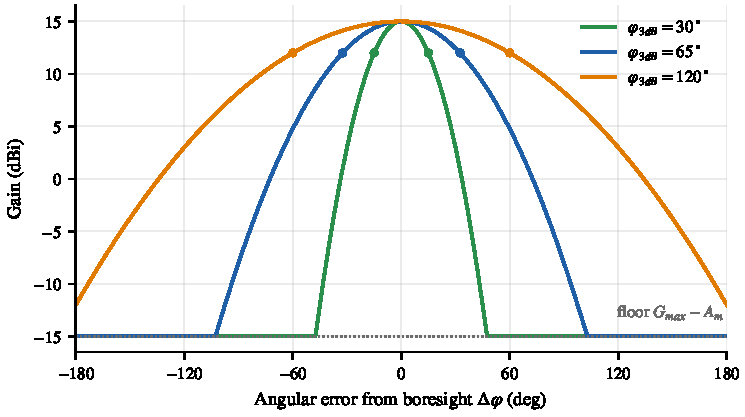
\includegraphics[width=0.85\linewidth]{fig_antenna}
\caption{The pattern of Eq.~\eqref{eq:patt3gpp} for $G_{\max}=\SI{15}{dBi}$ and three beamwidths. Dots mark the half-power points at $\pm\varphi_{3\mathrm{dB}}/2$ ($G_{\max}-\SI{3}{dB}$). Beyond about $1.58\,\varphi_{3\mathrm{dB}}$ the pattern is flat at $G_{\max}-A_m$.}
\label{fig:antenna}
\end{figure}

Three properties follow immediately and are worth internalising.
\begin{enumerate}
 \item \textbf{The half-power points.} At $\varphi=\varphi_{3\mathrm{dB}}/2$ the attenuation is
   $12\cdot\tfrac14=\SI{3}{dB}$. So $\varphi_{3\mathrm{dB}}$ is the \emph{full} width of the beam at
   half power---consistent with the name.
 \item \textbf{The floor.} The parabola reaches $A_m$ at
   $\varphi=\varphi_{3\mathrm{dB}}\sqrt{A_m/12}=1.58\,\varphi_{3\mathrm{dB}}$; for
   $65^\circ$ that is $102.8^\circ$. Beyond that the sector's gain is
   $G_{\max}-30$, i.e.\ $\SI{-15}{dBi}$ for a $\SI{15}{dBi}$ panel. The antenna
   never has a perfect null.
 \item \textbf{Narrow beams roll off fast.} A $30^\circ$ sector drops $\SI{12}{dB}$ at $\pm 30^\circ$,
   whereas a $65^\circ$ sector drops only about $\SI{2.6}{dB}$ there.
\end{enumerate}
We can check item~2 against the simulator. In the demo, \textbf{Node~0}
lies due north of the base station; the sectors at azimuths
$0^\circ,120^\circ,240^\circ$ see it at angular errors $0^\circ$, $120^\circ$ and
$120^\circ$. Sector~1 and~2 are therefore at the floor, $30$~dB below sector~0, and indeed
the simulator reports downlink powers of $+0.9$, $-29.1$ and $-29.1$~dBm for sectors
\code{BS0_S0}, \code{BS0_S1}, \code{BS0_S2}.

\begin{reality}[Only the azimuth cut is modelled]
The full 3GPP element pattern adds a \emph{vertical} term $A_V(\theta)$ and combines the two.
Amber implements the horizontal cut only (\codew{SectorAntenna3GPP.gain_linear}). The
base station's height enters path loss through the 3-D distance, but
\emph{there is no downtilt and no vertical attenuation}. For a node close to the mast
(a $\SI{20}{m}$ ground distance under a $\SI{25}{m}$ mast means the node is $\approx50^\circ$
below the horizon) a real panel would give less than the modelled gain.
\end{reality}

\section{Sectorisation}
\label{sec:sectorisation}

A cell site rarely uses a single omnidirectional antenna. The usual
arrangement is \emph{three sectors of $120^\circ$ spacing}, each with a
directional panel. This multiplies capacity (each sector reuses the spectrum)
and, for a given transmit power, lifts the gain in each served direction.

Because the sector pattern falls off by about $\SI{10}{dB}$ at the
crossover ($60^\circ$ off boresight when sectors are spaced $120^\circ$ apart),
a $65^\circ$ panel leaves a \emph{ripple} in the coverage:
\[
 G(60^\circ)=15-12\left(\tfrac{60}{65}\right)^{2}=\SI{4.8}{dBi},
\]
more than $\SI{10}{dB}$ below the peak. This ripple is visible as the darker
bands between sectors in coverage maps such as Figure~\ref{fig:covmap}.

\begin{figure}[t]
\centering
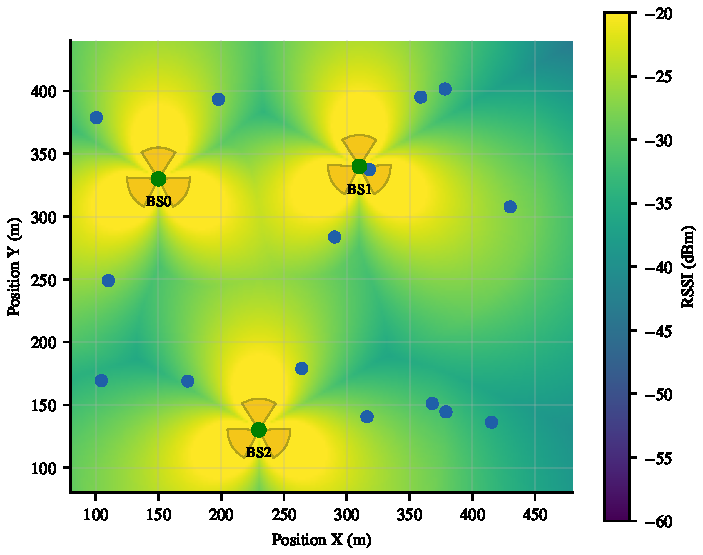
\includegraphics[width=0.6\linewidth]{fig_coverage}
\caption{A coverage map produced by Amber's \code{CoverageMap} for an illustrative deployment (three base stations of three $65^\circ$ sectors, $\SI{30}{dBm}$, $\SI{17}{dBi}$, $\SI{924}{MHz}$, 15 random nodes), in the style of the paper's Figure~1. Colour is the \emph{best} received power among all sectors (Chapter~\ref{ch:coverage}). This figure is our own example, not the paper's data.}
\label{fig:covmap}
\end{figure}

\paragraph{The best sector.}
Amber assigns each point (grid point or node) to the sector delivering the
highest power: the ``owner'' of that point (\code{owner}, \code{best_pw_dbm}). There is
no hysteresis or handover logic, and ties are resolved in favour of the sector
evaluated first (the comparison is a strict ``$>$'').

\section{Geometry: bearings and angular errors}
\label{sec:geometry}

To evaluate Eq.~\eqref{eq:patt3gpp} we need $\varphi$, the angle between a
sector's boresight and the direction to a node. Two angle conventions meet here, and
confusing them is a classic source of bugs.
\begin{itemize}
 \item \textbf{Compass} (navigation) azimuth: $0^\circ$ is North, increasing \emph{clockwise}.
   This is what \codew{Sector.azimuth_deg} and \codew{Node.azimuth_deg} use.
 \item \textbf{Mathematical} angle: $0^\circ$ is East, increasing \emph{counter-clockwise}.
   This is what \codew{numpy.arctan2} returns.
\end{itemize}
The conversion is $\theta_{\mathrm{math}}=(90^\circ-\alpha_{\mathrm{compass}})\bmod360^\circ$
(\codew{compass_to_math}). The bearing from a point $(x_0,y_0)$ to $(x,y)$ is
$\operatorname{atan2}(y-y_0,\,x-x_0)\bmod360^\circ$ (\code{bearing_deg}), and the
smallest angular difference between two angles, correct across the $0^\circ/360^\circ$ seam, is
\begin{equation}
 \Delta\varphi=\left|\,(\theta_{\mathrm{target}}-\theta_{\mathrm{bore}}+180^\circ)\bmod360^\circ-180^\circ\,\right|
\label{eq:angerr}
\end{equation}
(\codew{angular_error_deg}). The shift by $180^\circ$ followed by the modulus maps the
difference into $[-180^\circ,180^\circ)$, whose absolute value is the shortest
way round.

\begin{figure}[t]
\centering
\begin{tikzpicture}[scale=1.05]
 \fill[ablue!14] (0,0) -- (27.5:3.0) arc (27.5:92.5:3.0) -- cycle;
 \draw[->,agrey] (-1.2,0) -- (4.3,0) node[right,lab,align=left] {East\\math $0^\circ$};
 \draw[->,agrey] (0,-1.0) -- (0,3.6) node[above,lab,align=center] {North, compass $0^\circ$};
 \draw[->,very thick,ablue] (0,0) -- (60:3.4) node[above right,lab,align=left] {boresight\\compass $30^\circ$\\math $60^\circ$};
 \draw[->,thick,agreen] (0,0) -- (12:3.9) node[right,lab,align=left] {target bearing\\math $12^\circ$};
 \draw[ablue] (1.0,0) arc (0:60:1.0);
 \node[lab,ablue] at (1.35,0.35) {$\theta_{\mathrm{bore}}=60^\circ$};
 \draw[aorange] (0,1.6) arc (90:60:1.6);
 \node[lab,aorange,anchor=south west] at (0.35,1.7) {$\alpha=30^\circ$};
 \draw[ared,thick] (2.6,0.56) arc (12:60:2.65);
 \node[lab,ared,anchor=west] at (2.85,1.55) {$\Delta\varphi=48^\circ$};
\end{tikzpicture}
\caption{Compass versus mathematical angles. The sector's boresight points at compass azimuth $30^\circ$ (math $60^\circ$); a target at math bearing $12^\circ$ is $\Delta\varphi=48^\circ$ off boresight and sees the pattern attenuation $12(48/65)^2=\SI{6.5}{dB}$ for a $65^\circ$ sector.}
\label{fig:angles}
\end{figure}

\begin{example}[Why a node due north sees the $120^\circ$ sector at the floor]
The sector with compass azimuth $120^\circ$ has $\theta_{\mathrm{bore}}=(90-120)\bmod360=330^\circ$.
A node due north has math bearing $90^\circ$. By Eq.~\eqref{eq:angerr}:
$\left|(90-330+180)\bmod 360-180\right|=\left|300-180\right|=120^\circ$, and
$12(120/65)^2=40.9>A_m$, so the attenuation clips at $\SI{30}{dB}$.
\end{example}

\section{Node antennas and reciprocity}

A node is described by \codew{antenna_type}: ``omni'' (default; gain
\codew{antenna_gain_dbi}, independent of direction) or ``3GPP'' (the same pattern as a
sector, with the node's own \code{azimuth_deg} and \codew{beamwidth_deg}).
In both the downlink and the uplink the simulator evaluates the node's gain
toward the base station \emph{with the same function}. This reflects the
\emph{reciprocity} of passive antennas: the pattern is the same in transmit and
receive. For backscatter, where one antenna both receives the carrier and
re-radiates the reflection, reciprocity is physically exact.

\begin{codemap}
\small
\begin{tabularx}{\linewidth}{@{}>{\ttfamily}p{5.0cm}X@{}}
\toprule
\normalfont\bfseries Concept & \normalfont\bfseries Code (\file{amber/propagation.py})\\
\midrule
Pattern Eq.~\eqref{eq:patt3gpp} & \codew{SectorAntenna3GPP.gain_linear}\\
Omni antenna & \codew{OmniAntenna.gain_linear}\\
Build antenna from device & \codew{antenna_from_sector}, \codew{antenna_from_node}\\
Compass $\to$ math & \codew{compass_to_math}\\
Bearing, error Eq.~\eqref{eq:angerr} & \code{bearing_deg}, \codew{angular_error_deg}\\
Best sector & the \codew{mask = p_w > best_pw_w} update in \codew{compute_bs_to_point}\\
\bottomrule
\end{tabularx}
\end{codemap}

\section{Chapter summary}
\begin{itemize}
 \item Gain redistributes power; narrower beams have higher gain, $D\approx41\,253/(\theta_{az}\theta_{el})$.
 \item Amber uses 3GPP's horizontal pattern: $G=G_{\max}-\min[12(\varphi/\varphi_{3\mathrm{dB}})^2,30]$.
 \item Three $65^\circ$ sectors at $120^\circ$ spacing leave a $\approx10$~dB ripple at the crossovers.
 \item Compass and mathematical angles differ; Eq.~\eqref{eq:angerr} gives the correct shortest angular error.
 \item No vertical pattern or downtilt is modelled.
\end{itemize}

\section*{Exercises}
\begin{exercise}
A sector has $G_{\max}=\SI{17}{dBi}$ and $\varphi_{3\mathrm{dB}}=65^\circ$. What is its gain at an angular error of $40^\circ$? At $90^\circ$? At $150^\circ$?
\end{exercise}
\begin{exercise}
Find the angular error at which the pattern reaches its floor for (a) $\varphi_{3\mathrm{dB}}=30^\circ$ and (b) $\varphi_{3\mathrm{dB}}=120^\circ$.
\end{exercise}
\begin{exercise}
Convert the compass azimuths $0^\circ$, $45^\circ$, $135^\circ$, $270^\circ$ to mathematical angles. A sector has compass azimuth $10^\circ$; a node is at math bearing $350^\circ$. What is the angular error?
\end{exercise}
\begin{exercise}
Three sectors with $\varphi_{3\mathrm{dB}}=65^\circ$ at compass azimuths $0^\circ,120^\circ,240^\circ$. For a node at compass bearing $60^\circ$ from the mast, compute each sector's gain (take $G_{\max}=\SI{15}{dBi}$) and say which sector Amber would call the owner.
\end{exercise}
\begin{exercise}
Estimate the peak gain of a panel with a $90^\circ\times15^\circ$ beam using Eq.~\eqref{eq:directivity}.
\end{exercise}

\chapter{Path Loss: From Friis to 3GPP Urban Macro}
\label{ch:pathloss}

\begin{defbox}[In this chapter you will learn]
\begin{itemize}
 \item how the Friis transmission equation follows from two simple ideas---power density and effective aperture;
 \item why real environments need path-loss models beyond free space, and what the \emph{breakpoint distance} means;
 \item the 3GPP TR~38.901 Urban Macro (UMa) line-of-sight and non-line-of-sight formulas that Amber implements, with all constants explained;
 \item how Amber applies medium attenuation, and two subtle behaviours of the code near the base station.
\end{itemize}
\end{defbox}

\section{Free-space propagation: Friis}
\label{sec:friis}

Two ideas, both geometric, give the free-space law.

\paragraph{Idea 1: power density.}
An isotropic transmitter of power $P_t$ spreads its power over a sphere of
area $4\pi d^2$ at distance $d$. With antenna gain $G_t$ toward the receiver the power
density is
\[
 S \;=\; \frac{P_t\,G_t}{4\pi d^2}\qquad[\mathrm{W/m^2}].
\]

\paragraph{Idea 2: effective aperture.}
A receiving antenna of gain $G_r$ intercepts power from a passing wave as if it
had an \emph{effective area}
\[
 A_e \;=\; \frac{G_r\lambda^2}{4\pi},\qquad \lambda=\frac{c}{f_c}.
\]
This shows an interesting fact: at a given gain, a lower frequency means a larger
effective area, so a $\SI{924}{MHz}$ antenna ($\lambda=\SI{0.325}{m}$) captures
$\approx$10 times more power than a $\SI{3}{GHz}$ one of the same gain. Multiply the two:
\begin{equation}
 P_r \;=\; S\,A_e \;=\; P_t\,G_t\,G_r\left(\frac{\lambda}{4\pi d}\right)^{\!2}.
\label{eq:friis}
\end{equation}
This is the \emph{Friis transmission equation} \citep{friis1946}. The last factor,
\begin{equation}
 L_{\mathrm{FS}}(d)=\left(\frac{\lambda}{4\pi d}\right)^{2},\qquad
 \mathrm{PL}_{\mathrm{FS}}(d)=20\log_{10}\frac{4\pi d}{\lambda}\ \mathrm{dB},
\label{eq:fspl}
\end{equation}
is the \emph{free-space path loss}. It is exactly Amber's \code{fspl_lin}. In
convenient units, $\mathrm{PL}_{\mathrm{FS}}=32.45+20\log_{10}f_{\mathrm{MHz}}+20\log_{10}d_{\mathrm{km}}$.
At $\SI{924}{MHz}$ the loss at $\SI{1}{m}$ is $\SI{31.76}{dB}$, and every doubling of
distance costs $20\log_{10}2=\SI{6.02}{dB}$ more.

\begin{keyidea}[A common misconception]
Free-space ``loss'' is not absorption. No energy disappears; it simply
\emph{spreads out}. The $\lambda^2$ in the formula comes from the receive
aperture, not from the medium: path loss at a fixed distance grows with
frequency because the receiving antenna gets \emph{smaller}.
\end{keyidea}

\begin{example}[Free space at $\SI{20}{m}$]
$\lambda=3\times10^{8}/924\times10^{6}=\SI{0.3247}{m}$.
$\mathrm{PL}_{\mathrm{FS}}(20)=20\log_{10}(4\pi\cdot20/0.3247)=20\log_{10}(774)=\SI{57.78}{dB}$.
\end{example}

\section{Beyond free space}
\label{sec:beyondfs}

Free space is the best case. In a real street the wave also reflects from the ground and
buildings, is blocked by obstacles, and diffracts around edges. Empirically one
finds that received power falls as $d^{-n}$ with a \emph{path-loss exponent} $n$
ranging from about 2 (open) to 4--6 (cluttered). The simplest physical
mechanism that makes $n=4$ is the \emph{two-ray ground reflection}: the direct
ray and its reflection from the ground interfere destructively beyond a
\emph{breakpoint distance} $d_{BP}\approx4h_th_r/\lambda$ (for antenna heights $h_t,h_r$); inside it the
loss is nearly free-space ($n\approx2$) and outside it is steeper ($n\approx4$).
This ``two-slope'' behaviour is built into the 3GPP urban macro model.

\section{3GPP TR 38.901 Urban Macro (UMa)}
\label{sec:uma}

3GPP's channel-model report TR~38.901 \citep{3gpp38901} specifies a statistical
path-loss formula for every deployment scenario for carrier frequencies between
$0.5$ and $\SI{100}{GHz}$. Amber implements the \textbf{UMa} scenario in
\codew{urban_macro_loss_db_38_901}. Let $f_c$ be in GHz, $h_{BS}$ the
base-station height (default $\SI{25}{m}$) and $h_{UT}$ the node height
(default $\SI{1.5}{m}$). The code defines
\begin{align}
 d_{3D}&=\sqrt{d_{2D}^2+(h_{BS}-h_{UT})^2}\quad(\text{clamped to}\ge\SI{10}{m}),\\
 d'_{BP}&=\frac{4\,(h_{BS}-1)\,(h_{UT}-1)\,f_c}{c}\quad[f_c\ \text{in Hz in the code}],
\end{align}
where the ``$-1$'' is the effective environment height $h_E=\SI{1}{m}$. For
the demo's heights $d'_{BP}=4\cdot24\cdot0.5\cdot924\times10^{6}/3\times10^{8}=\SI{147.8}{m}$.

\paragraph{Line of sight (LOS).} The loss has two slopes:
\begin{align}
 \mathrm{PL}_1 &= 28.0+22\log_{10}d_{3D}+20\log_{10}f_c, && 10\,\mathrm{m}\le d_{2D}\le d'_{BP},\label{eq:pl1}\\
 \mathrm{PL}_2 &= 28.0+40\log_{10}d_{3D}+20\log_{10}f_c-9\log_{10}\!\big(d_{BP}'^{\,2}+(h_{BS}-h_{UT})^2\big), && d_{2D}> d'_{BP}.\label{eq:pl2}
\end{align}
Inside the breakpoint the exponent is $2.2$ (close to free space); outside it is
$4.0$. The last term of $\mathrm{PL}_2$ makes the curve continuous at $d'_{BP}$.

\paragraph{Non line of sight (NLOS).} The 3GPP formula is
\begin{equation}
 \mathrm{PL}'_{\mathrm{NLOS}}=13.54+39.08\log_{10}d_{3D}+20\log_{10}f_c-0.6\,(h_{UT}-1.5),
\end{equation}
and the model uses $\mathrm{PL}_{\mathrm{NLOS}}=\max\!\big(\mathrm{PL}_{\mathrm{LOS}},\,\mathrm{PL}'_{\mathrm{NLOS}}\big)$ so that NLOS is never better than LOS. The
code selects LOS or NLOS with the single flag \codew{CoverageMap.los}; there is no
probabilistic LOS/NLOS switching with distance.

\begin{figure}[t]
\centering
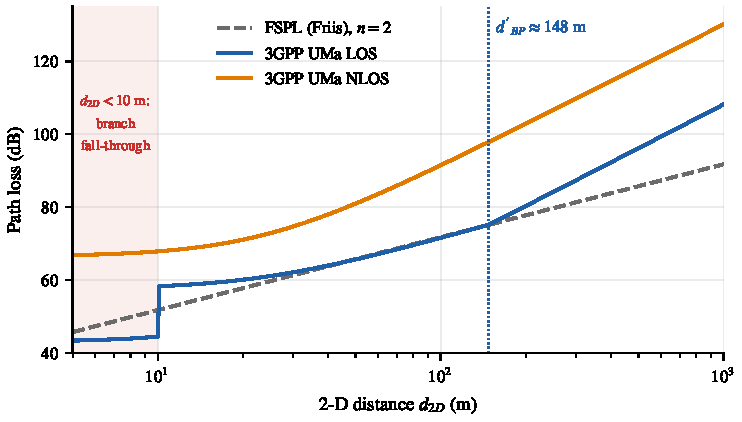
\includegraphics[width=0.85\linewidth]{fig_pathloss}
\caption{Path loss at $\SI{924}{MHz}$ with $h_{BS}=\SI{25}{m}$, $h_{UT}=\SI{1.5}{m}$, computed by Amber's own functions. Free space (dashed) and UMa LOS agree closely up to the breakpoint $d'_{BP}\approx\SI{148}{m}$, after which LOS steepens to a $40$~dB/decade slope. NLOS is $\approx11$--$22$~dB worse. The shaded region at left marks the code's non-physical behaviour below $\SI{10}{m}$ (see the reality check below).}
\label{fig:pathloss}
\end{figure}

\begin{center}
\small
\renewcommand{\arraystretch}{1.08}
\begin{tabular}{@{}rrrrr@{}}
\toprule
$d_{2D}$ (m) & $d_{3D}$ (m) & FSPL$(d_{2D})$ (dB) & UMa LOS (dB) & UMa NLOS (dB)\\
\midrule
 20 & 30.9 & 57.8 & 60.1 & 71.1\\
 30 & 38.1 & 61.3 & 62.1 & 74.6\\
 50 & 55.2 & 65.7 & 65.6 & 80.9\\
100 & 102.7 & 71.8 & 71.6 & 91.5\\
148 & 149.7 & 75.2 & 75.2 & 97.9\\
300 & 300.9 & 81.3 & 87.3 & 109.7\\
500 & 500.6 & 85.7 & 96.1 & 118.4\\
1000 & 1000.3 & 91.8 & 108.2 & 130.1\\
\bottomrule
\end{tabular}
\end{center}
\noindent\emph{Generated by calling Amber's \code{fspl_lin} and \codew{urban_macro_loss_db_38_901}.}

\begin{example}[Path loss at $\SI{100}{m}$ by hand]
$d_{3D}=\sqrt{100^2+23.5^2}=\SI{102.72}{m}$, below the breakpoint, so Eq.~\eqref{eq:pl1}:
$28+22\log_{10}102.72+20\log_{10}0.924=28+44.26-0.69=\SI{71.57}{dB}$, matching the
table and the downlink budget of the demo's Node~2 (Chapter~\ref{ch:decibels}).
\end{example}

\section{Medium attenuation}

\codew{compute_rx_power_watts} accepts an optional \codew{extra_np_per_m}, a
medium attenuation $\alpha$ in nepers per metre, and multiplies the received
power by $\e^{-\alpha d}$. Two remarks. First, in electromagnetics a ``neper
per metre'' usually quantifies attenuation of the field \emph{amplitude}
($\SI{8.686}{dB/m}$ per Np/m); because Amber applies the factor to
\emph{power}, its $\alpha$ corresponds to $4.343\,\alpha$~dB/m. Second, the
attenuation is applied once per hop, so a backscatter link suffers it \emph{twice}.
It is zero by default.

\section{What Amber assumes about the channel}

Everything in this chapter is a \emph{deterministic, static} function of
distance and angles. There is no small-scale fading (Rayleigh/Rician), no
log-normal shadow fading (3GPP specifies $\sigma_{SF}$ of several dB for UMa),
no multipath delay spread, no frequency selectivity and no
mobility. This is a conscious system-level simplification: it makes link budgets
computable \emph{once} (Chapter~\ref{ch:des}) and results repeatable, at the
price of not reproducing the variability of real channels.

\begin{reality}[Two behaviours of the path-loss code near the mast]
\textbf{(1) A $\SI{14}{dB}$ step at $\SI{10}{m}$.} The LOS formula selects
$\mathrm{PL}_1$ only for $10\le d_{2D}\le d'_{BP}$ (the range in which 3GPP defines
it). For $d_{2D}<\SI{10}{m}$ the code falls through to the \emph{post-breakpoint}
branch $\mathrm{PL}_2$. The result at $\SI{5}{m}$ is $\SI{43.4}{dB}$, whereas
$\mathrm{PL}_1$ would give $\SI{57.7}{dB}$; the curve jumps by $\SI{13.8}{dB}$ between
$\SI{9.99}{m}$ and $\SI{10}{m}$ (Figure~\ref{fig:pathloss}). We measured this directly.
Keep nodes at least $\SI{10}{m}$ (horizontally) from a mast. Note that the shipped custom-protocol demo
places nodes from $\SI{5}{m}$ outward, so a few of its nodes enjoy this extra $\sim\SI{14}{dB}$.

\textbf{(2) Free space uses the horizontal distance.} In
\codew{pathloss="fspl"} mode the function receives $d_{2D}$, not the slant range
$d_{3D}$: the $\SI{25}{m}$ mast height is ignored. At $d_{2D}=\SI{5}{m}$ this understates
the loss by $14$~dB; at $\SI{100}{m}$ by only $\SI{0.2}{dB}$. The UMa model does
use $d_{3D}$ internally.
\end{reality}

\begin{codemap}
\small
\begin{tabularx}{\linewidth}{@{}>{\ttfamily}p{5.2cm}X@{}}
\toprule
\normalfont\bfseries Concept & \normalfont\bfseries Code (\file{amber/propagation.py})\\
\midrule
Friis, Eq.~\eqref{eq:friis}, \eqref{eq:fspl} & \code{fspl_lin}, \codew{compute_rx_power_watts}\\
UMa LOS/NLOS & \codew{urban_macro_loss_db_38_901}\\
Model selection & \code{pathloss} string: \code{"fspl"} or \code{"macro"}/\code{"3gpp"}/\code{"urban"}\\
Medium attenuation & factor \codew{np.exp(-extra_np_per_m * distance_m)}\\
\bottomrule
\end{tabularx}
\end{codemap}

\section{Chapter summary}
\begin{itemize}
 \item Friis: $P_r=P_tG_tG_r(\lambda/4\pi d)^2$---spreading plus a $\lambda^2$ aperture; $\mathrm{PL}_{FS}(\SI{1}{m},\SI{924}{MHz})=\SI{31.76}{dB}$.
 \item UMa LOS has exponent $2.2$ before and $4.0$ after the breakpoint $d'_{BP}=4(h_{BS}-1)(h_{UT}-1)f_c/c$; NLOS is $\max(\text{LOS},\ \text{NLOS}')$.
 \item Amber's channel is deterministic and static: no fading or shadowing.
 \item Beware $d_{2D}<\SI{10}{m}$ (a $14$~dB discontinuity) and the horizontal-distance convention in FSPL mode.
\end{itemize}

\section*{Exercises}
\begin{exercise}
Derive Eq.~\eqref{eq:friis} from the two ideas of Section~\ref{sec:friis}, and then compute the free-space loss at $\SI{924}{MHz}$ and $\SI{3.5}{GHz}$ for $\SI{50}{m}$ with $G_r=G_t=1$. Why is the second larger?
\end{exercise}
\begin{exercise}
Compute $d'_{BP}$ for $h_{BS}=\SI{30}{m}$, $h_{UT}=\SI{2}{m}$ at $\SI{2}{GHz}$. Is a node at $d_{2D}=\SI{200}{m}$ before or after the breakpoint?
\end{exercise}
\begin{exercise}
Using Eq.~\eqref{eq:pl2}, compute the UMa LOS loss at $d_{2D}=\SI{300}{m}$ for the demo parameters ($\SI{924}{MHz}$, $25$/$\SI{1.5}{m}$). Compare with the table.
\end{exercise}
\begin{exercise}
A medium attenuation of $\alpha=0.01$~Np/m is configured. What is the extra loss in dB per hop at $\SI{100}{m}$ as Amber applies it? And over the round trip of a backscatter link?
\end{exercise}
\begin{exercise}
By what factor (in dB) does the \emph{uplink} power at the base station change when a node moves from $\SI{50}{m}$ to $\SI{100}{m}$ in the LOS regime below the breakpoint, compared with the change of the \emph{downlink} power at the node?
\end{exercise}

\chapter{Backscatter Communication}
\label{ch:backscatter}

\begin{defbox}[In this chapter you will learn]
\begin{itemize}
 \item why a backscatter radio consumes microwatts where a conventional radio consumes milliwatts;
 \item how switching an antenna's load \emph{modulates} a reflection, using the reflection coefficient;
 \item how to derive the \emph{two-way} (radar-like) link budget and why its exponent doubles---exactly the formula behind Amber's uplink;
 \item the power-split trade-off between harvesting and reflecting, parameterised by $\eta$;
 \item why strong carrier self-interference forces \emph{frequency-shifted} backscatter, how a square-wave switch creates sidebands, and what Amber's \emph{subcarrier shifts} abstract;
 \item how a device with no receiver chain can still receive commands, and what the paper's dual-tone PRDCH idea contributes.
\end{itemize}
\end{defbox}

\section{Active radio versus backscatter radio}
\label{sec:activevsbs}

A conventional radio transmitter must \emph{create} a carrier. A crystal oscillator
sets the reference, a phase-locked loop multiplies it to the carrier
frequency, a mixer imposes the data, and a power amplifier raises the signal to
the level the link budget requires. Each block draws power; the amplifier alone,
at a typical efficiency of tens of percent, makes transmission cost on the order of
tens to hundreds of milliwatts for a wide-area link.

A \emph{backscatter} transmitter does none of that. It does not create RF
energy at all. It relies on an \emph{external source}---in our case the base
station's carrier---and changes how its own antenna \emph{reflects} the wave that
arrives. The only active element is a switch (a transistor) and the logic that
drives it, which can run on microwatts. The price is that
\begin{itemize}
 \item the transmit power is only a fraction of what the device received, so the uplink is weak (Section~\ref{sec:twoway});
 \item a strong external carrier must be present while the device talks;
 \item the reader's receiver must pick a faint reflection out of the carrier's own huge leakage (Section~\ref{sec:selfint}).
\end{itemize}
\begin{keyidea}
Backscatter trades \emph{device energy} for \emph{infrastructure complexity}: it moves the expensive parts of a radio (oscillator, mixer, amplifier) from the many cheap devices to the few base stations.
\end{keyidea}

\section{Modulating a reflection}
\label{sec:reflection}

Consider an antenna with complex impedance $Z_a$ terminated by a load $Z_L$. An
incident wave delivers power to the load unless the load reflects it. The
(power-wave) \emph{reflection coefficient} at the antenna terminals is
\begin{equation}
 \Gamma \;=\; \frac{Z_L-Z_a^{*}}{Z_L+Z_a}.
\label{eq:gamma}
\end{equation}
Two extremes capture the idea \citep{pozar2011,dobkin2012}.
\begin{itemize}
 \item \textbf{Absorbing (matched) state:} $Z_L=Z_a^{*}$ gives $\Gamma=0$. All captured
   power enters the load and can be \emph{rectified for harvesting}.
 \item \textbf{Reflecting state:} $Z_L=0$ (short) or $Z_L=\infty$ (open) gives
   $|\Gamma|=1$. The captured power is re-radiated.
\end{itemize}
A transistor that switches the load between two states $\Gamma_0$ and $\Gamma_1$ therefore
\emph{modulates the amplitude (and/or phase) of the reflected wave}, which is
the incident carrier multiplied by $\Gamma(t)$. Switching between $\Gamma_0=0$ and
$|\Gamma_1|=1$ gives amplitude-shift keying (on--off keying); switching between $+1$ and
$-1$ gives binary phase-shift keying (compare the OOK/BPSK modulations that
3GPP's Release-19 summaries report for the uplink).

\begin{figure}[t]
\centering
\begin{tikzpicture}[x=1cm,y=1cm,>=Stealth]
 % antenna
 \draw[line width=1.1pt] (0,0) -- (0,1.5);
 \draw[line width=1.1pt] (-0.35,1.5) -- (0.35,1.5);
 \draw[line width=1.1pt] (-0.22,1.2) -- (0.22,1.2);
 \draw[line width=1.1pt] (0,0) -- (1.2,0);
 \node[lab,anchor=east] at (-0.45,1.4) {antenna $Z_a$};
 % switch
 \node[box,minimum width=1.5cm,draw=aorange,fill=lightorange] (sw) at (2.3,0) {switch};
 \draw[line width=1.1pt] (1.2,0) -- (sw.west);
 % two branches
 \node[box,minimum width=2.6cm,draw=agreen,fill=lightgreen] (abs) at (6.2,0.95) {matched load\\$\Gamma\approx0$: absorb};
 \node[box,minimum width=2.6cm,draw=ared,fill=lightred] (ref) at (6.2,-0.95) {short / open\\$|\Gamma|\approx1$: reflect};
 \draw[->] (sw.east) -- ++(0.5,0) |- (abs.west);
 \draw[->] (sw.east) -- ++(0.5,0) |- (ref.west);
 \node[box,draw=agreen] (rect) at (9.9,0.95) {rectifier\\$\to C$};
 \draw[->] (abs) -- (rect);
 \node[box,draw=ablue,fill=lightblue] (log) at (2.3,-1.9) {logic /\\data bits};
 \draw[->] (log) -- (sw);
 \node[lab,anchor=west,align=left] at (7.7,-0.95) {re-radiated wave\\$=\Gamma(t)\times$ incident};
\end{tikzpicture}
\caption{A backscatter front-end. A digital switch connects the antenna either to a matched path that feeds the rectifier (energy harvesting) or to a reflecting termination. The data bits control the switch and thereby impose themselves on the reflected carrier. There is no oscillator, mixer or power amplifier.}
\label{fig:bsfrontend}
\end{figure}

\section{The two-way link budget}
\label{sec:twoway}

The key difference to a conventional link: the signal travels over \emph{two}
hops, the forward hop (reader to tag) and the reverse hop (tag to reader). Apply
the Friis equation twice.

\paragraph{Forward hop.} The power captured by the tag is
$P_{\mathrm{tag}}=P_t\,G_t\,G_a\,L(d_1)$, where $G_a$ is the tag antenna gain and
$L(d_1)=(\lambda/4\pi d_1)^2$ in free space.

\paragraph{Re-radiation.} The tag re-radiates a fraction $\eta$ of that power (the
\emph{backscatter efficiency}): $P_{\mathrm{bs}}=\eta\,P_{\mathrm{tag}}$.

\paragraph{Reverse hop.} The reader receives
$P_r=P_{\mathrm{bs}}\,G_a\,G_r\,L(d_2)$. Combining,
\begin{equation}
 P_r \;=\; P_t\,G_t\,G_r\,G_a^{2}\;\eta\;L(d_1)\,L(d_2)
 \;\stackrel{\text{free space}}{=}\; \frac{P_t\,G_t\,G_r\,G_a^{2}\,\eta\,\lambda^{4}}{(4\pi)^{4}\,d_1^{2}\,d_2^{2}}.
\label{eq:dyadic}
\end{equation}
This is the \emph{dyadic backscatter channel}, a close cousin of the radar
equation. When the reader's transmit and receive antennas coincide (a \emph{monostatic}
reader), $d_1=d_2=d$ and
\[
 P_r\ \propto\ d^{-4}.
\]
\textbf{The path-loss exponent doubles.} In decibels,
\begin{equation}
 P_r\,[\mathrm{dBm}] = P_t + G_t + G_r + 2G_a + 10\log_{10}\eta - \mathrm{PL}(d_1)-\mathrm{PL}(d_2).
\label{eq:dyadicdb}
\end{equation}

\begin{keyidea}[Amber's uplink is Eq.~\eqref{eq:dyadicdb}]
The simulator does not have a special ``backscatter channel.'' It composes
two ordinary hops. \codew{calculate_node_power} stores the downlink power
multiplied by $\eta$ as the node's \codew{backscatter_power_dbm}; \codew{compute_point_to_bs}
then treats that as the \emph{transmit power} of a new link, multiplies it by
the node's antenna gain, applies the same path loss again, and multiplies by the sector's
receive gain. In decibels this is exactly Eq.~\eqref{eq:dyadicdb} with
$d_1=d_2$ (same sector, same node, same model). The hand calculation of
Chapter~\ref{ch:decibels} reproduced the logged $-45.71$~dBm to two decimals.
\end{keyidea}

\begin{figure}[t]
\centering
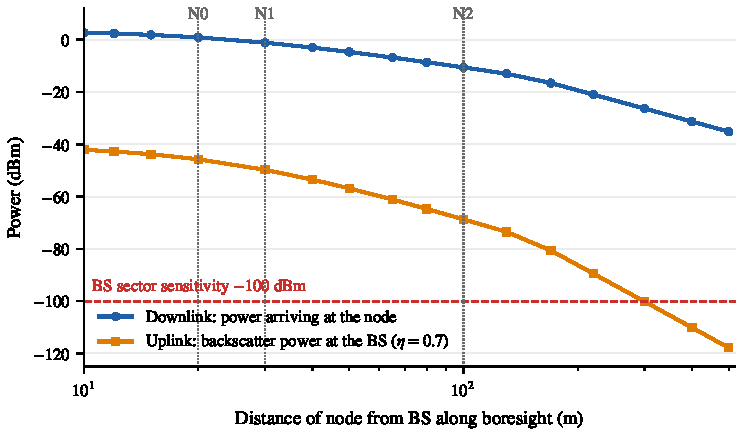
\includegraphics[width=0.88\linewidth]{fig_budget}
\caption{Downlink power at the node and uplink backscatter power at the base station against distance, for the demo's north-facing sector ($\SI{46}{dBm}$, $\SI{15}{dBi}$, $\eta=0.7$), computed by Amber. The uplink starts $\sim\SI{45}{dB}$ lower and falls twice as fast. With the demo's $\SI{-100}{dBm}$ sector sensitivity the link would close out to about $\SI{300}{m}$; the node would be energy-limited long before.}
\label{fig:budget}
\end{figure}

\paragraph{Which hop limits the system?}
A tag works only if \emph{both} conditions hold:
\begin{align*}
 &\text{(forward / energy)} && P_{\mathrm{tag}}\ \text{large enough to power the device,}\\
 &\text{(reverse / information)} && P_r\ge S_{\mathrm{rx}}.
\end{align*}
Which one fails first depends on design. For a passive tag with no storage, the
forward link usually limits: the rectifier needs of order $\SI{-20}{dBm}$ or more to
turn on. For a device with a battery or large storage the reverse
link limits. In Amber's demos the downlink is generous (milliwatts at $\le\SI{30}{m}$),
and the uplink margin at $\SI{100}{m}$ is over $30$~dB, so the energy
\emph{accumulation time} (Chapter~\ref{ch:capacitor}) rather than the link margin
decides how often a node can talk.

\begin{example}[The paper's scenario: can an RF-only node even start?]
The paper's experiment uses $\SI{30}{dBm}$ sectors with $\SI{17}{dBi}$, $\SI{1}{dBi}$ nodes and 924~MHz.
At $\SI{20}{m}$ the UMa LOS loss is $\SI{60.1}{dB}$, so the node receives
$30+17+1-60.1=\SI{-12.1}{dBm}=\SI{62}{\micro W}$; at $\SI{100}{m}$ only $\SI{-23.6}{dBm}=\SI{4.4}{\micro W}$.
Under Amber's harvesting model with the demo's $\Rs=\SI{5}{k\ohm}$ these correspond to
equivalent source voltages $\sqrt{P\Rs}\approx\SI{0.56}{V}$ and $\SI{0.15}{V}$
(Chapter~\ref{ch:harvest}), far below the $\Vhigh=\SI{1.7}{V}$ used in the demos.
Even the best case beyond $\SI{10}{m}$ gives only $\approx\SI{0.65}{V}$. \emph{Such
nodes can never wake up on RF alone}---which is why the paper operates them in
\textbf{hybrid power mode} with an external (solar) source. The thresholds and
$\Rs$ of the paper's run are not stated in the abstract; we use the demo values.
\end{example}

\section{Splitting power between harvesting and reflecting}
\label{sec:split}

An antenna captures a fixed amount of power. What it \emph{reflects} it
cannot also \emph{rectify}; to first order,
\[
 P_{\mathrm{harvest}} + P_{\mathrm{reflect}} = P_{\mathrm{captured}}.
\]
The paper describes nodes by ``a power split ratio determining how received RF
power is divided between energy harvesting and backscatter reflection.'' In Amber
that ratio is $\eta=$ \codew{Node.efficiency} $\in[0,1]$ (default~1), and the
bookkeeping is a \emph{state-dependent} one:
\begin{align}
 P_{\mathrm{backscatter}} &= \eta\,P_{\mathrm{dl}} && \text{(always computed)},\\
 P_{\mathrm{harvest}} &=
 \begin{cases}
  P_{\mathrm{dl}} & \text{node not transmitting},\\
  (1-\eta)\,P_{\mathrm{dl}} & \text{node in the \emph{transmitting} state.}
 \end{cases}
\end{align}
While the node is idle its antenna absorbs everything; while it
transmits a fraction $\eta$ is reflected and so lost to the harvester. Because
transmissions are brief this costs little energy, but the model captures the
principle that \emph{communicating and harvesting compete for the same photons}.
For Node~0 ($P_{\mathrm{dl}}=\SI{1.24}{mW}$, $\eta=0.7$) the equivalent
source voltage drops from $\SI{2.49}{V}$ to $\SI{1.36}{V}$ for the duration of a transmission.

\begin{reality}[What $\eta$ must absorb]
In Amber $\eta$ is a \emph{single scalar} that must stand for everything that
reduces the reflected \emph{information-bearing} power: the incomplete modulation depth,
the conversion of carrier power into the wanted sideband (next section),
the antenna's mismatch and structural scattering. A square-wave-shifted OOK
tag, for instance, puts only $(1/\pi)^2\approx0.10$ of the incident power into
each first sideband. The default $\eta=1$ is therefore the most optimistic choice;
the shipped demos use $0.7$. Choose it deliberately.
\end{reality}

\section{Self-interference and frequency-shifted backscatter}
\label{sec:selfint}

Recall the dynamic-range problem of Section~\ref{sec:dynrange}: the reader's own
carrier, even after $\sim\SI{25}{dB}$ of antenna isolation, is tens of dB stronger
than the reflected data. A receiver cannot filter it out if the wanted signal sits
at the \emph{same} frequency. The solution is to move the reply away
in frequency.

Let the incident carrier be $x(t)=A\cos(2\pi f_ct)$ and let the tag toggle its
reflection coefficient between $\Gamma_0$ and $\Gamma_1$ with a unit square wave
$s(t)\in\{0,1\}$ of frequency $f_s$, so that $\Gamma(t)=\Gamma_0+\Delta\Gamma\,s(t)$,
$\Delta\Gamma=\Gamma_1-\Gamma_0$. The Fourier series of the square wave is
$s(t)=\tfrac12+\tfrac{2}{\pi}\sum_{k\ \mathrm{odd}}\tfrac1k\sin(2\pi kf_st)$. The
reflected signal $y(t)=\Gamma(t)x(t)$ is therefore
\begin{align}
 y(t)&=\Big(\Gamma_0+\tfrac{\Delta\Gamma}{2}\Big)A\cos(2\pi f_ct)\label{eq:y0}\\
 &\quad+\frac{\Delta\Gamma}{\pi}A\Big[\sin\big(2\pi(f_c+f_s)t\big)-\sin\big(2\pi(f_c-f_s)t\big)\Big]+\text{odd harmonics}.\label{eq:y1}
\end{align}
Term~\eqref{eq:y0} is a copy of the carrier at $f_c$ (the
\emph{static} reflection, carrying no data). The information-bearing
energy appears at $f_c\pm f_s$ in \eqref{eq:y1}. Each first-order sideband has power
$(\Delta\Gamma/\pi)^2$ times the incident carrier power: for
$\Delta\Gamma=1$ (on--off) that is $-9.9$~dB; for a phase flip between $+1$ and
$-1$ ($\Delta\Gamma=2$) it is $-3.9$~dB. The reader now tunes its receiver to
$f_c+f_s$, where the carrier leakage is absent.

\begin{figure}[t]
\centering
\begin{tikzpicture}[x=1cm,y=1cm]
 \draw[->] (-1.0,0) -- (12.2,0) node[right,lab] {frequency};
 % carrier
 \draw[->,line width=2pt,ablue] (1.5,0) -- (1.5,3.0);
 \node[lab,ablue,align=center,anchor=south] at (1.5,3.05) {unmodulated carrier\\(dedicated subcarrier)};
 % downlink data subcarrier
 \draw[->,line width=2pt,agrey] (0.0,0) -- (0.0,1.5);
 \node[lab,agrey,align=center,anchor=south] at (-0.1,1.55) {data subcarrier\\(downlink commands)};
 % backscatter groups
 \foreach \x/\c/\n in {4.2/agreen/1,6.6/aorange/2,9.0/apurple/3}{
   \draw[->,line width=1.6pt,\c] (\x,0) -- (\x,0.55);
   \draw[->,line width=1.6pt,\c] (\x+0.3,0) -- (\x+0.3,0.4);
   \draw[->,line width=1.6pt,\c] (\x-0.3,0) -- (\x-0.3,0.4);
   \node[lab,\c,anchor=north] at (\x,-0.15) {shift $\n$};
 }
 \draw[<->,agrey] (1.5,-0.85) -- node[lab,below]{$f_{s,1}$} (4.2,-0.85);
 \draw[<->,agrey] (1.5,-1.35) -- node[lab,below]{$f_{s,2}$} (6.6,-1.35);
 \draw[<->,agrey] (1.5,-1.85) -- node[lab,below]{$f_{s,3}$} (9.0,-1.85);
 \node[lab,align=left,anchor=west] at (9.8,1.3) {\textcolor{agreen}{nodes in the same}\\\textcolor{agreen}{group share a shift:}\\\textcolor{agreen}{they can collide}\\and need SIC};
\end{tikzpicture}
\caption{Frequency-domain picture of the dual-tone downlink and frequency-shifted backscatter. A clean carrier on a dedicated subcarrier powers and illuminates the nodes; one data-bearing subcarrier carries the downlink. Each node reflects its reply at an offset $f_{s,k}$ from the carrier (shown on one side only; real sidebands appear on both). Different offsets are \emph{orthogonal}; nodes with the same offset overlap in frequency and time and must be separated by capture or SIC (Chapter~\ref{ch:sic}).}
\label{fig:spectrum}
\end{figure}

\paragraph{Frequency shifting as multiple access.}
If different nodes choose \emph{different} $f_s$, their replies land in different
frequency slots and do not collide even if they transmit simultaneously. The
paper's three \emph{subcarrier shifts} exploit exactly this: ``Distinct subcarrier
offsets provide frequency-domain separation, and successive interference
cancellation (SIC) resolves collisions among nodes sharing the same offset.''
Subcarrier shifting thus has \emph{two} roles: keeping replies away from carrier
interference, and acting as a coarse FDMA-style resource.

\begin{reality}[How Amber models subcarrier shifts]
Amber does not synthesise any spectrum. \codew{Node.subcarrier_shift} is an
\emph{integer label}; the base station groups packets by that label and
assumes that different labels are \emph{perfectly orthogonal}
(Chapter~\ref{ch:sic}). Neither carrier leakage, adjacent-shift leakage, nor the
sideband loss of Eq.~\eqref{eq:y1} is modelled explicitly---the latter is yours to place
inside $\eta$.
\end{reality}

\section{Receiving with no receiver: the passive downlink}
\label{sec:passivedl}

So far we have covered uplink. How does a $\mu$W device \emph{hear} commands?
A conventional receiver needs a low-noise amplifier, a local oscillator and a
mixer, and consumes milliwatts. A passive device instead uses an
\emph{envelope detector}: a diode followed by a low-pass filter that outputs
the slowly varying \emph{amplitude} of the incoming signal, much like a crystal
radio. It works naturally with \emph{on--off keying} (OOK): a ``1'' is
carrier present, a ``0'' is carrier absent. The 3GPP Release-19 summaries
describe exactly this: an RF envelope-detection receiver and OOK on the
reader-to-device link. The costs are poor sensitivity (typically in the region of
$\SI{-40}{dBm}$ to $\SI{-50}{dBm}$ for simple passive detectors, tens of dB
worse than an active receiver) and low data rates---which is why Amber's default
\emph{node} sensitivity is $\SI{-45}{dBm}$ while its \emph{sector} sensitivity
is $\SI{-100}{dBm}$.

\paragraph{OFDMA downlinks for passive nodes.}
Cellular networks use OFDM, whose many subcarriers are normally separated by
an FFT, which is expensive. The paper cites Zhu et al.\
\citep{zhu2022ofdma}, who demonstrate OFDMA downlink demodulation at around
$\SI{100}{\micro W}$ by replacing the digital FFT with \emph{analogue
filtering}. This is the enabling idea behind the Amber paper's \emph{dual-tone
principle}.

\paragraph{The dual-tone PRDCH.}
The paper says that Amber's physical layer is by default based on the
\emph{Physical Reader to Device Channel} (PRDCH): ``an external unmodulated
carrier occupies a dedicated OFDM subcarrier, enabling both energy harvesting
and backscatter reflection \citep{zhu2022ofdma}, while a single data-bearing
subcarrier carries downlink information from base station to node.'' Two tones,
two jobs:
\begin{enumerate}
 \item the \emph{carrier tone} is a clean sinusoid, ideal both for harvesting
   (constant, rectifier-friendly power) and as the illumination to be reflected
   (nothing to cancel except the carrier itself);
 \item the \emph{data subcarrier} carries OOK-like commands that an analogue
   filter can separate from the carrier.
\end{enumerate}
Figure~\ref{fig:spectrum} sketches this arrangement. In 3GPP's terms the
PRDCH is the physical reader-to-device channel studied in TR~38.769.

\begin{reality}[The downlink is not waveform-simulated]
In Amber a command is a Python call. It is delivered if the best downlink
power reaching the node exceeds the node's sensitivity; there are no bit errors,
no demodulation, no data-rate limit and no per-command energy cost to the
node. The \emph{carrier} is implicit and always on: the base-station behaviour
class states that nodes ``harvest energy all the time'' and that ``the schedule
only handles communication''.
\end{reality}

\section{Topologies and duplexing}

Literature distinguishes three backscatter arrangements \citep{huynh2018ambient}.
\begin{description}[leftmargin=0.5cm,font=\sffamily\bfseries]
 \item[Monostatic.] The reader transmits the carrier and receives the reflection
   (one device, or two collocated). The forward and return distances are equal,
   $P_r\propto d^{-4}$. This is Amber's arrangement.
 \item[Bistatic.] A separate \emph{carrier emitter} illuminates the tag while the
   receiver is elsewhere; $d_1\ne d_2$. This resembles 3GPP's topology~T3 (with an assisting node).
 \item[Ambient.] The carrier is an unrelated, already-present signal (TV,
   Wi-Fi, cellular \citep{liu2013ambient}); the tag has no control over it.
\end{description}
The paper describes the reference experiment as a polling protocol ``operating
in full-duplex mode''. Because the carrier is transmitted \emph{continuously} on
its own subcarrier, the base station can receive backscatter while the carrier
is on. Amber's \emph{schedule} nevertheless alternates TX (command) and RX
(reply) windows: the command is on the data subcarrier and the base station
does not listen while it sends one (Chapter~\ref{ch:bsengine}).

\begin{codemap}
\small
\begin{tabularx}{\linewidth}{@{}>{\ttfamily}p{5.6cm}X@{}}
\toprule
\normalfont\bfseries Concept & \normalfont\bfseries Code (\file{amber/})\\
\midrule
Backscatter / harvest split $\eta$ & \codew{CoverageMap.calculate_node_power}; \codew{Node.efficiency}\\
Dyadic uplink budget, Eq.~\eqref{eq:dyadicdb} & \codew{CoverageMap.compute_point_to_bs}\\
Subcarrier label & \codew{Node.subcarrier_shift}; \codew{BSBehavior._process_rx_buffer}\\
Command reception gate & \codew{BackscatterModule.receive_command}\\
Always-on carrier & documented in \code{BSBehavior}; no explicit object\\
\bottomrule
\end{tabularx}
\end{codemap}

\section{Chapter summary}
\begin{itemize}
 \item Backscatter saves energy by switching a reflection instead of generating a carrier; the switch alternates between absorbing ($\Gamma\approx0$) and reflecting ($|\Gamma|\approx1$).
 \item The dyadic link $P_r=P_tG_tG_rG_a^2\,\eta\,L(d_1)L(d_2)$ has a doubled path-loss exponent; Amber implements it as two chained hops.
 \item $\eta$ splits received power between reflection and harvesting; a transmitting node harvests only $(1-\eta)P_{\mathrm{dl}}$.
 \item A square-wave switch creates sidebands at $f_c\pm f_s$ carrying $(\Delta\Gamma/\pi)^2$ of the power; shifting the reply away from the carrier defeats self-interference and enables frequency-domain multiple access.
 \item Passive devices receive with envelope detectors; the PRDCH dual-tone design pairs a clean carrier with one data subcarrier.
\end{itemize}

\section*{Exercises}
\begin{exercise}
Derive Eq.~\eqref{eq:dyadic} step by step. If both $d_1$ and $d_2$ double, by how many dB does $P_r$ change in free space? By how many dB does the \emph{downlink} power change?
\end{exercise}
\begin{exercise}
A reader transmits $\SI{36}{dBm}$ through a $\SI{9}{dBi}$ antenna at $\SI{915}{MHz}$. A tag with a $\SI{2}{dBi}$ antenna and $\eta=0.3$ is $\SI{4}{m}$ away; the same antenna receives. Compute the free-space power the tag captures and the power returned to the reader. (Take the reader receive gain equal to its transmit gain.)
\end{exercise}
\begin{exercise}
Using Eq.~\eqref{eq:y1}, find the fraction of incident power in one first-order sideband when the tag toggles between $\Gamma_0=0$ and $\Gamma_1=-0.8$. What $\eta$ would you configure in Amber to include this loss?
\end{exercise}
\begin{exercise}
In Amber, Node~1 (at $\SI{30}{m}$) transmits and its \code{efficiency} is $0.7$. By how many dB does the harvested power fall while it transmits? Repeat for $\eta=0.2$ and $\eta=1.0$.
\end{exercise}
\begin{exercise}
Explain, with reference to Figure~\ref{fig:spectrum}, why nodes assigned the \emph{same} subcarrier shift can collide but nodes with \emph{different} shifts cannot, and what resource this resembles in a cellular system.
\end{exercise}

\chapter{Energy Sources and RF Harvesting}
\label{ch:harvest}

\begin{defbox}[In this chapter you will learn]
\begin{itemize}
 \item which ambient energy sources can power a node, and roughly how much each delivers;
 \item how a rectenna turns RF into DC and why its efficiency depends strongly on input power;
 \item Amber's harvesting model: how received power becomes an \emph{equivalent source voltage} behind a series resistor, and what that implies about how much energy reaches the capacitor;
 \item the three \emph{power modes}---wireless power transfer, external, hybrid---and the difference between combining them by \emph{max} and by \emph{sum};
 \item how an external energy trace is replayed, and a surprise about the shipped trace.
\end{itemize}
\end{defbox}

\section{Where can the energy come from?}
\label{sec:sources}

``Ambient'' in Ambient IoT refers to the environment as the supplier of energy
and, sometimes, of the carrier. The main candidates differ by orders of magnitude.

\begin{center}
\small
\renewcommand{\arraystretch}{1.15}
\begin{tabularx}{\linewidth}{@{}>{\sffamily\bfseries}p{3.4cm}>{\raggedright}p{3.8cm}X@{}}
\toprule
Source & Typical power density & Remarks\\
\midrule
Outdoor sunlight & $\sim\SI{10}{mW/cm^2}$ and more & Very high, intermittent (day/night, shade)\\
Indoor light & $\sim\SI{10}{}$--$\SI{100}{\micro W/cm^2}$ & Moderate; depends on lighting\\
Thermal gradients & tens of $\si{\micro W/cm^2}$ & Needs a temperature difference\\
Vibration & $\sim\SI{100}{\micro W/cm^3}$ & Machinery, vehicles\\
Ambient RF & $\ll\SI{1}{\micro W/cm^2}$ & Very low except near a transmitter\\
\emph{Dedicated} RF (carrier) & depends on distance & Controlled; what Amber's base stations provide\\
\bottomrule
\end{tabularx}
\end{center}
\noindent\emph{Order-of-magnitude values commonly quoted in the energy-harvesting literature; actual numbers vary widely with conditions.}

Ambient RF alone is too weak to be dependable, so 3GPP Ambient IoT relies on
the network itself to \emph{beam} energy at the devices: the base station's carrier
is both the power source and the illumination for backscatter. A node can
additionally use a second source---typically light---so that it can wake up even
where the RF field is weak. Amber lets you model exactly that combination.

\section{The RF harvesting chain}
\label{sec:rectenna}

A \emph{rectenna} (rectifying antenna) consists of
\begin{enumerate}
 \item the antenna, which captures the RF power $P_{\mathrm{dl}}$;
 \item an impedance-matching network;
 \item a rectifier---diodes or transistors configured as a voltage multiplier---that converts the oscillating RF voltage into DC;
 \item a smoothing capacitor and a power-management stage that feed the storage element.
\end{enumerate}
The \emph{RF-to-DC conversion efficiency} $\eta_{\mathrm{rf\text{-}dc}}=P_{\mathrm{dc}}/P_{\mathrm{rf}}$
depends strongly on the input power, because a diode barely conducts until the
RF voltage exceeds its threshold. At very low input power (below roughly
$\SI{-20}{dBm}$ for commonly used devices) the efficiency collapses, and many
rectifiers cannot output anything usable at all---the \emph{cold-start}
problem. At moderate power the efficiency peaks (tens of percent) and at high
power the diode breaks down. A rectenna therefore has a \emph{minimum input power}
below which the harvested energy is effectively zero, however long you wait.
This is why, in a real deployment, the \emph{forward link} often limits range.

\begin{reality}[Amber has no rectifier curve]
In Amber every watt of received RF power reaches the harvester: effectively
$\eta_{\mathrm{rf\text{-}dc}}=1$ at all input levels, with no turn-on threshold,
no saturation and no cold start. The code comment simply converts received
power to DC power. If you need a realistic harvester, the hook is the single
conversion in \codew{CoverageMap.calculate_node_power} (Exercise~\ref{ex:rectifier}).
\end{reality}

\section{Amber's harvesting model}
\label{sec:amberharvest}

\subsection{From power to an equivalent source}

The capacitor model of Chapter~\ref{ch:capacitor} is driven by a
\emph{voltage} source in series with a resistor $\Rs$. The controller therefore
turns the harvested power $P_h$ (a number in dBm stored in \codew{node.harvesting_power_dbm})
into an equivalent open-circuit voltage by
\begin{equation}
 \Vs=\sqrt{P_h\,\Rs},\qquad\text{i.e. } P_h=\frac{\Vs^{2}}{\Rs}.
\label{eq:vsrc}
\end{equation}
This is the usual $P=V^2/R$ read backwards. Physically it says: ``a source of
internal resistance $\Rs$ and open-circuit voltage $\Vs$ would \emph{dissipate} $P_h$
if short-circuited into a resistance equal to its own''. It is a modelling device, not a
circuit that exists on a board; but its consequences are physical and worth
understanding.

\begin{intuition}[How much of $P_h$ actually reaches the capacitor?]
When the capacitor sits at voltage $V$, the current is $(\Vs-V)/\Rs$ and the power
\emph{delivered into the capacitor} is $V(\Vs-V)/\Rs$. With $x=V/\Vs$,
\[
 P_{\mathrm{into\ C}}(x)=P_h\,x(1-x),
\]
which is a parabola with maximum $P_h/4$ at $x=\tfrac12$ (the familiar
\emph{maximum-power-transfer} theorem). So the \emph{effective} harvesting efficiency of
the model is at most $25\%$ and falls to zero as the capacitor approaches $\Vs$.
For Node~0 at $V=\SI{1.5}{V}$, $x=0.60$ and the capacitor receives
$0.24\,P_h\approx\SI{0.30}{mW}$ of the $\SI{1.24}{mW}$ nominally harvested; the
rest is dissipated in $\Rs$. The charge-only update of the simulator reproduces this behaviour exactly
(Chapter~\ref{ch:capacitor}).
\end{intuition}

\subsection{Three power modes}

The harvest power of each node is recomputed from the pre-computed downlink power
by \codew{CoverageMap.calculate_node_power}, according to \codew{node_energy_mode}.
Let $P_{\mathrm{dl}}$ be the best downlink power (in watts) at the node, $\eta$ its
\code{efficiency}, $P_{\mathrm{ext}}$ the instantaneous power of the external source,
and $\mathbb{1}_{\mathrm{tx}}$ be $1$ while the node is in its \emph{transmitting} state and $0$ otherwise.

\begin{center}
\small
\renewcommand{\arraystretch}{1.25}
\begin{tabularx}{\linewidth}{@{}>{\ttfamily}l>{\raggedright}X>{\raggedright\arraybackslash}X@{}}
\toprule
\normalfont\bfseries Mode & \normalfont\bfseries Harvested power $P_h$ & \normalfont\bfseries Backscatter power\\
\midrule
"wpt" & $P_{\mathrm{dl}}\,\big(1-\eta\,\mathbb{1}_{\mathrm{tx}}\big)$ & $\eta P_{\mathrm{dl}}$\\
"external" & $P_{\mathrm{ext}}$ (RF is \emph{not} harvested) & $\eta P_{\mathrm{dl}}$\\
"hybrid" & $\max\big(P_{\mathrm{wpt}},P_{\mathrm{ext}}\big)$ if \codew{combine_mode="max"} (default), else $P_{\mathrm{wpt}}+P_{\mathrm{ext}}$ & $\eta P_{\mathrm{dl}}$\\
\bottomrule
\end{tabularx}
\end{center}
where $P_{\mathrm{wpt}}=P_{\mathrm{dl}}(1-\eta\,\mathbb{1}_{\mathrm{tx}})$. Three points deserve emphasis.
\begin{enumerate}
 \item The backscatter power is $\eta P_{\mathrm{dl}}$ in \emph{every} mode: a node powered by solar light still
   needs the base station's carrier to reflect.
 \item ``Hybrid'' does \emph{not} mean ``sum''. With the default \codew{combine_mode="max"}
   the node simply uses whichever source is stronger at that instant.
 \item The base station carriers are not summed either: the node harvests the
   \emph{best} sector's power only (\code{best_pw_w}), a conservative simplification when several
   carriers overlap.
\end{enumerate}

\begin{example}[Why the hybrid node of the demos lives on sunlight]
In the broadcast demos Node~2, $\SI{100}{m}$ from the base station, receives
$P_{\mathrm{dl}}=\SI{-10.57}{dBm}=\SI{87.7}{\micro W}$, giving $\Vs=\sqrt{87.7\times10^{-6}\cdot5000}=\SI{0.662}{V}$ from RF. The steady-state voltage
(Chapter~\ref{ch:capacitor}) is $\Vs\Rl/(\Rl+\Rs)=\SI{0.63}{V}\ll\Vhigh$, so from RF alone Node~2 would
\emph{never} start. The solar trace has mean power $\SI{1.43}{mW}$ ($\Vs\approx\SI{2.66}{V}$),
$16\times$ larger. Because \codew{combine_mode="max"} picks the larger term, \emph{the RF contribution is
irrelevant}; Node~2's harvesting is solar-only, which is why it activates fastest
and sends the most packets (Figure~\ref{fig:sawtooth}). With \codew{combine_mode="sum"} the two would add in power:
$\sqrt{(87.7+1433)\,\si{\micro W}\cdot5000}=\SI{2.76}{V}$.
\end{example}

\section{The external source}
\label{sec:envsource}

\codew{EnvEnergySource} is a SimPy actor that \emph{replays a recorded trace}.
It reads an Excel file, takes one column (default \code{V_IM}) of voltages, and at
every simulation millisecond sets
\[
 P_{\mathrm{ext}}(t_k)=\frac{V_k^{2}}{R},\qquad R=\code{resistance}\ (\SI{1}{\ohm}\ \text{default; the demos pass }R_s=\SI{5}{k\ohm}).
\]
After the last row it loops. The object exposes the current value as
\code{ext_power}; the coverage map reads it through the callback
\codew{node_ext_power_fn}, which in the demos is
\codew{lambda node: energy_source.ext_power}. Because the callback ignores its
argument, \emph{all nodes see the same external power at the same instant}: there is no
spatial variation (shading) of the solar source.

When \code{resistance} equals the controller's $\Rs$, the round trip
$V\to P=V^2/R\to\sqrt{P\Rs}$ returns the recorded voltage unchanged. In the demos the trace's \code{V_IM}
column is thus directly the equivalent source voltage of the solar harvester.

\begin{reality}[The ``300-second'' trace is three seconds long]
The file \file{threehundred_seconds_stable.xlsx} contains $2999$ rows with a time
step of $\SI{1}{ms}$ (the last time stamp is $\SI{2.998}{s}$). Since
\codew{EnvEnergySource} consumes one row per millisecond and loops, the
trace is \emph{three seconds long}, repeated. Its statistics are: $V_{IM}$ between
$1.78$ and $\SI{3.01}{V}$, mean $\SI{2.66}{V}$, standard deviation $\SI{0.25}{V}$, i.e.\ a
nearly constant $\approx\SI{1.4}{mW}$ source ($\SI{1.56}{dBm}$). For simulations of tens of
seconds the periodicity of the trace could show up as spurious structure.
\end{reality}

\section{When is harvesting updated?}

Harvest power is recomputed \emph{every millisecond for every node} inside the
controller loop (Chapter~\ref{ch:controller}). For a pure WPT node this matters
only when its state toggles into or out of \emph{transmitting} (the $1-\eta$
factor); for a node with an external source it also tracks the trace. The comment
in the controller source explains the economy: if no coverage map or downlink
results are supplied, ``wpt is static, no need to recalculate every ms''.

\begin{codemap}
\small
\begin{tabularx}{\linewidth}{@{}>{\ttfamily}p{5.0cm}X@{}}
\toprule
\normalfont\bfseries Concept & \normalfont\bfseries Code\\
\midrule
Harvest/backscatter bookkeeping & \codew{CoverageMap.calculate_node_power} (\file{propagation.py})\\
Hybrid combination & \codew{combine_mode} (\code{"max"} default)\\
Power to source voltage, Eq.~\eqref{eq:vsrc} & \codew{Controller.run}: \codew{(power_w * R_series) ** 0.5}\\
Solar trace & \codew{EnvEnergySource} (\file{energy.py})\\
Callback & \codew{CoverageMap.node_ext_power_fn}\\
\bottomrule
\end{tabularx}
\end{codemap}

\section{Chapter summary}
\begin{itemize}
 \item Sunlight dwarfs ambient RF by orders of magnitude; 3GPP therefore beams a dedicated carrier at the devices.
 \item Real rectennas have a minimum input power and a power-dependent efficiency; Amber omits both.
 \item Amber converts harvested power to a Th\'evenin-style source $\Vs=\sqrt{P_h\Rs}$; at most $P_h/4$ ever reaches the capacitor.
 \item Modes: wpt, external, hybrid (max or sum). Backscatter always uses the base-station carrier.
 \item The shipped trace is $3$~s long, shared by all nodes, and effectively a $\SI{2.7}{V}$ source.
\end{itemize}

\section*{Exercises}
\begin{exercise}
The solar trace has mean voltage $\SI{2.66}{V}$ and $R=\SI{5}{k\ohm}$. Compute the external power in mW and dBm. (Careful: use the mean of $V^2$ or of $V$? How big is the difference given $\sigma=\SI{0.25}{V}$?)
\end{exercise}
\begin{exercise}
In hybrid mode, $P_{\mathrm{wpt}}=\SI{1}{mW}$ and $P_{\mathrm{ext}}=\SI{1.4}{mW}$. Compute the equivalent source voltage ($\Rs=\SI{5}{k\ohm}$) for \codew{combine_mode="max"} and for \code{"sum"}.
\end{exercise}
\begin{exercise}
A WPT node with $\eta=0.7$ receives $\SI{1}{mW}$. By how many dB does its harvested power drop while it is transmitting? What if $\eta=0.2$?
\end{exercise}
\begin{exercise}
For which received downlink power $P_{\mathrm{dl}}$ can a WPT-only node eventually reach $\Vhigh=\SI{1.7}{V}$ with $\Rs=\SI{5}{k\ohm}$ and $\Rl=\SI{100}{k\ohm}$? Express your answer in $\si{\micro W}$ and dBm. (Hint: you need the steady-state formula of Chapter~\ref{ch:capacitor}.)
\end{exercise}
\begin{exercise}\label{ex:rectifier}
Suppose you want to include an RF-to-DC efficiency $\eta_{\mathrm{rf\text{-}dc}}(P_{\mathrm{in}})$ that is zero below $\SI{-20}{dBm}$ and $0.3$ above. Where in the pipeline $P_{\mathrm{dl}}\to\Vs$ would you insert it, and how would this change the paper's scenario of Section~\ref{sec:twoway}?
\end{exercise}

\chapter{Energy Storage: The Capacitor and Intermittent Operation}
\label{ch:capacitor}

\begin{defbox}[In this chapter you will learn]
\begin{itemize}
 \item the circuit model of a harvester feeding a capacitor through a series resistor, with leakage and a load;
 \item how to solve it: time constants, steady state, charge time, sustainable current;
 \item how Amber discretises the model with a 1\,ms step and why the discretisation is accurate;
 \item why a node needs \emph{two} voltage thresholds (hysteresis), how big an ``energy window'' they create, and the \emph{duty-cycle theorem} $D=P_{\mathrm{in}}/P_{\mathrm{active}}$;
 \item the \emph{energy-accounting} subtlety in the simulator's charge-while-active step, with a measured size of its effect.
\end{itemize}
\end{defbox}

\section{Why a capacitor?}

A harvesting node needs somewhere to \emph{accumulate} energy between its brief
bursts of activity. A rechargeable battery has high energy density but wears out,
leaks chemically and is costly; a \emph{capacitor} (or supercapacitor) stores less but
can be charged and discharged almost without limit, which suits devices intended to
live for a decade. Its great limitation is that its voltage is not constant:
\begin{equation}
 Q=CV,\qquad E=\tfrac12CV^{2},\qquad i=C\frac{\mathrm{d}V}{\mathrm{d}t}.
\label{eq:cap}
\end{equation}
Draining a capacitor lowers its voltage, and electronics need a minimum voltage.
The \emph{usable} energy is therefore only that between two voltages, a point
that drives the threshold logic of Section~\ref{sec:hysteresis}.

\section{The circuit}
\label{sec:circuit}

Amber's capacitor sees the circuit of Figure~\ref{fig:rccircuit}: the harvester
as a source $\Vs$ behind a series resistance $\Rs$ (Section~\ref{sec:amberharvest}), the
capacitor $C$, a parallel \emph{leakage} resistance $\Rl$ that models
self-discharge, and a load that draws a current $I_L$ chosen by the node's
state.

\begin{figure}[t]
\centering
\begin{circuitikz}[american,scale=0.95,transform shape]
 \draw (0,0) to[V,invert,l=$V_{\mathrm{src}}$] (0,2.6) to[R,l=$R_{\mathrm{s}}$] (3.0,2.6) -- (4.4,2.6);
 \draw (4.4,2.6) to[C,l=$C$,v=$V$,*-*] (4.4,0) -- (0,0);
 \draw (4.4,2.6) -- (6.8,2.6) to[R,l=$R_{\mathrm{l}}$,*-*] (6.8,0) -- (4.4,0);
 \draw (6.8,2.6) -- (9.2,2.6) to[I,l=$I_L$,*-*] (9.2,0) -- (6.8,0);
 \node[lab,align=center,anchor=north] at (0,-0.1) {harvester\\(Ch.~\ref{ch:harvest})};
 \node[lab,align=center,anchor=north] at (6.8,-0.1) {leakage};
 \node[lab,align=center,anchor=north] at (9.2,-0.1) {node load\\(Ch.~\ref{ch:controller})};
\end{circuitikz}
\caption{Equivalent circuit of Amber's energy store. Typical demo values: $\Rs=\SI{5}{k\ohm}$, $\Rl=\SI{100}{k\ohm}$, $C=\SI{300}{\micro F}$ (\SI{200}{\micro F} in the SIC demo); the load current $I_L$ takes values \SIrange{0.14}{5}{mA} depending on the node's state.}
\label{fig:rccircuit}
\end{figure}

Kirchhoff's current law at the capacitor node gives the governing equation
\begin{equation}
 C\frac{\mathrm{d}V}{\mathrm{d}t}\;=\;\frac{\Vs-V}{\Rs}\;-\;\frac{V}{\Rl}\;-\;I_L.
\label{eq:ode}
\end{equation}

\section{Solving it}
\label{sec:ode}

For a constant $\Vs$ and $I_L$, Eq.~\eqref{eq:ode} is linear first order. Define
\begin{equation}
 \tau=(\Rs\parallel\Rl)\,C=\frac{\Rs\Rl}{\Rs+\Rl}\,C,\qquad
 V_\infty=\big(\Vs-I_L\Rs\big)\frac{\Rl}{\Rl+\Rs}.
\label{eq:tauvinf}
\end{equation}
Then
\begin{equation}
 V(t)=V_\infty+\big(V_0-V_\infty\big)\,\e^{-t/\tau}.
\label{eq:vsol}
\end{equation}
Look at what the pieces mean.

\paragraph{Time constants.}
With the demo's $\Rs=\SI{5}{k\ohm}$, $\Rl=\SI{100}{k\ohm}$, $C=\SI{300}{\micro F}$:
the charging constant is $\tau_c=\Rs C=\SI{1.5}{s}$, the leakage constant
$\tau_\ell=\Rl C=\SI{30}{s}$, and the effective constant
$\tau=\SI{1.43}{s}$ is dominated by charging.

\paragraph{Steady state.}
With no load ($I_L=0$) the capacitor settles at
$\Vs\,\Rl/(\Rl+\Rs)$: a \emph{voltage divider} between the series and
leakage resistances. With $\Rl/\Rs=20$ the final voltage is $95.2\%$ of $\Vs$; leakage steals about
$5\%$. If a load draws $I_L$, the steady voltage falls by $I_L\Rs\,\Rl/(\Rl+\Rs)$.
A node is \emph{energy-starved} if $V_\infty<\Vlow$ for its typical load: it can never
sustain operation.

\paragraph{Sustainable current.}
At voltage $V$ the harvester can supply a steady current $(\Vs-V)/\Rs$ and leakage takes
$V/\Rl$, so the \emph{sustainable} load is
\begin{equation}
 I_{\max}(V)=\frac{\Vs-V}{\Rs}-\frac{V}{\Rl}.
\end{equation}
At $V=\SI{1.5}{V}$, Node~0 ($\Vs=\SI{2.49}{V}$) can sustain $\SI{182}{\micro A}$, which
exceeds the $\SI{140}{\micro A}$ listening current: it could idle in the listening state indefinitely.
Node~1 ($\Vs=\SI{1.97}{V}$) can sustain only $\SI{79}{\micro A}$, so even
continuous listening would drain it; it \emph{must} duty-cycle. This one-line
calculation predicts a lot about who will be awake.

\paragraph{Time to reach a threshold.}
Solving Eq.~\eqref{eq:vsol} for $V(t)=V_{\mathrm{th}}$ starting at $V_0<V_{\mathrm{th}}<V_\infty$:
\begin{equation}
 t_{\mathrm{th}}=\tau\,\ln\frac{V_\infty-V_0}{V_\infty-V_{\mathrm{th}}}.
\label{eq:tth}
\end{equation}

\begin{example}[Activation times of the demo nodes]
From $V_0=0$ with $\Vhigh=\SI{1.7}{V}$ and no load:
\begin{center}
\small
\renewcommand{\arraystretch}{1.1}
\begin{tabular}{@{}lrrrr@{}}
\toprule
Node & $\Vs$ (V) & $V_\infty$ (V) & $t_{1.7\,\mathrm{V}}$ (s) & Remark\\
\midrule
Node 0, WPT, \SI{20}{m} & 2.486 & $2.37$ (clamped to $2.0$) & 1.81 & \\
Node 1, WPT, \SI{30}{m} & 1.971 & 1.88 & 3.37 & slower\\
Node 2, RF only & 0.662 & 0.63 & never & $V_\infty<\Vhigh$\\
Node 2, solar (mean) & 2.665 & 2.54 (clamped to $2.0$) & 1.58 & what the demo uses\\
\bottomrule
\end{tabular}
\end{center}
The measured activations in Figure~\ref{fig:sawtooth} ($\approx1.8$, $\approx3.4$ and
$\approx\SI{1.4}{s}$) agree; Node~2's slightly earlier activation reflects the trace's initial
values ($\approx\SI{2.7}{V}$ to $\SI{3.0}{V}$). A random start-up delay of up to $\SI{2}{s}$ (Chapter~\ref{ch:controller})
can postpone activation further.
\end{example}

\begin{figure}[t]
\centering
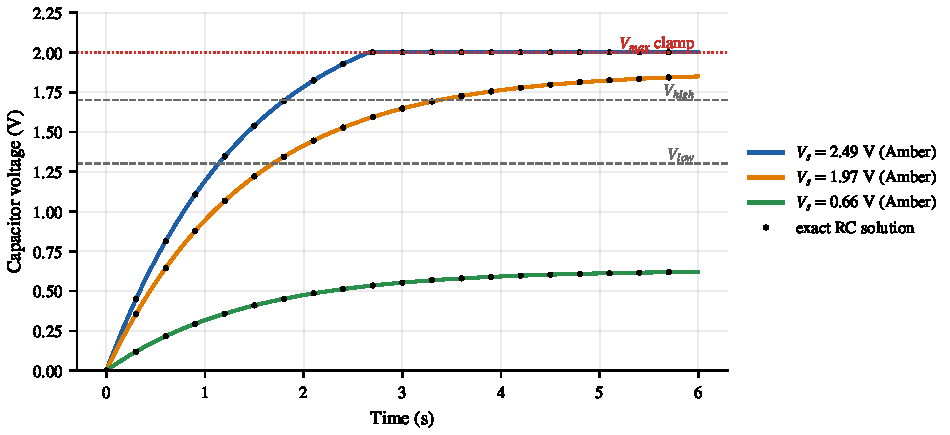
\includegraphics[width=0.9\linewidth]{fig_cap_charge}
\caption{Charging from empty for three source voltages. Lines: Amber's discrete update; dots: the exact solution Eq.~\eqref{eq:vsol} (they coincide). The top curve is clipped by $\Vmax=\SI{2}{V}$. The bottom curve ($\Vs=\SI{0.66}{V}$) saturates far below $\Vlow$ and never activates a node.}
\label{fig:capcharge}
\end{figure}

\section{Discretisation: how Amber steps the equation}
\label{sec:discretisation}

Amber advances the capacitor in steps of $\Delta t=\SI{1}{ms}$. Because
$\Delta t/\tau\approx7\times10^{-4}\ll1$, even a crude scheme is accurate;
Amber uses a hybrid of two methods per step. For the charge-only case:
\begin{equation}
 V_{k+1}=V_k\,\e^{-\Delta t/(\Rl C)}+\frac{\Delta t}{\Rs C}\big(\Vs-V_k\big).
\label{eq:chargestep}
\end{equation}
The leakage term is integrated \emph{exactly} (an exponential decay), the source
term by one \emph{explicit-Euler} step; this is an \emph{operator-splitting}
scheme with error $O(\Delta t)$ per unit time. Explicit Euler is stable here because $\Delta t/(\Rs C)\ll2$.

\begin{keyidea}[Verified: the charge-only step is accurate to $2\times10^{-4}$ V]
Starting from $\SI{1.0}{V}$ with $\Vs=\SI{2.5}{V}$ (unclamped), after $\SI{1}{s}$ Amber gives
$\SI{1.69536}{V}$; the exact solution Eq.~\eqref{eq:vsol} gives $\SI{1.69519}{V}$.
\end{keyidea}

\subsection{The four step types}

The \code{Capacitor} class implements four updates; the controller selects among them by sending a SimPy \emph{interrupt}
with a string cause (Chapter~\ref{ch:architecture}). Each ends with a clamp to $[0,\Vmax]$ ($\Vmax=\SI{2}{V}$, ``physical clamp / PMIC max'').
\begin{center}
\small
\renewcommand{\arraystretch}{1.3}
\begin{tabularx}{\linewidth}{@{}>{\ttfamily}p{3.8cm}X@{}}
\toprule
\normalfont\bfseries Cause (interrupt) & \normalfont\bfseries Update (per $\Delta t$)\\
\midrule
\codew{capacitor_charging} & Eq.~\eqref{eq:chargestep}: charge from $\Vs$ with leakage. Used while off or waiting for a slot.\\
\codew{capacitor_full} & Leakage only: $V\leftarrow V\,\e^{-\Delta t/(\Rl C)}$. Sent once, at activation.\\
\codew{capacitor_discharge} & Load only: $\Delta E=V I\Delta t$, $V\leftarrow\sqrt{V^2-2\Delta E/C}-V(1-\e^{-\Delta t/\Rl C})$. \emph{Not sent by the shipped controller.}\\
\codew{capacitor_charge_and_discharge} & Simultaneous: $I_c=\max\{(\Vs-V)/\Rs,0\}$; $E\leftarrow\max\{E+\Vs I_c\Delta t-VI_L\Delta t,\,0\}$; $V\leftarrow\sqrt{2E/C}\,\e^{-\Delta t/\Rl C}$. Used in every active state.\\
\bottomrule
\end{tabularx}
\end{center}

\paragraph{The capacitor is passive.}
The \code{Capacitor}'s own process merely \emph{waits}; its voltage changes
\emph{only when the controller interrupts it}. Because the controller issues exactly one interrupt per millisecond, one controller tick equals
one capacitor step. As we verified experimentally, SimPy schedules an interrupt with
\emph{urgent} priority, so the capacitor reacts within the \emph{same} millisecond, before ordinary events at that time. A capacitor created without a
controller would hold its voltage forever, with no leakage.

\subsection{Discharge}
Under a constant-current load $I_L$ the leakage-free solution of Eq.~\eqref{eq:ode} is
$V(t)=V_0-I_Lt/C$. Amber states this via \emph{energy}: the load draws power $VI_L$,
so in one step $\Delta E=VI_L\Delta t$ and $V'=\sqrt{V^2-2\Delta E/C}\approx V-I_L\Delta t/C$ for small steps---the same result. A $\SI{15}{ms}$, $\SI{5}{mA}$ transmission therefore
lowers a capacitor of $\SI{300}{\micro F}$ by
\[
 \Delta V=\frac{I_L\,T}{C}=\frac{5\times10^{-3}\cdot15\times10^{-3}}{300\times10^{-6}}=\SI{0.25}{V},
\]
which is exactly the step height of the sawtooth in Figure~\ref{fig:sawtooth} (we measured $1.5\to1.248$~V
for the load-only step, against $1.25$~V for ideal constant current).

\section{Thresholds, hysteresis and the energy window}
\label{sec:hysteresis}

A node cannot operate at an arbitrarily low voltage, and turning it on at the
\emph{same} voltage at which it turns off would cause \emph{chattering}: starting up draws current,
the voltage sags below the threshold, the node switches off, the voltage recovers, and so on. The remedy
is \emph{hysteresis}, familiar from the Schmitt trigger and from the under-voltage lock-out of
energy-harvesting power-management ICs: two thresholds.
\begin{itemize}
 \item \textbf{$\Vhigh$} (demo: $\SI{1.7}{V}$): the node switches \emph{on} when $V\ge\Vhigh$.
 \item \textbf{$\Vlow$} (demo: $\SI{1.3}{V}$): the node switches \emph{off} when $V\le\Vlow$.
\end{itemize}
\begin{figure}[t]
\centering
\begin{tikzpicture}[node distance=5.2cm]
 \node[st,draw=agrey,fill=lightgrey,minimum width=3.4cm] (off) {Charging (off)\\harvest only, no load};
 \node[st,draw=agreen,fill=lightgreen,minimum width=3.4cm,right=of off] (on) {Active\\duty cycle (load on)};
 \draw[->,thick] (off.north) to[bend left=35] node[lab,above,align=center]{$V\ge\Vhigh$\\and start-up delay over} (on.north);
 \draw[->,thick] (on.south) to[bend left=35] node[lab,below]{$V\le\Vlow$} (off.south);
\end{tikzpicture}
\caption{Hysteretic two-state behaviour of an energy-harvesting node. The $\SI{0.4}{V}$ gap between thresholds sets the size of the usable energy window.}
\label{fig:hyst}
\end{figure}
The energy available between the thresholds is
\begin{equation}
 \Delta E=\tfrac12C\big(\Vhigh^2-\Vlow^2\big)=\tfrac12(300\,\mu\mathrm{F})(1.7^2-1.3^2)=\SI{180}{\micro J}.
\end{equation}
The stored energy at $\SI{1.7}{V}$ is $\SI{433.5}{\micro J}$, of which only $41\%$ is usable;
the rest remains as the unusable floor $\tfrac12C\Vlow^2=\SI{253.5}{\micro J}$. A
larger $C$ gives a larger window (longer bursts, longer recharge); a wider gap does too.

\paragraph{How many packets fit in one window?}
We will see in Chapter~\ref{ch:controller} that one full node cycle (listen, sense, process, transmit)
consumes about $\SI{125}{\micro J}$, of which $90\%$ is the $\SI{15}{ms}$
transmission. The window of $\SI{180}{\micro J}$ would therefore hold only $\approx1.4$ cycles without
harvesting. The measured behaviour is a useful check on this arithmetic. In a $\SI{20}{s}$ run of the broadcast demo, Node~0 completed
$23$ charge cycles and sent $47$ packets, Node~1 sent $18$ in $9$ cycles and Node~2 sent $56$ in $27$ cycles:
\textbf{about two packets per saw-tooth tooth}. The first transmission of a tooth runs to completion
($\SI{15}{ms}$); the second is typically \emph{cut short}, because $V$ reaches $\Vlow$ after only
$9$--$\SI{11}{ms}$ (visible in Figure~\ref{fig:fsmzoom}). We return to this in Chapter~\ref{ch:controller}.

\begin{keyidea}[Design rule: the window must cover an atomic burst]
If an operation cannot be interrupted (a radio transmission, a flash write), the energy window
$\tfrac12C(\Vhigh^2-\Vlow^2)$ minus what the node has already spent must exceed the energy of that atomic burst, or
the node will die in the middle of it. Amber does \emph{not} enforce this: the node simply powers
down whenever $V\le\Vlow$, wherever it happens to be in its state machine.
\end{keyidea}

\subsection{The duty-cycle theorem}

Let the net charging power into the capacitor be $P_{\mathrm{in}}$ while the node is off, and let the node draw
$P_{\mathrm{act}}>P_{\mathrm{in}}$ while active (approximating both as constant). One cycle consists of
recharging by $\Delta E$ and then spending it:
\[
 T_c=\frac{\Delta E}{P_{\mathrm{in}}},\qquad T_a=\frac{\Delta E}{P_{\mathrm{act}}-P_{\mathrm{in}}}.
\]
The fraction of time the node is active is
\begin{equation}
 D=\frac{T_a}{T_a+T_c}=\frac{\dfrac1{P_{\mathrm{act}}-P_{\mathrm{in}}}}{\dfrac1{P_{\mathrm{act}}-P_{\mathrm{in}}}+\dfrac1{P_{\mathrm{in}}}}
 =\frac{P_{\mathrm{in}}}{P_{\mathrm{act}}}.
\label{eq:duty}
\end{equation}
\begin{keyidea}[Duty-cycle theorem]
The long-run fraction of time an intermittently powered node is active equals the
ratio of harvested power to active-mode power, \emph{independent of the energy window}
$\Delta E$. The window ($C$, $\Vhigh$, $\Vlow$) determines only the \emph{granularity}: how long each active
burst and each recharge pause lasts, not how much activity there is on average.
\end{keyidea}
Energy neutrality ($\overline{P}_{\mathrm{consumed}}=\overline{P}_{\mathrm{in}}$) is Eq.~\eqref{eq:duty} in disguise.
For Node~0 at $V\approx\SI{1.5}{V}$ the capacitor receives about $\SI{0.30}{mW}$ (Section~\ref{sec:amberharvest}); if the node
transmitted continuously ($\SI{7.5}{mW}$ at $\SI{1.5}{V}$) it could be active only $D\approx4\%$ of the time.

\subsection{What the node forgets}
In the language of \emph{intermittent computing} \citep{lucia2017} a power failure erases volatile state. Amber's controller resets its
state machine to \emph{listening} at each reactivation, but \emph{keeps} the last processed sensor value
and the node's protocol state (for example, whether it is registered). That models non-volatile memory for
registration; a design that loses registration at every outage would behave differently.

\begin{reality}[The active-mode step credits source energy, not delivered energy]
The charge-only step, Eq.~\eqref{eq:chargestep}, is the exact RC behaviour: the power delivered into the capacitor is $P_h\,x(1-x)$ (Figure~\ref{fig:powertransfer}).
The \emph{charge-and-discharge} step used in every active state computes the energy gained as $\Vs\,I_c\,\Delta t$, where
$I_c=(\Vs-V)/\Rs$. That is the energy \emph{drawn from the source},
which includes the heat dissipated in $\Rs$; the energy actually stored is $V\,I_c\,\Delta t$. The simulator therefore over-credits harvesting by the factor $\Vs/V$ whenever a node is active.
\begin{figure}[H]
\centering
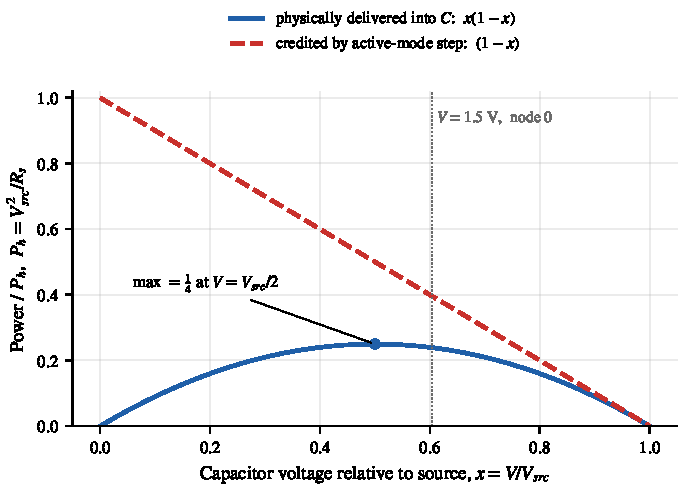
\includegraphics[width=0.55\linewidth]{fig_power_transfer}
\caption{Power delivered into $C$ (solid) versus the power credited by the active-mode step (dashed), both relative to $P_h=\Vs^2/\Rs$.}
\label{fig:powertransfer}
\end{figure}
We measured the effect directly. With zero load the two steps should agree; instead, starting from $\SI{1}{V}$ with $\Vs=\SI{2.5}{V}$, after $\SI{1}{s}$ the charge-only step reaches $\SI{1.695}{V}$ (exact: $\SI{1.695}{V}$) and the charge-and-discharge step $\SI{1.948}{V}$ (Figure~\ref{fig:energyaccounting}).
\begin{figure}[H]
\centering
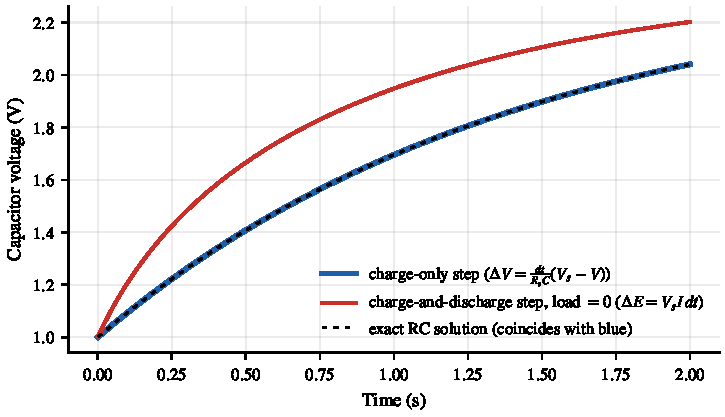
\includegraphics[width=0.78\linewidth]{fig_energy_accounting}
\caption{Zero-load charging from $\SI{1}{V}$: the charge-only step coincides with the exact RC solution; the charge-and-discharge step charges faster.}
\label{fig:energyaccounting}
\end{figure}
For the shipped demos the practical impact is small because the load dominates the active-state energy budget. Re-running the broadcast scenario ten times with a patched step that credits $V I_c\Delta t$ reduced the mean number of packets sent in $\SI{20}{s}$ from $124.4$ to $121.0$ ($\approx-2.7\%$). The effect would be larger for light loads or long active phases. Keep it in mind when interpreting duty-cycle numbers.
\end{reality}

\section{Chapter summary}
\begin{itemize}
 \item $C\,\dot V=(\Vs-V)/\Rs-V/\Rl-I_L$ gives $V(t)=V_\infty+(V_0-V_\infty)\e^{-t/\tau}$; $V_\infty=(\Vs-I_L\Rs)\Rl/(\Rl+\Rs)$; $\tau=(\Rs\parallel\Rl)C$.
 \item A node can sustain a current $I_{\max}=(\Vs-V)/\Rs-V/\Rl$; nodes whose typical load exceeds it must duty-cycle or starve.
 \item Amber advances the capacitor with a 1~ms hybrid step (exact leakage, Euler source). The charge-only step matches the exact solution to $2\times10^{-4}$~V.
 \item Hysteresis ($\Vhigh>\Vlow$) avoids chattering; $\Delta E=\tfrac12C(\Vhigh^2-\Vlow^2)=\SI{180}{\micro J}$ in the demos.
 \item Duty-cycle theorem: $D=P_{\mathrm{in}}/P_{\mathrm{act}}$.
 \item The active-mode step over-credits harvest by $\Vs/V$; $\approx3\%$ effect on demo packet counts.
\end{itemize}

\begin{codemap}
\small
\begin{tabularx}{\linewidth}{@{}>{\ttfamily}p{5.0cm}X@{}}
\toprule
\normalfont\bfseries Concept & \normalfont\bfseries Code (\file{amber/capacitor.py}, \file{controller.py})\\
\midrule
$R_s,R_l,C,\Delta t$ & \codew{CapacitorParams}\\
Eq.~\eqref{eq:chargestep} & \codew{Capacitor.capacitor_charging}\\
Leakage only & \codew{Capacitor.capacitor_selfdischarge}\\
Load only & \codew{Capacitor.load_discharging}\\
Charge + discharge & \codew{Capacitor.charge_and_discharge}\\
Clamp $\Vmax$ & \code{voltage_max}\\
Thresholds & \codew{VoltageThresholdsV(high, low)}\\
Who steps the capacitor & \codew{Controller.run}, via \codew{action.interrupt(cause)}\\
\bottomrule
\end{tabularx}
\end{codemap}

\section*{Exercises}
\begin{exercise}
For $\Rs=\SI{5}{k\ohm}$, $\Rl=\SI{100}{k\ohm}$, $C=\SI{200}{\micro F}$ (the SIC demo): compute $\tau$, and the time to charge from $0$ to $\SI{1.7}{V}$ with $\Vs=\SI{2.486}{V}$.
\end{exercise}
\begin{exercise}
A node draws a constant $\SI{300}{\micro A}$ while active. For what source voltages $\Vs$ is it energy-starved at $\Vlow=\SI{1.3}{V}$ (use $V_\infty<\Vlow$ with the load included)?
\end{exercise}
\begin{exercise}
Compute $\Delta E$ for $C=\SI{200}{\micro F}$, $\Vhigh=\SI{1.7}{V}$, $\Vlow=\SI{1.3}{V}$. By what factor must $C$ change to double the usable window? What if instead $\Vlow$ were lowered to $\SI{1.1}{V}$?
\end{exercise}
\begin{exercise}
Derive Eq.~\eqref{eq:tth} and verify the entry $t=\SI{3.37}{s}$ for Node~1 ($\Vs=\SI{1.971}{V}$).
\end{exercise}
\begin{exercise}
A node harvests $P_{\mathrm{in}}=\SI{200}{\micro W}$ into its capacitor and, while active, draws $\SI{4}{mW}$. What is its long-run duty cycle? Using the energy window $\Delta E=\SI{180}{\micro J}$, estimate $T_c$, $T_a$ and the number of active bursts per second.
\end{exercise}
\begin{exercise}
Show that the maximum of $V(\Vs-V)/\Rs$ over $V$ is $\Vs^2/(4\Rs)$, and use this to explain why the model never delivers more than $25\%$ of the nominal harvested power.
\end{exercise}

\part{Sharing the Medium}

\chapter{Random Access: From ALOHA to Framed Slots}
\label{ch:aloha}

\begin{defbox}[In this chapter you will learn]
\begin{itemize}
 \item why devices that cannot listen before they talk need \emph{random access};
 \item how to derive the throughput of pure and slotted ALOHA from the Poisson model;
 \item \emph{framed} slotted ALOHA, the scheme used by RFID readers and by Amber's registration and custom protocols: expected idle, success and collision slots, and the optimal frame size;
 \item how a reader can estimate the number of contenders and adapt its frame (Schoute, EPC Gen2's $Q$-algorithm), and how Amber's custom demo does it;
 \item why an \emph{energy-limited} network wants different parameters from a throughput-limited one, and how subcarrier shifts multiply capacity.
\end{itemize}
\end{defbox}

\section{The problem: many talkers, one channel}
\label{sec:aproblem}

A base station illuminates, say, a hundred nodes. When it asks ``who is there?'',
every node would like to answer at once; all answers share the same carrier. If two
reflections overlap in time on the same frequency they interfere, and (unless capture or
interference cancellation rescues them; Chapter~\ref{ch:sic}) neither is decoded.

The classical remedies are \emph{scheduling} (the base station assigns each node a
slot) and \emph{random access} (each node picks a slot by itself). Scheduling needs the
base station to know who exists; discovering who exists is precisely the problem. Hence
random access. For a battery-free node there is a second reason: \emph{it cannot
sense the channel}. Carrier-sense multiple access (CSMA), the workhorse of Wi-Fi, requires
a receiver that is awake and sensitive before every transmission---far beyond a
microwatt budget. So the only practical rule is \emph{``transmit once, at a random time
the reader has authorised''}.

\section{Pure ALOHA}
\label{sec:pure}

Norman Abramson's ALOHA system \citep{abramson1970} let radio terminals in Hawaii
transmit whenever they liked. Model it as follows. Packets have duration $T$. New
transmission attempts form a Poisson process with an average of $g$ attempts per
packet time (the \emph{offered load}). A packet starting at time $t_0$ is successful
if no other packet starts in the \emph{vulnerable interval} $(t_0-T,\,t_0+T)$, which has
length $2T$. For a Poisson process the probability of no arrival in an
interval of length $2T$ is $\e^{-2g}$. Throughput (successes per packet time) is
\begin{equation}
 s_{\mathrm{pure}}(g)=g\,\e^{-2g},\qquad s_{\max}=\frac{1}{2\e}\approx0.184\ \text{at}\ g=\tfrac12.
\end{equation}

\section{Slotted ALOHA}
\label{sec:slotted}

If time is divided into slots of length $T$ and everyone must start at a slot boundary, two packets collide
only if they choose the \emph{same} slot. The vulnerable interval shrinks to
$T$, and
\begin{equation}
 s_{\mathrm{slot}}(g)=g\,\e^{-g},\qquad s_{\max}=\frac1{\e}\approx0.368\ \text{at}\ g=1.
\label{eq:slotted}
\end{equation}
Synchronisation doubles the efficiency \citep{roberts1975}.

\begin{figure}[t]
\centering
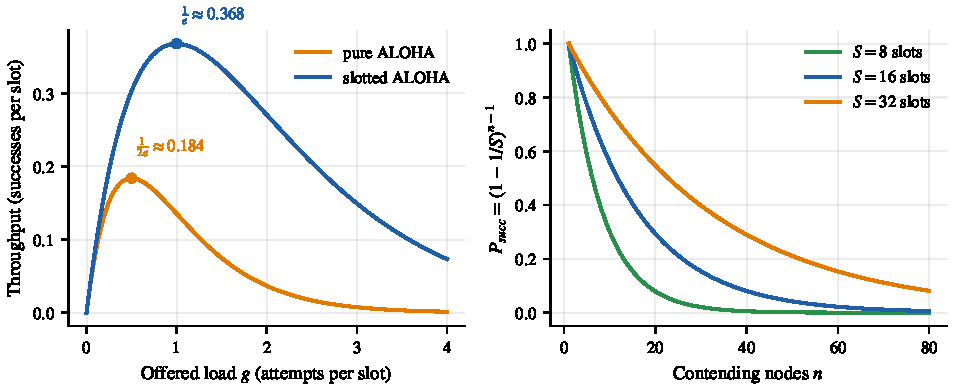
\includegraphics[width=0.95\linewidth]{fig_aloha}
\caption{Left: throughput of pure and slotted ALOHA. Right: the success probability of a single node in a frame of $S$ slots when $n$ nodes contend (Eq.~\eqref{eq:psucc}).}
\label{fig:aloha}
\end{figure}

\begin{intuition}[Why does the curve fall for large $g$?]
Throughput $=$ load $\times$ probability of success. Raising the load first
helps (more attempts) and then hurts (each attempt is more likely to collide). The maximum balances the two at $g=1$: on average exactly one attempt per slot.
\end{intuition}

\section{Framed slotted ALOHA}
\label{sec:fsa}

RFID readers, and Amber's registration, use \emph{framed} slotted ALOHA (FSA). The
base station announces a \emph{frame} of $S$ slots; each of the $n$ contending
nodes picks one slot uniformly at random and answers there. Because the number of
nodes is finite and they choose independently, the analysis is a balls-into-bins problem.

\paragraph{Slot statistics.}
The number of nodes in a given slot is Binomial$(n,1/S)$. Hence
\begin{align}
 \Pr[\text{slot idle}]&=\Big(1-\tfrac1S\Big)^{n},\\
 \Pr[\text{slot has exactly one node}]&=\frac nS\Big(1-\tfrac1S\Big)^{n-1},\\
 \Pr[\text{collision}]&=1-\text{(the two above)}.
\end{align}
The expected numbers of idle, successful and collision slots in a frame are
\begin{equation}
 E_0=S\Big(1-\tfrac1S\Big)^{n},\qquad E_1=n\Big(1-\tfrac1S\Big)^{n-1},\qquad E_c=S-E_0-E_1,
\label{eq:fsaexp}
\end{equation}
and a single node succeeds with probability
\begin{equation}
 P_{\mathrm{succ}}=\Big(1-\tfrac1S\Big)^{n-1}\;\approx\;\e^{-n/S}
\label{eq:psucc}
\end{equation}
(nobody else chose its slot). The \emph{slot efficiency} is
\begin{equation}
 \eta_S=\frac{E_1}{S}=\frac nS\Big(1-\tfrac1S\Big)^{n-1}\;\xrightarrow{S\to\infty}\;\frac nS\,\e^{-n/S}.
\end{equation}
Maximising over $S$ gives the \textbf{optimal frame size $S=n$}, with efficiency
$\approx1/\e=0.368$. Figure~\ref{fig:frameeff} shows the curves.

\begin{figure}[t]
\centering
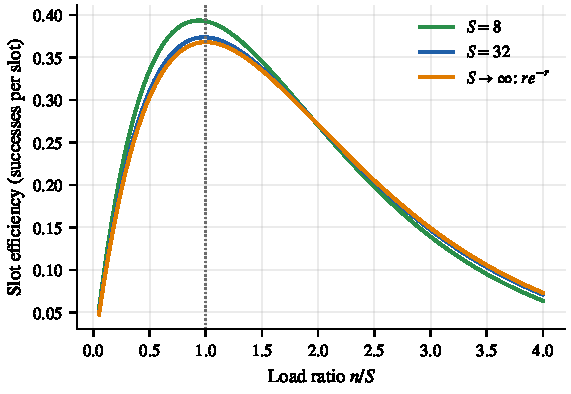
\includegraphics[width=0.58\linewidth]{fig_frame_efficiency}
\caption{Slot efficiency of framed slotted ALOHA against the load ratio $n/S$. All curves peak near $n/S=1$ at about $0.37$--$0.39$; the $S\to\infty$ limit is $re^{-r}$.}
\label{fig:frameeff}
\end{figure}

\begin{example}[A frame with 20 nodes and 16 slots]
By Eq.~\eqref{eq:fsaexp}: $E_0=16(15/16)^{20}=4.40$ idle slots; $E_1=20(15/16)^{19}=5.87$ successes; $E_c=5.73$ collision slots; efficiency $5.87/16=0.367$. Each node succeeds with probability $(15/16)^{19}=0.293$. Roughly seven of the twenty nodes are \emph{not} served in this frame, and a second frame is needed for them.
\end{example}

\paragraph{Multi-frame inventory.}
In an inventory the reader repeats frames until every node is identified. Suppose it could always
choose $S=n_k$, the number of nodes still unidentified. A frame then identifies
$E_1=n_k(1-1/n_k)^{n_k-1}\approx n_k/\e$ of them in expectation, so
\[
 n_{k+1}\approx n_k\Big(1-\tfrac1{\e}\Big)=0.63\,n_k,
\]
and the unidentified population decays geometrically. Going from $n=100$ to below one node takes
$\ln100/\ln(1/0.632)\approx10$ frames. The practical lesson is that \emph{the right frame size shrinks as nodes are identified}, so the reader has to keep estimating $n_k$.

\section{Estimating the number of contenders}
\label{sec:estimate}

The reader observes only the \emph{outcome} of each slot: idle ($c_0$ of them), success ($c_1$) or
collision ($c_c$). Schoute \citep{schoute1983} showed that at the optimal operating point a collision slot holds on average $2.39$ nodes, giving the estimate
\begin{equation}
 \hat n=c_1+2.39\,c_c.
\end{equation}
A simple lower bound is $n\ge c_1+2c_c$. EPC's Gen2 standard \citep{epcgen2} implements a variant of dynamic framing
through its \emph{$Q$-algorithm}: the frame has $2^Q$ slots and the reader adjusts a floating-point $Q_{fp}$ by
$\pm C$ after each collision (increase) or idle (decrease) slot.

\paragraph{Amber's custom protocol.}
The shipped \codew{custom_protocol} demo implements an adaptive FSA in the spirit of the
$Q$-algorithm (its docstring says ``EPC-Gen2 Q-algorithm style''). After each frame the base station
\begin{enumerate}
 \item counts $\text{heard}$ (decoded replies) and $\text{collided}$ (replies lost to collisions) and
   forms the number of contenders $m=\text{heard}+\text{collided}$ (each transmission increments exactly one of
   the two counters);
 \item smooths it, $\ell\leftarrow0.75\,\ell+0.25\,m$;
 \item sets a target frame size $\min\{32,\max\{2,\mathrm{round}(2\ell)\}\}$ and moves the actual frame size \emph{one slot} toward it, with a one-slot dead band above the target.
\end{enumerate}
Two comments. First, the base station here knows $m$ \emph{exactly}, because the simulator logs every colliding
packet individually; a real reader sees only that a slot collided (and would estimate $n$ with Schoute's formula).
This is an idealisation. Second, the target $S=2\ell$ is not the throughput-optimal $S=n$; the next section shows why that
can be a good choice here.

\section{An energy-aware twist}
\label{sec:energytwist}

In RFID a collision wastes \emph{airtime}. In an Ambient IoT node it also wastes \emph{joules}:
the node has already paid for the transmission. With the demo's numbers, a transmission
costs about $E_{\mathrm{tx}}\approx\SI{112}{\micro J}$ (Chapter~\ref{ch:controller}). The expected energy per \emph{successfully delivered} packet is
\begin{equation}
 \bar E_{\mathrm{deliv}}=\frac{E_{\mathrm{tx}}}{P_{\mathrm{succ}}}=\frac{E_{\mathrm{tx}}}{(1-1/S)^{n-1}}.
\end{equation}
\begin{center}
\small
\renewcommand{\arraystretch}{1.1}
\begin{tabular}{@{}lrrr@{}}
\toprule
$n=30$ nodes & slot efficiency & $P_{\mathrm{succ}}$ & energy per delivered packet\\
\midrule
$S=n=30$ & $0.374$ & $0.374$ & $\SI{299}{\micro J}$\\
$S=2n=60$ & $0.307$ & $0.614$ & $\SI{182}{\micro J}$\\
\bottomrule
\end{tabular}
\end{center}
Doubling the frame costs about $18\%$ of slot efficiency but cuts the energy spent per delivered packet by $39\%$.
\begin{keyidea}
A frame-size policy that is optimal for \emph{airtime} is not optimal for \emph{energy}. When every transmission
drains a scarce capacitor, a larger frame ($S>n$) is worth its idle slots. This is exactly the trade-off that Amber lets you explore, and a reason the
demo's rule-of-thumb $S\approx2\ell$ is sensible.
\end{keyidea}
There is a second coupling: the \emph{effective} $n$ is the number of nodes that are \emph{awake} when the frame is announced, which varies with their capacitors. The base station cannot observe that number (Chapter~\ref{ch:protocols}).

\section{Several orthogonal channels: subcarrier shifts}

With $K$ mutually orthogonal subcarrier shifts (Chapter~\ref{ch:backscatter}) and nodes spread evenly over them, collisions occur only among nodes with the same shift. Each group of
$n/K$ nodes runs an independent FSA in the same $S$ time slots, so the per-node success probability is $(1-1/S)^{n/K-1}$. If instead each node picked its
(slot, shift) pair uniformly at random, the number of independent resources would be $KS$ and
$P_{\mathrm{succ}}=(1-1/(KS))^{n-1}\approx\e^{-n/(KS)}$: the same to first order. Shifts and slots are
interchangeable currencies: $K$ shifts of $S$ slots give the collision behaviour of $KS$ slots at the
airtime cost of $S$. For $n=60$, $S=10$, $K=3$ the success probability is $(1-1/30)^{59}=0.135$.

\section{From the model to the simulator}

Amber reproduces the framed structure literally. The base station's schedule is a list of
RX windows, \emph{each window being one slot}; a node chooses \codew{random.randint(0, len(rx_slots)-1)}, uniformly, among the slots advertised
(Chapter~\ref{ch:bsmodule}). Three simulator details modify the textbook picture and will be analysed in Chapters~\ref{ch:sic} and~\ref{ch:bsengine}:
\begin{enumerate}
 \item the base station advertises the slots of the \emph{current and the next} frame, so only about half of the contenders
   can answer in a given frame;
 \item two nodes in the same slot collide only if they transmit within a $\SI{5}{ms}$ \emph{time window} of each other
   (they are not forced to transmit at the slot start), and only if they share a subcarrier shift;
 \item capture and SIC resolve some collisions that the classical model counts as lost.
\end{enumerate}
All three make Amber \emph{more optimistic} than Eq.~\eqref{eq:psucc} for the \emph{collision} aspect, and the first makes it \emph{slower} per frame.

\section{Chapter summary}
\begin{itemize}
 \item Battery-free nodes cannot carrier-sense, so the reader must authorise random-access slots.
 \item Pure ALOHA peaks at $1/(2e)\approx0.184$, slotted ALOHA at $1/e\approx0.368$.
 \item Framed slotted ALOHA: $E_1=n(1-1/S)^{n-1}$, $P_{\mathrm{succ}}=(1-1/S)^{n-1}\approx\e^{-n/S}$, optimum $S=n$.
 \item Schoute's estimator $\hat n=c_1+2.39\,c_c$ underlies adaptive framing; Amber's custom demo uses its own exact counts.
 \item For energy-limited tags a larger frame ($S\approx2n$) can minimise energy per delivered packet.
 \item $K$ orthogonal subcarrier shifts act like $K$ times as many slots.
\end{itemize}

\begin{codemap}
\small
\begin{tabularx}{\linewidth}{@{}>{\ttfamily}p{5.2cm}X@{}}
\toprule
\normalfont\bfseries Concept & \normalfont\bfseries Code\\
\midrule
Random slot choice & \codew{BackscatterModule.handle_command} (\codew{random.randint})\\
Frame = TX command + $S$ RX windows & schedule entries \code{("tx",...)}, \code{("rx",...)} in \file{bsengine.py}\\
Adaptive frame size & \codew{adaptive_aloha_policy} in \file{custom_protocol_demo.py}\\
Contender count & \codew{decoded_this_frame}, \codew{total_collided}\\
\bottomrule
\end{tabularx}
\end{codemap}

\section*{Exercises}
\begin{exercise}
Derive the pure-ALOHA throughput and its maximum. Why is the vulnerable period twice as long as in the slotted case?
\end{exercise}
\begin{exercise}
For $n=20$ nodes and $S=16$ slots compute $E_0$, $E_1$, $E_c$ and the efficiency (verify the worked example). How many slots would maximise efficiency, and what would it be?
\end{exercise}
\begin{exercise}
After a frame of $S=16$ slots the reader observes $c_0=6$, $c_1=5$, $c_c=5$. Estimate the number of contenders using Schoute's formula and the lower bound. Which frame size should it use next?
\end{exercise}
\begin{exercise}
Compute the energy per delivered packet for $n=30$ and $S\in\{30,45,60,90\}$ when $E_{\mathrm{tx}}=\SI{112}{\micro J}$ and compare with the slot efficiency. Where would you set the frame size if idle slots cost nothing but airtime counts against latency?
\end{exercise}
\begin{exercise}
$n=60$ nodes are divided equally among $K=3$ subcarrier shifts and all reply in a frame of $S=10$ slots. Compute the per-node success probability, and compare with $K=1$.
\end{exercise}

\chapter{Capture, SINR and Successive Interference Cancellation}
\label{ch:sic}

\begin{defbox}[In this chapter you will learn]
\begin{itemize}
 \item the \emph{physical} (SINR-threshold) model of a collision and the \emph{capture effect};
 \item the principle of \emph{successive interference cancellation} (SIC), why it works best when received powers differ, and how imperfect cancellation changes the SINR sequence;
 \item exactly how Amber groups, resolves and logs colliding packets, step by step;
 \item three behaviours of that pipeline that differ from textbook expectations, each verified by experiment, including a measured \emph{SIC on/off} ablation.
\end{itemize}
\end{defbox}

\section{From ``collision'' to SINR}
\label{sec:physmodel}

Chapter~\ref{ch:aloha} treated a collision as a binary event: if two packets share a
slot, both are lost. This is the \emph{protocol model}. Real receivers are more
forgiving. A packet can be decoded despite overlapping with another if it is
\emph{strong enough} relative to everything else. This is the \emph{physical model}: packet $i$ is
decoded if its signal-to-interference-plus-noise ratio
\begin{equation}
 \gamma_i=\frac{P_i}{\sum_{j\ne i}P_j+N}\ \ge\ \gamma_{\mathrm{req}}.
\label{eq:sinrdef}
\end{equation}
The threshold $\gamma_{\mathrm{req}}$ is a single number that stands in for the modulation, coding and
receiver design (Amber's default in the base station is $3$~dB).

\paragraph{The capture effect.}
When two packets collide and one is much stronger, the receiver locks onto it and ignores the other. Roberts called this
\emph{capture} \citep{roberts1975}. For two packets of power $P_1\ge P_2$ and negligible noise, capture requires
\[
 \frac{P_1}{P_2}\ge\gamma_{\mathrm{req}}
 \quad\Longleftrightarrow\quad
 (P_1-P_2)_{\mathrm{dB}}\ge(\gamma_{\mathrm{req}})_{\mathrm{dB}}.
\]
Noise changes this when the weaker packets are near the noise floor, as Figure~\ref{fig:sinrgap} shows: a strong
pair ($-60$~dBm) is interference-limited and the SINR grows without bound with the gap; a weak pair ($-80$~dBm)
is noise-limited and saturates at about $8$~dB no matter how small the interferer.

\begin{figure}[t]
\centering
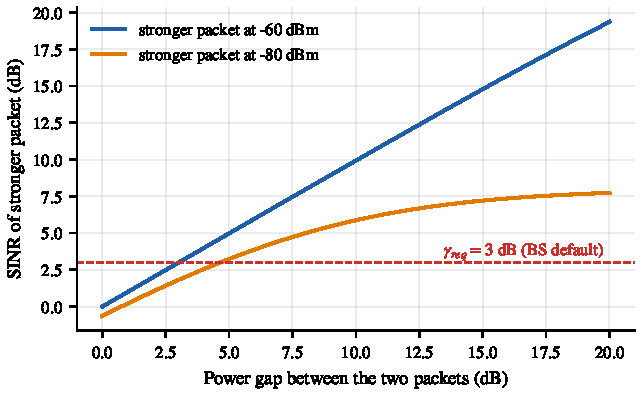
\includegraphics[width=0.62\linewidth]{fig_sinr_vs_gap}
\caption{SINR of the stronger of two colliding packets against the power gap, for thermal noise $\SI{-88}{dBm}$. At $-60$~dBm the curve is interference-limited; at $-80$~dBm it saturates because noise dominates. The dashed line is Amber's default requirement of $3$~dB.}
\label{fig:sinrgap}
\end{figure}

\paragraph{Why capture matters for backscatter.}
In Chapter~\ref{ch:backscatter} we saw that the uplink loses $2\times10\,n\log_{10}d$~dB: for a pair of
nodes whose distances differ by a factor of $2$, the received powers differ by
$2\cdot22\log_{10}2=\SI{13.2}{dB}$ below the UMa breakpoint and $2\cdot40\log_{10}2=\SI{24.1}{dB}$ beyond it. This
\emph{near--far diversity} makes capture frequent: random placement itself supplies power differences.

\section{Successive interference cancellation}
\label{sec:sictheory}

\subsection{The principle}

Capture decodes the strongest packet and discards the rest. But the others
may be perfectly decodable \emph{once the strongest is out of the way}. SIC makes this explicit \citep{tse2005,cover2006}:
\begin{enumerate}
 \item sort the received signals by power;
 \item decode the strongest, treating all others (and noise) as interference;
 \item if decoding succeeded, \emph{reconstruct and subtract} that signal from the received waveform;
 \item repeat on the remainder; stop at the first failure.
\end{enumerate}
In information theory, SIC with ideal cancellation achieves the corner points of the multiple-access capacity region,
which is why it is considered the receiver of choice in non-orthogonal multiple access (NOMA).

\subsection{The SINR sequence}

Let the powers sorted in decreasing order be $P_{(1)}\ge P_{(2)}\ge\dots\ge P_{(m)}$ and let $\varepsilon\in[0,1]$ be the fraction of an
already-decoded signal that is \emph{not} removed ($\varepsilon=0$: perfect cancellation). When decoding the $k$-th strongest,
\begin{equation}
 \gamma_{(k)}=\frac{P_{(k)}}{\displaystyle\sum_{j>k}P_{(j)}+\varepsilon\sum_{j<k}P_{(j)}+N}.
\label{eq:sicsinr}
\end{equation}
With perfect cancellation only \emph{weaker} packets interfere. A useful design rule follows: if successive powers
decrease by a constant ratio $\rho$ and noise is negligible, the SINR of every stage is
$1/(\rho^{-1}+\rho^{-2}+\cdots)=\rho-1$, so SIC decodes all packets iff $\rho\ge1+\gamma_{\mathrm{req}}$.
\emph{Each packet must be stronger than the sum of all weaker ones by the decoding threshold.}
For $\gamma_{\mathrm{req}}=3$~dB this means $\rho\ge3$ ($4.8$~dB) between neighbours.

\begin{figure}[t]
\centering
\begin{tikzpicture}[x=1cm,y=1cm,scale=0.92]
 \def\u{4.0}
 % powers (linear, relative to P1): 1, 0.316, 0.1, 0.0016
 % ---- column 1: all packets present
 \begin{scope}[shift={(0,0)}]
  \draw[fill=agrey!50] (0,0) rectangle (1.4,0.02);
  \draw[fill=agreen!70] (0,0.02) rectangle (1.4,0.42);
  \draw[fill=aorange!70] (0,0.42) rectangle (1.4,1.69);
  \draw[fill=ablue!75,line width=1.4pt] (0,1.69) rectangle (1.4,5.69);
  \node[white,font=\sffamily\small] at (0.7,3.7) {$P_1$};
  \node[font=\sffamily\scriptsize] at (0.7,1.05) {$P_2$};
  \node[font=\sffamily\scriptsize] at (0.7,0.22) {$P_3$};
  \draw[decorate,decoration={brace,amplitude=4pt}] (1.5,1.69) -- (1.5,0) node[midway,right=5pt,font=\sffamily\scriptsize,align=left] {interference\\$P_2{+}P_3{+}N$};
  \node[font=\sffamily\scriptsize,align=center] at (0.7,-0.75) {\textbf{step 1}: decode $P_1$\\ $\gamma_1=3.79$~dB $\ge3$ \checkmark};
 \end{scope}
 % ---- column 2: P1 removed
 \begin{scope}[shift={(5.6,0)}]
  \draw[fill=agrey!50] (0,0) rectangle (1.4,0.02);
  \draw[fill=agreen!70] (0,0.02) rectangle (1.4,0.42);
  \draw[fill=aorange!70,line width=1.4pt] (0,0.42) rectangle (1.4,1.69);
  \draw[dashed,agrey] (0,1.69) rectangle (1.4,5.69);
  \node[agrey,font=\sffamily\scriptsize,align=center] at (0.7,3.7) {$P_1$ decoded\\and subtracted};
  \node[font=\sffamily\scriptsize] at (0.7,1.05) {$P_2$};
  \node[font=\sffamily\scriptsize] at (0.7,0.22) {$P_3$};
  \draw[decorate,decoration={brace,amplitude=3pt}] (1.5,0.42) -- (1.5,0) node[midway,right=5pt,font=\sffamily\scriptsize,align=left] {$P_3{+}N$};
  \node[font=\sffamily\scriptsize,align=center] at (0.7,-0.75) {\textbf{step 2}: decode $P_2$\\ $\gamma_2=4.93$~dB \checkmark};
 \end{scope}
 % ---- column 3
 \begin{scope}[shift={(11.2,0)}]
  \draw[fill=agrey!50] (0,0) rectangle (1.4,0.02);
  \draw[fill=agreen!70,line width=1.4pt] (0,0.02) rectangle (1.4,0.42);
  \draw[dashed,agrey] (0,0.42) rectangle (1.4,1.69);
  \draw[dashed,agrey] (0,1.69) rectangle (1.4,5.69);
  \node[font=\sffamily\scriptsize] at (0.7,0.22) {$P_3$};
  \draw[decorate,decoration={brace,amplitude=2pt}] (1.5,0.02) -- (1.5,0) node[midway,right=3pt,font=\sffamily\scriptsize] {$N$};
  \node[font=\sffamily\scriptsize,align=center] at (0.7,-0.75) {\textbf{step 3}: decode $P_3$\\ $\gamma_3=17.98$~dB \checkmark};
 \end{scope}
\end{tikzpicture}
\caption{SIC on three colliding packets at $-60$, $-65$ and $-70$~dBm with a $\SI{-88}{dBm}$ noise floor and $\gamma_{\mathrm{req}}=3$~dB. Bar heights are \emph{linear} power. Without cancellation only the strongest would be decoded (capture); with SIC all three are.}
\label{fig:sicsteps}
\end{figure}

\begin{example}[Three packets, with and without SIC]
Powers $-60,-65,-70$~dBm, i.e.\ $1.00,\,0.316,\,0.100$~nW, noise $1.59$~pW. Step~1: $\gamma_1=1/(0.316+0.100+0.0016)=2.39=\SI{3.79}{dB}\ge3$, decoded.
After removal, step~2: $\gamma_2=0.316/(0.100+0.0016)=3.11=\SI{4.93}{dB}$, decoded. Step~3: $\gamma_3=0.100/0.0016=62.8=\SI{17.98}{dB}$, decoded. All three succeed;
capture alone would deliver only the first. If the packets were $-60$ and $-63$~dBm, $\gamma_1=\SI{2.99}{dB}<3$: \emph{nothing} is decoded, a razor-edge illustrating how sharp the threshold model is.
With $10\%$ residual ($\varepsilon=0.1$) step~2 becomes $\gamma_2=0.316/(0.100+0.0016+0.1\cdot1.0)=1.57=\SI{1.96}{dB}<3$: the second packet is \emph{lost}. SIC is very sensitive to cancellation quality.
\end{example}

\section{How Amber resolves collisions}
\label{sec:ambercollisions}

The base station resolves collisions at the \emph{end of each RX window}. Algorithm~\ref{alg:rxbuffer} states the procedure in plain steps; we then explain each design choice.

\begin{algorithm}[t]
\caption{Processing of one RX window (\code{BSBehavior._process_rx_buffer})}
\label{alg:rxbuffer}
\begin{algorithmic}[1]
\Require buffer $\mathcal B$ of arrivals $(t_i,\mathrm{node}_i,P_i,\mathrm{sector}_i,c_i)$ collected during this window; noise $N$; $\gamma_{\mathrm{req}}$
\State group the arrivals by subcarrier shift $c$
\For{each shift group $\mathcal G$}
  \State sort $\mathcal G$ by arrival time; $\mathrm{used}\gets\emptyset$; $\mathrm{coll}\gets[\,]$
  \For{each packet $i$ in time order, $i\notin\mathrm{used}$}
     \State $\mathcal C\gets\{i\}\cup\{j\notin\mathrm{used},\,j\ne i:\ |t_i-t_j|\le\SI{5}{ms}\}$
     \State \textbf{if} $|\mathcal C|>1$ \textbf{then} append $\mathcal C$ to $\mathrm{coll}$ \textbf{end if}; \quad $\mathrm{used}\gets\mathrm{used}\cup\mathcal C$
  \EndFor
  \For{each collision group $\mathcal C$ in $\mathrm{coll}$}
     \State $\mathrm{dec}\gets$ \Call{SIC}{powers of $\mathcal C$, $N$, $\gamma_{\mathrm{req}}$}
     \State \textbf{if} SIC is disabled \textbf{then} $\mathrm{dec}\gets$ first element of $\mathrm{dec}$ \textbf{end if} \Comment{capture only}
  \EndFor
  \For{each packet $p\in\mathcal G$}
     \State $\mathrm{collided}\gets(p\ \text{is in a collision group})\wedge(p\notin\mathrm{dec})$
     \State \textbf{skip} $p$ if its sector index is invalid or $P_p<$ sensitivity of its sector
     \State log \code{RxPacket}$(\dots,\mathrm{collided})$; update counters
     \State \textbf{if not} collided \textbf{then} record node as decoded; queue an ACK if new \textbf{end if}
  \EndFor
\EndFor
\end{algorithmic}
\end{algorithm}

\begin{algorithm}[t]
\caption{SIC as implemented (\code{packet_analysis.apply_sic})}
\label{alg:sic}
\begin{algorithmic}[1]
\Require powers $P_i$ (W), noise $N$, $\gamma_{\mathrm{req}}$, cancellation factor $\kappa$
\State $R_i\gets P_i$; $\mathrm{cand}\gets$ all packets; $\mathrm{dec}\gets[\,]$
\While{$\mathrm{cand}\ne\emptyset$}
  \State $k\gets\arg\max_{i\in\mathrm{cand}}R_i$
  \State $\gamma_k\gets R_k/\big(\sum_{j\in\mathrm{cand},j\ne k}R_j+N\big)$
  \If{$\gamma_k\ge\gamma_{\mathrm{req}}$}
     \State append $k$ to $\mathrm{dec}$; remove $k$ from $\mathrm{cand}$; $R_k\gets(1-\kappa)P_k$ \Comment{residual stored, but never summed again}
  \Else \ \textbf{break}
  \EndIf
\EndWhile
\State \Return $\mathrm{dec}$
\end{algorithmic}
\end{algorithm}

\paragraph{Design choice 1: the buffer is per RX window.}
Each \codew{("rx", d, id)} schedule entry is a separate window, and the buffer is cleared at its start. Consequently \emph{packets in different windows never collide}: a window is one \emph{slot} in the sense of Chapter~\ref{ch:aloha}.

\paragraph{Design choice 2: collision means time-proximity, not overlap.}
A simulated backscatter packet has no duration in the buffer---it is a point event at the instant of transmission. The simulator
therefore declares two packets to collide if they are within $\SI{5}{ms}$ of each other (the \codew{collision_window_ms} argument).
Within one slot of \SIrange{8}{15}{ms}, two nodes that choose the same slot but start $\SI{6}{ms}$ apart (for instance
because one was still in its \emph{processing} state when the slot opened) do \emph{not} collide.

\paragraph{Design choice 3: the group is built greedily.}
For each unused packet $i$, the group consists of $i$ and \emph{all unused packets within $5$~ms of $i$}. This is a greedy neighbourhood, not transitive clustering.
We tested arrivals at $10,14,18$~ms: packets at $10$ and $14$ form a group and collide, but the packet at $18$ ($4$~ms from the second one, $8$~ms from the first) is \emph{not} in it and is decoded
as a lone packet. Exercise~\ref{ex:greedy} asks you to find the logic.

\paragraph{Design choice 4: capture-only without SIC.}
With SIC off the base station runs the same routine with $\kappa=0$ and keeps only the first decoded packet (the strongest, if its SINR
passes). So ``SIC off'' means \emph{capture only}, ``SIC on'' means \emph{every packet that passes the successive test is kept}.

\paragraph{Design choice 5: subcarriers are perfectly orthogonal.}
Packets with different \codew{subcarrier_shift} values are placed in different groups and \emph{cannot} collide, as discussed in Chapter~\ref{ch:backscatter}.

\begin{reality}[Three things the pipeline does that you might not expect]
\textbf{(1) The cancellation factor is inert.} The \code{apply_sic} docstring explains that $\kappa=0.9$ leaves $10\%$ of a decoded signal as residual interference. In the
implementation (Algorithm~\ref{alg:sic}, line~7) the residual $(1-\kappa)P_k$ is stored, but the decoded packet has just been removed from the candidate set, and interference is summed
only over candidates; the residual is never used. We confirmed this by running \code{apply_sic} on several power sets with $\kappa\in\{0,0.5,0.9,0.99,1\}$: the decoded sets were \emph{identical in every case}. Amber's ``SIC'' is therefore
\emph{perfect} cancellation; imperfect cancellation (Eq.~\eqref{eq:sicsinr} with $\varepsilon>0$) is not simulated. The fix would be a one-line change
that adds the residuals of already-decoded packets to the interference sum.

\textbf{(2) A lone packet bypasses the SNR test.} The noise power enters \emph{only} the SINR computation of colliding groups. A single packet that passes the sector's sensitivity gate is logged as decoded regardless of its SNR. We injected a packet at $\SI{-105}{dBm}$
(SNR $=-17$~dB against $\SI{-88}{dBm}$ of noise) and it was decoded.

\textbf{(3) Sub-sensitivity packets still interfere.} The sensitivity filter is applied \emph{after} the SIC decision, so a packet below the sector's sensitivity is dropped from the log but still counted as an interferer for the packets around it.
\end{reality}

\section{Does SIC matter? A controlled experiment}
\label{sec:sicexperiment}

The two shipped broadcast demos differ in \emph{six} ways at once: \code{enable_sic}, capacitance ($300\to\SI{200}{\micro F}$), RX slot length
($10\to\SI{15}{ms}$), slots per frame ($2\to3$), sector beamwidth ($65^\circ\to30^\circ$) and sector sensitivity ($-100\to\SI{-80}{dBm}$). Their results therefore cannot isolate the effect of SIC. We rebuilt the scenario with a single function
and varied the factors one at a time over ten random seeds (script \file{textbook/code/sic_ablation.py}). Table~\ref{tab:sicablation} shows the result.

\begin{table}[t]
\centering
\small
\caption{Delivery error rate (DER $=1-\text{decoded}/\text{sent}$) and throughput of the 3-node broadcast scenario over $\SI{20}{s}$, mean over $10$ seeds (standard deviation of DER in brackets).}
\label{tab:sicablation}
\renewcommand{\arraystretch}{1.1}
\begin{tabular}{@{}lrrr@{}}
\toprule
Configuration & SIC & DER & Throughput (pkt/s)\\
\midrule
Broadcast demo parameters & off & $2.57\%$ ($0.85$) & $6.06$\\
Broadcast demo parameters & on & $0.00\%$ ($0.00$) & $6.22$\\
SIC-demo parameters & off & $2.89\%$ ($1.61$) & $6.41$\\
SIC-demo parameters & on & $0.00\%$ ($0.00$) & $6.60$\\
\midrule
\multicolumn{4}{@{}l}{\emph{One factor changed from the broadcast demo (SIC off)}}\\
Capacitance $\SI{200}{\micro F}$ & off & $2.36\%$ ($0.71$) & $6.80$\\
RX slot $\SI{15}{ms}$ & off & $2.55\%$ ($1.18$) & $5.93$\\
$3$ slots & off & $2.12\%$ ($1.16$) & $5.99$\\
Beamwidth $30^\circ$ & off & $2.57\%$ ($0.85$) & $6.06$\\
Sector sensitivity $\SI{-80}{dBm}$ & off & $2.57\%$ ($0.85$) & $6.06$\\
\bottomrule
\end{tabular}
\end{table}

The conclusions are clean. (i) Enabling SIC removes \emph{all} delivery errors, from $\approx2.6$--$2.9\%$ to $0.00\%$, in both parameter sets. (ii) None of the other factors changes DER meaningfully; beamwidth and sector
sensitivity have \emph{exactly} the same value because all three nodes sit on the sector's boresight and far above $\SI{-80}{dBm}$. (iii) SIC raises throughput slightly
($\approx+2.6\%$) simply because the lost packets are recovered. The improvement shown by the shipped SIC demo is thus attributable to SIC itself.

\begin{example}[Why SIC rescues exactly these collisions]
The three demo nodes arrive at the base station with $-45.7$, $-49.7$ and $-68.7$~dBm. Node~0 against Node~1 alone: gap $4.0$~dB, so $\gamma_0=4.0$~dB$\ge3$: capture works for Node~0 and Node~1 is lost, unless SIC is on, when Node~1 is decoded next against only the noise. For all three together,
$\gamma_0=1/(0.395+0.005)=2.50=\SI{3.98}{dB}$, again passing, and the remaining two are separated by $19$~dB. Without SIC at most \emph{one} packet of any colliding group survives; with SIC \emph{all} do.
This near-perfect separation is an artefact of the nodes' very different distances and the perfect cancellation of the previous reality check; with equal-distance nodes SIC would help far less.
\end{example}

\section{What the threshold model abstracts away}

The SINR threshold $\gamma_{\mathrm{req}}$ replaces a lot of physics: the modulation and coding scheme, the receiver's ability to
\emph{lock onto a preamble} while another signal is present (capture in real receivers depends on arrival order and synchronisation),
the length of the overlap, and the decoding of partially overlapping packets. It is a good \emph{system-level} abstraction when one wants to compare
protocols, and a poor basis for predicting the absolute packet-error rate of a particular radio.

\begin{codemap}
\small
\begin{tabularx}{\linewidth}{@{}>{\ttfamily}p{5.0cm}X@{}}
\toprule
\normalfont\bfseries Concept & \normalfont\bfseries Code\\
\midrule
SINR, Eq.~\eqref{eq:sinrdef} & \code{apply_sic} (\file{packet_analysis.py})\\
Noise power & \codew{thermal_noise_watts}\\
Per-window buffer & \codew{BSBehavior._rx_buffer}, \code{_buffer_rx}\\
Grouping and resolution & \codew{BSBehavior._process_rx_buffer}\\
SIC on/off & \code{enable_sic} (constructor)\\
$\gamma_{\mathrm{req}}$ & \codew{required_sinr_db} (default $3$)\\
$\kappa$ & \codew{cancellation_factor} (default $0.9$; \emph{inert})\\
\bottomrule
\end{tabularx}
\end{codemap}

\section{Chapter summary}
\begin{itemize}
 \item The physical model decodes a packet iff its SINR exceeds $\gamma_{\mathrm{req}}$; capture follows when one packet is stronger by roughly $\gamma_{\mathrm{req}}$.
 \item SIC decodes packets in descending power order and removes each; all packets can be decoded if successive powers differ by a factor $\ge1+\gamma_{\mathrm{req}}$.
 \item Amber buffers packets per RX window, groups by subcarrier and a $5$~ms greedy proximity window, then applies SIC.
 \item Verified quirks: the cancellation factor has no effect (SIC is perfect), lone packets skip the SNR test, sub-sensitivity packets still interfere.
 \item In a controlled experiment SIC cut DER from $\approx2.6$--$2.9\%$ to $0\%$; other demo parameter changes had no effect.
\end{itemize}

\section*{Exercises}
\begin{exercise}
Two packets arrive at $-62$ and $-70$~dBm with noise $\SI{-88}{dBm}$ and $\gamma_{\mathrm{req}}=3$~dB. Compute both SINRs under SIC. Would capture alone decode the first? The second?
\end{exercise}
\begin{exercise}
Three equal packets at $-70$~dBm collide. What is the SINR of the first decoded packet? What does SIC do?
\end{exercise}
\begin{exercise}
For $\gamma_{\mathrm{req}}=3$~dB and negligible noise, how much stronger (in dB) must the strongest of four packets be than the weakest if consecutive powers are in a constant ratio and SIC is to decode all four?
\end{exercise}
\begin{exercise}\label{ex:greedy}
Four packets on one subcarrier arrive at $3,7,11,15$~ms. Apply Algorithm~\ref{alg:rxbuffer}: how many collision groups are formed and which packets are in them? How would transitive clustering differ?
\end{exercise}
\begin{exercise}
Recompute the example of Figure~\ref{fig:sicsteps} for $\varepsilon=0.05$ and $\varepsilon=0.1$ using Eq.~\eqref{eq:sicsinr}. Which packets are decoded in each case? Compare with what Amber's implementation would report.
\end{exercise}

\chapter{Protocols: Discovery, Registration and Polling}
\label{ch:protocols}

\begin{defbox}[In this chapter you will learn]
\begin{itemize}
 \item why Ambient IoT protocols are \emph{command-driven}, and the two-phase structure (discovery, then data collection) used by the paper;
 \item Amber's built-in protocol as a message sequence: \code{send_id}, random slot, backscattered ID, \code{ack}, \code{send_data};
 \item the trade-offs between \emph{broadcast} and \emph{unicast} polling, and why a well-scheduled network is usually \emph{energy-limited}, not airtime-limited;
 \item a mean-field model of registration success versus node density, compared with simulation;
 \item the problem of \emph{limited visibility}: what a base station cannot know.
\end{itemize}
\end{defbox}

\section{Command-driven networks}
\label{sec:cmddriven}

Every protocol in this book is \emph{reader-talks-first}, for the three reasons we met in earlier chapters:
\begin{enumerate}
 \item a passive node cannot afford a receiver that listens all the time, so commands are rare, explicit and short;
 \item a node can transmit only by reflecting a carrier, so it should transmit only when the reader says the carrier is on and a slot is open;
 \item the reader is the only entity that can coordinate: it has power, a clock and a view of the whole cell.
\end{enumerate}
The reader's repertoire is small: \emph{broadcast a command}, \emph{open reply windows (slots)}, \emph{acknowledge}. A node's repertoire is smaller still: \emph{if I heard a command and my slot is now, reflect my message}.

The paper describes the base stations of its experiment as operating \emph{in two phases}: ``a discovery phase, where nodes register by responding with their identifiers in random slots, followed by a data collection phase, where the base station periodically requests sensor readings from each registered node individually by its identifier.'' The first phase is framed slotted ALOHA (Chapter~\ref{ch:aloha}); the second is \emph{polling}.

\section{Amber's built-in protocol}
\label{sec:builtin}

The default protocol is implemented jointly by the node's \codew{BackscatterModule} and the base station's schedule. It has three commands:
\begin{center}
\small
\renewcommand{\arraystretch}{1.15}
\begin{tabularx}{\linewidth}{@{}>{\ttfamily}p{2.1cm}>{\raggedright}p{3.9cm}>{\raggedright\arraybackslash}X@{}}
\toprule
\normalfont\bfseries Command & \normalfont\bfseries Sent by base station & \normalfont\bfseries Node reaction\\
\midrule
send\_id & broadcast, with the list of upcoming RX slots & unless already registered: pick a slot at random; state $\to$ \emph{wait\_ack}\\
ack & in an ACK slot, to every node whose ID was decoded & if in \emph{wait\_ack}: state $\to$ \emph{registered}\\
send\_data & broadcast (\code{target=-1}) or to one node \code{target=i}; with RX slots & if registered (and addressed): choose a slot (random for broadcast, the first for unicast)\\
\bottomrule
\end{tabularx}
\end{center}
\noindent A node thus lives in three \emph{protocol states}: \emph{idle} (never heard a command), \emph{wait\_ack} (has chosen a slot to send its ID) and \emph{registered}.

\begin{figure}[t]
\centering
\begin{tikzpicture}[x=1cm,y=1cm]
 % lifelines
 \node[box,fill=lightorange,draw=aorange] (bs) at (0,0) {Base station};
 \node[box,fill=lightgreen,draw=agreen] (nd) at (9,0) {Node};
 \draw[dashed,agrey] (bs.south) -- ++(0,-9.4);
 \draw[dashed,agrey] (nd.south) -- ++(0,-9.4);
 % messages
 \draw[->,thick,ablue] (0,-1.0) -- node[above,lab]{\code{send_id} (broadcast) + RX slots} (9,-1.3);
 \node[lab,align=left,anchor=west] at (9.2,-1.55) {\emph{idle} $\to$ \emph{wait\_ack};\\random slot $r$};
 \draw[->,thick,aorange] (9,-2.8) -- node[above,lab,sloped]{backscatter ID in slot $r$} (0,-3.1);
 \node[lab,align=left,anchor=west] at (0.25,-3.55) {decode (capture / SIC);\\queue ACK};
 \draw[->,thick,ablue] (0,-4.5) -- node[above,lab]{\code{ack} (ACK slot)} (9,-4.8);
 \node[lab,align=left,anchor=west] at (9.2,-5.0) {\emph{wait\_ack} $\to$ \emph{registered}};
 \draw[->,thick,ablue] (0,-6.0) -- node[above,lab,sloped]{\code{send_data}(target$=i$) + next RX slot} (9,-6.3);
 \draw[->,thick,aorange] (9,-7.6) -- node[above,lab,sloped]{backscatter data in slot} (0,-7.9);
 \node[lab,align=left,anchor=west] at (0.25,-8.35) {data counted as received};
 \draw[decorate,decoration={brace,amplitude=5pt,mirror}] (-0.9,-0.8) -- (-0.9,-5.0) node[midway,left=2pt,lab,align=right]{discovery\\(random\\access)};
 \draw[decorate,decoration={brace,amplitude=5pt,mirror}] (-0.9,-5.8) -- (-0.9,-8.2) node[midway,left=2pt,lab,align=right]{data\\collection\\(polling)};
\end{tikzpicture}
\caption{Message sequence of Amber's default protocol for one node. The two phases correspond to those of the paper. In each phase the \emph{reply} is a backscatter packet inside an RX window the base station advertised in the command.}
\label{fig:msc}
\end{figure}

The sequence in Figure~\ref{fig:msc} has several details to appreciate.
\begin{itemize}
 \item Commands carry the \emph{timing of future RX windows}, so the node knows when its reply is permitted. The base station obtains this by \emph{looking ahead} in its schedule (Chapter~\ref{ch:bsengine}).
 \item An ACK is not itself a radio-simulated packet: it is a direct method call on every node whose ID was decoded. In a real system it would be a downlink message that could be lost.
 \item A node that is \emph{already registered} ignores \code{send_id}, which is what lets discovery converge: as more nodes register, fewer contend.
\end{itemize}

\section{Broadcast versus unicast polling}
\label{sec:bcvsuc}

Once nodes are registered, the base station collects data in one of two ways.

\paragraph{Broadcast.} One command \codew{send_data(target=-1)} followed by $S$ RX slots; each registered node picks a slot at random. This costs one command per frame, but the nodes contend: it is again FSA with $n$ contenders, with all the collisions of Chapter~\ref{ch:aloha}.

\paragraph{Unicast.} One command per node, \codew{send_data(target=i)}, each followed by the \emph{next} RX slot. Because only node $i$ is allowed to answer, there are \emph{no collisions}. The paper notes exactly this: ``No collisions occur during data collection since nodes are queried individually.'' The price is overhead: $N$ commands per round.

\begin{center}
\small
\renewcommand{\arraystretch}{1.15}
\begin{tabularx}{\linewidth}{@{}>{\sffamily\bfseries}p{3.0cm}XX@{}}
\toprule
 & Broadcast (FSA) & Unicast (polling)\\
\midrule
Commands per round & 1 & $N$\\
Collisions & yes, $P_{\mathrm{succ}}\approx\e^{-n/S}$ & none by construction\\
Airtime per round & $T_{\mathrm{cmd}}+S\,T_{\mathrm{slot}}$ & $N(T_{\mathrm{cmd}}+T_{\mathrm{slot}})$\\
Needs to know the nodes? & no & yes (IDs from discovery)\\
Wasted energy on collisions & yes & none\\
\bottomrule
\end{tabularx}
\end{center}

\subsection{Airtime is rarely the bottleneck}

Consider the shipped \code{unicast} demo: three nodes, each poll is $T_{\mathrm{cmd}}=\SI{5}{ms}$ plus a $\SI{10}{ms}$ slot, so a round takes $\SI{45}{ms}$. In $\SI{20}{s}$ the base station issues about $20\,001/45\times3\approx1333$ polls. The measured result is $125$ packets decoded: only \textbf{$\approx9\%$ of the polls are answered}. The other $91\%$ went to nodes that were \emph{not ready}: asleep recharging, or in a state other than \emph{wait\_slot}. The system is \emph{energy-limited}: throughput is set by how often the capacitors allow a node to transmit (we measured between $0.9$ and $2.8$ packets per second per node in the demos, Chapter~\ref{ch:capacitor}), not by how fast the base station can poll.

\begin{keyidea}[Energy, not airtime, limits throughput]
In a well-scheduled Ambient IoT network without collisions, delivered throughput is
\[
 \text{throughput}\ \approx\ \sum_{\text{nodes}}\ \text{(rate at which the capacitor permits a transmission)}.
\]
Making the MAC faster does nothing once it can poll faster than the nodes can recharge. The MAC's job is to avoid \emph{wasting} the scarce transmissions: no collisions, no polls to sleeping nodes if that can be predicted.
\end{keyidea}

\section{Limited visibility}
\label{sec:visibility}

The base station sees a poll succeed or fail. It does \emph{not} see why. A silent node could be
\begin{itemize}
 \item asleep (capacitor below $\Vlow$ or still charging);
 \item awake but in its \emph{listening}/\emph{sensing}/\emph{processing} states, not yet at a slot;
 \item out of range of the carrier (the command was below its sensitivity);
 \item involved in a collision;
 \item or simply broken or absent.
\end{itemize}
The paper names this directly in its introduction: ``limited visibility into the device state''. It is the root of most protocol-design difficulties in this field.
The three possible responses---(i) \emph{over-provision} (more frames, bigger frames), (ii) \emph{infer} (use past replies to predict when a node will be awake), (iii) \emph{make it observable} (let nodes report an energy indicator)---are all research topics that Amber can be used to explore.

\section{The discovery phase in detail}
\label{sec:discovery}

\subsection{What the paper reports}

The paper's experiment places up to $100$ passive nodes, each assigned one of three subcarrier shifts, in a $\SI{500}{m}\times\SI{500}{m}$ area served by three base stations ($\SI{30}{dBm}$, $\SI{17}{dBi}$ sectors, $\SI{924}{MHz}$; nodes with $\SI{1}{dBi}$ omni antennas in hybrid power mode), within $\SI{100}{m}$ of the base stations; the node count varies from $5$ to $100$ with $10$ runs per density. Its Figure~2 shows the percentage of nodes successfully registered:
reading the box plot, the median falls from roughly $88\%$ at $5$ nodes to roughly $35\%$ at $100$ nodes. The authors explain this by ``a higher collision probability during random access''.

\subsection{A mean-field model}
\label{sec:meanfield}

We build a simple model of $r$ discovery rounds, each a frame of $S$ reply slots with $K$ subcarrier shifts. Let $n_k$ be the number of nodes still unregistered at the start of round $k$ and let $p_a$ be the probability that a given unregistered node actually
\emph{participates} in a round (it is awake at the right moment and holds a slot inside the current frame). A participating node picks one of the $SK$ (slot, shift) bins uniformly. It succeeds if no other participant picked its bin:
\begin{equation}
 P_{\mathrm{succ}}(k)\approx\Big(1-\frac{p_a}{SK}\Big)^{n_k-1},\qquad
 n_{k+1}=n_k-n_k\,p_a\,P_{\mathrm{succ}}(k).
\label{eq:meanfield}
\end{equation}
The registered fraction after $r$ rounds is $1-n_{r+1}/n_1$. This is a \emph{lower bound}: it counts every same-bin pair as a collision, whereas the simulator also allows capture and SIC and treats nodes that transmit more than $\SI{5}{ms}$ apart as non-colliding.

\subsection{Re-creating the experiment with Amber}
\label{sec:recreate}

Because the paper does not provide the frame length or the number of discovery rounds, we cannot reproduce its numbers. We can reproduce its \emph{mechanism}. We built a one-base-station version (script \file{textbook/code/registration_experiment.py}) using Amber's \emph{default} registration protocol (none of the shipped demos exercises it): $\SI{30}{dBm}$, $\SI{17}{dBi}$, three $65^\circ$ sectors, $\SI{924}{MHz}$; nodes with $\SI{1}{dBi}$ in hybrid mode with the solar trace, uniformly placed in a $\SI{100}{m}$ disc, shifts $i\bmod3$,
the standard capacitor and thresholds; a $\SI{4}{s}$ warm-up so all nodes are charged; then four rounds of ($\SI{5}{ms}$ \code{send_id}, $S=10$ slots of $\SI{8}{ms}$, $\SI{5}{ms}$ ACK). For every density we ran $10$ random seeds, with and without SIC.

\begin{figure}[t]
\centering
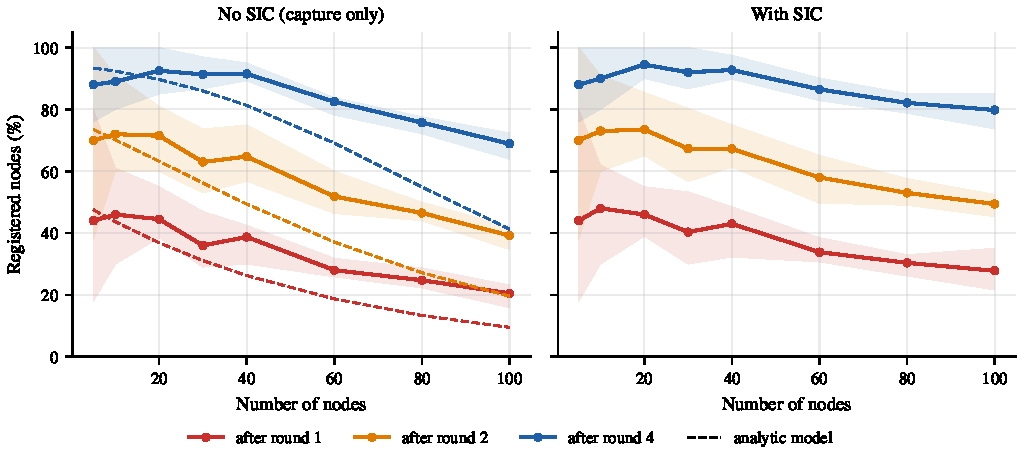
\includegraphics[width=\linewidth]{fig_registration}
\caption{Percentage of nodes registered after one, two and four discovery rounds against node count; mean over 10 runs with a $10$--$90\%$ band; left without SIC, right with SIC. Dashed: the mean-field model of Eq.~\eqref{eq:meanfield} with $p_a=\tfrac12$, $S=10$, $K=3$. This is \emph{our} re-creation of the paper's experiment (the paper's frame length and number of rounds are unknown), so only the qualitative trend is comparable.}
\label{fig:registration}
\end{figure}

Three observations from Figure~\ref{fig:registration}.
\begin{enumerate}
 \item \textbf{The trend reproduces the paper's.} Registration falls monotonically with density: after four rounds $\approx88\%$ at $5$ nodes, but only $69\%$ (no SIC) or $80\%$ (SIC) at $100$ nodes. More rounds recover more nodes (the paper does not say how many rounds it used).
 \item \textbf{At 5 nodes only $\approx44\%$ register in round one---not $\approx100\%$.} With five nodes collisions are rare, so something else limits participation. That something is $p_a\approx\tfrac12$: the base station advertises the slots of the \emph{current and the next} frame, and a node that picks one in the next frame is re-drawn by the next command and effectively sits the round out (Chapter~\ref{ch:bsengine}). The per-round gain then follows $1-0.5^k$: $50\%,75\%,87.5\%$; we measured $44\%,70\%,82\%,88\%$.
 \item \textbf{The model is a lower bound that tracks the shape.} It agrees at low density ($47.5\%$ against $44\%$ at $n=5$, round~1), then falls below the simulation at high density ($9.5\%$ against $21$--$28\%$ at $n=100$, round~1) because it ignores capture, SIC and the $5$~ms rule.
\end{enumerate}

\begin{reality}[Why even five nodes may not all register in one frame]
Observation~2 is not a radio effect at all. It is a consequence of the engine's two-frame RX look-ahead combined with a uniform random choice over the advertised slots. A protocol designer who tunes $S$ by Eq.~\eqref{eq:psucc} will find that the effective number of slots seen by a node is \emph{the advertised list}, i.e.\ twice the frame size, of which only half lie in the current frame. We discuss this in detail in Chapter~\ref{ch:bsengine}.
\end{reality}

\section{Design principles for energy-aware protocols}
\label{sec:principles2}

Putting the pieces together suggests a short checklist, each item testable in Amber.
\begin{enumerate}
 \item \textbf{Don't waste transmissions.} Prefer polls (no collisions) once nodes are known; during discovery, use frames somewhat larger than the expected number of contenders (Section~\ref{sec:energytwist}).
 \item \textbf{Exploit frequency orthogonality.} Assign shifts to spread nodes; collisions then occur only within a group.
 \item \textbf{Use the capture/SIC gain.} Near--far diversity is free; do not assume a collision is a loss.
 \item \textbf{Respect duty cycles.} A node is reachable only for a fraction $D=P_{\mathrm{in}}/P_{\mathrm{act}}$ of the time (Eq.~\eqref{eq:duty}); schedule redundancy accordingly.
 \item \textbf{Adapt.} Estimate the active population from observed outcomes (the custom demo's loop) and resize frames.
\end{enumerate}

\section{Chapter summary}
\begin{itemize}
 \item Ambient IoT protocols are reader-driven; Amber's default one has three commands (\code{send_id}, \code{ack}, \code{send_data}) and three node states (idle, wait\_ack, registered).
 \item Broadcast polling is cheap in commands but collides; unicast polling never collides but costs $N$ commands. The shipped unicast demo answers only $\approx9\%$ of polls: it is energy-limited.
 \item The base station cannot observe node energy states; silent nodes are ambiguous.
 \item A mean-field FSA model gives a lower bound on registration; our re-creation of the paper's experiment reproduces its downward trend.
 \item Engine behaviour (two-frame look-ahead) halves per-round participation: $\approx44\%$ registered after one round even at five nodes.
\end{itemize}

\begin{codemap}
\small
\begin{tabularx}{\linewidth}{@{}>{\ttfamily}p{5.2cm}X@{}}
\toprule
\normalfont\bfseries Concept & \normalfont\bfseries Code\\
\midrule
Command handling & \codew{BackscatterModule.handle_command}\\
Node protocol states & \codew{BackscatterModule.state}: \code{idle}, \code{wait_ack}, \code{registered}\\
ACK delivery & \codew{BSBehavior._send_pending_acks}\\
Pending / registered lists & \codew{nodes_pending_ack}, \codew{nodes_registered}\\
Broadcast vs unicast & \code{target} field: $-1$, int, or list\\
\bottomrule
\end{tabularx}
\end{codemap}

\section*{Exercises}
\begin{exercise}
Using Eq.~\eqref{eq:meanfield} with $p_a=1$, $S=10$, $K=3$ and $n_1=50$, compute the expected registered fraction after one round. Repeat with $p_a=\tfrac12$. By how many rounds does the latter lag?
\end{exercise}
\begin{exercise}
A unicast round for $N$ nodes takes $N(T_{\mathrm{cmd}}+T_{\mathrm{slot}})$. For $T_{\mathrm{cmd}}=5$~ms, $T_{\mathrm{slot}}=10$~ms and $N=100$, how long is a round? If each node can transmit at most once every $2$~s on average, what fraction of polls will be answered?
\end{exercise}
\begin{exercise}
Argue why unicast polling may nonetheless be preferable to broadcast even though it needs $N$ commands. Consider energy per delivered packet (Section~\ref{sec:energytwist}).
\end{exercise}
\begin{exercise}
List three observable quantities from which a base station could infer that a silent node is asleep rather than out of range, and say what each would cost the node.
\end{exercise}

\part{Simulation Methodology and Architecture}

\chapter{Discrete-Event Simulation and SimPy}
\label{ch:des}

\begin{defbox}[In this chapter you will learn]
\begin{itemize}
 \item what a simulation model is, and the difference between time-stepped and event-driven simulation;
 \item the SimPy concepts Amber uses: processes as generators, timeouts, and \emph{interrupts} as message passing;
 \item the rule that decides the order of events at the same instant, verified by experiment;
 \item why Amber pre-computes the radio channel, the measured cost per node and millisecond, and what limits scalability;
 \item how to think about randomness, replication, verification and validation.
\end{itemize}
\end{defbox}

\section{Models, state and time}
\label{sec:desmodel}

A simulation is an \emph{executable abstraction}. Its anatomy is always the same: a set of \emph{state variables} (a
capacitor voltage, a node's protocol state, a buffer of packets), a notion of \emph{time}, and \emph{rules} that change the state as time advances. The central design question is how time advances.

\paragraph{Time-stepped simulation.}
Advance the clock by a fixed $\Delta t$; at each step update every entity. This is simple and natural for
continuous dynamics such as a capacitor ($C\,\dot V=\dots$ integrated with step $\Delta t$). Its cost is proportional to
(simulated time)/$\Delta t$ whether or not anything happens.

\paragraph{Event-driven (discrete-event) simulation.}
Keep a \emph{future-event list} ordered by time. Repeatedly remove the earliest event, set the clock to its time, execute
it (which may schedule new events) and continue \citep{banks2010,law2015}. Nothing is computed between events, so a mostly idle system is cheap and an event's time can be arbitrary (not on a grid).

\begin{center}
\small
\renewcommand{\arraystretch}{1.15}
\begin{tabularx}{\linewidth}{@{}>{\sffamily\bfseries}p{3.0cm}XX@{}}
\toprule
 & Time-stepped & Event-driven\\
\midrule
Clock advances by & fixed $\Delta t$ & time of the next event\\
Natural for & continuous dynamics & sparse, asynchronous activity\\
Cost & $\propto T/\Delta t$ & $\propto$ number of events\\
Ordering at ties & implicit (loop order) & explicit rules\\
\bottomrule
\end{tabularx}
\end{center}

\begin{keyidea}[Amber is a hybrid]
The \emph{base station} is event-driven: it sleeps until a slot ends or a node interrupts it. The \emph{node} is
time-stepped: every node's controller schedules an event exactly $\SI{1}{ms}$ ahead, forever, because the capacitor must be integrated at a fixed step and thresholds must be checked
continuously. Consequently one controller wake-up per node per millisecond is the \emph{floor} of the simulator's cost: idle milliseconds cannot be skipped.
\end{keyidea}

\section{SimPy in ten minutes}
\label{sec:simpy}

Amber is built on SimPy \citep{simpy}, a process-based discrete-event framework for Python. Its ideas fit on one page.
\begin{itemize}
 \item An \code{Environment} holds the clock (\code{env.now}) and the future-event list.
 \item A \emph{process} is a Python \emph{generator function}. It runs until it hits a \code{yield}, which hands an \emph{event} to the scheduler; the process is
   suspended until that event occurs.
 \item \codew{yield env.timeout(d)} means ``wake me up $d$ time units from now''. Amber's time unit is the millisecond.
 \item \codew{env.process(gen)} starts a process; \codew{env.run(until=T)} runs the clock to $T$.
 \item \codew{proc.interrupt(cause)} \emph{throws} a \codew{simpy.Interrupt} exception into the target process at its current \code{yield}. The target can catch it, read \code{cause} (any object, in Amber a string), and carry on. This is how processes send each other messages.
\end{itemize}
A complete toy example: a charger adds one unit per millisecond; a supervisor interrupts it after $5$~ms.
\begin{lstlisting}
import simpy

def charger(env, cap):
    while True:
        try:
            yield env.timeout(1)          # wait 1 ms
            cap["q"] += 1                 # then add charge
        except simpy.Interrupt as it:     # a message arrives
            print(f"t={env.now}: charger interrupted ({it.cause})")
            return

def supervisor(env, proc):
    yield env.timeout(5)
    proc.interrupt("enough")              # send a message

env = simpy.Environment(); cap = {"q": 0}
p = env.process(charger(env, cap))
env.process(supervisor(env, p))
env.run(until=20)
print("final charge:", cap["q"])
\end{lstlisting}
Running it prints
\begin{verbatim}
t=5: charger interrupted (enough)
final charge: 4
\end{verbatim}
Notice that the charge is $4$, not $5$. At $t=5$ both the charger's own timeout and the supervisor's wake-up are due, yet the interrupt \emph{pre-empts}
the charger's increment. This is not an accident, as we show next.

\subsection{Order of events at the same instant}
\label{sec:tiebreak}

SimPy keeps events ordered by (time, priority, insertion counter). Ordinary events have priority \code{NORMAL} ($1$); \emph{interrupts are scheduled with priority
\code{URGENT} ($0$)}. We verified experimentally that an interrupt issued at time $t$ is handled \emph{at time $t$}, immediately after the issuing process yields and
before any other ordinary event at $t$. Three consequences are central to Amber:
\begin{enumerate}
 \item When the controller interrupts the capacitor, the capacitor's voltage update happens \emph{within the same millisecond}, before anything else at that instant; the controller's next
   reading (one millisecond later) sees the updated value.
 \item When a node's \code{do_transmit} interrupts the base station, the base station buffers that packet \emph{before} any other node's controller runs. The base station's ``scratch'' attributes
   (\codew{received_tag_id}, \codew{data_from_tag}, \dots) therefore act as a safe one-element mailbox, even if two nodes transmit in the same millisecond.
 \item Among \emph{ordinary} events at one instant the order is the order of scheduling, which is the order in which processes were created. Results can in principle depend on that order; Amber's controllers all wake at the same instants, so the order in which nodes are created is the order in which they run.
\end{enumerate}

\section{How Amber uses SimPy}
\label{sec:amberusessimpy}

Three kinds of process run concurrently.
\begin{center}
\small
\renewcommand{\arraystretch}{1.15}
\begin{tabularx}{\linewidth}{@{}>{\ttfamily}p{2.8cm}>{\raggedright}p{3.4cm}>{\raggedright\arraybackslash}X@{}}
\toprule
\normalfont\bfseries Process & \normalfont\bfseries Wakes on & \normalfont\bfseries Does\\
\midrule
Controller & timeout of $\SI{1}{ms}$, always & recompute harvest power; apply thresholds; advance the node FSM; interrupt its capacitor\\
Capacitor & interrupt from its controller (idle timeout of $\SI{10}{ms}$ otherwise) & apply one $\Delta t$ step selected by the interrupt's cause\\
BSBehavior & timeout at the end of each TX/RX slot; interrupt \codew{"receive_data"} from nodes & run the schedule; buffer packets during RX; resolve collisions at the end of the window\\
EnvEnergySource & timeout of $\SI{1}{ms}$ & move to the next row of the solar trace\\
\bottomrule
\end{tabularx}
\end{center}
Inter-process communication uses two idioms: \textbf{interrupts with a string cause} as a signal (\codew{"capacitor_charging"}, \codew{"receive_data"}), and \textbf{shared attributes} as the payload
(\codew{capacitor.current}, \codew{capacitor.voltage_source}, \code{bs.rssi_dbm}). The base station additionally calls node methods \emph{directly} (\codew{receive_command}); that call is synchronous and instantaneous.

\section{Precomputation and scalability}
\label{sec:scalability}

The paper states that ``since nodes and base stations are stationary, coverage maps and link budgets are pre-computed once before execution to minimize runtime overhead.'' With static geometry the downlink power $P_{\mathrm{dl}}$ of every node and the uplink
power to every sector are constants. Computing them once costs $O(N\cdot B\cdot S_B)$ (nodes $\times$ base stations $\times$ sectors) and is vectorised with NumPy. In our measurement the pre-computation for $300$ nodes took $\SI{3.4}{ms}$.

What remains at run time is the per-millisecond controller step. We measured the wall-clock cost of Amber with a fixed number of nodes over $\SI{5}{s}$ of simulated time (hybrid nodes, idle base station) on a $4$-core cloud container:

\begin{center}
\small
\renewcommand{\arraystretch}{1.1}
\begin{tabular}{@{}rrrr@{}}
\toprule
Nodes & Pre-computation & Run time ($5$ s sim.) & $\si{\micro s}$ per node-ms\\
\midrule
 10 & \SI{0.9}{ms} & \SI{0.57}{s} & 11.5\\
 30 & \SI{0.8}{ms} & \SI{1.87}{s} & 12.5\\
100 & \SI{1.4}{ms} & \SI{6.29}{s} & 12.6\\
300 & \SI{3.4}{ms} & \SI{21.3}{s} & 14.2\\
\bottomrule
\end{tabular}
\end{center}
The cost is \emph{linear} in the number of nodes at about $\SIrange{12}{14}{\micro s}$ per node-millisecond, so a $60$~s run with $1000$ nodes takes roughly $1000\times60\,000\times13\,\si{\micro s}\approx13$~minutes. This supports the paper's claim of ``efficient simulation of hundreds of nodes''
(about four times slower than real time for $300$ nodes in our measurement; your machine will differ).

\begin{reality}[Memory grows with time unless you ask it not to]
Every capacitor appends a \codew{(time, voltage)} tuple to \codew{voltage_history} \emph{every millisecond} while \codew{keep_logs=True} (the default), and the base station and backscatter modules store every packet. For long runs pass \codew{keep_logs=False}
(controller, capacitor, backscatter, base station) and use the base station's \code{stream_log} option, which writes packets to disk as they arrive; counters (\code{total_rx}, \codew{total_collided}, \dots) are always maintained at constant memory.
\end{reality}

\section{Randomness and replication}
\label{sec:random}

Several mechanisms in Amber are random: the start-up delay of each controller ($0$--$\SI{2}{s}$, uniform), the sensed value, the slot chosen by a node, and node placement in experiments. They all use Python's global \code{random} module,
\emph{unseeded by default}. Only the custom-protocol demo calls \code{random.seed}. Therefore two runs of, say, the broadcast demo differ slightly (we measured $122$ and $121$ packets sent in two runs; over ten seeds the mean is $124.4$ with standard deviation $1.6$).
Good practice, followed by the paper's experiment:
\begin{itemize}
 \item treat a single run as one sample; \emph{replicate} ($10$ runs per density in the paper) and report distributions (box plots) or means with confidence intervals;
 \item \codew{random.seed(s)} for reproducibility of any one run;
 \item vary only one factor at a time when attributing an effect (our SIC ablation, Section~\ref{sec:sicexperiment}).
\end{itemize}

\section{Verification, validation and what Amber has had}
\label{sec:vv}

\begin{description}[leftmargin=0.4cm,font=\sffamily\bfseries]
 \item[Verification] asks \emph{``Did we build the model right?''} (code implements the intended equations). Throughout this book we verified Amber against closed-form results: the exact RC solution (agreement to $2\times10^{-4}$~V),
   hand-computed link budgets (exact to two decimals), SIC arithmetic, and ALOHA-based expectations for registration.
 \item[Validation] asks \emph{``Did we build the right model?''} (it represents reality well enough for its purpose), usually by comparison with measurements. The paper is a demo abstract and presents no hardware comparison; the radio models are standard (Friis, 3GPP UMa) but
   the harvester, capacitor and node loads are idealisations. Treat Amber's \emph{relative} comparisons (protocol A versus B under identical assumptions) as more trustworthy than its \emph{absolute} numbers.
\end{description}
\begin{keyidea}
A simulator is a \emph{microscope for mechanisms}, not a crystal ball. Use it to see \emph{why} a protocol behaves as it does (energy gating, collision structure, capture), then confirm key numbers experimentally.
\end{keyidea}

\section{Chapter summary}
\begin{itemize}
 \item Time-stepped simulation suits continuous dynamics; event-driven suits sparse events; Amber combines both: an event-driven base station and $\SI{1}{ms}$ time-stepped nodes.
 \item In SimPy a process is a generator, \code{timeout} suspends it and \codew{interrupt(cause)} sends it a message; interrupts are \emph{urgent}, so they are handled at the same instant before ordinary events.
 \item Static geometry lets Amber pre-compute all link budgets; run time is linear in the number of nodes at $\approx13\,\si{\micro s}$ per node-ms.
 \item Randomness is unseeded by default; replicate and report distributions.
 \item Amber is verified against analytic cases in this book but not validated against hardware in the paper.
\end{itemize}

\section*{Exercises}
\begin{exercise}
Modify the toy example so that the supervisor interrupts at $t=5.5$ (use floating-point time). What is the final charge, and why?
\end{exercise}
\begin{exercise}
Explain why an event-driven simulator cannot skip idle milliseconds in Amber, and how you would restructure the node model so that it could. What accuracy would you lose?
\end{exercise}
\begin{exercise}
Using $13\,\si{\micro s}$ per node-ms, estimate the run time for $500$ nodes over $\SI{120}{s}$. How many replications of a $100$-node, $\SI{20}{s}$ experiment fit in one hour?
\end{exercise}
\begin{exercise}
Two nodes transmit in the same millisecond. Describe, step by step, how SimPy's ordering rules ensure that the base station buffers \emph{both} packets rather than overwriting the first.
\end{exercise}
\begin{exercise}
Why would you not report a protocol's performance from a single unseeded run? Design a minimal replication plan for the node-density experiment of the paper.
\end{exercise}

\chapter{The Architecture of Amber}
\label{ch:architecture}

\begin{defbox}[In this chapter you will learn]
\begin{itemize}
 \item the runtime object graph of an Amber scenario and who calls whom;
 \item the ``interface contracts'' between modules (duck typing), and the extension points that let you swap a capacitor, a protocol or a policy;
 \item the data dictionaries that carry pre-computed channel state;
 \item the eight-step recipe that every demo follows to wire a scenario;
 \item what happens in a single simulated millisecond.
\end{itemize}
\end{defbox}

\section{Objects at run time}
\label{sec:objects}

Figure~\ref{fig:modulemap} showed the \emph{import} structure. A running scenario has a different shape: for every node a trio of cooperating objects, and shared channel state.

\begin{figure}[t]
\centering
\begin{tikzpicture}[x=1cm,y=1cm,>=Stealth]
 % shared
 \node[mod,minimum width=3.3cm] (cov) at (7.4,5.8) {\code{CoverageMap}\\\scriptsize pre-computes channel; updates harvest power};
 \node[ext,minimum width=2.6cm] (src) at (12.2,5.8) {\code{EnvEnergySource}\\\scriptsize \code{ext_power}};
 \node[ext,minimum width=3.4cm] (dl) at (2.4,5.8) {\code{downlink_results}\\\code{uplink_results} (dicts)};
 % per node
 \draw[rounded corners=4pt,agreen,fill=lightgreen] (3.4,-0.2) rectangle (11.4,4.2);
 \node[lab,anchor=north west] at (3.5,4.15) {\textbf{one per node}};
 \node[mod,minimum width=2.4cm] (node) at (4.8,3.0) {\code{Node}\\\scriptsize data record};
 \node[mod,minimum width=2.6cm] (ctl) at (7.6,3.0) {\code{Controller}\\\scriptsize FSM, $\Vhigh$/$\Vlow$};
 \node[mod,minimum width=2.4cm] (cap) at (10.2,3.0) {\code{Capacitor}};
 \node[mod,minimum width=3.4cm] (bsm) at (7.6,0.7) {\code{BackscatterModule}\\\scriptsize protocol};
 % base station
 \node[mod,minimum width=3.0cm,fill=lightorange,draw=aorange] (bsb) at (1.0,0.7) {\code{BSBehavior}\\\scriptsize schedule / policy};
 \node[ext] (bsd) at (1.0,-1.2) {\code{BaseStation}\\\scriptsize sectors};
 % arrows
 \draw[->] (dl) -- node[lab,left]{read} ++(0,-1.2) -| (bsm.north west);
 \draw[->] (cov) -- node[lab,above]{writes \codew{harvesting_power_dbm}} (node.north east |- cov.south);
 \draw[->,dashed] (src) -- node[lab,above]{} (cov);
 \draw[->] (ctl) -- node[lab,above]{\codew{interrupt(cause)}} (cap);
 \draw[->] (ctl) -- node[lab,right]{\codew{controller_tx_ready}} (bsm);
 \draw[->] (bsm.west) -- node[lab,above]{\codew{interrupt("receive_data")}} (bsb.east);
 \draw[->] (bsb.north) .. controls +(0,1.8) and +(-1.5,0) .. node[lab,above left,pos=0.55]{\codew{receive_command}} (bsm.north west);
 \draw[->] (bsb) -- (bsd);
 \draw[->] (node) -- (ctl);
\end{tikzpicture}
\caption{Runtime object graph. Solid arrows are calls or attribute reads; the arrows labelled \code{interrupt} are SimPy messages. The coverage map is shared by all nodes; the \code{Capacitor}, \code{Controller} and \code{BackscatterModule} are instantiated once per node; a \code{BSBehavior} exists per base station.}
\label{fig:objgraph}
\end{figure}

\paragraph{Who owns time?}
Each of \code{Controller}, \code{Capacitor}, \code{BSBehavior} and \codew{EnvEnergySource} registers one SimPy process in its constructor (\codew{self.action = env.process(self.run())}). The \code{Node}, \code{Sector}, \code{BaseStation} are plain \emph{data records} (Python dataclasses); the \code{CoverageMap} is a calculator, not a process. The \codew{BackscatterModule} has \emph{no process of its own}: it is passive logic that other processes call.

\section{Interface contracts}
\label{sec:contracts}

Amber uses \emph{duck typing}: modules interact through a handful of attributes and methods rather than formal base classes. Knowing the contracts is knowing how to replace a module.

\begin{center}
\footnotesize
\renewcommand{\arraystretch}{1.15}
\begin{tabularx}{\linewidth}{@{}>{\sffamily\bfseries}p{3.0cm}>{\raggedright}X>{\raggedright\arraybackslash}p{2.3cm}@{}}
\toprule
Consumer & Needs from\ldots & Provided by default\\
\midrule
Controller & \emph{capacitor}: \codew{action.interrupt(cause)} for causes \codew{capacitor_charging}, \codew{capacitor_full}, \codew{capacitor_charge_and_discharge}; writable \code{current} (A) and \codew{voltage_source} (V); readable \code{voltage}, \codew{internal_time} (s) & \code{Capacitor}\\
Controller & \emph{backscatter}: \code{state}; \codew{controller_tx_ready(data)} returning a dict or \code{None}; \codew{do_transmit(tx_info)} & \codew{BackscatterModule}\\
Controller & \emph{node}: \code{id}, writable \code{state}, \codew{harvesting_power_dbm} (set by the coverage map) & \code{Node}\\
BackscatterModule & \emph{base-station process}: attributes \codew{received_tag_id}, \codew{data_from_tag}, \codew{rssi_dbm}, \codew{best_sector_idx}, \codew{subcarrier_shift}, and \codew{action.interrupt("receive_data")} & \code{BSBehavior}\\
BSBehavior & \emph{modules}: \codew{node.id}, \codew{receive_command(cmd,bs_id,data)} & \codew{BackscatterModule}\\
CoverageMap & \emph{nodes}: \code{id}, \code{x}, \code{y}, \code{height}, \code{efficiency}, \code{antenna_*}, \code{state}; \emph{base stations}: \code{id}, \code{x}, \code{y}, \code{sectors} & dataclasses\\
\bottomrule
\end{tabularx}
\end{center}

\paragraph{Extension points.} Three seams are designed for user code:
\begin{enumerate}
 \item \textbf{Node protocol:} subclass \codew{BackscatterModule} and override \codew{handle_command} (what to do on a command) and \codew{build_tx_payload} (what to send in your slot). Everything else---the sensitivity gate, logging, slot validation, uplink delivery---stays.
 \item \textbf{Base-station behaviour:} either give \code{BSBehavior} a static \code{schedule} list, or a \code{policy} generator that yields one frame at a time and can adapt to \codew{decoded_this_frame}, \codew{total_collided}, etc.
 \item \textbf{Energy models:} supply any object with the capacitor contract, a different \codew{node_ext_power_fn}, or another trace to \codew{EnvEnergySource}.
\end{enumerate}
Chapter~\ref{ch:extending} demonstrates (1) and (2) with the adaptive-ALOHA demo.

\section{Data dictionaries}
\label{sec:dicts}

Channel state is passed around as plain dictionaries produced once by the \code{CoverageMap}.

\paragraph{Downlink results} (\codew{compute_bs_to_point(nodes)}), keyed by node id:
\begin{center}
\small
\begin{tabularx}{\linewidth}{@{}>{\ttfamily}p{3.5cm}X@{}}
\toprule
\normalfont\bfseries Key & \normalfont\bfseries Content\\
\midrule
owner & name of the best serving sector, e.g.\ \code{"BS0_S0"}\\
best\_pw\_dbm, best\_pw\_w & strongest received power over all base stations and sectors\\
total\_pw\_dbm & power summed over all sectors (interference-like measure)\\
per\_node\_powers & $\{\text{node id}:\{\text{sector name}:\text{dBm}\}\}$, every sector\\
\bottomrule
\end{tabularx}
\end{center}

\paragraph{Uplink results} (\codew{compute_point_to_bs(nodes)}), keyed by sector name:
\codew{per_sector_powers[sector][node_id]} (dBm; the power that sector would receive from that node), plus per-sector \code{owner} (the strongest node), \code{best_pw_dbm}, \code{best_pw_w}, \codew{total_pw_dbm}.

\paragraph{Per-node attributes written by the coverage map}: \codew{harvesting_power_dbm} and \codew{backscatter_power_dbm}. These are \emph{not} fields of the \code{Node} dataclass; they are attached dynamically, so a controller will fail at its first step with an \codew{AttributeError} unless \codew{calculate_node_power} has been called for its node beforehand (as every demo does at set-up).

\section{The wiring recipe}
\label{sec:recipe}

All four demos, and the paper's experiment, follow the same eight steps. Learn them once.

\begin{enumerate}[label=\textbf{Step \arabic*.},leftmargin=1.6cm]
 \item \textbf{Define the topology.} Create \code{Node}s (position, height, antenna, sensitivity, efficiency, subcarrier shift) and \code{BaseStation}s with \code{Sector}s (azimuth, beamwidth, power, gain, sensitivity).
 \item \textbf{Create the environment and energy source.} \codew{env = simpy.Environment()}; optionally an \codew{EnvEnergySource} reading the solar trace with \codew{resistance=R_SERIES}.
 \item \textbf{Build one \code{CoverageMap} per energy mode.} \codew{node_energy_mode} is per map, so WPT-only and hybrid nodes use different maps (the demos do so).
 \item \textbf{Pre-compute the channel.} \codew{dl = cov.compute_bs_to_point(nodes)}; \codew{cov.calculate_node_power(nodes, dl)}; \codew{ul = cov.compute_point_to_bs(nodes)}. (Order matters: the uplink needs the backscatter power that \codew{calculate_node_power} writes.)
 \item \textbf{Instantiate the per-node trio.} \codew{Capacitor(env, id, params, initial_voltage)}; \codew{BackscatterModule(env, node, bs_processes=[], uplink_results=ul, downlink_results=dl)}; \codew{Controller(env, capacitor_ctrl, node, backscatter, params, coverage_map=cov, downlink_results=dl)}.
 \item \textbf{Instantiate the base station behaviour.} \codew{BSBehavior(env, base_station, schedule=... or policy=..., backscatter_modules=[...], enable_sic=...)}.
 \item \textbf{Close the loop.} Set every module's \codew{bs_processes = [bs_behavior]} (the module needs the process to interrupt, the process needs the modules to command; neither exists when the other is built). For demos that skip discovery: \codew{bsm.state = "registered"} and \codew{bs.nodes_registered = [...]}.
 \item \textbf{Run and read counters.} \codew{env.run(until=T_ms)}; then use \codew{bs.rx_packets}, \codew{bsm.tx_records}, \code{bs.total_rx}, \codew{bs.total_collided}, \dots
\end{enumerate}
Forgetting Step~7 produces the quietest of failures: a node whose \codew{bs_processes} is empty ``transmits'' (it logs a TX record with \codew{delivered=False}) but no base station ever hears it.

\section{One simulated millisecond}
\label{sec:onems}

Figure~\ref{fig:objgraph} shows who talks to whom; this table shows the \emph{order} within a single millisecond for one node (Chapter~\ref{ch:controller} gives the details of each step).

\begin{center}
\small
\renewcommand{\arraystretch}{1.15}
\begin{tabularx}{\linewidth}{@{}rlX@{}}
\toprule
\# & Actor & Action\\
\midrule
1 & Controller wakes & publishes its state name on the node (\code{node.state})\\
2 & Controller & \codew{coverage_map.calculate_node_power([node], downlink_results)}: new $P_h$ (depends on \code{node.state} and the solar trace)\\
3 & Controller & $\Vs=\sqrt{P_h R_s}$ written to \codew{capacitor.voltage_source}\\
4 & Controller & reads $V$ (the value left by the \emph{previous} millisecond's update); applies the hysteresis rule; runs \codew{working_mode()}, one FSM step, which sets \codew{capacitor.current} and calls \codew{capacitor.action.interrupt(cause)}\\
5 & Controller & in state \emph{wait\_slot}: \codew{controller_tx_ready}; if ready, \code{do_transmit}, which sets the base station's scratch fields and interrupts it\\
6 & Controller & \codew{yield env.timeout(1)}: suspends\\
7 & Capacitor (urgent, same ms) & applies one $\Delta t$ step and appends to its history\\
8 & Base station (urgent, same ms) & if in an RX window, buffers the packet\\
\bottomrule
\end{tabularx}
\end{center}
Steps~7 and~8 are SimPy \emph{urgent} events: they run at the same simulated instant, but only after the controller has yielded, and in the order in which the interrupts were issued.
At the \emph{end} of each RX window the base station processes its buffer (Algorithm~\ref{alg:rxbuffer}); at the \emph{start} of each TX window it calls the target modules' \codew{receive_command}, a synchronous call.

\begin{codemap}
\small
\begin{tabularx}{\linewidth}{@{}>{\ttfamily}p{4.4cm}X@{}}
\toprule
\normalfont\bfseries Concept & \normalfont\bfseries Where\\
\midrule
Per-node trio & constructed in every demo's \codew{run_simulation()}\\
Node protocol seam & \codew{BackscatterModule.handle_command}, \codew{.build_tx_payload}\\
BS policy seam & \codew{BSBehavior(policy=...)}, \code{_run_policy}\\
Channel dictionaries & \codew{CoverageMap.compute_*}\\
Time-owning objects & \code{Controller}, \code{Capacitor}, \code{BSBehavior}, \codew{EnvEnergySource}\\
\bottomrule
\end{tabularx}
\end{codemap}

\section{Chapter summary}
\begin{itemize}
 \item Four classes own SimPy processes; \codew{BackscatterModule} and \code{CoverageMap} are passive helpers; \code{Node}, \code{Sector}, \code{BaseStation} are data.
 \item Modules interact by duck-typed contracts: a capacitor must accept three interrupt causes and expose \code{voltage}, \code{current}, \codew{voltage_source}; a protocol module must provide \code{state}, \codew{controller_tx_ready}, \code{do_transmit}.
 \item Channel state lives in two dictionaries computed once; harvest and backscatter power are per-node attributes attached by the coverage map.
 \item Every scenario follows the same eight wiring steps; the commonest mistake is not attaching \codew{bs_processes}.
\end{itemize}

\section*{Exercises}
\begin{exercise}
Sketch the sequence diagram (UML style) of a unicast poll between \code{BSBehavior}, \codew{BackscatterModule}, \code{Controller} and \code{BSBehavior}'s buffer, using the objects of Figure~\ref{fig:objgraph}.
\end{exercise}
\begin{exercise}
You want to replace the capacitor by a supercapacitor with an equivalent series resistance and a voltage-dependent leakage. Which attributes and interrupt causes must your class provide? What else would need to change?
\end{exercise}
\begin{exercise}
Why must the uplink computation follow \codew{calculate_node_power}? What would the base station receive if it were computed first?
\end{exercise}
\begin{exercise}
List the objects you would create for a scenario of two base stations of three sectors and $50$ nodes, and count the SimPy processes that exist.
\end{exercise}

\part{Inside the Simulator}

\chapter{Topology and the Coverage Engine}
\label{ch:coverage}

\begin{defbox}[In this chapter you will learn]
\begin{itemize}
 \item every parameter of \code{Node}, \code{Sector} and \code{BaseStation}, with its unit, default and role;
 \item what the coverage map computes, and which of its outputs the \emph{simulation} actually uses;
 \item the algorithms for downlink, harvest/backscatter bookkeeping and uplink, step by step;
 \item how multiple base stations interact (and where the model simplifies);
 \item numerical conventions: sentinels, floors and the meaning of ``owner''.
\end{itemize}
\end{defbox}

\section{The topology objects}
\label{sec:topo}

Three small dataclasses in \file{radiodevices.py} describe the geometry and radio hardware. Coordinates are in metres on a flat plane ($x$ east, $y$ north); heights are separate.

\subsection{\texorpdfstring{\code{Node}}{Node}}

\begin{center}
\footnotesize
\renewcommand{\arraystretch}{1.12}
\begin{tabularx}{\linewidth}{@{}>{\ttfamily}p{3.4cm}>{\ttfamily}p{2.1cm}>{\raggedright}p{2.5cm}>{\raggedright\arraybackslash}X@{}}
\toprule
\normalfont\bfseries Field & \normalfont\bfseries Default & \normalfont\bfseries Unit & \normalfont\bfseries Role\\
\midrule
id & required & -- & identifier used in all dictionaries and logs\\
x, y & required & m & position\\
height & 1.5 & m & $h_{UT}$ in UMa path loss\\
antenna\_type & "omni" & -- & \texttt{"omni"} or \texttt{"3GPP"}\\
antenna\_gain\_dbi & 0.0 & dBi & peak gain (omni: constant)\\
azimuth\_deg, beamwidth\_deg & 0, 360 & deg (compass) & only for 3GPP node antennas\\
efficiency & 1.0 & ratio & $\eta$: fraction of received power reflected\\
sensitivity\_dbm & $-45$ & dBm & weakest downlink command the node notices\\
subcarrier\_shift & 0 & integer & frequency-domain group for uplink\\
node\_type & "passive" & -- & cosmetic (plot colour)\\
radius, color, label & 2, "", True & plot & drawing only\\
state & "listening" & -- & written by the \code{Controller} each ms; \emph{not} a constructor argument\\
\bottomrule
\end{tabularx}
\end{center}

\subsection{\texorpdfstring{\code{Sector}}{Sector} and \texorpdfstring{\code{BaseStation}}{BaseStation}}

\begin{center}
\footnotesize
\renewcommand{\arraystretch}{1.12}
\begin{tabularx}{\linewidth}{@{}>{\ttfamily}p{3.4cm}>{\ttfamily}p{2.1cm}>{\raggedright}p{2.5cm}>{\raggedright\arraybackslash}X@{}}
\toprule
\normalfont\bfseries Field & \normalfont\bfseries Default & \normalfont\bfseries Unit & \normalfont\bfseries Role\\
\midrule
\multicolumn{4}{@{}l}{\textbf{Sector}}\\
azimuth\_deg & required & deg (compass) & boresight\\
beamwidth\_deg & required & deg & $\varphi_{3\mathrm{dB}}$ of the 3GPP pattern\\
power & 43.0 & dBm & transmit power (the paper uses 30)\\
antenna\_gain\_dbi & 17.0 & dBi & $G_{\max}$\\
antenna\_type & "3GPP" & -- & or \texttt{"omni"} (0 dBi, ignores gain field)\\
height & 25.0 & m & $h_{BS}$\\
sensitivity\_dbm & $-100$ & dBm & weakest backscatter packet logged\\
\midrule
\multicolumn{4}{@{}l}{\textbf{BaseStation}}\\
id, x, y & required & m & identity and position of the mast\\
sectors & [] & list & any number of sectors\\
\bottomrule
\end{tabularx}
\end{center}

\paragraph{A subtle asymmetry.} An \texttt{"omni"} \emph{node} uses its \codew{antenna_gain_dbi}; an \texttt{"omni"} \emph{sector} is forced to $\SI{0}{dBi}$ (\codew{antenna_from_sector} ignores the gain field). Use \texttt{"3GPP"} with a wide beamwidth if you want a high-gain wide beam.

\section{The CoverageMap}
\label{sec:covmap}

\code{CoverageMap} is a configuration object plus four calculators.

\begin{center}
\small
\renewcommand{\arraystretch}{1.12}
\begin{tabularx}{\linewidth}{@{}>{\ttfamily}p{3.7cm}>{\ttfamily}p{2.1cm}X@{}}
\toprule
\normalfont\bfseries Parameter & \normalfont\bfseries Default & \normalfont\bfseries Meaning\\
\midrule
base\_stations, nodes & \texttt{None} & the topology\\
freq\_hz & 925e6 & carrier (demos: 924e6)\\
pathloss\_model & "macro" & \texttt{"fspl"} or \texttt{"macro"}\\
los & True & LOS or NLOS branch of UMa\\
extra\_np\_per\_m & 0 & medium attenuation (power, Np/m)\\
node\_energy\_mode & "wpt" & \texttt{"wpt"}, \texttt{"external"}, \texttt{"hybrid"}\\
node\_ext\_power\_fn & \texttt{None} & callback $\text{node}\to$ watts\\
combine\_mode & "max" & hybrid: \texttt{"max"} or sum\\
bandwidth\_hz, noise\_figure\_db & 100e6, 6 & \emph{declared ``for SNR'' but never used in this class}\\
\bottomrule
\end{tabularx}
\end{center}

\subsection{The coverage grid (for pictures)}

\codew{compute_coverage_map(xmin,xmax,ymin,ymax,step)} evaluates, on a regular grid, the received power from every sector of every base station (receiver antenna $\SI{0}{dBi}$, receiver height $\SI{1.5}{m}$) and stores the \emph{maximum} over sectors (\code{best_pw_dbm}), the \emph{sum} (\codew{total_pw_dbm}) and the name of the best sector (\code{owner}). \code{plot_rssi} draws it. The paper's Figure~1 is this picture. Crucially, \textbf{the simulation does not use the grid}; it is a diagnostic, which is why the demos' coverage maps are computed but never read at run time.

\subsection{Downlink to the nodes}

\codew{compute_bs_to_point(nodes)} is the workhorse. For each base station, sector and node:
\begin{enumerate}
 \item horizontal distance $d_{2D}$ from the mast to the node;
 \item bearing from the mast to the node, angular error to the sector's boresight, sector gain $G_s(\varphi)$ (Chapter~\ref{ch:antennas});
 \item bearing from the node back to the mast, angular error to the node's own boresight, node gain $G_n(\varphi')$;
 \item received power $P=P_{\mathrm{tx}}\,G_s\,L(d)\,e^{-\alpha d}\,G_n$ with $h_{BS}$ from the sector and $h_{UT}$ from the node (Chapter~\ref{ch:pathloss});
 \item bookkeeping: store each sector's power in \codew{per_node_powers}; keep the running maximum (\code{best_pw_w}, with the winning sector name as \code{owner}) and the sum (\codew{total_pw_dbm}).
\end{enumerate}
The calculation is vectorised over nodes with NumPy and looped over sectors.

\begin{keyidea}[``Best'' means maximum, not sum]
The power a node harvests is the \emph{strongest single sector's} power, not the sum of all carriers reaching it. Real carriers from several sectors at the same frequency would add (incoherently); Amber ignores them. This is conservative for energy but also means \emph{there is no inter-cell interference in the downlink}.
\end{keyidea}

\subsection{Harvest and backscatter power}

\codew{calculate_node_power(nodes, downlink_results)} converts the best downlink power into each node's \codew{harvesting_power_dbm} and \codew{backscatter_power_dbm} following the table of Section~\ref{sec:amberharvest} (three energy modes). It is called \emph{once} during set-up, and thereafter by each node's controller \emph{every millisecond} with $\text{nodes}=[\text{itself}]$, because the harvest depends on the node's state name and on the solar trace.

\subsection{Uplink to the base stations}

\codew{compute_point_to_bs(nodes)} takes each node's \codew{backscatter_power_dbm} (\textbf{evaluated at set-up, with the node in its initial state}) as a transmit power and propagates it to every sector: node gain toward the mast, path loss, sector receive gain. The result \codew{per_sector_powers[sector][node]} is the RSSI that sector would observe. The aggregates (\code{owner}, \code{best_pw_dbm}, \codew{total_pw_dbm}) are per sector.

\subsection{What this means for multiple base stations}

Three consequences of the dictionaries' design:
\begin{enumerate}
 \item \textbf{Every base station can hear every node.} \codew{per_sector_powers} contains an entry for each (sector, node) pair; no entry is dropped for being weak. When a node transmits, \code{do_transmit} interrupts \emph{each} base station in its \codew{bs_processes}, using the strongest sector of that base station. Whether a packet is \emph{logged} is decided afterwards by each sector's sensitivity. A cell-edge node is thus heard by several base stations at once (macro-diversity), and the paper's \codew{nodes_multi_bs} statistic counts exactly this.
 \item \textbf{Command reception ignores which base station spoke.} A node accepts a command if its \emph{best} downlink power over \emph{all} base stations exceeds its sensitivity, whichever base station issued the command.
 \item \textbf{Static link budgets.} Nothing changes with time except the harvest; in particular the uplink RSSI is a constant for each (sector, node) pair.
\end{enumerate}

\section{Numerical conventions}
\label{sec:numconv}

\begin{itemize}
 \item \textbf{Floor at $\SI{-120}{dBm}$}: \codew{watts_to_dbm} clamps at $10^{-15}$~W; a node with zero harvest has $\SI{-120}{dBm}$ and \codew{dbm_to_watts} returns $10^{-15}$, not zero.
 \item \textbf{Sentinel $\SI{-999}{dBm}$}: used when a node has no recorded power (e.g.\ \codew{received_power = best_pw_dbm.get(id, -999.0)}); it ensures commands are rejected and uplinks vanish rather than crash.
 \item \textbf{Tie-breaking}: the best sector is chosen by a strict ``$>$'', so ties go to the earlier-evaluated sector (first base station, lowest sector index).
 \item \textbf{Sector names} are strings \codew{BS<id>_S<index>}. The node module finds a base station's sectors by prefix matching on \code{BS<id>_} and recovers the sector index by splitting on \code{_S}; use integer base-station ids and let sectors be numbered by list order.
\end{itemize}

\begin{reality}[Where the coverage engine differs from physics]
(i) No inter-cell interference or carrier summation (``max'' not ``sum''); (ii) the uplink assumes the node reflects its \emph{initial-state} backscatter power at all times; (iii) the path loss near the mast has the artefacts of Chapter~\ref{ch:pathloss}; (iv) \codew{bandwidth_hz} and \codew{noise_figure_db} on the map are not used (noise is computed in the base station from its own arguments, Chapter~\ref{ch:bsengine}); (v) static geometry and no shadowing.
\end{reality}

\begin{codemap}
\small
\begin{tabularx}{\linewidth}{@{}>{\ttfamily}p{5.0cm}X@{}}
\toprule
\normalfont\bfseries Concept & \normalfont\bfseries Function (\file{propagation.py})\\
\midrule
Grid for pictures & \codew{compute_coverage_map}, \code{plot_rssi}\\
Downlink to nodes & \codew{compute_bs_to_point}\\
Harvest/backscatter & \codew{calculate_node_power}\\
Uplink to sectors & \codew{compute_point_to_bs}\\
Device drawing & \codew{_draw_radio_devices}\\
\bottomrule
\end{tabularx}
\end{codemap}

\section{Chapter summary}
\begin{itemize}
 \item Three dataclasses describe the hardware; units are metres, degrees (compass), dBm and dBi.
 \item The coverage grid is for plotting; the simulation uses \codew{compute_bs_to_point}, \codew{calculate_node_power} and \codew{compute_point_to_bs}.
 \item A node harvests the \emph{best sector's} power; every base station hears every node, gated by sector sensitivity.
 \item The uplink is computed once and uses the node's initial-state backscatter power.
\end{itemize}

\section*{Exercises}
\begin{exercise}
For a node at $(60,80)$ and a base station at the origin with sectors at compass azimuths $0^\circ$ and $120^\circ$ ($65^\circ$, $G_{\max}=\SI{15}{dBi}$, $\SI{46}{dBm}$, $h_{BS}=\SI{25}{m}$), which sector is the owner? Give the angular errors and the downlink power with UMa LOS and a $\SI{0}{dBi}$ node.
\end{exercise}
\begin{exercise}
Why does \codew{compute_point_to_bs} not need the base station's transmit power? What does it need from a previous call?
\end{exercise}
\begin{exercise}
A node lies equidistant from two base stations with identical sectors and both can hear it. Describe, with reference to the data structures, what the node's transmission triggers in each base station.
\end{exercise}
\begin{exercise}
Modify the harvest model (conceptually) so that a node harvests the \emph{sum} of all sectors' powers. Which function changes, and what data does it already have?
\end{exercise}

\chapter{The Node Controller}
\label{ch:controller}

\begin{defbox}[In this chapter you will learn]
\begin{itemize}
 \item the controller's per-millisecond loop, as an algorithm;
 \item the five states of the working-mode state machine, what each costs in charge and energy, and how states are chained;
 \item the start-up behaviour and the activation/shut-down hysteresis, from the code's point of view;
 \item the \emph{wait\_slot} state and its idealisations;
 \item the ``delivered-before-paid'' behaviour, measured: nearly half of the transmit states in the demo end in brown-out.
\end{itemize}
\end{defbox}

The \code{Controller} is the heart of a node. It owns the node's simulated \emph{behaviour}: it turns the capacitor voltage into duty-cycled activity (Chapter~\ref{ch:capacitor}), and activity into energy consumption and radio transmissions. Every node has one; each is a SimPy process that wakes up every millisecond.

\section{Configuration}

\codew{ControllerParams} bundles three frozen dataclasses (plus a maximum start-up time):
\begin{center}
\small
\renewcommand{\arraystretch}{1.12}
\begin{tabular}{@{}lrrrr@{}}
\toprule
State & Duration $d$ (ms) & Current $I$ (mA) & Charge $d\,I$ ($\si{\micro C}$) & Energy at $\SI{1.5}{V}$ ($\si{\micro J}$)\\
\midrule
listening & 5 & 0.14 & 0.70 & 1.05\\
sensing & 2 & 0.512 & 1.02 & 1.54\\
processing & 5 & 1.28 & 6.40 & 9.60\\
transmitting & 15 & 5.0 & 75.0 & 112.5\\
\midrule
\textbf{cycle} & 27 & -- & 83.1 & 124.7\\
\bottomrule
\end{tabular}
\end{center}
(demo values; the last column assumes a constant $\SI{1.5}{V}$). Transmitting is $90\%$ of the energy of a cycle. Thresholds are $\Vhigh=1.7$, $\Vlow=1.3$ \si{V}. \codew{max_startup_time_ms} (default $2000$) bounds a random start-up delay.

\begin{reality}[These demo loads are far from microwatt tags]
A transmit current of $\SI{5}{mA}$ at $\SI{1.5}{V}$ is $\SI{7.5}{mW}$, and the cycle averages $\SI{4.6}{mW}$. These are the electrical currents of a microcontroller-and-radio sensor node, three to four orders of magnitude above the $\sim\SI{1}{\micro W}$ class that 3GPP's first Ambient IoT release targets (Chapter~\ref{ch:intro}). They are parameters: nothing in the model prevents you from entering $\SI{1}{\micro A}$-class numbers, but the \emph{shipped demos} should not be read as representative of Ambient-IoT-class power.
\end{reality}

\section{The main loop}
\label{sec:ctlloop}

Algorithm~\ref{alg:ctlloop} is the \codew{Controller.run} generator in plain words.

\begin{algorithm}[t]
\caption{Controller main loop (every millisecond)}
\label{alg:ctlloop}
\begin{algorithmic}[1]
\State \textbf{each ms:} \quad publish \code{node.state}$\gets$ \code{state_name}
\State recompute harvest: \codew{calculate_node_power([node], downlink_results)} \quad \Comment{only if a map and results exist}
\State $\Vs\gets\sqrt{P_h\cdot R_s}$, \quad write to \codew{capacitor.voltage_source}
\If{\codew{capacitor.internal_time} $\le$ \codew{startup_delay}}
   \State interrupt capacitor with \texttt{charging}
\Else
   \State $v\gets$ \codew{capacitor.voltage}
   \If{$v\ge\Vhigh$ \textbf{and not} active}
      \State interrupt \texttt{full} (leak only); state$\gets$ listening; counter$\gets0$; active$\gets$ true
   \ElsIf{not active}
      \State interrupt \texttt{charging}; state$\gets$ listening
   \ElsIf{$v>\Vlow$}
      \State \Call{WorkingMode}{} \Comment{one FSM step; sets load and interrupts}
   \Else \Comment{$v\le\Vlow$ and active}
      \State active$\gets$ false; record FSM cycles of this charge cycle; interrupt \texttt{charging}
   \EndIf
\EndIf
\State \textbf{wait} 1 ms
\end{algorithmic}
\end{algorithm}

A few observations from the algorithm.
\begin{itemize}
 \item The \textbf{start-up delay} (uniform in $[0,2000)$~ms, drawn once per node) is measured on the \emph{capacitor's} own clock. During it the node charges even if $V$ already exceeds $\Vhigh$. Its purpose is to de-synchronise nodes that would otherwise all become active at the same simulated instant.
 \item \textbf{Activation} requires $v\ge\Vhigh$ \emph{and} the delay to have elapsed. At that moment the controller sends one \emph{leak-only} step (\texttt{capacitor\_full}), resets its state machine to \emph{listening} and sets the node active.
 \item \textbf{Shut-down} happens at the first millisecond where $v\le\Vlow$, \emph{wherever the state machine happens to be}.
 \item The voltage that the controller reads at step $k$ is the one produced by the capacitor update of step $k-1$ (Section~\ref{sec:onems}); the one-millisecond lag is harmless.
 \item The harvest power is recomputed in \emph{every} step: it changes when the node enters the \emph{transmitting} state (the $(1-\eta)$ rule of Chapter~\ref{ch:backscatter}) and with the solar trace.
\end{itemize}

\begin{reality}[The series resistance is not read from the capacitor]
Line~3 converts power to voltage using \codew{getattr(capacitor_ctrl, "R_series", 5e3)}. But \code{Capacitor} stores its resistance inside \code{params} (\codew{capacitor.params.R_series}); it has no attribute \code{R_series}. The \code{getattr} therefore \emph{always returns the default $\SI{5}{k\ohm}$}, whatever \codew{CapacitorParams.R_series} says. We verified this with a capacitor configured for $\SI{1}{k\ohm}$: \codew{hasattr(cap,"R_series")} is false and the lookup returns $5000$. In the shipped demos both values are $\SI{5}{k\ohm}$, so nothing goes wrong; if you change $R_s$ in \codew{CapacitorParams} without also changing the constant in \codew{Controller.run}, the equivalent source voltage and the capacitor's charging resistance will silently disagree.
\end{reality}

\section{The working-mode state machine}
\label{sec:fsm}

Once the node is active and $V>\Vlow$, each millisecond runs one step of the finite-state machine in Figure~\ref{fig:fsm}.

\begin{figure}[t]
\centering
\begin{tikzpicture}[>=Stealth,scale=0.95,transform shape]
 \node[st,fill=ablue!15,draw=ablue,minimum width=2.6cm] (L) at (0,0) {listening\\5\,ms, 0.14\,mA};
 \node[st,fill=agreen!15,draw=agreen,minimum width=2.6cm] (S) at (4.4,0) {sensing\\2\,ms, 0.51\,mA};
 \node[st,fill=apurple!15,draw=apurple,minimum width=2.6cm] (P) at (8.8,0) {processing\\5\,ms, 1.28\,mA};
 \node[st,fill=agold!40,draw=agold!80!black,minimum width=2.6cm] (W) at (8.8,-2.7) {wait\_slot\\no load, charging};
 \node[st,fill=ared!12,draw=ared,minimum width=2.6cm] (T) at (4.4,-2.7) {transmitting\\15\,ms, 5\,mA};
 \draw[->] (L) -- node[lab,above]{registered} (S);
 \draw[->] (S) -- (P);
 \draw[->] (P) -- (W);
 \draw[->] (W) -- node[lab,above,align=center]{slot valid:\\\code{do_transmit}} (T);
 \draw[->] (T.west) -| node[lab,pos=0.2,above]{done} (L.south);
 \draw[->] (L.north) -- ++(0,0.9) -| (12.3,-2.7) -- (W.east);
 \node[lab] at (6.2,1.12) {not registered: skip sensing and processing};
 \node[lab,align=center] at (4.4,-4.1) {if $V\le\Vlow$ in \emph{any} state the node switches off};
\end{tikzpicture}
\caption{The working-mode FSM. Numbers are the demo durations and currents. A node that is not yet registered skips sensing and processing (upper loop) and waits for a command (\emph{send\_id}) to give it a slot. A freshly registered node that has no sensor value yet returns from \emph{wait\_slot} to \emph{sensing} first.}
\label{fig:fsm}
\end{figure}

\paragraph{Mechanics common to all states.} A state is advanced by a \emph{counter} that increases by one each millisecond; the state ends when the counter reaches its configured duration. In every state except \emph{wait\_slot} the controller sets \codew{capacitor.current} to the state's current and sends the \texttt{charge\_and\_discharge} interrupt: the node \emph{draws} its load while the harvester \emph{charges} simultaneously.

\begin{description}[leftmargin=0.4cm,font=\sffamily\bfseries]
 \item[listening] ($d=5$): the receive window in the model's vocabulary. At its end a \emph{registered} node moves to \emph{sensing}; an unregistered one to \emph{wait\_slot}, where it can send its ID if a slot was offered.
 \item[sensing] ($d=2$): produces a sensor value (a random integer in $[100,255]$ in the stub); then \emph{processing}.
 \item[processing] ($d=5$): copies the sensed value to \codew{processed_data}; then \emph{wait\_slot}.
 \item[wait\_slot]: \textbf{draws no load and only charges}. Each millisecond the controller asks the protocol module whether a transmission is permitted now (\codew{controller_tx_ready}). If so, it \emph{immediately} calls \code{do_transmit}, records the data and moves to \emph{transmitting}.
 \item[transmitting] ($d=15$): draws $\SI{5}{mA}$ for $\SI{15}{ms}$; at the end the cycle count is incremented and the node returns to \emph{listening}.
\end{description}
Because \emph{wait\_slot} has no end condition other than a transmission (or the voltage dropping to $\Vlow$, impossible while no load is drawn and the harvester is charging), a node with nothing to say simply \emph{rests at full charge} until the base station gives it a slot. This is why the node-0 voltage in Figure~\ref{fig:sawtooth} climbs above $\SI{1.7}{V}$ during waiting.

\begin{reality}[Idealisations of \emph{wait\_slot}]
(i) Waiting draws \emph{zero} current. A real node must keep its wake-up receiver or timer alive: even $\SI{1}{\micro A}$ is not nothing. (ii) The listening state's ``receive window'' has no effect on whether commands are received (Chapter~\ref{ch:bsmodule}): commands are accepted in any state, including when the node is off.
\end{reality}

\section{One real energy cycle}
\label{sec:realcycle}

Figure~\ref{fig:fsmzoom} zooms into two transmissions of Node~0 from the broadcast demo ($\approx\SI{120}{ms}$), with the base-station slot structure underneath.

\begin{figure}[t]
\centering
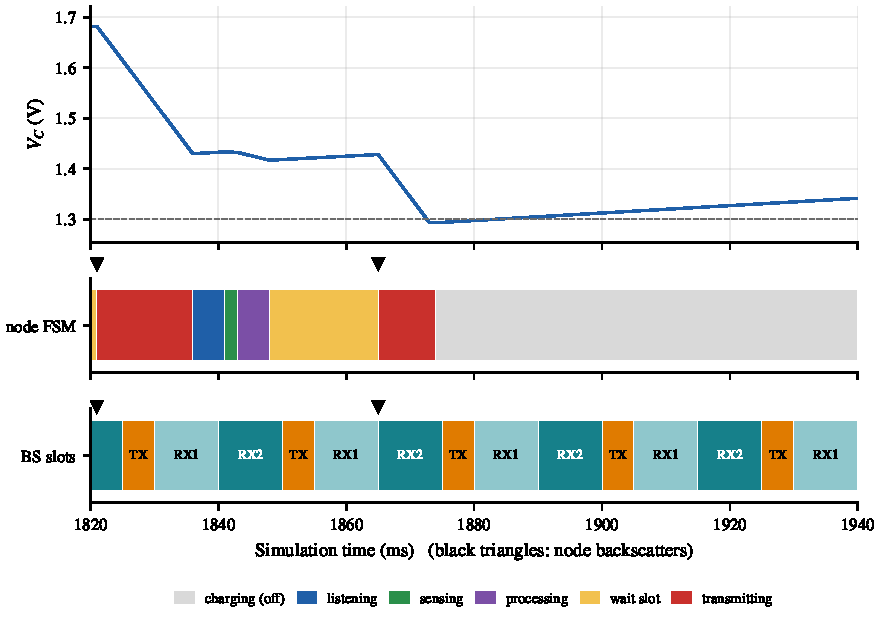
\includegraphics[width=\linewidth]{fig_fsm_zoom}
\caption{A $\SI{120}{ms}$ window of Node~0 (measured). Top: capacitor voltage; middle: the node's FSM state per millisecond (gold: waiting for a slot; grey: switched off and charging); bottom: the base station's frame (TX $\SI{5}{ms}$, two RX windows of $\SI{10}{ms}$). Black triangles mark the instants at which the node backscatters. Each packet is delivered at the \emph{start} of the node's transmit state, inside an RX window.}
\label{fig:fsmzoom}
\end{figure}

We can read off the entire mechanism.
\begin{enumerate}
 \item The first red bar is a full $\SI{15}{ms}$ transmit state: $V$ falls from $1.68$ to about $1.43$ V, i.e.\ $\Delta V=I\,T/C=\SI{0.25}{V}$ as predicted in Chapter~\ref{ch:capacitor}.
 \item Listening (blue), sensing (green) and processing (purple) follow, with a small drop each.
 \item During the gold \emph{wait\_slot} bar the voltage \emph{rises} (charge only). The wait ends at $\SI{1865}{ms}$, the first millisecond of the base station's next RX window in which the node holds a valid slot.
 \item The second transmit state starts, but $V$ reaches $\Vlow=\SI{1.3}{V}$ after only $9$~ms; the node \emph{switches off in the middle of its transmission}, and then charges (grey) for the next second.
\end{enumerate}

\begin{reality}[Delivered before paid]
The packet of the second transmission was handed to the base station at the first millisecond of the transmit state, \emph{before} the node paid the remaining $\SI{15}{ms}$ of energy. The controller's source says so explicitly: ``the \codew{transmitting} state \ldots\ only models the transmit energy draw; \ldots\ the reception has already happened.'' The consequence is energy \emph{causality}: nothing prevents a node from starting a transmission that its capacitor cannot finish, and it is still counted as delivered. We measured how often it happens in the shipped broadcast demo ($\SI{20}{s}$, one run): Node~0 had $25$ complete and $22$ truncated transmit states ($47\%$ truncated), Node~1 $9$ and $9$ ($50\%$), Node~2 $32$ and $24$ ($43\%$). Truncated states lasted only $9$--$\SI{11}{ms}$ instead of $\SI{15}{ms}$. A model in which a truncated burst counted as a \emph{lost} packet would report roughly half the throughput. This also explains the ``two packets per saw-tooth tooth'' of Chapter~\ref{ch:capacitor}. The design rule of that chapter applies: choose $C$, $\Vhigh$ and $\Vlow$ so that the energy window covers a full burst, or add a minimum-start voltage check before entering \emph{transmitting}.
\end{reality}

\section{Bookkeeping and logging}

\begin{itemize}
 \item \codew{fsm_count_in_current_cap_cycle} counts \emph{completed} FSM cycles (incremented at the end of \emph{transmitting}); on each shut-down it is appended to \codew{fsm_counts_per_cap_cycle}. In the demo these lists contain mostly $1$s, which is the footprint of the truncated second transmission above.
 \item \codew{data_history} records \codew{(capacitor time, value)} for every delivered datum of a registered node.
 \item \codew{acc_current_*} lists store the current of every step per state when \codew{keep_logs=True}.
 \item \codew{keep_logs=False} suppresses all per-step lists (flat memory for long runs).
\end{itemize}

\begin{codemap}
\small
\begin{tabularx}{\linewidth}{@{}>{\ttfamily}p{5.0cm}X@{}}
\toprule
\normalfont\bfseries Concept & \normalfont\bfseries Code (\file{controller.py})\\
\midrule
Currents, durations, thresholds & \codew{ControllerParams} (\code{CurrentsA}, \code{DurationsMs}, \codew{VoltageThresholdsV})\\
Main loop & \codew{Controller.run}\\
State machine & \codew{Controller.working_mode}\\
Charge-and-discharge request & \codew{Controller._enter_charge_and_discharge}\\
Registered? & \codew{Controller._is_registered}\\
Start-up delay & \codew{startup_delay_s}, from \codew{max_startup_time_ms}\\
\bottomrule
\end{tabularx}
\end{codemap}

\section{Chapter summary}
\begin{itemize}
 \item The controller wakes every ms, recomputes harvest, applies hysteresis and steps a five-state FSM; each active state draws its current while charging.
 \item A cycle costs $\approx83\,\si{\micro C}$, $\approx125\,\si{\micro J}$ at $\SI{1.5}{V}$, $90\%$ in the transmit state.
 \item \emph{wait\_slot} idles for free and charges; a node can rest above $\Vhigh$ indefinitely.
 \item Packets are delivered at the \emph{entry} of the transmit state; in the demo $43$--$50\%$ of transmit states are cut short by brown-out.
 \item The controller's conversion $\Vs=\sqrt{P_h R_s}$ always uses $R_s=\SI{5}{k\ohm}$, not the capacitor's parameter.
\end{itemize}

\section*{Exercises}
\begin{exercise}
Compute the energy of one FSM cycle at $\SI{1.7}{V}$ and at $\SI{1.3}{V}$ (charge is the same). By how much does the cycle's energy cost depend on the voltage at which it is run?
\end{exercise}
\begin{exercise}
A node is at $\SI{1.35}{V}$ when it enters \emph{transmitting}. Ignoring harvest and leakage, how long can it transmit before $\Vlow$? Express as a fraction of the $15$~ms burst. What minimum entry voltage guarantees a complete burst?
\end{exercise}
\begin{exercise}
Propose a one-line change to \code{wait_slot} that prevents transmissions from starting when the capacitor cannot complete them. What effect on throughput and on ``delivered'' statistics would you expect?
\end{exercise}
\begin{exercise}
Explain why the start-up delay is needed, and what the demo's collision statistics would look like for $N$ nodes if every node had a delay of zero and identical parameters.
\end{exercise}

\chapter{The Backscatter Module: Node-Side Protocol}
\label{ch:bsmodule}

\begin{defbox}[In this chapter you will learn]
\begin{itemize}
 \item the division of labour between \code{Controller} (energy and timing) and \codew{BackscatterModule} (protocol);
 \item the full path of a command: sensitivity gate, logging, slot bookkeeping, protocol handler;
 \item the four conditions a transmission must satisfy before it is allowed (\codew{controller_tx_ready}), and the exact slot-window arithmetic;
 \item what \code{do_transmit} computes and writes into the base station, and what the \code{delivered} flag \emph{really} means;
 \item how to override the protocol with two small methods.
\end{itemize}
\end{defbox}

\section{Division of labour}

The class docstring states it in one line: ``Controller handles energy/timing, BackscatterModule handles protocol.'' The module is \emph{passive}: it owns no SimPy process, only state and methods called by (i) the base station, to deliver commands, and (ii) the controller, to ask whether it may transmit and to perform the transmission.

\begin{center}
\small
\renewcommand{\arraystretch}{1.12}
\begin{tabularx}{\linewidth}{@{}>{\ttfamily}p{3.6cm}X@{}}
\toprule
\normalfont\bfseries Attribute & \normalfont\bfseries Meaning\\
\midrule
state & \texttt{"idle"}, \texttt{"wait\_ack"}, \texttt{"registered"}\\
rx\_slots & list of $(\text{start},\text{end})$ ms tuples advertised by the last command\\
chosen\_slot\_idx & index into \code{rx_slots} chosen by this node, or $-1$\\
\codew{last_tx_command_time} & time of the last command that enables a reply, or $-1$\\
tx\_records, rx\_records & logs of transmissions and received commands\\
packets\_sent, packets\_delivered, acks\_received & counters\\
\bottomrule
\end{tabularx}
\end{center}

\section{Receiving a command}
\label{sec:rxcommand}

A command arrives as a synchronous call \codew{receive_command(cmd, bs_id, data)} made by the base station at the start of its TX slot. The method is a short \emph{pipeline}.
\begin{enumerate}
 \item \textbf{Sensitivity gate.} Look up the node's best downlink power (\codew{downlink_results["best_pw_dbm"][node.id]}, default $-999$) and compare with \codew{node.sensitivity_dbm}. If weaker, \emph{return}: the command is ignored and nothing is logged.
 \item \textbf{Log.} Append an \codew{RxRecord(end_ms, cmd, from_bs)} if \code{keep_logs}.
 \item \textbf{Slot bookkeeping.} Store \codew{data["rx_slots"]} in \codew{self.rx_slots}, replacing any previous list.
 \item \textbf{Protocol handler.} Call \codew{handle_command(cmd, bs_id, data)}.
\end{enumerate}
Steps 1--3 are \emph{framework} behaviour common to every protocol; step 4 is the \emph{policy} you may override.

\begin{keyidea}[Energy does not gate reception]
Nothing in this pipeline looks at whether the node is awake: not the capacitor, not the controller's \code{is_active}, not the state name. We confirmed it by instantiating a module with \emph{no controller and no capacitor at all}: it accepted a \code{send_id} command, chose a slot and moved to \code{wait_ack}. A node whose capacitor is empty therefore still ``hears'' commands and updates its protocol state. Its \emph{transmission} is still gated by energy, because only a running controller in the \emph{wait\_slot} state can call \code{do_transmit}. In real hardware the hear/transmit asymmetry would be different: a node with no energy hears nothing at all.
\end{keyidea}

\section{The default handler}
\label{sec:handler}

\codew{handle_command} implements the registration-and-polling protocol of Chapter~\ref{ch:protocols}.

\begin{description}[leftmargin=0.4cm,font=\sffamily\bfseries]
 \item[\code{send_id}.] If already \emph{registered}: clear \codew{chosen_slot_idx} and \code{rx_slots} (so nothing is transmitted by accident) and return. Otherwise draw \codew{chosen_slot_idx} uniformly in $\{0,\dots,|\texttt{rx\_slots}|-1\}$ (or $-1$ if no slots were advertised), set \codew{state="wait_ack"} and \codew{last_tx_command_time=now}.
 \item[\code{ack}.] If \codew{state=="wait_ack"}: set \codew{state="registered"} and increment \codew{acks_received}. In any other state: ignore.
 \item[\code{send_data}.] Read \code{target} (default $-1$). If \code{target} is neither $-1$ nor this node's id: return. If registered: choose a slot (for a unicast target, index $|\texttt{rx\_slots}|-1$, which is the only slot because the base station truncates the list to one; for a broadcast, uniformly at random); set \codew{last_tx_command_time=now}.
\end{description}

\begin{reality}[List targets are accepted by the base station but ignored by the node]
The base station's \codew{_deliver_command} supports a \emph{list} of target ids (``send to these nodes'') and sends the command to each listed node. But the default \codew{handle_command} compares \codew{target != self.node.id}, and a list is never equal to an integer, so \emph{every addressed node returns without choosing a slot}. We tested with \codew{target=[0,1]}: both nodes had \codew{chosen_slot_idx=-1} and \codew{last_tx_command_time=-1} afterwards; no reply is ever sent. If you need multicast, override \codew{handle_command} and test \codew{self.node.id in target}.
\end{reality}

\section{When may the node transmit?}
\label{sec:txready}

The controller, while in \emph{wait\_slot}, calls \codew{controller_tx_ready(sensor_data)} every millisecond. The method returns a dictionary describing what to send, or \code{None} for ``not now''. It applies \emph{four} checks in order:
\begin{enumerate}
 \item \textbf{A command has enabled a reply:} \codew{last_tx_command_time >= 0}.
 \item \textbf{A valid slot was chosen:} $0\le\texttt{chosen\_slot\_idx}<|\texttt{rx\_slots}|$.
 \item \textbf{Now is inside the chosen slot:} $\text{slot\_start}\le t<\text{slot\_end}$. The upper bound is \emph{strict}: at $t=\text{slot\_end}$ the base station's window (\codew{while now < end_time}) has already closed and would miss the packet.
 \item \textbf{The slot is not stale:} $\text{slot\_start}\ge\text{last\_tx\_command\_time}$, i.e.\ the slot belongs to the command, not to an earlier cycle.
\end{enumerate}
If all pass, it returns \codew{build_tx_payload(sensor_data)}: for the default protocol a dictionary with keys \code{type} and \code{payload}---the node's id (type \code{id}) while in \emph{wait\_ack}, the sensor value (type \code{data}) when \emph{registered}---and \code{None} otherwise.

\begin{example}[A node that is late for its slot]
The base station sends \code{send_data} at $t=\SI{100}{ms}$; its RX windows are $[105,115)$ and $[115,125)$. Suppose a node chooses $[105,115)$ but its controller is in \emph{processing} until $t=\SI{112}{ms}$. At $t=112$ it enters \emph{wait\_slot}, \codew{controller_tx_ready} finds $105\le112<115$ and the node \emph{does} reply, at $\SI{112}{ms}$, late in the slot. If it had finished at $t=115$, it would have missed the slot for good: the stale slot is never reused, \codew{chosen_slot_idx} stays set, and the node must wait for a new command. This is why a command can hit a node \emph{without} producing a reply, and why base stations ``see'' fewer replies than commands.
\end{example}

\section{Transmitting}
\label{sec:dotx}

\codew{do_transmit(tx_info)} performs the uplink \emph{in zero simulated time}:
\begin{enumerate}
 \item For each base station process $B$ in \codew{bs_processes}: scan the pre-computed uplink table \codew{per_sector_powers} for sectors named \code{BS<id>_*} and pick the sector with the \emph{strongest} RSSI for this node.
 \item Write into $B$ the \emph{scratch} fields: \codew{received_tag_id}, \codew{data_from_tag} (the payload), \code{rssi_dbm}, \codew{best_sector_idx}, \codew{subcarrier_shift}.
 \item Interrupt $B$ with cause \codew{"receive_data"}. Since interrupts are urgent (Chapter~\ref{ch:des}), $B$ buffers this packet \emph{before} any other process runs, so the scratch fields cannot be overwritten.
 \item Log a \codew{TxRecord(end_ms, payload_type, payload, slot_idx, delivered)} and update counters.
 \item \textbf{Clear} the slot state (\codew{chosen_slot_idx=-1}, \code{rx_slots=[]}, \codew{last_tx_command_time=-1}). A node must receive a \emph{new} command before it can transmit again; this prevents repeated transmissions in the same slot.
\end{enumerate}

\begin{reality}[\code{delivered} does not mean ``decoded''; it barely means ``heard'']
\codew{TxRecord.delivered} is \code{True} if the packet was \emph{handed to at least one base-station process}. We tested a node whose uplink RSSI was $\SI{-150}{dBm}$: its record said \codew{delivered=True}, yet the base station dropped the packet at the sensitivity gate and logged nothing. With the default tables every base station in \codew{bs_processes} has an entry for every node, so \code{delivered} is essentially \emph{always} true when the module is wired. All the shipped CSVs show \codew{delivered=True} for every transmission. To measure real delivery you must look at the \emph{base station's} \code{rx_packets} and their \code{collided} flag, as the demos do.
\end{reality}

\section{Customising the protocol}
\label{sec:override}

Two methods express a complete protocol:
\begin{lstlisting}
class MyNode(backscatter.BackscatterModule):
    def handle_command(self, cmd, bs_id, data):
        # called after sensitivity gate, logging, rx_slots stored
        if cmd == "collect":
            self.chosen_slot_idx = (random.randint(0, len(self.rx_slots)-1)
                                    if self.rx_slots else -1)
            self.state = "active"
            self.last_tx_command_time = self.env.now

    def build_tx_payload(self, sensor_data):
        # called only when now is inside a valid, fresh slot
        return {"type": "data", "payload": sensor_data} \
               if self.state == "active" else None
\end{lstlisting}
This is the node half of the adaptive-ALOHA demo (Chapter~\ref{ch:extending}). Note the \emph{obligations} the base class leaves to you: set \codew{chosen_slot_idx} and \codew{last_tx_command_time} when you want to allow a reply, and return a dict from \codew{build_tx_payload}. Everything else---the slot validity checks and the uplink delivery---is inherited.

\section{Logging}

\codew{save_logs(clear=True)} writes tab-separated files \codew{node_<log_file>_tx.txt} and \codew{node_<log_file>_rx.txt} if a \code{log_file} stem was given, and then clears the lists. With \codew{keep_logs=False} no records are stored; the counters \codew{packets_sent}, \codew{packets_delivered}, \codew{acks_received} are always maintained.

\begin{codemap}
\small
\begin{tabularx}{\linewidth}{@{}>{\ttfamily}p{5.0cm}X@{}}
\toprule
\normalfont\bfseries Concept & \normalfont\bfseries Code (\file{backscatter.py})\\
\midrule
Command pipeline & \codew{receive_command}\\
Protocol policy (override) & \codew{handle_command}\\
Transmit permission & \codew{controller_tx_ready}\\
Payload policy (override) & \codew{build_tx_payload}\\
Uplink delivery & \code{do_transmit}\\
Records & \code{TxRecord}, \code{RxRecord}\\
\bottomrule
\end{tabularx}
\end{codemap}

\section{Chapter summary}
\begin{itemize}
 \item The module is passive protocol logic; the controller asks it whether to transmit, the base station tells it what to do.
 \item Reception is gated by downlink power only; transmission additionally needs the controller to be in \emph{wait\_slot}, inside a fresh, valid slot.
 \item \code{do_transmit} writes pre-computed RSSI into each base station and interrupts it; the slot state is cleared afterwards.
 \item \code{delivered} means ``handed to a base station'', not ``decoded''; list targets are ignored by the default handler.
 \item Two overridable methods, \codew{handle_command} and \codew{build_tx_payload}, suffice to implement a new protocol.
\end{itemize}

\section*{Exercises}
\begin{exercise}
Trace a \code{send_id} command to a node with downlink power $\SI{-50}{dBm}$ and \codew{sensitivity_dbm=-45}. What happens and what is logged?
\end{exercise}
\begin{exercise}
A node chooses slot $[205,213)$. At what times can \codew{controller_tx_ready} succeed? What if the command was sent at $t=206$?
\end{exercise}
\begin{exercise}
Rewrite \codew{handle_command} so that \code{send_data} with a list target works. Which attribute must be set to allow the reply?
\end{exercise}
\begin{exercise}
Design a node protocol in which a node transmits only if its capacitor voltage exceeds $\SI{1.6}{V}$. Where would you read the voltage, given that \codew{BackscatterModule} has no reference to the capacitor?
\end{exercise}

\chapter{The Base-Station Engine}
\label{ch:bsengine}

\begin{defbox}[In this chapter you will learn]
\begin{itemize}
 \item the schedule language and the two ways to drive a base station: a static \emph{schedule} or a \emph{policy} generator;
 \item what happens in a TX window and in an RX window, including the half-duplex rule;
 \item the \emph{RX-slot look-ahead} that lets commands advertise future reply windows, and its two-frame horizon (with measured consequences);
 \item how acknowledgements and registration state are maintained;
 \item logging, counters, and the failure mode when a base-station process ends too early.
\end{itemize}
\end{defbox}

\section{Role and constructor}
\label{sec:bsctor}

\code{BSBehavior} is one base station's \emph{behaviour}. The geometry and radio parameters live in the \code{BaseStation} dataclass; \code{BSBehavior} adds time: it runs a schedule, commands nodes, listens for replies, resolves collisions, and counts. It is a SimPy process.

\begin{center}
\footnotesize
\renewcommand{\arraystretch}{1.12}
\begin{tabularx}{\linewidth}{@{}>{\ttfamily}p{3.5cm}>{\ttfamily}p{1.9cm}X@{}}
\toprule
\normalfont\bfseries Argument & \normalfont\bfseries Default & \normalfont\bfseries Meaning\\
\midrule
schedule & None & list of entries (below); static frame repeated\\
policy & None & callable returning a generator of frames; \emph{overrides} \code{schedule}\\
backscatter\_modules & None & the nodes it commands (needed for \codew{receive_command})\\
loop & True & repeat the schedule\\
required\_sinr\_db & 3.0 & $\gamma_{\mathrm{req}}$ (Chapter~\ref{ch:sic})\\
enable\_sic & True & SIC vs capture-only\\
cancellation\_factor & 0.9 & \emph{inert} (Chapter~\ref{ch:sic})\\
noise\_figure\_db, bandwidth\_hz & 6.0, 100e6 & thermal noise $N$ (Chapter~\ref{ch:decibels})\\
keep\_logs, stream\_log & True, None & in-memory lists, or stream to disk\\
on\_rx, on\_tx & None & callbacks per decoded packet / sent command\\
log\_file & None & stem for \code{save_logs}\\
\bottomrule
\end{tabularx}
\end{center}

\section{The schedule language}
\label{sec:schedlang}

A schedule is a list of entries \codew{(mode, duration_ms, slot_id[, payload])}:
\begin{center}
\small
\renewcommand{\arraystretch}{1.12}
\begin{tabularx}{\linewidth}{@{}>{\ttfamily}p{5.2cm}X@{}}
\toprule
\normalfont\bfseries Entry & \normalfont\bfseries Meaning\\
\midrule
("rx", 10, "listen") & listen $\SI{10}{ms}$ for any node\\
("rx", 10, "poll\_0", \{"expect": 0\}) & listen, expecting node 0 (sets the \code{matched} flag only)\\
("tx", 5, "cmd", \{"cmd":"send\_id", "target":-1\}) & broadcast a command\\
("tx", 5, "ack", \{"cmd":"ack"\}) & send ACKs to all pending nodes\\
("tx", 5, "cmd", \{"cmd":"send\_data", "target":3\}) & unicast to node 3\\
\bottomrule
\end{tabularx}
\end{center}
The entries are executed in order, each lasting its duration; with \code{loop=True} the list repeats forever. The sum of durations is the \emph{frame duration}. The demos' schedules are:
\begin{itemize}
 \item \textbf{broadcast}: \codew{[tx send_data(-1) 5 ms] + [rx 10 ms]} $\times\ 2$ \quad (frame $\SI{25}{ms}$);
 \item \textbf{unicast}: \codew{[tx send_data(i) 5 ms, rx 10 ms]} for $i=0,1,2$ \quad (frame $\SI{45}{ms}$);
 \item \textbf{custom}: a policy yielding $[\text{tx collect}]+[\text{rx }8\,\text{ms}]\times S$ with $S$ adapting.
\end{itemize}

\section{TX and RX windows}
\label{sec:txrx}

\paragraph{TX window (\code{_do_tx}).} At its \emph{start} the base station delivers the command: for \code{cmd=="ack"} it calls \codew{_send_pending_acks}; otherwise \codew{_deliver_command} (below). It then sleeps for the duration \emph{ignoring any interrupt} --- ``half-duplex: can't receive while transmitting'' --- and finally logs a \code{TxPacket} and calls \code{on_tx}. A node that backscatters during a TX window is simply not heard. Because the carrier is separate and always on, this is not a physical full-duplex limitation but a modelling choice: the schedule time-multiplexes commands and replies.

\paragraph{RX window (\code{_do_rx}).} At its start the buffer is cleared and the \code{expect} filter noted. The base station then sleeps; every \codew{"receive_data"} interrupt appends the packet to the buffer (time, node, payload, RSSI, sector, subcarrier) and resumes the sleep for the \emph{remaining} time. At the end it processes the buffer with Algorithm~\ref{alg:rxbuffer}. Decoded packets are added to \codew{decoded_this_frame}, queued for ACK if new, and passed to \code{on_rx}.

\section{Telling nodes when to answer: the RX-slot look-ahead}
\label{sec:lookahead}

A node can answer only in a window the base station has \emph{authorised} (Chapter~\ref{ch:bsmodule}). The base station therefore attaches to each command the list of \emph{upcoming RX windows}, found by scanning its own schedule (\codew{_get_next_rx_slots}). Algorithm~\ref{alg:lookahead} states the rule.

\begin{algorithm}[t]
\caption{RX-slot look-ahead (\code{BSBehavior._get_next_rx_slots})}
\label{alg:lookahead}
\begin{algorithmic}[1]
\Require current schedule position $i_0$, frame start $T_f$, frame duration $F$, schedule length $m$, time $t_{\min}$ (end of the command)
\State $\mathrm{slots}\gets[\,]$; \quad $i\gets i_0$; \quad $\mathrm{offset}\gets0$
\For{$k=1,\dots,2m$} \Comment{scan up to two full frames}
   \State $i\gets(i+1)\bmod m$; \quad \textbf{if} $i=0$ \textbf{then} $\mathrm{offset}\gets\mathrm{offset}+1$
   \State $\mathrm{start}\gets T_f+\mathrm{offset}\cdot F+\sum_{j<i}d_j$; \quad $\mathrm{end}\gets\mathrm{start}+d_i$
   \If{mode$_i=$ \texttt{rx} \textbf{and} $\mathrm{start}\ge t_{\min}$} append $(\mathrm{start},\mathrm{end})$ \EndIf
\EndFor
\State \Return slots
\end{algorithmic}
\end{algorithm}

Two details deserve emphasis.
\begin{itemize}
 \item For a \emph{unicast} command (\codew{target != -1}) the list is truncated to its \emph{first} element: ``reply in the very next RX window''.
 \item For a \emph{broadcast} the list contains \emph{every} RX window found in the scan, and each registered node picks one at random.
\end{itemize}

\begin{figure}[t]
\centering
\begin{tikzpicture}[x=0.098cm,y=1cm]
 % frame 1 at t=0..45 (tx 5 + 4 rx of 10), frame 2 at 45..90
 \foreach \f in {0,1}{
   \pgfmathsetmacro{\o}{45*\f}
   \fill[aorange!70] (\o,0) rectangle (\o+5,0.9);
   \node[lab] at (\o+2.5,0.45) {TX};
   \foreach \k in {1,2,3,4}{
     \pgfmathsetmacro{\s}{\o+5+10*(\k-1)}
     \ifnum\f=0
       \fill[ateal!65] (\s,0) rectangle (\s+10,0.9);
     \else
       \fill[ateal!25] (\s,0) rectangle (\s+10,0.9);
     \fi
     \draw[white] (\s,0) rectangle (\s+10,0.9);
     \node[lab] at (\s+5,0.45) {RX\k};
   }
 }
 \draw[->] (0,-0.4) -- (92,-0.4) node[right,lab] {$t$ (ms)};
 \foreach \t in {0,45,90}{\draw (\t,-0.3) -- (\t,-0.5); \node[lab,below] at (\t,-0.5) {\t};}
 % brace for advertised
 \draw[decorate,decoration={brace,amplitude=4pt}] (5,1.05) -- node[above=4pt,lab]{real slots of this frame (4)} (44.9,1.05);
 \draw[decorate,decoration={brace,amplitude=4pt}] (50,1.05) -- node[above=4pt,lab,text=agrey]{slots of the ``next frame'' (4) --- advertised too} (89.9,1.05);
 \node[lab,align=center,anchor=north] at (45,-1.5) {a command sent at $t=0$ advertises \textbf{8} slots: $(5,15),(15,25),\dots,(80,90)$};
\end{tikzpicture}
\caption[RX-slot look-ahead: a command at $t=0$ advertises eight windows for a four-window frame]{The look-ahead from a command at $t=0$ with a frame of one $\SI{5}{ms}$ TX window and four $\SI{10}{ms}$ RX windows. The scan covers two frames, so the command advertises eight RX windows, only four of which belong to the current frame. We measured exactly this: \code{rx_slots} had length $8$, starting with $(5,15)$ and ending with $(80,90)$.}
\label{fig:lookahead}
\end{figure}

\subsection{Consequence: half of the contenders sit the frame out}
\label{sec:halffr}

A node picks \codew{random.randint(0, len(rx_slots)-1)}: uniformly among \emph{all} advertised windows, i.e.\ among $2S$ for a frame of $S$ windows. With probability $\tfrac12$ it picks a window in the \emph{next} frame. In a periodic schedule the next frame starts with the \emph{same} command, which re-draws the node's slot before that window arrives, so the earlier pick is never used. The practical effect is that \textbf{each ready node participates in only about half of the frames}.

This is consistent with everything we measured. In the registration experiment (Chapter~\ref{ch:protocols}) five nodes registered at $44\%$, $70\%$, $82\%$, $88\%$ after rounds $1$--$4$, close to $1-0.5^k$. In the custom-protocol demo the largest slot index ever used was $11$ while the frame size ranged between $7$ and $20$ (an index $\ge S$ never transmits).

\begin{reality}[A look-ahead designed for static schedules, used with adaptive ones]
For a \emph{static} periodic schedule the ``next frame'' windows are real, and the scan of two frames ``handles edge cases'' (a code comment). For an \emph{adaptive} policy the next frame may have a different size, and for the \emph{last} frame of a finite policy it does not exist. Three practical rules follow:
\begin{enumerate}
 \item account for the factor $\tfrac12$ when you size frames (the custom demo's rule $S\approx2\ell$, where $\ell$ counts \emph{participating} contenders, implicitly does);
 \item put the command and its RX windows in the \emph{same} frame (the \code{_run_policy} docstring says so), or the look-ahead will not see them;
 \item never let the base-station process terminate while nodes may still hold future slots (Section~\ref{sec:terminate}).
\end{enumerate}
\end{reality}

\section{Policy mode}
\label{sec:policy}

Instead of a static list you can supply \code{policy}, a function of the \code{BSBehavior} returning a generator of \emph{frames}; a frame is a list of schedule entries. \code{_run_policy} executes each yielded frame exactly as if it were the schedule (including look-ahead within that frame), then \emph{resumes the generator}, which can read the engine's state before deciding on the next frame:
\begin{center}
\small
\begin{tabular}{@{}ll@{}}
\toprule
State available to a policy & Use\\
\midrule
\codew{decoded_this_frame} & node ids decoded in the last frame\\
\codew{total_collided}, \code{total_rx}, \code{total_tx} & cumulative counters\\
\codew{nodes_pending_ack}, \codew{nodes_registered} & registration bookkeeping\\
\code{env.now} & current time\\
\bottomrule
\end{tabular}
\end{center}
Because the generator is \emph{lazy}, each frame is decided only after the previous one has finished; that is what makes the protocol adaptive (the adaptive-ALOHA demo of Chapter~\ref{ch:extending}).

\section{Acknowledgements and registration state}
\label{sec:acks}

When a non-colliding packet from a new node is decoded, its id is appended to \codew{nodes_pending_ack}. At the next \texttt{("tx", ..., \{"cmd": "ack"\})} entry, \codew{_send_pending_acks} (i) calls \texttt{receive\_command("ack", ...)} on the matching node module, (ii) removes the node from \emph{pending} and (iii) adds it to \codew{nodes_registered}. The engine marks a node registered \emph{when it sends the ACK}, whether or not the node accepted it. Normally the node, which just transmitted, passes the sensitivity gate and registers too; if it did not (for instance the downlink dropped below its sensitivity), the base station believes the node is registered while the node is still in \emph{wait\_ack}. Such state divergence cannot happen in a perfect simulator but is exactly what real ACK loss produces.

\section{Counters and logs}
\label{sec:bslogs}

\begin{itemize}
 \item \textbf{Always-on counters} (constant memory): \code{total_rx} (every logged reception, collided or not), \codew{total_collided}, \code{total_tx}, \codew{rx_count_by_node} (decoded packets per node).
 \item \textbf{Lists} \code{rx_packets}, \code{tx_packets} when \codew{keep_logs=True}.
 \item \textbf{Streaming}: \codew{stream_log="path"} writes \code{path_rx.txt} and \code{path_tx.txt} (tab-separated) as packets arrive, so memory stays flat; call \codew{close_stream()} after the run.
 \item \textbf{Batch}: \code{save_logs()} writes \codew{bs_<log_file>_rx.txt}, \code{_tx.txt} using pandas.
\end{itemize}
An \code{RxPacket} carries \code{start_ms} (the start of the RX \emph{window}), \code{end_ms} (the \emph{arrival time} of the packet), the slot id, node, payload, RSSI, sector, the \code{expect}/\code{matched} flags, the subcarrier and the \code{collided} flag. Note that \code{start_ms} is the window start, not the packet start: the demos' CSVs \code{time_ms} column is this window start.

\section{When the base station stops}
\label{sec:terminate}

If the schedule has \code{loop=False}, or a policy generator is exhausted, the SimPy process \emph{terminates} (\code{mode} becomes \texttt{"idle"}). SimPy refuses to interrupt a terminated process. A node that later backscatters (it may still hold a slot from the final look-ahead) then triggers a \texttt{RuntimeError: ... has terminated and cannot be interrupted}, which aborts the \emph{whole} simulation. We hit exactly this while building the registration experiment, and avoided it by ending the policy with a long final idle window (\codew{[("rx", 10_000, "tail")]}) so that the process stays alive.

\begin{codemap}
\small
\begin{tabularx}{\linewidth}{@{}>{\ttfamily}p{5.0cm}X@{}}
\toprule
\normalfont\bfseries Concept & \normalfont\bfseries Code (\file{bsengine.py})\\
\midrule
Main loop and frames & \codew{BSBehavior.run}, \code{_run_policy}\\
TX window & \code{_do_tx}, \codew{_deliver_command}\\
RX window & \code{_do_rx}, \code{_buffer_rx}, \codew{_process_rx_buffer}\\
Look-ahead, Algorithm~\ref{alg:lookahead} & \codew{_get_next_rx_slots}\\
ACKs & \codew{_send_pending_acks}\\
Packet records & \code{RxPacket}, \code{TxPacket}\\
Logging & \code{save_logs}, \codew{close_stream}, \code{stream_log}\\
\bottomrule
\end{tabularx}
\end{codemap}

\section{Chapter summary}
\begin{itemize}
 \item A base station runs a schedule (or policy) of TX and RX windows; commands are delivered synchronously at the start of a TX window, replies are buffered during RX windows and resolved at their end.
 \item Commands advertise upcoming RX windows by scanning \emph{two frames} ahead; unicast keeps only the first. A uniformly random pick among $2S$ windows means each ready node takes part in about half of the frames.
 \item Policies are lazy generators of frames that can read \codew{decoded_this_frame} and counters.
 \item ACKs mark a node registered at the base station when sent, regardless of node reception.
 \item A terminated base-station process crashes the simulation if a node later transmits; keep it alive.
\end{itemize}

\section*{Exercises}
\begin{exercise}
For the unicast demo's schedule (frame $=\SI{45}{ms}$), list the first three advertised slots for the command to node~1 sent at $t=\SI{60}{ms}$, where the current frame started at $t=\SI{45}{ms}$. Which one is kept?
\end{exercise}
\begin{exercise}
A broadcast frame has $S=6$ RX windows. What is the probability that a ready node transmits in the \emph{current} frame? What is the expected number of the $n=12$ ready nodes that transmit?
\end{exercise}
\begin{exercise}
Write a policy generator that alternates between a discovery frame (\code{send_id} + $8$ slots + ACK) until $90\%$ of $N$ expected nodes are registered, then switches to unicast polling of registered nodes. What must the final frame contain to avoid the termination crash?
\end{exercise}
\begin{exercise}
Why is \codew{RxPacket.start_ms} unsuitable as the packet's start time when interpreting overlaps? What would you use instead?
\end{exercise}

\chapter{Packet Analysis and Performance Metrics}
\label{ch:analysis}

\begin{defbox}[In this chapter you will learn]
\begin{itemize}
 \item the standard metrics---delivery error rate (DER), throughput, per-node and per-base-station statistics---and exactly how the demos and the analysis module define them;
 \item the \emph{two} ways Amber classifies collisions (real-time and post-hoc) and why they can disagree;
 \item a verified defect in the post-hoc path that makes almost every packet look collided;
 \item practical guidance on which numbers to trust and how to report them.
\end{itemize}
\end{defbox}

\section{Metrics}
\label{sec:metrics}

A simulator is only as useful as the questions its output can answer. For Ambient IoT networks the natural metrics are the following.

\begin{defbox}[Delivery and throughput]
Let $N_{\mathrm{sent}}$ be the number of packets nodes handed to the channel, $N_{\mathrm{dec}}$ the number decoded without collision loss at the base station, and $T$ the simulated time.
\[
 \mathrm{PDR}=\frac{N_{\mathrm{dec}}}{N_{\mathrm{sent}}},\qquad
 \mathrm{DER}=1-\mathrm{PDR},\qquad
 \text{throughput}=\frac{N_{\mathrm{dec}}}{T}\ [\text{packets/s}].
\]
\end{defbox}
Other useful quantities: per-node success counts (fairness), the number of registered nodes versus time (discovery), collisions per frame, and energy-related ones such as the number of FSM cycles per charge cycle or the fraction of time a node is active.

\subsection{How the demos compute them}

Each demo prints
\[
 \texttt{total\_sent}=\sum_{\text{nodes}}\codew{packets_sent},\qquad
 \texttt{decoded}=\bigl|\{(\text{node},\text{window start}):\ \neg\text{collided}\}\bigr|,
\]
\[
 \texttt{DER}=1-\texttt{decoded}/\texttt{total\_sent},\qquad
 \texttt{throughput}=\texttt{decoded}/(\texttt{SIM\_TIME\_MS}/1000).
\]
Note that the numerator counts \emph{unique} (node, window) pairs, and that ``sent'' counts all handed-over packets including those the base station later drops for being below its sensitivity (the denominator is not reduced by them). For the unicast demo in one run: $125$ sent, $125$ decoded, DER $=0\%$, $6.2$ packets/s.

\subsection{Name clash: ``DER''}

\begin{reality}[Two different quantities share the name ``DER'']
In the demos DER is an \emph{error} rate: $1-\text{decoded}/\text{sent}$ (smaller is better; the plots label it ``Delivery Error Rate''). In \codew{packet_analysis.analyze_packets}, \code{BSStats.der} is $\text{received}/\text{transmitted}$, a \emph{success} ratio (larger is better), and ``transmitted'' there means ``rows in the base station's RX log'', i.e.\ packets \emph{logged} by the base station, not packets \emph{sent} by nodes. In our test run the same simulation gives demo-style DER $\approx2.4\%$ (121 decoded of 124 sent) but analysis-module \code{der}$=0.976$. Always state which you mean.
\end{reality}

\section{The \texttt{packet\_analysis} module}
\label{sec:pamodule}

Besides \code{apply_sic} and the noise helper used by the engine, \file{packet_analysis.py} provides a post-processing pipeline.

\begin{center}
\small
\renewcommand{\arraystretch}{1.12}
\begin{tabularx}{\linewidth}{@{}>{\ttfamily}p{4.0cm}X@{}}
\toprule
\normalfont\bfseries Function / class & \normalfont\bfseries Role\\
\midrule
load\_packet\_log(path) & read a tab-separated BS RX log; requires \codew{start_ms, end_ms, node_id, rssi_dbm, subcarrier_shift}\\
\codew{detect_collisions(df,...)} & \emph{post-hoc} collision detection by time overlap, then SIC per overlap\\
analyze\_packets(\dots) & per-BS and per-node statistics; writes optional text logs\\
BSStats & \code{transmitted}, \code{received}, \code{errors}, \codew{collisions_total}, \code{der}\\
NodeStats & \code{sent}, \codew{received_at_bs}, \codew{total_errors}, \code{heard_by_bs}\\
CollisionEvent & kind $\in\{\text{total},\text{n\_way},\text{capture},\text{sic\_success}\}$, nodes, powers, SINRs, winners\\
\bottomrule
\end{tabularx}
\end{center}

\paragraph{How \code{analyze_packets} chooses its path.} If the log has a \code{collided} column (which the base station writes) the function \emph{trusts it}: received $=$ rows with \codew{collided==False}, errors $=$ rows with \codew{collided==True}. Only if the column is missing does it call \codew{detect_collisions} and re-derive the outcomes.

\paragraph{Post-hoc detection.} For each subcarrier it builds start/end events for each packet interval, sweeps in time order, and whenever a packet starts while others are active, it forms a collision set and applies SIC (default $\gamma_{\mathrm{req}}=10$~dB here, versus $3$~dB in the engine) to label packets \code{decoded}, \code{captured}, \codew{sic_recovered} or \codew{collision_loss}. Collision events are classified \code{total} (two packets, none decoded), \code{n_way} ($>2$, none decoded), \code{capture} (one decoded) and \code{sic_success} (two or more).

\paragraph{Side effects to know about.} By default \codew{analyze_packets} \emph{appends} a text report to \codew{terminal_out.txt} and collision lines to \codew{collision_out.txt} in the current directory on every call; pass \codew{write_terminal_log=None, write_collision_log=None} to disable. The demos' own CSV files (\codew{rx_packets.csv}) lack \code{start_ms}/\code{end_ms}, so \codew{load_packet_log} rejects them (``Missing required columns''): the analysis module expects logs written by the engine's \code{save_logs}/\code{stream_log}.

\section{Real-time versus post-hoc classification}
\label{sec:rtposthoc}

We ran the same $\SI{20}{s}$ broadcast simulation (SIC off) and analysed its engine-written log in both ways.

\begin{center}
\small
\renewcommand{\arraystretch}{1.12}
\begin{tabular}{@{}lrrr@{}}
\toprule
Path & Received (decoded) & Errors & Collision events\\
\midrule
Real-time (\code{collided} column) & 121 & 3 & --\\
Post-hoc, as logged & \textbf{1} & \textbf{123} & 122\\
Post-hoc, zero-length intervals nudged by $\SI{1}{\micro s}$ & 120 & 4 & 4\\
\bottomrule
\end{tabular}
\end{center}
The real-time classification and the (repaired) post-hoc classification agree to within one packet; the unrepaired post-hoc path reports that $99\%$ of packets were lost.

\begin{reality}[A latent defect in the post-hoc sweep]
In the engine's log, a packet's \code{start_ms} is the start of the RX \emph{window} and \code{end_ms} is its \emph{arrival} time. A node that happens to be ready when the window opens transmits in the very first millisecond, so \codew{start_ms == end_ms}: $100$ of the $124$ packets in our run have zero-length intervals. The sweep sorts events by \codew{(time, is_start)}, i.e.\ \emph{end} events before \emph{start} events at the same time. For a zero-length packet the \emph{end} is therefore processed first (removing nothing, marking the packet \code{decoded}) and the \emph{start} afterwards, which inserts the packet into the \code{active} set \emph{permanently}. Every later packet then ``collides'' with this ghost, producing the cascade of $n$-way collisions ($122$ events in our run). The one-line remedy (end events after start events for equal times, or a minimum duration) restores agreement. It does not affect the demos, which count via the engine's real-time flags, but it makes \codew{analyze_packets} unreliable on logs lacking the \code{collided} column. Remember also that, for engine logs, the overlap intervals are not airtime: they are ``window start to arrival'', so even a repaired post-hoc detector approximates collision by an interval-overlap rule different from the engine's $\SI{5}{ms}$ rule.
\end{reality}

\section{Practical guidance}

\begin{enumerate}
 \item \textbf{Prefer the engine's counters} (\code{total_rx}, \codew{total_collided}, \codew{rx_count_by_node}) and \code{collided} flags for headline results; they are cheap, constant-memory and come from the classification actually used by the simulation.
 \item \textbf{Report what you divide by.} ``Sent'' includes packets later dropped below sensitivity; if you want the PDR of \emph{audible} packets, count rows in \code{rx_packets} instead.
 \item \textbf{Report distributions.} Replicate and show box plots or confidence intervals (Chapter~\ref{ch:des}); a single unseeded run is one sample.
 \item \textbf{Separate energy from radio losses.} A silent node is not a lost packet. Count \emph{opportunities} (polls to a node that was in \emph{wait\_slot}) if you want a radio-only PDR.
 \item \textbf{Mind the logging overhead.} For long runs use \codew{keep_logs=False} and \code{stream_log}.
\end{enumerate}

\begin{codemap}
\small
\begin{tabularx}{\linewidth}{@{}>{\ttfamily}p{5.0cm}X@{}}
\toprule
\normalfont\bfseries Concept & \normalfont\bfseries Code\\
\midrule
Demo metrics & \codew{run_simulation()} in each demo; \codew{save_packets}\\
Always-on counters & \codew{BSBehavior.total_rx}, \codew{total_collided}, \code{total_tx}, \codew{rx_count_by_node}\\
Offline statistics & \codew{analyze_packets} (\file{packet_analysis.py})\\
Offline collisions & \codew{detect_collisions}, \codew{_analyze_collision_outcome}\\
\bottomrule
\end{tabularx}
\end{codemap}

\section{Chapter summary}
\begin{itemize}
 \item DER (error) $=1-\text{decoded}/\text{sent}$ in the demos; \code{BSStats.der} is a success ratio over logged receptions. Do not mix them.
 \item Prefer the engine's real-time \code{collided} flags; the post-hoc detector is unreliable on engine logs because of zero-length intervals (we measured $1$ vs $121$ decoded).
 \item \codew{analyze_packets} writes text files by default and does not read the demos' CSV files.
 \item Report distributions, and separate energy-induced silence from channel-induced loss.
\end{itemize}

\section*{Exercises}
\begin{exercise}
A run reports $\texttt{total\_sent}=130$, $\texttt{decoded}=117$ over $20.001$~s. Compute DER, PDR and throughput. If $6$ of the missing $13$ packets were dropped below sensitivity, what is the PDR of audible packets?
\end{exercise}
\begin{exercise}
Explain why \codew{start_ms == end_ms} for a packet that arrives in the first millisecond of its window, and sketch the event order of the sweep for two such packets in consecutive windows.
\end{exercise}
\begin{exercise}
Design a metric that separates ``lost to energy'' from ``lost to collisions'' using only data the base station can log. Which additional information from the simulator (not available in a real network) would you use as ground truth?
\end{exercise}

\part{Experiments and Critical Assessment}

\chapter{Reading the Experiments}
\label{ch:experiments}

\begin{defbox}[In this chapter you will learn]
\begin{itemize}
 \item how the four shipped demos are configured and what each is designed to show;
 \item how to \emph{interpret} their output with the theory of Parts II and III: a hand-built budget table that predicts who is awake and who collides;
 \item what the numbers actually were (measured, with run-to-run variation);
 \item a worked analysis of the adaptive-ALOHA demo, including a surprising finding about fairness that traces back to the path-loss model;
 \item how to read the paper's Figure~2 and what a faithful reproduction requires.
\end{itemize}
\end{defbox}

\section{The four demos at a glance}
\label{sec:demoglance}

\begin{center}
\footnotesize
\renewcommand{\arraystretch}{1.15}
\begin{tabularx}{\linewidth}{@{}>{\sffamily\bfseries}p{2.3cm}XXXX@{}}
\toprule
 & broadcast & broadcast\_sic & unicast & custom\_protocol\\
\midrule
Question & what do collisions cost? & can SIC remove them? & does polling avoid them? & can a user protocol adapt?\\
Nodes & 3 (2 WPT, 1 hybrid) & 3 & 3 & 12, hybrid\\
Placement & $y=20,30,100$~m north & same & same & random, $r\in[5,40]$~m, seeded\\
BS & 1 mast, 3 sectors, $\SI{46}{dBm}$, $\SI{15}{dBi}$ & same & same & same\\
Beamwidth & $65^\circ$ & $30^\circ$ & $30^\circ$ & $65^\circ$\\
Capacitor & $\SI{300}{\micro F}$ & $\SI{200}{\micro F}$ & $\SI{300}{\micro F}$ & $\SI{300}{\micro F}$\\
Schedule & TX + $2\times$RX$_{10}$ & TX + $3\times$RX$_{15}$ & $3\times$(TX+RX$_{10}$) & policy: TX + $S\times$RX$_8$\\
SIC & off & on & on (default) & on\\
Registration & forced & forced & forced & implicit\\
Horizon & 20 s & 20 s & 20 s & 15 s\\
\bottomrule
\end{tabularx}
\end{center}
All use $\SI{924}{MHz}$, UMa LOS, $\eta=0.7$, node and sector sensitivities of $\SI{-100}{dBm}$, thresholds $1.7/\SI{1.3}{V}$, and the solar trace through a hybrid coverage map for one node (or all, in the custom demo). The first three run in $\approx2$--$4$~seconds of wall-clock time.

\section{A budget table that predicts the results}
\label{sec:budgettable}

Everything the first three demos do follows from five numbers per node, all of which we derived by hand in Parts~II. Collect them:

\begin{center}
\small
\renewcommand{\arraystretch}{1.12}
\begin{tabular}{@{}lrrr@{}}
\toprule
 & Node 0 & Node 1 & Node 2\\
\midrule
Distance north (m) & 20 & 30 & 100\\
UMa LOS path loss (dB) & 60.08 & 62.10 & 71.57\\
Downlink power $P_{\mathrm{dl}}$ (dBm) & $+0.92$ & $-1.10$ & $-10.57$\\
Energy mode & WPT & WPT & hybrid (solar wins)\\
Source voltage $\Vs$ (V) & 2.49 & 1.97 & 2.66 (solar)\\
Time to first $\SI{1.7}{V}$ (s) & 1.8 & 3.4 & 1.6\\
Sustainable current at $\SI{1.5}{V}$ (\si{\micro A}) & 182 & 79 & 218 (solar)\\
Uplink RSSI (dBm) & $-45.7$ & $-49.7$ & $-68.7$\\
\bottomrule
\end{tabular}
\end{center}

\paragraph{Prediction 1: who sends how much?}
Node~1 has the weakest source ($\SI{1.97}{V}$), so it charges slowest and sends least; Node~2 draws on the strong solar source and sends most; Node~0 is in between. The measured packet counts ($20\,\mathrm{s}$, one run): Node~0 $46$, Node~1 $18$, Node~2 $58$. The ordering is exactly that of the sources, \emph{not} that of the distances.

\paragraph{Prediction 2: who loses collisions?}
With SIC off a collision keeps only the \emph{strongest} packet and only if it exceeds the rest by $3$~dB. Node~0 ($-45.7$) is $4.0$~dB above Node~1 ($-49.7$) and $23$~dB above Node~2 ($-68.7$), so it always wins; Node~1 beats Node~2 by $19$~dB; Node~2, the weakest, is the casualty. The measured outcome: decoded $46/46$, $18/18$, $53/58$: \emph{all} errors fall on Node~2.

\paragraph{Prediction 3: SIC removes all errors.}
After capturing Node~0 the remaining pair is $19$~dB apart; SIC recovers it. Measured: $133$ sent, $133$ decoded.

\paragraph{Prediction 4: unicast has no collisions but low answer rate.}
Polling cannot collide; the $20$~s run issued $\approx1333$ polls and decoded $125$ ($\approx9\%$), the rest hitting nodes that were charging.

\section{Measured results}
\label{sec:measured}

Single-run counts vary with the random start-up delays (unseeded). We give the single-run values quoted above together with the ten-seed statistics from our ablation (broadcast scenario, Chapter~\ref{ch:sic}).

\begin{center}
\small
\renewcommand{\arraystretch}{1.12}
\begin{tabular}{@{}lrrrrr@{}}
\toprule
Demo & Sent & Decoded & DER & Throughput & Notes\\
\midrule
broadcast (SIC off) & 122 & 117 & $4.1\%$ & 5.8 pkt/s & errors only on Node~2\\
broadcast\_sic & 133 & 133 & $0.0\%$ & 6.6 pkt/s & \\
unicast & 125 & 125 & $0.0\%$ & 6.2 pkt/s & $\approx9\%$ of polls answered\\
custom\_protocol & 753 & 692 & $8.0\%^\dagger$ & 46.1 pkt/s & 12 nodes, 199 frames\\
\midrule
\emph{10-seed mean, broadcast} & 124.4 & -- & $2.57\%$ ($\pm0.85$) & 6.06 pkt/s & SIC off\\
\emph{10-seed mean, broadcast} & 124.4 & -- & $0.00\%$ & 6.22 pkt/s & SIC on\\
\bottomrule
\end{tabular}
\end{center}
{\footnotesize $^\dagger$ collided share of logged receptions ($60$ of $752$).}

\section{Case study: adaptive framed-slotted ALOHA}
\label{sec:casecustom}

The custom demo runs $12$ hybrid nodes with random placement ($r\in[5,40]$~m, seeded, hence \emph{exactly reproducible}: our run matched the committed CSV to the packet: $753$ sent, $692$ decoded, $60$ collided). The base station starts with $S=20$ slots and adapts (Chapter~\ref{ch:aloha}).

\begin{figure}[t]
\centering
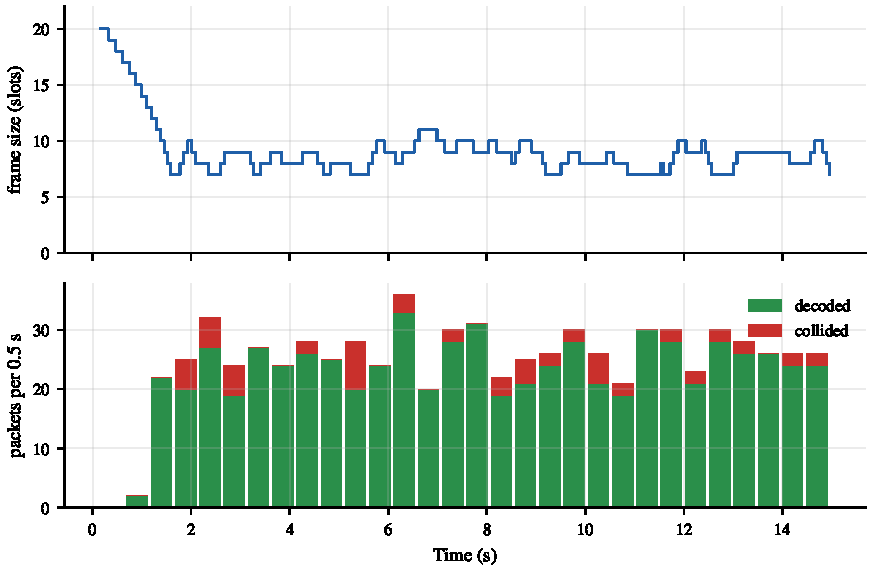
\includegraphics[width=0.82\linewidth]{fig_adaptation}
\caption{Adaptive framed-slotted ALOHA over $\SI{15}{s}$ (from the repository's committed output). Top: frame size per frame; it collapses from $20$ to about $8$ within $\SI{1.5}{s}$ as the BS learns how few nodes are contending. Bottom: decoded and collided packets per $\SI{0.5}{s}$ bin.}
\label{fig:adaptfig}
\end{figure}

\paragraph{Dynamics.} For the first second no node has activated (they are charging), so frames are empty and the policy shrinks the frame by one slot per frame ($20\to7$). From $\SI{0.8}{s}$ nodes start answering; the frame size settles around $S\approx8.4$ with an average of $3.9$ contenders per frame ($3.6$ decoded, $0.3$ collided). Only $\approx4$ of the $12$ nodes contend in any frame: the others are charging, or sit the frame out because of the look-ahead effect of Chapter~\ref{ch:bsengine}.

\paragraph{Collisions are rarer than ALOHA predicts.} With $n=3.9$, $S=8.4$ the textbook probability that a given node's slot is shared is $1-(1-1/S)^{n-1}\approx31\%$. The measured collided share is $8\%$. The difference is due to (i) capture and SIC resolving most pairs (the nodes' powers span $\SI{-66.7}{dBm}$ to $\SI{-14.6}{dBm}$), and (ii) the $5$~ms rule, which lets same-slot packets that start $\ge6$~ms apart coexist.

\paragraph{A surprising fairness result.}
The per-node decoded counts are very uneven:
\begin{center}
\small
\renewcommand{\arraystretch}{1.1}
\begin{tabular}{@{}rrrr|rrrr@{}}
\toprule
node & $r$ (m) & $P_{\mathrm{dl}}$ (mW) & decoded & node & $r$ (m) & $P_{\mathrm{dl}}$ (mW) & decoded\\
\midrule
 3 & 7.0 & 32.6 & \textbf{94} &  0 & 16.3 & 0.63 & 41\\
 4 & 6.3 & 8.2 & \textbf{95} &  1 & 27.8 & 0.11 & 41\\
 5 & 7.4 & 6.1 & \textbf{90} &  2 & 23.8 & 0.33 & 40\\
 7 & 9.3 & 44.3 & \textbf{77} &  6 & 19.9 & 0.63 & 41\\
 \multicolumn{4}{c|}{} & 8,9,10,11 & 25--39 & 0.1--0.8 & 42--44\\
\bottomrule
\end{tabular}
\end{center}
Eight nodes decode an almost identical $40$--$44$ packets, and four decode about twice as many. Both facts follow from the theory.
\begin{enumerate}
 \item The eight ``ordinary'' nodes receive less RF power than the solar trace delivers ($\SI{1.43}{mW}$). With \codew{combine_mode="max"} their energy source is the \emph{same} solar trace, so they have identical energy budgets and, in an uncongested system, identical rates: \emph{energy-limited throughput} (Chapter~\ref{ch:protocols}).
 \item The four ``rich'' nodes lie within $10$~m of the mast, where the RF power ($6$--$\SI{44}{mW}$) \emph{exceeds} the solar power by up to $30\times$, so the max-rule makes RF their source and they recharge much faster.
\end{enumerate}
But $\SI{44}{mW}$ at $\SI{9.3}{m}$ is $+16.5$~dBm, absurdly high for a $\SI{46}{dBm}$ transmitter with a $\SI{25}{m}$ mast: it is the \emph{\textless{}10~m path-loss artefact} of Chapter~\ref{ch:pathloss} (UMa falls through to its second branch and understates the loss by $\sim\SI{14}{dB}$). This is an excellent worked example of how a numerical edge case in the channel propagates, through the energy model, into a protocol-level fairness result. \textbf{The unevenness is not a property of adaptive ALOHA; it is a property of a path-loss branch.} The base station's frame adaptation is working correctly in both cases.

\section{The paper's experiment}
\label{sec:paperexp}

We summarised the experiment and our re-creation in Chapter~\ref{ch:protocols}. Here are practical notes for reading its Figure~2.
\begin{itemize}
 \item The figure is a \emph{box plot}: for each node count, the box spans the interquartile range of the $10$ runs, the centre line (or marker) the median, whiskers the range of non-outliers, dots the outliers. The wide boxes at low density ($\sim80$--$100\%$) reflect the discrete nature of small populations (with $5$ nodes, one failure is $20$ percentage points).
 \item A faithful reproduction needs the \emph{discovery frame parameters}: slot count, slot length, number of rounds, how nodes choose subcarrier shifts, and thresholds/electrical constants; none is given in the abstract. We therefore reproduce \emph{mechanisms}: monotone decay, effect of SIC, role of participation.
 \item With three base stations, a node may be heard by several; the paper's registration counts presumably count a node once. In Amber, ACKs are per base station (each \code{BSBehavior} has its own lists), so you must merge \codew{nodes_registered} across stations.
\end{itemize}

\section{Things to try}

Each is a one-line change that tests a piece of theory.
\begin{enumerate}
 \item \textbf{Capacitance.} Double $C$: the window $\Delta E$ doubles, charge cycles lengthen, packets per cycle rise but the long-run rate (duty-cycle theorem) barely changes.
 \item \textbf{Efficiency $\eta$.} Lower it from $0.7$ to $0.2$: every uplink weakens by $5.4$~dB; the margin of the $\SI{100}{m}$ node over the $\SI{-100}{dBm}$ sector sensitivity shrinks from $31$ to $26$~dB, and its collisions with stronger nodes become harder to resolve.
 \item \textbf{Remove the solar source.} Set \codew{node_energy_mode="wpt"} for all nodes: Node~2 never activates.
 \item \textbf{Move nodes beyond $\SI{10}{m}$} in the custom demo and watch the fairness gap close.
 \item \textbf{Sector power.} Reduce power by $10$~dB; the downlink of Node~1 falls from $-1$ to $\SI{-11}{dBm}$, its $V_\infty$ below $\Vhigh$: it stops.
 \item \textbf{Seeds.} Run any demo ten times and report mean $\pm$ s.d.
\end{enumerate}

\section{Chapter summary}
\begin{itemize}
 \item A five-row budget table (distance, $P_{\mathrm{dl}}$, source voltage, activation time, uplink RSSI) predicts the demos' outcome: who sends how often (by energy source) and who loses collisions (by received power).
 \item The three-node demos are deterministic functions of the budget plus random start-up delays; ten-seed means are the right basis for comparison.
 \item In the adaptive-ALOHA demo only $\sim4$ of $12$ nodes contend per frame; collisions are rarer than textbook ALOHA predicts because of capture, SIC and the $5$~ms rule.
 \item Per-node unevenness in that demo is traced to the $<\SI{10}{m}$ path-loss artefact and the max-rule of hybrid mode, not to the protocol.
\end{itemize}

\section*{Exercises}
\begin{exercise}
Rebuild the budget table for the unicast demo's SIC variant ($30^\circ$ beamwidth). Does the $30^\circ$ beam change any node's gain? (All nodes lie on the boresight.)
\end{exercise}
\begin{exercise}
Using the measured source voltages, estimate the ratio of packets sent by Node~0 and Node~1 from the duty-cycle theorem and compare with $46:18$. Which assumption of the theorem is most violated?
\end{exercise}
\begin{exercise}
In the custom demo, the frame size converges to $\approx8.4$ slots with $\approx3.9$ contenders. Evaluate the slot efficiency of this operating point, and compare it with the $S=n$ and $S=2n$ cases of Section~\ref{sec:energytwist}.
\end{exercise}
\begin{exercise}
Design a ten-seed experiment that isolates the effect of the $<\SI{10}{m}$ artefact on the custom demo's throughput (hint: compare node positions drawn from $[5,40]$ and from $[10,40]$).
\end{exercise}

\chapter{Extending Amber: Writing Your Own Protocol}
\label{ch:extending}

\begin{defbox}[In this chapter you will learn]
\begin{itemize}
 \item how the adaptive-ALOHA demo implements a complete user protocol with two small pieces of code and no engine changes;
 \item how to write and evaluate a new base-station policy, through a measured case study of \emph{energy-aware polling};
 \item a checklist for building experiments, and a gallery of the commonest mistakes with their symptoms;
 \item where the model invites extension.
\end{itemize}
\end{defbox}

\section{Anatomy of a user protocol: adaptive ALOHA}
\label{sec:anatomy}

The shipped \codew{custom_protocol} demo is the template for everything in this chapter. Its docstring states the contract: ``Nothing in Amber's engine is edited.'' It consists of a \emph{node half} and a \emph{base-station half}.

\subsection{Node half}
We met it in Chapter~\ref{ch:bsmodule}: subclass \codew{BackscatterModule} and override two methods.
\begin{lstlisting}
class AdaptiveAlohaNode(backscatter.BackscatterModule):
    def handle_command(self, cmd, bs_id, data):
        if cmd == "collect":              # my protocol's one command
            self.chosen_slot_idx = (random.randint(0, len(self.rx_slots) - 1)
                                    if self.rx_slots else -1)
            self.state = "active"
            self.last_tx_command_time = self.env.now

    def build_tx_payload(self, sensor_data):
        return ({"type": "data", "payload": sensor_data}
                if self.state == "active" else None)
\end{lstlisting}
The protocol vocabulary is whatever strings you choose for \code{cmd} (here ``\code{collect}''). There is no registration phase: the first \code{collect} activates a node. The framework supplies the sensitivity gate, the slot validity checks and the uplink.

\subsection{Base-station half}
The policy is a generator that yields one frame at a time and adapts between frames.
\begin{lstlisting}
def adaptive_aloha_policy(bs):
    n_slots, prev_collided, load_ema = START_SLOTS, 0, 0.0
    while True:
        yield [("tx", 5, "collect", {"cmd": "collect", "target": -1})] + \
              [("rx", 8, "slot") for _ in range(n_slots)]
        # execution resumes here after the whole frame has played out
        heard = len(bs.decoded_this_frame)
        collided = bs.total_collided - prev_collided
        prev_collided = bs.total_collided
        load_ema = 0.75 * load_ema + 0.25 * (heard + collided)
        target = min(MAX_SLOTS, max(MIN_SLOTS, round(2 * load_ema)))
        if n_slots < target:       n_slots += 1
        elif n_slots > target + 1: n_slots -= 1
\end{lstlisting}
Read it as a controller. The \emph{measurement} is the number of contenders $m=\text{heard}+\text{collided}$ in the last frame; it is smoothed with an exponential moving average ($\alpha=0.25$) to avoid chasing noise; the \emph{set-point} is $S^\star=2\ell$ (Section~\ref{sec:energytwist}), clamped to $[2,32]$; the \emph{actuator} moves $S$ by at most one per frame, with a one-slot dead band above the target (so $S$ does not oscillate around the target). \textbf{Command and slots are yielded in the same frame}, a requirement of the look-ahead (Chapter~\ref{ch:bsengine}).

\subsection{Wiring}
\begin{lstlisting}
nodes_modules = [AdaptiveAlohaNode(env=env, node=n, bs_processes=[],
                                   uplink_results=ul, downlink_results=dl)
                 for n in nodes]
bs_behavior = bsengine.BSBehavior(env=env, base_station=bs,
                                  policy=adaptive_aloha_policy,
                                  backscatter_modules=nodes_modules,
                                  enable_sic=True)
for m in nodes_modules: m.bs_processes = [bs_behavior]
\end{lstlisting}
Everything else (capacitors, controllers, coverage maps) is identical to the other demos (Chapter~\ref{ch:architecture}).

\section{Case study: does energy-aware polling help?}
\label{sec:pollcase}

\paragraph{The hypothesis.}
In Chapter~\ref{ch:protocols} we argued that a collision-free polling network is \emph{energy-limited}: the base station polls faster than nodes can recharge, so most polls fall on sleeping nodes ($\approx91\%$ in the three-node unicast demo). A natural optimisation is to \emph{avoid polling nodes that just failed to answer}: they are probably recharging. If throughput were limited by airtime, this should help substantially; if it is limited by harvested energy, it cannot help much. This is a clean test of the claim.

\paragraph{The policies.} Both are written as base-station policies on the unmodified engine. A frame is one poll: \texttt{("tx", 5, "poll", \{"cmd": "send\_data", "target": i\})} followed by \texttt{("rx", 10, "slot", \{"expect": i\})}, i.e.\ $\SI{15}{ms}$ per poll, so the airtime budget is $\lfloor20\,001/15\rfloor=1333$ polls in $\SI{20}{s}$ for \emph{both} policies.
\begin{lstlisting}
def policy(bs):                       # skip_silent (penalty = P polls)
    skip = {i: 0 for i in range(N)}; i = 0
    while True:
        if skip[i] > 0:               # recently silent: leave it alone
            skip[i] -= 1; i = (i + 1) % N; continue
        yield [("tx", 5, "poll", {"cmd": "send_data", "target": i}),
               ("rx", 10, "slot", {"expect": i})]
        if i not in bs.decoded_this_frame:     # no answer -> penalise
            skip[i] = P
        i = (i + 1) % N
\end{lstlisting}
\emph{Round-robin} is the same without the \code{skip} logic. Scenario: $N=12$ registered nodes, hybrid energy mode with the solar trace, placed uniformly at random in an annulus $r\in[10,40]$~m (to stay clear of the $<\SI{10}{m}$ artefact), $\eta=0.7$, the demo electrical parameters, $\SI{20}{s}$ horizon, SIC on; $10$ seeds per policy (script \file{textbook/code/polling_experiment.py}).

\begin{table}[t]
\centering
\small
\caption{Round-robin versus skip-silent polling, $N=12$ nodes, $\SI{20}{s}$, mean over $10$ seeds. Paired differences use the same seeds.}
\label{tab:polling}
\renewcommand{\arraystretch}{1.1}
\begin{tabular}{@{}lrrrrr@{}}
\toprule
Policy & Decoded & Polls & Decoded/poll & Throughput & Gain vs RR\\
\midrule
round-robin & $667.2$ & $1333$ & $0.501$ & $33.4$ pkt/s & --\\
skip, penalty $2$ & $684.7$ & $1333$ & $0.514$ & $34.2$ pkt/s & $+2.6\%$ ($t=11.6$)\\
skip, penalty $4$ & $683.6$ & $1333$ & $0.513$ & $34.2$ pkt/s & $+2.5\%$ ($t=8.1$)\\
skip, penalty $8$ & $680.6$ & $1333$ & $0.511$ & $34.0$ pkt/s & $+2.0\%$ ($t=5.4$)\\
skip, penalty $16$ & $679.5$ & $1333$ & $0.510$ & $34.0$ pkt/s & $+1.8\%$ ($t=4.2$)\\
\bottomrule
\end{tabular}
\end{table}

\paragraph{Result.}
Skipping silent nodes helps, but only by $\approx2$--$3\%$: small, yet statistically solid ($t$ between $4$ and $12$ in the paired comparison). Half of all polls are answered even by round-robin, and the smartest policy we tried answers $51.4\%$. Each node decodes about $55$--$60$ packets in $\SI{20}{s}$ ($\approx2.8$ per second) whatever the policy; the total $\approx34$~pkt/s is \emph{half of the airtime capacity of} $1333/20=66.7$ polls/s.

\paragraph{Interpretation.}
The hypothesis was right in the way that matters: the policy cannot beat the energy bound, because the number of packets a node can send is set by how fast its capacitor refills, not by which polling order the base station uses. All the policy decides is \emph{which node spends its next burst now}; avoiding sleepers saves airtime but airtime was not scarce. Think of the nodes as taps filling buckets at fixed rates: re-ordering how you visit the taps does not increase the water you collect per hour. To move the needle one must change the \emph{energy side}: better harvesting, a larger $C$ or lower $\Vlow$ (longer bursts), lower per-packet energy, or a transmission cap that respects the duty-cycle theorem. This is exactly the sort of conclusion a simulator that couples energy and protocol is built to expose.

\begin{reality}[Interpret small effects with care]
We changed one thing; the policies share seeds, so the paired comparison removes most of the placement variance. Nevertheless the node population is homogeneous (identical sources), the poll order is rigid, and the model's energy accounting has the caveats of Chapter~\ref{ch:capacitor} (over-credited harvesting while active, brown-out truncation). The qualitative conclusion---\emph{energy dominates}---is robust to these; the $2.6\%$ is specific to this configuration.
\end{reality}

\section{A checklist for new experiments}
\label{sec:checklist}

\begin{enumerate}
 \item \textbf{State the question} and the metric (Chapter~\ref{ch:analysis}); decide what you will compare against.
 \item \textbf{Fix the scenario} (geometry, power, energy mode, electrical parameters) in one config; keep nodes $\ge\SI{10}{m}$ from masts.
 \item \textbf{Make runs reproducible}: seed Python's \code{random}; log the seed.
 \item \textbf{Wire the eight steps} of Chapter~\ref{ch:architecture}; set \codew{bs_processes}.
 \item \textbf{Warm up}: nodes need $\approx2$--$4$~s to charge and the start-up delay is up to $2$~s; start protocol measurements after that or account for it.
 \item \textbf{Keep the base-station process alive} (long final window).
 \item \textbf{Replicate}: $\ge10$ seeds, report mean and spread; use \emph{paired} seeds when comparing designs.
 \item \textbf{Change one factor at a time}; the shipped demos change six.
 \item \textbf{Sanity-check with theory}: a link-budget table, an RC charge time, an ALOHA estimate. If the simulator disagrees, find out why before trusting it.
 \item \textbf{Record the caveats} of Chapter~\ref{ch:limits} that apply to your result.
\end{enumerate}

\section{A gallery of mistakes}
\label{sec:mistakes}

\begin{center}
\small
\renewcommand{\arraystretch}{1.15}
\begin{tabularx}{\linewidth}{@{}>{\raggedright}p{4.1cm}>{\raggedright}X>{\raggedright\arraybackslash}p{4.3cm}@{}}
\toprule
\textbf{Symptom} & \textbf{Likely cause} & \textbf{Fix}\\
\midrule
Nodes ``transmit'' (TX records exist) but the base station logs nothing & \codew{bs_processes} never set (Step~7) & \codew{m.bs_processes=[beh]} for every module\\
\codew{RuntimeError: ... has terminated and cannot be interrupted} & base-station process ended (\code{loop=False}, exhausted policy) while nodes hold slots & end with a long idle RX window\\
\codew{AttributeError: harvesting_power_dbm} & controller built before \codew{calculate_node_power} & call it before creating controllers\\
Nodes never activate & $V_\infty<\Vhigh$ (RF only, too far, or too little power) & compute Eq.~\eqref{eq:tauvinf}; add an external source\\
Registration stalls at $\approx$half per round & two-frame look-ahead & expect factor $\tfrac12$; use more rounds or slots\\
\code{send_data} to a list gets no replies & default handler ignores list targets & override \codew{handle_command}\\
Changing \code{R_series} changes nothing & controller uses a hard-coded $\SI{5}{k\ohm}$ lookup & set both places, or patch the lookup\\
Different results on each run & unseeded randomness & \codew{random.seed(...)}\\
Memory grows without bound & \codew{keep_logs=True} & \codew{keep_logs=False}, \code{stream_log}\\
Odd extra throughput for nodes near the mast & $<\SI{10}{m}$ path-loss branch & keep nodes $\ge\SI{10}{m}$\\
\codew{analyze_packets} says 1 of 124 packets decoded & zero-length-interval defect in post-hoc detection & use the engine's \code{collided} flags\\
\bottomrule
\end{tabularx}
\end{center}

\section{Where the model invites extension}

The architecture makes the following research directions natural; each is a replacement of one module behind the contracts of Section~\ref{sec:contracts}.
\begin{itemize}
 \item \textbf{A realistic harvester}: an RF--DC efficiency curve with a turn-on threshold and cold-start (replace the conversion in \codew{calculate_node_power}).
 \item \textbf{Imperfect SIC}: add the decoded packets' residual to the interference sum (Chapter~\ref{ch:sic}).
 \item \textbf{Energy-causal transmissions}: refuse to start a burst the capacitor cannot finish, or count truncated bursts as failures (Chapter~\ref{ch:controller}).
 \item \textbf{Fading and shadowing}: replace the constant link budget with a per-packet random draw (this requires giving up the one-time pre-computation).
 \item \textbf{Mobility}: recompute channel entries as nodes move, or per slot.
 \item \textbf{Wake-up receivers} and non-zero idle current in \emph{wait\_slot}.
 \item \textbf{Smarter protocols}: energy-state reporting, schedule prediction from the node's recharge time, multi-carrier or multi-reader cooperation.
\end{itemize}

\section{Chapter summary}
\begin{itemize}
 \item A complete protocol is a node subclass (two methods) plus a base-station policy generator.
 \item The energy-aware polling case study improved decoded packets by only $\approx2$--$3\%$ because throughput is bounded by harvested energy.
 \item A short checklist and a table of symptoms and causes will save hours.
 \item The module contracts of Chapter~\ref{ch:architecture} define where extensions plug in.
\end{itemize}

\section*{Exercises}
\begin{exercise}
Implement a node protocol in which the node replies only if it received the command with at least $\SI{3}{dB}$ margin over its sensitivity, and justify the rule physically.
\end{exercise}
\begin{exercise}
Modify the polling policy so that the penalty grows exponentially with consecutive silent polls (exponential back-off). Predict, using the duty-cycle theorem, whether this can exceed the $\approx34$~pkt/s bound.
\end{exercise}
\begin{exercise}
Write a base-station policy that alternates a discovery frame and a polling round and stops discovering once all $N$ nodes are registered. List the \code{BSBehavior} attributes you read.
\end{exercise}
\begin{exercise}
Add a rule so that a node starts a transmission only if $V\ge\Vlow+\Delta V_{\mathrm{burst}}$. How would you obtain the voltage in the node protocol given the contracts?
\end{exercise}

\chapter{Assumptions, Limits and Verified Caveats}
\label{ch:limits}

\begin{defbox}[In this chapter you will learn]
\begin{itemize}
 \item a catalogue of every modelling assumption and code behaviour discussed in the book, in one place, each with the evidence for it;
 \item which ones can change a headline result and which are cosmetic;
 \item a checklist of validity questions to ask of any Amber result;
 \item where to go next.
\end{itemize}
\end{defbox}

\paragraph{How to read this chapter.} Amber is version~0.1.0 of a research prototype, described by a two-page demo abstract. It is natural for such a tool to contain simplifications and rough edges, and the authors state its scope honestly. The point of cataloguing them is not criticism but \emph{calibration}: you should know which results you may trust. Each row below states the behaviour, the \textbf{evidence} (\emph{measured}: we ran an experiment; \emph{tested}: a targeted test of the code; \emph{read}: established by reading the source), and the \textbf{effect}. We did \emph{not} modify the Amber source in preparing this book.

\section{Catalogue}

\newcommand{\sev}[1]{\textbf{#1}}
\setlength{\LTleft}{0pt}\setlength{\LTright}{0pt}
\renewcommand{\arraystretch}{1.12}

\subsection{Channel and radio}
\begin{longtable}{@{}>{\sffamily\bfseries}p{0.9cm}>{\raggedright}p{5.5cm}>{\raggedright}p{2.9cm}>{\raggedright\arraybackslash}p{5.2cm}@{}}
\toprule
\# & Behaviour & Evidence & Effect (severity)\\
\midrule
\endhead
R1 & UMa LOS falls through to the post-breakpoint branch for $d_{2D}<\SI{10}{m}$: a $\SI{13.8}{dB}$ step at $\SI{10}{m}$ (Ch.~\ref{ch:pathloss}) & \emph{tested}: 44.4 vs 58.3 dB at 9.99/10 m & Nodes $<10$~m get $\sim14$~dB too much RF; produced $2\times$ throughput for 4 of 12 nodes in the custom demo (Ch.~\ref{ch:experiments}). \sev{High} near masts\\
R2 & FSPL mode uses $d_{2D}$ not $d_{3D}$ & \emph{tested} & 14 dB error at 5 m, 0.2 dB at 100 m. \sev{Low}\\
R3 & Horizontal antenna pattern only; no downtilt (Ch.~\ref{ch:antennas}) & \emph{read} & Overestimates gain for nodes close to the mast. \sev{Medium} near masts\\
R4 & Deterministic static channel: no fading, shadowing, mobility & \emph{read} (by design) & Realistic variability absent; results are optimistic and smooth. \sev{Design scope}\\
R5 & A node harvests the best sector only; no carrier summation or inter-cell interference & \emph{read} (Ch.~\ref{ch:coverage}) & Conservative for energy; no downlink interference. \sev{Low}--\sev{Medium}\\
R6 & \codew{CoverageMap.bandwidth_hz}, \codew{noise_figure_db} unused & \emph{read} (grep) & Cosmetic; noise comes from the base station's own arguments. \sev{Low}\\
R7 & Sensitivity thresholds are independent of the noise floor; with default 100 MHz the noise ($-88$ dBm) exceeds sector sensitivity ($-100$ dBm) & \emph{read}, \emph{tested} & Set both consistently. \sev{Medium}\\
R8 & A lone packet above sensitivity is decoded regardless of SNR; noise enters only collisions & \emph{tested}: $-105$ dBm, SNR $-17$ dB decoded & Weak-link PER is not modelled. \sev{Medium}\\
R9 & Command reception uses the best power over \emph{all} base stations, not the sender's & \emph{read} & Multi-BS command coverage is optimistic. \sev{Low}\\
R10 & Subcarrier shifts are perfectly orthogonal; no carrier leakage or sideband loss (Ch.~\ref{ch:backscatter}) & \emph{read} & Self-interference---the central practical backscatter issue---is not simulated. \sev{Design scope}\\
\bottomrule
\end{longtable}

\subsection{Energy and node behaviour}
\begin{longtable}{@{}>{\sffamily\bfseries}p{0.9cm}>{\raggedright}p{5.5cm}>{\raggedright}p{2.9cm}>{\raggedright\arraybackslash}p{5.2cm}@{}}
\toprule
\# & Behaviour & Evidence & Effect (severity)\\
\midrule
\endhead
E1 & No RF--DC efficiency curve, turn-on threshold or cold start (Ch.~\ref{ch:harvest}) & \emph{read} & Energy availability is optimistic at low RF power. \sev{High} for RF-limited studies\\
E2 & Controller converts power to voltage with \codew{getattr(cap,"R_series",5e3)}, which always returns $5\,\mathrm{k}\Omega$ & \emph{tested} & Changing $R_s$ in \codew{CapacitorParams} silently mismatches the source voltage. \sev{Medium} (latent)\\
E3 & Charge-and-discharge step credits $\Vs I\Delta t$ (source energy), not $V I\Delta t$ (delivered): over-credit by $\Vs/V$ & \emph{tested}, \emph{measured}: $\SI{1.948}{V}$ vs $\SI{1.695}{V}$ after 1 s; $-2.7\%$ packets when corrected & Harvest overstated while active. \sev{Medium}\\
E4 & Packet is delivered at \emph{entry} to the transmit state; the energy is paid afterwards. $43$--$50\%$ of transmit states end in brown-out & \emph{measured} (3 nodes, 20 s) & Delivered counts are optimistic by up to $\sim2\times$ under tight energy budgets. \sev{High}\\
E5 & \emph{wait\_slot} draws zero current & \emph{read} & Idle/wake-up-receiver cost ignored. \sev{Medium}\\
E6 & Energy gates transmission, not reception; protocol state survives power-down & \emph{tested}: module with no capacitor accepts commands & Registration/slot state of ``dead'' nodes changes; real nodes would hear nothing. \sev{Medium}\\
E7 & Shipped solar trace is $2999$ rows $=\SI{3}{s}$, looped; file named ``300 seconds''; shared by all nodes & \emph{measured} & Spurious periodicity possible; no spatial shading. \sev{Low}\\
E8 & \codew{Capacitor.load_discharging} / cause \codew{capacitor_discharge} never used by the shipped controller & \emph{read} (grep) & Dead code path. \sev{Cosmetic}\\
E9 & Demo loads ($\sim\SI{5}{mA}$) are $10^3$--$10^4\times$ above Release-19 $\sim\SI{1}{\micro W}$ targets & \emph{read} & Demos are not representative of ultra-low-power tags. \sev{Interpretation}\\
\bottomrule
\end{longtable}

\subsection{MAC, SIC and software}
\begin{longtable}{@{}>{\sffamily\bfseries}p{0.9cm}>{\raggedright}p{5.5cm}>{\raggedright}p{2.9cm}>{\raggedright\arraybackslash}p{5.2cm}@{}}
\toprule
\# & Behaviour & Evidence & Effect (severity)\\
\midrule
\endhead
M1 & \codew{cancellation_factor} has no effect: SIC is perfect cancellation (Ch.~\ref{ch:sic}) & \emph{tested}: identical decode sets for several $\kappa$ from $0$ to $1$ & Imperfect SIC not simulated; SIC gain overstated. \sev{High} for SIC studies\\
M2 & Collision = arrival within $\SI{5}{ms}$ (greedy, non-transitive), packets have no duration & \emph{tested}: $10,14,18$ ms $\Rightarrow$ third packet escapes & Collision statistics are model-dependent. \sev{Medium}\\
M3 & Advertised RX slots cover \emph{two} frames; random pick over $2S$ $\Rightarrow$ $\approx\frac12$ participation per frame (Ch.~\ref{ch:bsengine}) & \emph{tested}: 8 advertised for a 4-slot frame; \emph{measured}: 44/70/82/88\% registered over rounds at $n=5$ & Slows discovery by $\sim2\times$ per round; must be budgeted. \sev{High} for MAC studies\\
M4 & \codew{TxRecord.delivered} is True when handed to any BS process; $-150$ dBm packet is ``delivered'' & \emph{tested} & Not a delivery metric. \sev{Medium}\\
M5 & \code{send_data} with a list \code{target} accepted by BS, ignored by default node handler & \emph{tested} & Multicast silently fails. \sev{Low}\\
M6 & ACK is a direct call, always received; BS marks registered at send & \emph{read} & Real ACK loss absent. \sev{Medium}\\
M7 & A terminated BS process makes a later node transmission raise \codew{RuntimeError} & \emph{tested} (crash reproduced) & Aborts the simulation. \sev{Medium} (usability)\\
M8 & ``DER'' means error rate in demos, success ratio in \code{BSStats.der} & \emph{read}, \emph{tested} & Easy to misreport. \sev{Medium}\\
M9 & Post-hoc \codew{detect_collisions} mislabels almost all packets on engine logs (zero-length intervals) & \emph{tested}: 1 vs 121 decoded; repaired: 120 & Only affects logs without \code{collided}. \sev{Medium}\\
M10 & \codew{analyze_packets} appends text files to the working directory; rejects demo CSVs & \emph{read}, \emph{tested} & Side effects; unusable on demo output. \sev{Low}\\
M11 & Randomness is unseeded by default (only the custom demo seeds) & \emph{read} & Run-to-run variation; replicate. \sev{Medium}\\
\bottomrule
\end{longtable}

\section{Which caveats matter for which question?}

\begin{center}
\small
\renewcommand{\arraystretch}{1.15}
\begin{tabularx}{\linewidth}{@{}>{\raggedright}p{4.8cm}X@{}}
\toprule
If your question concerns\ldots & Check first\ldots\\
\midrule
Absolute throughput / delivery & E4, E3, E1, R1, M4\\
Registration / discovery speed & M3, M2, M6, E6\\
SIC / collision resolution & M1, M2, R8, R10\\
Energy-limited operation, duty cycle & E3, E4, E5, E2, E7\\
Coverage and range & R1--R5, R7\\
Relative protocol comparison under identical assumptions & usually robust; replicate (M11) and use paired seeds\\
\bottomrule
\end{tabularx}
\end{center}

\section{Ten validity questions for any simulation result}
\label{sec:validityq}

\begin{enumerate}
 \item Is the result a \emph{comparison} under shared assumptions, or an \emph{absolute} number? (Prefer the former.)
 \item How many seeds, and what is the spread?
 \item Do the nodes at the edge of the scenario sit in a region where the channel model is valid ($d_{2D}\ge\SI{10}{m}$)?
 \item Is the source of each node's energy what you think it is (RF, solar, max, sum)?
 \item Is throughput limited by energy, by airtime or by collisions? Does a hand calculation agree?
 \item Does ``delivered'' mean decoded at a base station? Counted before or after the energy was paid?
 \item Are SIC and capture assumptions realistic for your receivers?
 \item Did you change one factor at a time?
 \item Could the effect you see come from the $5$~ms rule, the look-ahead or the node's start-up delay rather than the mechanism you study?
 \item Would the conclusion survive a $\pm3$~dB change in the link budget and a $\pm30\%$ change in the harvest?
\end{enumerate}

\section{Where to go next}

\begin{itemize}
 \item \textbf{Standards:} 3GPP TR~38.848, TR~38.769, TS~38.191 \citep{3gpp38848,3gpp38769,3gpp38191}; the channel model TR~38.901 \citep{3gpp38901}.
 \item \textbf{Overview:} L\'opez et al.\ \citep{lopez2025zero}; the backscatter survey of Huynh et al.\ \citep{huynh2018ambient}; the dual-tone downlink idea \citep{zhu2022ofdma}.
 \item \textbf{Textbooks:} Dobkin on UHF RFID \citep{dobkin2012}; Tse and Viswanath for SIC and multiple access \citep{tse2005}; Banks et al.\ or Law for simulation methodology \citep{banks2010,law2015}.
 \item \textbf{The simulator:} the repository, the generated API reference from the docstrings, and the SenSys demo abstract \citep{manafova2026amber}.
 \item \textbf{Your own experiments:} Chapter~\ref{ch:extending}, with the scripts in \file{textbook/code}.
\end{itemize}

\section{Chapter summary}
\begin{itemize}
 \item We catalogued $10$ channel/radio, $9$ energy/node and $11$ MAC/software behaviours, each with its evidence.
 \item The most consequential for headline numbers: brown-out truncation (E4), perfect SIC (M1), the two-frame look-ahead (M3), the $<10$~m path-loss branch (R1) and the missing RF--DC curve (E1).
 \item Relative comparisons under identical assumptions are the safest use of the simulator; always replicate.
\end{itemize}

\section*{Exercises}
\begin{exercise}
Pick any \emph{High} item and propose a minimal code change that removes it. State what you would measure to show the change had the intended effect.
\end{exercise}
\begin{exercise}
A paper reports ``Amber shows SIC raises throughput by $40\%$''. List the three caveats from this chapter you would check first, and the experiment you would run.
\end{exercise}
\begin{exercise}
Using the validity questions, critique the claim ``the adaptive ALOHA policy gives node $4$ twice the throughput of node $1$ because it is better located''.
\end{exercise}


\appendix
\chapter{Derivations}
\label{app:derivations}

This appendix gathers, in compact but complete form, derivations that the main text states or sketches.

\section{Solution of the capacitor equation}
\label{app:rc}

Equation~\eqref{eq:ode}: $C\dot V=(\Vs-V)/\Rs-V/\Rl-I_L$. Collect the terms in $V$:
\[
 C\dot V+\Big(\frac1{\Rs}+\frac1{\Rl}\Big)V=\frac{\Vs}{\Rs}-I_L
 \quad\Longrightarrow\quad
 \dot V+\frac V\tau=\frac{V_\infty}{\tau},
\]
with $\tau=C/(1/\Rs+1/\Rl)=(\Rs\parallel\Rl)C$ and $V_\infty=\tau(\Vs/\Rs-I_L)/C=(\Vs-I_L\Rs)\,\Rl/(\Rl+\Rs)$. Multiplying by the integrating factor $\e^{t/\tau}$:
\[
 \frac{\mathrm d}{\mathrm dt}\big(V\e^{t/\tau}\big)=\frac{V_\infty}{\tau}\e^{t/\tau}
 \ \Rightarrow\
 V(t)\e^{t/\tau}=V_0+V_\infty(\e^{t/\tau}-1)
 \ \Rightarrow\
 V(t)=V_\infty+(V_0-V_\infty)\e^{-t/\tau}.
\]
Setting $V(t_{\mathrm{th}})=V_{\mathrm{th}}$ and solving gives Eq.~\eqref{eq:tth}.

\paragraph{Discrete step.} Explicit Euler on the source term alone gives $V_{k+1}=V_k+\frac{\Delta t}{\Rs C}(\Vs-V_k)$, with amplification factor $1-\Delta t/(\Rs C)\in(0,1)$ when $\Delta t<\Rs C$ (stable, here $\Delta t/\Rs C=6.7\times10^{-4}$). Leakage alone is $V\to V\e^{-\Delta t/\Rl C}$ exactly. Composing them (Eq.~\eqref{eq:chargestep}) commits an $O(\Delta t^2)$ local error per step, hence $O(\Delta t)$ globally, with a coefficient of order $\Delta t/\tau\sim10^{-3}$: we measured an error of $1.7\times10^{-4}$ V after $\SI{1}{s}$.

\section{Maximum power into the capacitor}
Power into the capacitor through $\Rs$ at voltage $V$ is $p(V)=V(\Vs-V)/\Rs$. Then $p'(V)=(\Vs-2V)/\Rs=0$ at $V=\Vs/2$ and $p_{\max}=\Vs^2/(4\Rs)=P_h/4$, with $P_h=\Vs^2/\Rs$. Equivalently $p=P_h\,x(1-x)$, $x=V/\Vs$.

\section{Duty-cycle theorem}
See Section~\ref{sec:hysteresis}. With $T_c=\Delta E/P_{\mathrm{in}}$, $T_a=\Delta E/(P_{\mathrm{act}}-P_{\mathrm{in}})$: $D=T_a/(T_a+T_c)=P_{\mathrm{in}}/P_{\mathrm{act}}$, because
$\dfrac1{P_{\mathrm{act}}-P_{\mathrm{in}}}\Big/\Big(\dfrac1{P_{\mathrm{act}}-P_{\mathrm{in}}}+\dfrac1{P_{\mathrm{in}}}\Big)=\dfrac{P_{\mathrm{in}}}{P_{\mathrm{in}}+(P_{\mathrm{act}}-P_{\mathrm{in}})}$.

\section{Framed slotted ALOHA: slot statistics}
\label{app:fsa}

Each of $n$ nodes picks one of $S$ slots independently and uniformly. The occupancy $X$ of a given slot is Binomial$(n,1/S)$:
$\Pr[X=k]=\binom nk S^{-k}(1-1/S)^{n-k}$. Hence
$\Pr[X=0]=(1-1/S)^n$, $\Pr[X=1]=\frac nS(1-1/S)^{n-1}$. By linearity of expectation over the $S$ slots, $E_0=S\Pr[X=0]$, $E_1=S\Pr[X=1]=n(1-1/S)^{n-1}$ and $E_c=S-E_0-E_1$. A tagged node succeeds iff each of the other $n-1$ nodes avoided its slot: $(1-1/S)^{n-1}$.

\paragraph{Optimal frame size.} Let $r=n/S$. For large $S$, $(1-1/S)^{n-1}\to\e^{-r}$, so $\eta_S\to r\e^{-r}$, with $\mathrm d\eta_S/\mathrm dr=(1-r)\e^{-r}=0$ at $r=1$ and $\eta_S(1)=1/\e$.

\paragraph{Pure and slotted ALOHA.} A transmission starting at $t_0$ is vulnerable to any other start in $(t_0-T,t_0+T)$ (pure) or in the same slot (slotted). With Poisson arrivals of rate $g$ per packet time, the probability of no other start in an interval of length $2T$ (resp.\ $T$) is $\e^{-2g}$ (resp.\ $\e^{-g}$). The maximum of $g\e^{-2g}$ is at $g=1/2$ ($1/2\e$) and of $g\e^{-g}$ at $g=1$ ($1/\e$).

\section{SIC: the ratio rule}
\label{app:sicratio}

For perfect cancellation and negligible noise, powers $P_{(k)}=P_{(1)}\rho^{-(k-1)}$ with $\rho>1$. At stage $k$ the interference is the sum of all weaker packets: $P_{(k)}\sum_{j\ge1}\rho^{-j}$ for an infinite chain, which converges to $P_{(k)}/(\rho-1)$. Thus $\gamma_{(k)}=\rho-1$ for every $k$, and decoding all packets requires $\rho-1\ge\gamma_{\mathrm{req}}$, i.e.\ $\rho\ge1+\gamma_{\mathrm{req}}$ (in linear units). For a finite chain of $m$ packets the ratio at the last stages is larger, so $\rho\ge1+\gamma_{\mathrm{req}}$ is sufficient. With $\gamma_{\mathrm{req}}=3$~dB ($\approx2.0$) we need $\rho\ge3.0$ ($4.8$~dB). The strongest of four packets exceeds the weakest by $\rho^{3}=27$ ($14.3$~dB).

\section{Sidebands of a switched reflection}
\label{app:fourier}

Let $s(t)\in\{0,1\}$ be a unit square wave with period $1/f_s$ and 50\% duty. Its Fourier series is $s(t)=\tfrac12+\tfrac2\pi\sum_{k=1,3,5,\dots}\tfrac1k\sin(2\pi kf_st)$. The reflection coefficient is $\Gamma(t)=\Gamma_0+\Delta\Gamma\,s(t)$ and the reflected wave is $y(t)=\Gamma(t)\,A\cos(2\pi f_ct)$. Using $\sin a\cos b=\tfrac12[\sin(a+b)+\sin(a-b)]$ on the fundamental ($k=1$) term:
\[
 \Delta\Gamma\frac{2}{\pi}A\sin(2\pi f_st)\cos(2\pi f_ct)=\frac{\Delta\Gamma}{\pi}A\big[\sin 2\pi(f_c+f_s)t-\sin2\pi(f_c-f_s)t\big].
\]
Each sideband has amplitude $\Delta\Gamma A/\pi$, hence a power ratio of $(\Delta\Gamma/\pi)^2$ to the incident carrier ($A$). For $\Delta\Gamma=1$ this is $1/\pi^2=0.101$ ($-9.9$~dB); for $\Delta\Gamma=2$ it is $4/\pi^2=0.405$ ($-3.9$~dB). The constant term $\tfrac12\Delta\Gamma+\Gamma_0$ multiplies the carrier itself, giving the unshifted ``static'' reflection of Eq.~\eqref{eq:y0}.

\section{Friis in two lines}
Isotropic power density at range $d$: $S=P_tG_t/(4\pi d^2)$. Effective aperture of a receive antenna of gain $G_r$: $A_e=G_r\lambda^2/(4\pi)$ (a standard result obtained from antenna reciprocity and thermal equilibrium; see, e.g., \citet{pozar2011}). The received power is $S A_e=P_tG_tG_r(\lambda/4\pi d)^2$.

\section{3GPP UMa continuity at the breakpoint}
At $d_{2D}=d'_{BP}$ and ignoring the height difference in $d_{3D}$, $\mathrm{PL}_1=28+22\log d'_{BP}+20\log f_c$ and $\mathrm{PL}_2=28+40\log d'_{BP}+20\log f_c-9\log(d_{BP}'^{2}+\Delta h^2)\approx28+40\log d'_{BP}+20\log f_c-18\log d'_{BP}=28+22\log d'_{BP}+20\log f_c$ when $\Delta h\ll d'_{BP}$: the two branches agree, confirming the continuity claim. For the demo ($d'_{BP}=\SI{147.8}{m}$) we measured $75.17$ and $\SI{75.19}{dB}$ at $147.8$ and $\SI{148}{m}$.

\chapter{Formula and Parameter Reference}
\label{app:ref}

\section{Formula sheet}

\begin{center}
\small
\renewcommand{\arraystretch}{1.3}
\begin{tabularx}{\linewidth}{@{}>{\sffamily\bfseries}p{3.5cm}X@{}}
\toprule
Quantity & Formula\\
\midrule
dBm to W & $P=10^{(\Pdbm-30)/10}$\\
Link budget & $P_{\mathrm{rx}}=P_{\mathrm{tx}}+G_{\mathrm{tx}}-\mathrm{PL}+G_{\mathrm{rx}}$ (dB)\\
Thermal noise & $N=k_BT_0BF$; $-174+10\log B+\mathrm{NF}$ dBm\\
Friis & $P_r=P_tG_tG_r(\lambda/4\pi d)^2$; $\mathrm{PL}_{FS}=20\log(4\pi d/\lambda)$\\
3GPP sector gain & $G=G_{\max}-\min[12(\varphi/\varphi_{3\mathrm{dB}})^2,\,30]$\\
UMa LOS & $\mathrm{PL}_1=28+22\log d_{3D}+20\log f_c$ ($10\le d_{2D}\le d'_{BP}$); $\mathrm{PL}_2=28+40\log d_{3D}+20\log f_c-9\log(d_{BP}'^2+\Delta h^2)$\\
Breakpoint & $d'_{BP}=4(h_{BS}-1)(h_{UT}-1)f_c/c$\\
Backscatter uplink & $P_r=P_t+G_t+G_r+2G_a+10\log\eta-\mathrm{PL}(d_1)-\mathrm{PL}(d_2)$ (dB)\\
Harvest (WPT mode) & $P_h=P_{\mathrm{dl}}(1-\eta\,\mathbb 1_{\mathrm{tx}})$; $\Vs=\sqrt{P_h\Rs}$\\
Capacitor & $C\dot V=(\Vs-V)/\Rs-V/\Rl-I_L$; $V(t)=V_\infty+(V_0-V_\infty)\e^{-t/\tau}$\\
Steady state, $\tau$ & $V_\infty=(\Vs-I_L\Rs)\Rl/(\Rl+\Rs)$; $\tau=(\Rs\|\Rl)C$\\
Charge time & $t=\tau\ln[(V_\infty-V_0)/(V_\infty-V_{\mathrm{th}})]$\\
Energy window & $\Delta E=\tfrac12C(\Vhigh^2-\Vlow^2)$\\
Duty cycle & $D=P_{\mathrm{in}}/P_{\mathrm{act}}$\\
Slotted ALOHA & $s=g\e^{-g}$; FSA: $E_1=n(1-1/S)^{n-1}$, $P_{\mathrm{succ}}=(1-1/S)^{n-1}$\\
SINR & $\gamma_i=P_i/(\sum_{j\ne i}P_j+N)$; SIC: $\gamma_{(k)}=P_{(k)}/(\sum_{j>k}P_{(j)}+\varepsilon\sum_{j<k}P_{(j)}+N)$\\
Mean-field registration & $n_{k+1}=n_k-n_kp_a\,(1-p_a/SK)^{n_k-1}$\\
\bottomrule
\end{tabularx}
\end{center}

\section{Default values at a glance}

\begin{center}
\footnotesize
\renewcommand{\arraystretch}{1.12}
\begin{tabularx}{\linewidth}{@{}>{\ttfamily}p{3.2cm}>{\ttfamily}p{3.3cm}>{\ttfamily}p{2.1cm}X@{}}
\toprule
\normalfont\bfseries Parameter & \normalfont\bfseries Class & \normalfont\bfseries Default & \normalfont\bfseries Unit / note\\
\midrule
dt & CapacitorParams & 1e-3 & s (the simulator tick is 1 ms)\\
R\_series & CapacitorParams & 5e3 & $\Omega$ (the controller assumes 5e3)\\
R\_leakage & CapacitorParams & 0.1e6 & $\Omega$\\
C & CapacitorParams & 300e-6 & F\\
initial\_voltage & Capacitor & 0.0 & V\\
voltage\_max & Capacitor & 2.0 & V clamp\\
keep\_logs & Capacitor etc. & True & memory grows if True\\
max\_startup\_time\_ms & ControllerParams & 2000 & ms; delay uniform in $[0,\cdot)$\\
thresholds & VoltageThresholdsV & (set by user) & V; demo high 1.7, low 1.3\\
currents, durations & CurrentsA, DurationsMs & (set by user) & A, ms; demo in Ch.~\ref{ch:controller}\\
efficiency & Node & 1.0 & $\eta$\\
sensitivity\_dbm & Node & $-45$ & dBm\\
height & Node & 1.5 & m\\
antenna\_gain\_dbi & Node & 0.0 & dBi\\
subcarrier\_shift & Node & 0 & integer label\\
power & Sector & 43.0 & dBm\\
antenna\_gain\_dbi & Sector & 17.0 & dBi\\
height & Sector & 25.0 & m\\
sensitivity\_dbm & Sector & $-100$ & dBm\\
freq\_hz & CoverageMap & 925e6 & Hz\\
pathloss\_model & CoverageMap & "macro" & or "fspl"\\
node\_energy\_mode & CoverageMap & "wpt" & or "external", "hybrid"\\
combine\_mode & CoverageMap & "max" & hybrid combination\\
required\_sinr\_db & BSBehavior & 3.0 & dB\\
enable\_sic & BSBehavior & True & \\
cancellation\_factor & BSBehavior & 0.9 & \emph{inert}\\
noise\_figure\_db & BSBehavior & 6.0 & dB\\
bandwidth\_hz & BSBehavior & 100e6 & Hz\\
collision\_window\_ms & \_process\_rx\_buffer & 5.0 & ms (not a constructor argument)\\
resistance & EnvEnergySource & 1.0 & $\Omega$ (demos pass 5e3)\\
column & EnvEnergySource & "V\_IM" & trace column\\
\bottomrule
\end{tabularx}
\end{center}

\section{The demos' electrical and timing parameters}

\begin{center}
\small
\renewcommand{\arraystretch}{1.12}
\begin{tabular}{@{}lrl@{}}
\toprule
Item & Value & Source\\
\midrule
Carrier frequency & $\SI{924}{MHz}$ & all demos\\
Path loss & UMa LOS & all demos\\
Thresholds $\Vhigh/\Vlow$ & $1.7/\SI{1.3}{V}$ & all demos\\
$\Rs/\Rl/C$ & $5\,\mathrm{k}\Omega/100\,\mathrm{k}\Omega/\SI{300}{\micro F}$ ($\SI{200}{\micro F}$ in SIC demo) & demos\\
Listening & $5$ ms, $\SI{0.14}{mA}$ & demos\\
Sensing & $2$ ms, $\SI{0.512}{mA}$ & demos\\
Processing & $5$ ms, $\SI{1.28}{mA}$ & demos\\
Transmitting & $15$ ms, $\SI{5}{mA}$ & demos\\
TX command / RX slot & $5$ ms / $10$ ms ($15$ in SIC demo; $8$ in custom) & demos\\
Sector & $\SI{46}{dBm}$, $\SI{15}{dBi}$, azimuths $0^\circ,120^\circ,240^\circ$ & demos\\
Paper's experiment & $\SI{30}{dBm}$, $\SI{17}{dBi}$, nodes $\SI{1}{dBi}$ & paper\\
\bottomrule
\end{tabular}
\end{center}

\chapter{The Paper, Annotated}
\label{app:paper}

This appendix reads the SenSys demo abstract \citep{manafova2026amber} \emph{statement by statement}, linking each claim to the chapter that explains it, the code that implements it, and our verdict from reading and running the code. Quotations are from the paper. Verdict symbols: \textbf{\textcolor{agreen}{$\checkmark$}}~consistent with the code; \textbf{\textcolor{aorange}{$\sim$}}~consistent with caveats; \textbf{\textcolor{agrey}{$\circ$}}~an abstraction (described, not simulated at that level).

\section{Abstract and introduction}

\begin{center}
\footnotesize
\renewcommand{\arraystretch}{1.18}
\begin{tabularx}{\linewidth}{@{}>{\raggedright}p{4.9cm}>{\raggedright}p{2.3cm}>{\raggedright}X>{\centering\arraybackslash}p{0.8cm}@{}}
\toprule
\textbf{Claim} & \textbf{Book} & \textbf{Code / comment} & \textbf{OK?}\\
\midrule
``open-source discrete-event simulator for 6G Ambient IoT'' & Ch.~\ref{ch:intro}, \ref{ch:des} & Python/SimPy, BSD-3 licence & $\checkmark$\\
``integrates energy harvesting, capacitor storage dynamics, and backscatter communication'' & Ch.~\ref{ch:harvest}, \ref{ch:capacitor}, \ref{ch:backscatter} & \code{CoverageMap}, \code{Capacitor}, \codew{BackscatterModule}; no RF--DC curve (E1) & $\sim$\\
3GPP Ambient IoT devices harvest RF and ``communicate via backscatter communication'' & Ch.~\ref{ch:intro}, \ref{ch:backscatter} & \emph{Device~A/B/C}; Amber's node $\approx$ storage-equipped backscatter device & $\checkmark$\\
``most existing simulators stop at the signal level and do not support Ambient IoT nodes'' (Sionna, ray tracing) & Ch.~\ref{ch:intro} & motivation, not code & --\\
``Network simulators \ldots typically assume always-available power, while energy harvesting studies typically omit protocol-level communication'' & Ch.~\ref{ch:intro} & motivation & --\\
``first open-source simulator that integrates RF energy harvesting, capacitor storage dynamics, and backscatter communication'' & Ch.~\ref{ch:intro} & the authors' claim ``to our knowledge''; we do not assess priority & --\\
\bottomrule
\end{tabularx}
\end{center}

\section{Section II: Amber overview}

\begin{center}
\footnotesize
\renewcommand{\arraystretch}{1.18}
\begin{tabularx}{\linewidth}{@{}>{\raggedright}p{4.9cm}>{\raggedright}p{2.3cm}>{\raggedright}X>{\centering\arraybackslash}p{0.8cm}@{}}
\toprule
\textbf{Claim} & \textbf{Book} & \textbf{Code / comment} & \textbf{OK?}\\
\midrule
``system-level simulator designed for large-scale 6G Ambient IoT networks'' & Ch.~\ref{ch:overview} & ms-resolution, hundreds of nodes (measured: $300$ nodes $\approx4\times$ real time) & $\checkmark$\\
\emph{Physically grounded}: ``voltage- and current-based capacitor models \ldots series resistance, leakage current, and simultaneous charge/discharge'' & Ch.~\ref{ch:capacitor} & \code{Capacitor}: four step types; exact RC for charge-only; active-mode over-credit (E3) & $\sim$\\
``free-space path loss (FSPL) or the 3GPP TR 38.901 UMa scenario, together with 3GPP-compliant sectored antenna patterns'' & Ch.~\ref{ch:antennas}, \ref{ch:pathloss} & horizontal pattern only (R3); UMa $<10$~m branch (R1); FSPL uses $d_{2D}$ (R2) & $\sim$\\
``Link budgets \ldots Friis \ldots configurable antenna gains, carrier frequency, and medium attenuation'' & Ch.~\ref{ch:decibels}, \ref{ch:pathloss} & \codew{compute_rx_power_watts}, \codew{extra_np_per_m} & $\checkmark$\\
\emph{Modularity}: ``each module as an independent class with defined interfaces'' & Ch.~\ref{ch:architecture} & duck-typed contracts; two override seams & $\checkmark$\\
\emph{Energy awareness}: ``All simulated events are conditioned on the node's instantaneous energy state'' & Ch.~\ref{ch:controller}, \ref{ch:bsmodule} & transmissions are; \emph{receptions} are not (E6) & $\sim$\\
``tracks capacitor voltage at millisecond resolution \ldots charging and active duty-cycling modes based on configurable voltage thresholds'' & Ch.~\ref{ch:capacitor}, \ref{ch:controller} & \codew{Controller.run}, $\Vhigh/\Vlow$ & $\checkmark$\\
``Current consumption is modeled separately for each operational state (listening, sensing, processing, transmitting)'' & Ch.~\ref{ch:controller} & \code{CurrentsA}, \code{DurationsMs}; \emph{wait\_slot} is a fifth, zero-load state (E5) & $\checkmark$\\
\emph{Scalability}: ``Built on SimPy \ldots 1\,ms temporal resolution, using interrupt-driven communication'' & Ch.~\ref{ch:des} & verified; interrupts are \emph{urgent} & $\checkmark$\\
``coverage maps and link budgets are pre-computed once \ldots enabling efficient simulation of hundreds of nodes'' & Ch.~\ref{ch:des}, \ref{ch:coverage} & precompute $\sim$ms; run $\approx13\,\si{\micro s}$/node-ms & $\checkmark$\\
``three entity types: nodes, base stations, and the communication links'' & Ch.~\ref{ch:overview} & dataclasses + dicts; links are tables, not objects & $\checkmark$\\
\bottomrule
\end{tabularx}
\end{center}

\section{Section II (continued): the physical layer and devices}

\begin{center}
\footnotesize
\renewcommand{\arraystretch}{1.18}
\begin{tabularx}{\linewidth}{@{}>{\raggedright}p{4.9cm}>{\raggedright}p{2.3cm}>{\raggedright}X>{\centering\arraybackslash}p{0.8cm}@{}}
\toprule
\textbf{Claim} & \textbf{Book} & \textbf{Code / comment} & \textbf{OK?}\\
\midrule
``Physical-layer communication is based by default on the PRDCH structure \ldots dual-tone principle: an external unmodulated carrier occupies a dedicated OFDM subcarrier, enabling both energy harvesting and backscatter reflection, while a single data-bearing subcarrier carries downlink information'' & Ch.~\ref{ch:backscatter} & carrier is implicit/always on; commands are function calls gated by RSSI; no waveform & $\circ$\\
Nodes ``characterized by position, antenna gain, receiver sensitivity, and a power split ratio'' & Ch.~\ref{ch:backscatter}, \ref{ch:coverage} & \code{Node}: \code{x,y}, \codew{antenna_gain_dbi}, \codew{sensitivity_dbm}, \code{efficiency} & $\checkmark$\\
``above $V_{high}$, the node cycles through listening, sensing, processing, and transmitting states; below $V_{low}$, it enters a charge-only state'' & Ch.~\ref{ch:capacitor}, \ref{ch:controller} & hysteresis exactly as described & $\checkmark$\\
``harvesting energy via wireless power transfer, an external source such as solar, or a hybrid of both'' & Ch.~\ref{ch:harvest} & modes \code{wpt}/\code{external}/\code{hybrid}; hybrid defaults to \emph{max} & $\checkmark$\\
``Base stations consist of multiple sectors, each with configurable azimuth, beamwidth, height, antenna gain, transmit power, receiver sensitivity, and 3GPP-compliant antenna patterns'' & Ch.~\ref{ch:coverage} & \code{Sector} fields & $\checkmark$\\
``Communication links are computed bidirectionally, downlink for wireless power transfer and carrier provision, uplink for backscattered data'' & Ch.~\ref{ch:coverage} & \codew{compute_bs_to_point}, \codew{compute_point_to_bs} & $\checkmark$\\
``subcarrier shifting as a collision mitigation strategy \ldots Distinct subcarrier offsets provide frequency-domain separation, and SIC resolves collisions among nodes sharing the same offset'' & Ch.~\ref{ch:backscatter}, \ref{ch:sic} & integer label, orthogonal; SIC perfect (M1) & $\sim$\\
\bottomrule
\end{tabularx}
\end{center}

\section{Section III: the experiment}

\begin{center}
\footnotesize
\renewcommand{\arraystretch}{1.18}
\begin{tabularx}{\linewidth}{@{}>{\raggedright}p{4.9cm}>{\raggedright}p{2.3cm}>{\raggedright}X>{\centering\arraybackslash}p{0.8cm}@{}}
\toprule
\textbf{Claim} & \textbf{Book} & \textbf{Code / comment} & \textbf{OK?}\\
\midrule
``three base stations and up to 100 passive nodes, each assigned one of three subcarrier shifts, \ldots $500\,\mathrm m\times500\,\mathrm m$'' & Ch.~\ref{ch:protocols}, \ref{ch:experiments} & not in the repository; our one-BS re-creation & --\\
``Base stations transmit at $\SI{30}{dBm}$ with $\SI{17}{dBi}$ sectorized antennas at $\SI{924}{MHz}$, nodes \ldots $\SI{1}{dBi}$ omni \ldots hybrid power mode'' & Ch.~\ref{ch:backscatter} & used in our re-creation; at these powers RF alone cannot energise nodes ($V_\infty\le0.65$~V) so hybrid mode is essential & $\checkmark$\\
``a discovery phase, where nodes register by responding with their identifiers in random slots, followed by a data collection phase, where the base station periodically requests sensor readings from each registered node individually by its identifier'' & Ch.~\ref{ch:protocols} & \code{send_id}/\code{ack}/\codew{send_data(target)} & $\checkmark$\\
``increasing the number of nodes from 5 to 100 \ldots within 100\,m \ldots 10 runs'' & Ch.~\ref{ch:protocols} & reproduced qualitatively (Fig.~\ref{fig:registration}) & $\sim$\\
``registration percentage decreases as the node density increases, leading to a higher collision probability during random access'' & Ch.~\ref{ch:aloha}, \ref{ch:protocols} & confirmed; our analysis adds the $\tfrac12$-participation effect (M3) & $\checkmark$\\
``No collisions occur during data collection since nodes are queried individually'' & Ch.~\ref{ch:protocols} & verified by construction in the unicast demo & $\checkmark$\\
``single unicast polling protocol operating in full-duplex mode'' & Ch.~\ref{ch:backscatter}, \ref{ch:bsengine} & carrier continuous; the \emph{schedule} still time-multiplexes TX/RX windows & $\sim$\\
``By reconfiguring the simulator, we can test different protocols, scheduling strategies, or network topologies'' & Ch.~\ref{ch:extending} & node subclass + BS policy & $\checkmark$\\
Fig.~1: RSSI coverage map with fixed BSs, random nodes & Ch.~\ref{ch:antennas} & \codew{compute_coverage_map}, \code{plot_rssi}; our own example in Fig.~\ref{fig:covmap} & $\checkmark$\\
\bottomrule
\end{tabularx}
\end{center}

\section{What the abstract does not say}

For anyone wishing to \emph{reproduce} its Figure~2 the following are unspecified: the number of reply slots and slot length in the discovery phase, the number of discovery rounds, how subcarrier shifts are assigned (here: nodes $i\bmod 3$ in our re-creation), the capacitor and threshold values, the load currents, the exact node placement distribution (uniform in a disc, or by area), and the SIC and capture parameters. Our re-creation made explicit choices for each and reproduces the \emph{mechanism}, not the absolute numbers.

\chapter{Solutions to the Exercises}
\label{app:solutions}

\newcommand{\sol}[1]{\par\smallskip\noindent\textbf{\sffamily\color{ablue}#1}\enspace}
Numeric answers were computed with the script \file{textbook/code/exercise_checks.py}, which uses Amber's own functions wherever they apply. Conceptual answers are brief; they indicate the reasoning expected.

\section*{Chapter 1}
\sol{1.1} $E=2430$ J; $t=2430/20\,\mu\mathrm W=1.215\times10^{8}$ s $=3.85$ years. For $15$ years the average load must be $2430/(15\cdot3.156\times10^{7})=5.1\,\mu$W, a factor $3.9$ lower.
\sol{1.2} $2\times10^6/(4\cdot365)\approx1370$ per day. This underestimates the labour: devices fail early, are hard to reach (travel and access dominate the cost), must be located and identified, and real cell life is shortened by self-discharge and temperature.
\sol{1.3} Device~B (storage, backscatter, no signal generation). With an oscillator and a small power amplifier it can generate its own carrier: Device~C.
\sol{1.4} Without storage there is no energy when the carrier is absent, and with no carrier there is nothing to reflect, so no uplink is possible. Consequences: replies must be scheduled by the reader (slots) while the carrier is on; no carrier sensing, hence reader-controlled random access; commands must be short and protocols robust to nodes that are asleep.

\section*{Chapter 2}
\sol{2.1} Nodes: position, antenna gain, sensitivity, power-split ratio. Base stations: sectors with azimuth, beamwidth, height, gain, transmit power, sensitivity, antenna pattern. Links: downlink (power and carrier) and uplink (backscatter), computed once.
\sol{2.2} (i) A stronger energy source; (ii) a different random start-up delay or capacitor. The demo implements (i): Node~2 is hybrid, its solar term ($\approx\SI{1.4}{mW}$) exceeds its RF term ($\approx\SI{0.09}{mW}$) and the max-rule selects it.
\sol{2.3} Only if it reaches \emph{wait\_slot} while $t<\text{slot end}$: processing ends at most $5$~ms later, so it can still reply provided the remaining processing time is shorter than the time left in the (chosen) slot.

\section*{Chapter 3}
\sol{3.1} (a) $1.995$ W; (b) $-26.99$ dBm; (c) $1.995\times10^{-13}$ W ($0.2$ pW).
\sol{3.2} $10\log_{10}(10^{-7}+10^{-7.3})=-68.24$ dBm. Four equal interferers: $-73+6.02=-66.98$ dBm.
\sol{3.3} $-174+60+8=-106$ dBm; $-174+80+6=-88$ dBm; they differ by $18$ dB.
\sol{3.4} (a) $30+17-80+1=-32$ dBm $=0.63\,\mu$W; (b) yes, $13$ dB above $-45$ dBm; (c) $-32-3.01+1-80+17=-97.0$ dBm.
\sol{3.5} $N=-174+6+10\log B$; need $N=S-\gamma=-103$ dBm, so $10\log B=65$ and $B=3.16$ MHz.

\section*{Chapter 4}
\sol{4.1} $17-12(40/65)^2=12.46$ dBi; $17-12(90/65)^2=-6.0$ dBi; at $150^\circ$ the attenuation exceeds $30$ dB, so $17-30=-13$ dBi.
\sol{4.2} The floor is reached at $\varphi_{3\mathrm{dB}}\sqrt{30/12}=1.58\,\varphi_{3\mathrm{dB}}$: (a) $47.4^\circ$; (b) $189.7^\circ>180^\circ$: never; the attenuation at $180^\circ$ is $12\cdot(180/120)^2=27$ dB.
\sol{4.3} Math angles: $90^\circ,45^\circ,315^\circ,180^\circ$. A sector at compass $10^\circ$ is at math $80^\circ$; for a node at math $350^\circ$ the error is $|(350-80+180)\bmod360-180|=90^\circ$.
\sol{4.4} The node's compass bearing $60^\circ$ is math $30^\circ$. Errors: sector~0, $60^\circ$; sector~120, $60^\circ$; sector~240, $180^\circ$. Gains $4.78$, $4.78$, $-15$ dBi. The first two tie; Amber's strict ``$>$'' keeps the first: sector~0 is the owner.
\sol{4.5} $D\approx41\,253/(90\cdot15)=30.6$, i.e.\ $14.9$ dBi.

\section*{Chapter 5}
\sol{5.1} See the text. At $\SI{50}{m}$: $65.7$ dB at $\SI{924}{MHz}$, $77.3$ dB at $\SI{3.5}{GHz}$; the difference $20\log(3500/924)=11.6$ dB arises because the receive aperture $\lambda^2G/4\pi$ shrinks with frequency.
\sol{5.2} $d'_{BP}=4\cdot29\cdot1\cdot2\times10^9/3\times10^8=773$ m; the node at $200$ m is \emph{before} the breakpoint.
\sol{5.3} $d_{3D}=300.9$: $28+40\log300.9+20\log0.924-9\log(147.8^2+23.5^2)=28+99.14-0.69-39.15=87.30$ dB, matching the table.
\sol{5.4} $4.343\cdot0.01\cdot100=4.34$ dB per hop; $8.69$ dB over the round trip.
\sol{5.5} In this regime the path loss rises by $5.93$ dB from $50$ to $100$ m. The downlink falls by $5.93$ dB, the uplink by $2\times5.93=11.86$ dB.

\section*{Chapter 6}
\sol{6.1} Chain: $P_{\mathrm{tag}}=P_tG_tG_aL(d_1)$, $P_{\mathrm{bs}}=\eta P_{\mathrm{tag}}$, $P_r=P_{\mathrm{bs}}G_aG_rL(d_2)$. Doubling both distances changes each $L$ by $-6.02$ dB: $P_r$ falls by $12.04$ dB; the downlink falls by $6.02$ dB.
\sol{6.2} $\lambda=0.328$ m, $\mathrm{PL}_{FS}(4\ \mathrm m)=43.71$ dB. Tag captures $36+9+2-43.71=+3.29$ dBm ($2.1$ mW); reflects $\eta=0.3$ ($-5.23$ dB): $-1.94$ dBm; reader receives $-1.94+2+9-43.71=-34.65$ dBm.
\sol{6.3} $(0.8/\pi)^2=0.065$, i.e.\ $-11.9$ dB, so $\eta\approx0.065$ (before other losses).
\sol{6.4} The harvest falls by $10\log(1-\eta)$: $-5.23$ dB ($\eta=0.7$), $-0.97$ dB ($\eta=0.2$); for $\eta=1$ the harvest is $0$ (Amber floors it at $-120$ dBm).
\sol{6.5} Nodes with the same shift occupy the same frequency, so replies that overlap in time collide; different shifts are orthogonal in frequency and cannot. This resembles frequency-division multiple access (or a subcarrier group in OFDMA).

\section*{Chapter 7}
\sol{7.1} Using the mean voltage: $2.66^2/5000=1.415$ mW ($1.51$ dBm). The code computes $P$ per sample and the \emph{mean of $V^2$} is $1.433$ mW ($1.56$ dBm); the difference is $\sigma^2/R=12.5\,\mu$W ($0.9\%$).
\sol{7.2} Max: $\sqrt{1.4\,\mathrm{mW}\cdot5\,\mathrm{k\Omega}}=2.65$ V. Sum: $\sqrt{2.4\,\mathrm{mW}\cdot5\,\mathrm{k\Omega}}=3.46$ V.
\sol{7.3} $-5.23$ dB ($\eta=0.7$); $-0.97$ dB ($\eta=0.2$).
\sol{7.4} $V_\infty=\Vs\cdot0.952\ge1.7\Rightarrow\Vs\ge1.785$ V; $P=\Vs^2/\Rs\ge637\,\mu$W $=-1.96$ dBm.
\sol{7.5} Insert $P_h\leftarrow\eta_{\mathrm{rf\text{-}dc}}(P_{\mathrm{dl}})P_{\mathrm{dl}}$ in \codew{calculate_node_power}, before the controller converts power to voltage. In the paper's scenario $P_{\mathrm{dl}}$ is $-12$ dBm at $20$ m but below $-20$ dBm beyond $\approx70$ m; those nodes would harvest nothing from RF and, with $\eta_{\mathrm{rf\text{-}dc}}=0.3$, even nodes at $20$ m would deliver $19\,\mu$W ($\Vs\approx0.31$ V): the dependence on the external source becomes stronger.

\section*{Chapter 8}
\sol{8.1} $\tau=(4.762\,\mathrm{k\Omega})(200\,\mu\mathrm F)=0.952$ s; $V_\infty=2.368$ V; $t=\tau\ln[2.368/(2.368-1.7)]=1.21$ s.
\sol{8.2} $V_\infty=(\Vs-1.5)\cdot0.952<1.3\Rightarrow\Vs<2.865$ V.
\sol{8.3} $\Delta E=\tfrac12(200\,\mu\mathrm F)(2.89-1.69)=120\,\mu$J. Doubling needs $C=400\,\mu$F. Lowering $\Vlow$ to $1.1$ V gives $168\,\mu$J ($+40\%$); doubling by $\Vlow$ alone would need $\Vlow=0.7$ V, impractical.
\sol{8.4} Solve $V_{\mathrm{th}}=V_\infty+(V_0-V_\infty)\e^{-t/\tau}$ for $t$. For Node~1: $V_\infty=1.971\cdot0.9524=1.877$, $t=1.4286\ln(1.877/0.177)=3.37$ s.
\sol{8.5} $D=200\,\mu\mathrm W/4\,\mathrm{mW}=5\%$; $T_c=180/200=0.9$ s; $T_a=180\,\mu\mathrm J/3.8\,\mathrm{mW}=47$ ms; one burst per $0.947$ s, i.e.\ $1.06$ bursts/s.
\sol{8.6} $\mathrm d[V(\Vs-V)]/\mathrm dV=\Vs-2V=0$ at $V=\Vs/2$; the maximum is $\Vs^2/4\Rs=P_h/4$; the delivered power is never above $25\%$ of $P_h$.

\section*{Chapter 9}
\sol{9.1} See Appendix~\ref{app:fsa}. A pure-ALOHA packet is vulnerable to a start in either of two packet-times around it, a slotted packet only to the same slot.
\sol{9.2} $E_0=4.40$, $E_1=5.87$, $E_c=5.73$, $\eta=0.367$. The optimum is $S=n=20$: $\eta=(19/20)^{19}=0.377$.
\sol{9.3} $\hat n=5+2.39\cdot5=17.0$; lower bound $5+2\cdot5=15$; use $S\approx17$.
\sol{9.4} $S=30$: $P_{\mathrm{succ}}=0.374$, $\eta=0.374$, $299\,\mu$J; $S=45$: $0.521$, $0.347$, $215\,\mu$J; $S=60$: $0.614$, $0.307$, $182\,\mu$J; $S=90$: $0.723$, $0.241$, $155\,\mu$J. If idle slots cost only airtime, choose $S$ around $2n$--$3n$ as a compromise: energy falls steeply up to $\approx2n$ and slowly after, while efficiency keeps falling.
\sol{9.5} $20$ nodes per shift: $(1-1/10)^{19}=0.135$; with $K=1$ and $60$ nodes: $0.9^{59}=0.0020$.

\section*{Chapter 10}
\sol{10.1} $\gamma_1=7.93$ dB, $\gamma_2=17.98$ dB (after removing the first). Capture alone decodes the first only.
\sol{10.2} $\gamma=-3.04$ dB $<3$ dB: nothing is decoded and SIC stops at the first step.
\sol{10.3} $\rho\ge1+\gamma_{\mathrm{req}}=3.0$ ($4.76$ dB) per step; three steps: $\rho^3=27$, i.e.\ $14.3$ dB.
\sol{10.4} First packet $i=3$: group $\{3,7\}$ (since $|3-11|=8>5$); then $i=11$: group $\{11,15\}$. Two groups of two. Transitive clustering would chain $3\sim7\sim11\sim15$ into one group of four.
\sol{10.5} $\varepsilon=0.05$: $\gamma=(3.79,\,3.19,\,1.71)$ dB $\to$ first two decoded, third lost. $\varepsilon=0.1$: $\gamma=(3.79,\,1.96)$ dB $\to$ only the first. $\varepsilon=0$: all three. Amber's implementation always behaves as $\varepsilon=0$.

\section*{Chapter 11}
\sol{11.1} $p_a=1$: round-1 registered fraction $0.19$; $p_a=\tfrac12$: $0.22$ (fewer collisions among participants), but $90\%$ is reached after $5$ rounds versus $6$: it lags by one round.
\sol{11.2} Round $=100\cdot15=1500$ ms. Each node is polled every $1.5$ s but can answer once per $2$ s: about $1.5/2=75\%$ of polls answered.
\sol{11.3} Unicast never wastes node energy on collisions: energy per delivered packet is $E_{\mathrm{tx}}$ rather than $E_{\mathrm{tx}}/P_{\mathrm{succ}}$ (e.g.\ $299\,\mu$J vs $112\,\mu$J). Commands cost base-station airtime, not node energy.
\sol{11.4} (i) Time since the last reply (compare with the node's recharge time); (ii) an energy flag or voltage bucket piggy-backed on data (a few bits); (iii) response to a cheap ping slot (a transmission); (iv) RSSI history: a node that answered at a good RSSI recently is probably asleep, not out of range.

\section*{Chapter 12}
\sol{12.1} The charger's increments at $t=1,\dots,5$ all precede the interrupt at $5.5$: final charge $5$.
\sol{12.2} Every controller reschedules itself $1$ ms ahead, so the future-event list is never empty between ms ticks. To skip idle time, advance each capacitor analytically (Eq.~\eqref{eq:vsol}) between the \emph{events that change its inputs} (load changes, state transitions, $\Vlow/\Vhigh$ crossings); one would lose nothing in the linear regime but the harvest depends on a $1$ ms trace, so the benefit is limited to RF-only or piecewise-constant sources.
\sol{12.3} $500\cdot120\,000\cdot13\,\mu\mathrm s=780$ s. A $100$-node $20$ s run takes $26$ s, so about $138$ replications per hour on one core.
\sol{12.4} A's controller runs, calls \code{do_transmit}: it writes the scratch fields and interrupts the base station (urgent). The controller yields; the urgent interrupt is processed immediately, so the base station buffers A. Only then does B's controller (a normal event) run and overwrite the scratch fields and interrupt. We verified this with three same-millisecond transmissions: all were buffered intact.
\sol{12.5} Each run is one sample of random placements, delays and slot choices. Plan: densities $\{5,10,20,40,60,80,100\}$, $10$--$30$ seeds each, one factor varied, report median and inter-quartile range per density (box plots), same seeds across compared configurations.

\section*{Chapter 13}
\sol{13.1} Sequence: BS \code{_do_tx} $\to$ \codew{receive_command} $\to$ \codew{handle_command} (node state); each ms \code{Controller} $\to$ \codew{controller_tx_ready}; if ready $\to$ \code{do_transmit} $\to$ BS interrupt (buffer); end of window: BS \codew{_process_rx_buffer}.
\sol{13.2} Provide \code{voltage}, \codew{voltage_source}, \code{current}, \codew{internal_time}, an \code{action} process accepting \codew{capacitor_charging}, \codew{capacitor_full}, \codew{capacitor_charge_and_discharge}. Voltage-dependent leakage and ESR live inside your step functions; also reconsider the controller's hard-coded $\Rs$.
\sol{13.3} The uplink uses \codew{backscatter_power_dbm}, written by \codew{calculate_node_power}. If missing, \code{getattr} falls back to $-999$ dBm, so every RSSI would be at or below the floor and no packet would pass sector sensitivity.
\sol{13.4} Objects: $2$ \code{BaseStation} ($6$ \code{Sector}), $50$ \code{Node}, $50$ each of \code{Capacitor}, \codew{BackscatterModule}, \code{Controller}, $2$ \code{BSBehavior}, $\ge1$ \code{CoverageMap}, optionally an \codew{EnvEnergySource}. Processes: $50+50+2+1=103$.

\section*{Chapter 14}
\sol{14.1} Bearing $53.1^\circ$; errors $36.9^\circ$ (sector~0) and $83.1^\circ$ (sector~120); gains $11.14$ and $-4.63$ dBi; sector~0 is the owner. $\mathrm{PL}(100\,\mathrm m)=71.57$ dB, so $P_{\mathrm{dl}}=46+11.14-71.57=-14.43$ dBm.
\sol{14.2} It propagates the node's \codew{backscatter_power_dbm}, which already contains the base-station power, gains and path loss of the downlink; that attribute comes from \codew{calculate_node_power}.
\sol{14.3} \code{do_transmit} loops over both base-station processes: for each it selects the best sector for the node, writes the scratch fields and interrupts. Each base station buffers the packet in its current RX window (if any), resolves its own collisions, and applies its sector's sensitivity; the packet may be logged by both.
\sol{14.4} Change \codew{calculate_node_power}: sum the sectors' powers from \codew{downlink_results["per_node_powers"][node_id]} (in watts) instead of reading \code{best_pw_w}. The data is already in the dictionary.

\section*{Chapter 15}
\sol{15.1} $83.1\,\mu\mathrm C\times1.7=141\,\mu$J and $\times1.3=108\,\mu$J: the energy cost varies by $\pm13\%$ with the voltage (for fixed charge, $E\propto V$).
\sol{15.2} Allowed drop $0.05$ V: $t=C\Delta V/I=3$ ms ($20\%$ of the burst). A complete burst needs $V\ge\Vlow+0.25=1.55$ V at entry.
\sol{15.3} In \emph{wait\_slot} refuse to call \codew{controller_tx_ready} unless $V\ge\Vlow+I_{\mathrm{tx}}T_{\mathrm{tx}}/C$ (plus margin). Delivered counts fall (by up to $\approx$half in the broadcast demo) but become energy-causal.
\sol{15.4} Delays de-synchronise nodes. With zero delay and identical parameters all nodes would activate and discharge in lock-step, causing synchronous contention spikes and correlated unavailability.

\section*{Chapter 16}
\sol{16.1} $-50<-45$ dBm: the sensitivity gate returns at once; no log, no slot stored, no state change.
\sol{16.2} For integer ms: $205\le t\le212$. If the command was sent at $t=206$, $\text{slot\_start}=205<206$: the stale-slot check always fails (such a slot cannot occur in normal operation).
\sol{16.3} Replace the test by: \codew{if isinstance(target,list) and self.node.id not in target: return}; then proceed to set \codew{chosen_slot_idx} and \codew{last_tx_command_time}. Note that the base station truncates \code{rx_slots} to one entry for any target $\ne-1$, so all listed nodes would share one slot; send separate commands or extend \codew{_deliver_command}.
\sol{16.4} Pass the capacitor object to your subclass constructor, keep it as an attribute, and test \codew{self.cap.voltage} in \codew{controller_tx_ready} (returning \code{None} below $1.6$ V), or give the controller the check.

\section*{Chapter 17}
\sol{17.1} Frame start $45$; node~1's command at $60$ (TX $60$--$65$). Scanning: RX windows $(65,75)$, $(80,90)$, $(95,105)$, \ldots; the first, $(65,75)$, is kept.
\sol{17.2} The probability is $S/2S=\tfrac12$; the expected number of the $12$ ready nodes that transmit is $6$.
\sol{17.3} Phase~1: while \codew{len(bs.nodes_registered) < 0.9*N}, yield [tx send\_id, $8$ rx, tx ack]; phase~2: loop over registered ids yielding [tx poll(i), rx]; the infinite loop keeps the process alive (a finite one needs a long final RX window).
\sol{17.4} \code{start_ms} is the \emph{window} start; use \code{end_ms} (the arrival time), the instant the model treats as the packet (it has no duration).

\section*{Chapter 18}
\sol{18.1} DER $=10\%$; PDR $=90\%$; throughput $117/20.001=5.85$ pkt/s; audible PDR $117/124=94.4\%$.
\sol{18.2} A packet arriving at the window's first ms has $\text{start}=\text{end}$. The sweep orders ``end'' before ``start'' at equal times, so for packets $p_1$ at $100$ and $p_2$ at $125$ the order is $\text{end}_{p_1},\text{start}_{p_1},\text{end}_{p_2},\text{start}_{p_2}$: after $\text{start}_{p_1}$ the set \code{active} contains $p_1$ for ever; at $\text{start}_{p_2}$ it is non-empty, so $p_2$ ``collides'' with the ghost.
\sol{18.3} Count \emph{opportunities}: polls to nodes that, according to the simulator's ground truth, were in \emph{wait\_slot} at poll time. Losses among opportunities are radio losses; the rest are energy losses. The ground truth (controller state) is not observable in a real network.

\section*{Chapter 19}
\sol{19.1} All nodes are on boresight ($\varphi=0$), so the beamwidth does not change any gain ($15$ dBi) and the budget table is unchanged.
\sol{19.2} Using $P_{\mathrm{in}}\approx P_hx(1-x)$ at $V\approx1.5$ V: Node~0 $\approx0.30$ mW, Node~1 $\approx0.14$ mW; ratio $\approx2.1$ versus the measured $46/18=2.6$. The theorem's most violated assumption is a \emph{constant} $P_{\mathrm{in}}$; it varies with $V$, the active-mode step over-credits it, and truncated bursts distort the counts.
\sol{19.3} Operating point ($n=3.9$, $S=8.4$): $0.32$; $S=n$: $0.42$; $S=2n$: $0.34$. The demo sits close to the $2n$ rule, with a small $n$.
\sol{19.4} Run the demo with positions from $[5,40]$ and $[10,40]$ using the same angles and seeds ($10$ each), compare total throughput and the spread of per-node counts.

\section*{Chapter 20}
\sol{20.1} In \codew{handle_command}: compute the margin $=\text{best\_pw\_dbm}-\text{node.sensitivity\_dbm}$ and return if it is below $3$. Physically, a weak command is unreliable for an envelope detector, and by reciprocity a weak downlink predicts a weak uplink; it avoids wasting energy at the cell edge.
\sol{20.2} Exponential back-off cannot exceed the energy bound ($\approx34$ pkt/s in this scenario); expect a gain of at most a few percent, as for fixed penalties.
\sol{20.3} \codew{bs.nodes_registered}, \codew{bs.decoded_this_frame}, \codew{bs.nodes_pending_ack}.
\sol{20.4} Pass the capacitor to the module's constructor, store it, and test its voltage in \codew{controller_tx_ready}.

\section*{Chapter 21}
\sol{21.1} Example (M1): in \code{apply_sic} add \codew{sum(residual_w[j] for j in decoded)} to the interference of the remaining candidates. Show, for $\kappa=0.9$, that the second packet of Figure~\ref{fig:sicsteps} is no longer decoded; run the ablation of Table~\ref{tab:sicablation} with the fix.
\sol{21.2} Check M1 (perfect SIC), M2 (the $5$~ms collision definition) and E4/M4 (delivered counts). Experiment: re-run the ablation with imperfect cancellation, paired seeds, several $\kappa$.
\sol{21.3} Node~4 is $6.3$ m from the mast, inside the $<10$ m path-loss branch (R1): its RF power ($8$ mW) exceeds the solar source, so in hybrid mode it recharges faster. Location matters through \emph{energy}, via a modelling artefact, not through a better radio link or a better protocol. Test by moving all nodes beyond $10$ m.

\chapter{Glossary}
\label{app:glossary}

\begin{description}[leftmargin=0.5cm,style=nextline,font=\sffamily\bfseries\color{ablue},itemsep=3pt]
 \item[ACK] Acknowledgement. In Amber a direct call that moves a node from \emph{wait\_ack} to \emph{registered}.
 \item[Ambient IoT] 3GPP's concept of battery-free or energy-harvesting IoT devices that communicate by backscatter; studied in Releases 18--20.
 \item[Backscatter] Communication by modulating the reflection of an external carrier (Chapter~\ref{ch:backscatter}).
 \item[Brown-out] Voltage falling below the operating threshold during activity; in Amber the node switches off when $V\le\Vlow$.
 \item[Capture effect] Decoding the strongest of several overlapping packets because it exceeds the others by the SINR threshold.
 \item[Carrier (tone)] The unmodulated sinusoid radiated by the base station; powers and illuminates nodes.
 \item[Cold start] The problem that a rectifier produces no usable DC below a minimum input power.
 \item[Collision window] Amber's $5$~ms rule: packets on the same subcarrier arriving within $5$~ms of each other are treated as colliding.
 \item[Coverage map] A grid of best-sector received power, used for plots; not used by the simulation itself.
 \item[Device A / B / C] 3GPP Ambient IoT device categories: no storage and backscatter; storage and backscatter; storage and active RF.
 \item[DER] Delivery error rate: $1-\text{decoded}/\text{sent}$ in the demos (but a success ratio in \code{BSStats.der}).
 \item[dBi] Antenna gain in decibels relative to an isotropic radiator.
 \item[dBm] Power in decibels relative to one milliwatt.
 \item[Discrete-event simulation] Simulation advancing time from event to event.
 \item[Duty cycle] Fraction of time a node is active; $D=P_{\mathrm{in}}/P_{\mathrm{act}}$ in the long run.
 \item[Duck typing] Interfaces defined by the attributes and methods an object has, not by its class.
 \item[Energy window] $\tfrac12C(\Vhigh^2-\Vlow^2)$: energy usable between the two thresholds.
 \item[Envelope detector] A diode and low-pass filter that recovers the amplitude of a received signal; a passive receiver for OOK.
 \item[ESR] Equivalent series resistance of a capacitor (not modelled separately in Amber).
 \item[FSA] Framed slotted ALOHA: the reader announces a frame of $S$ slots; each node picks one at random.
 \item[Friis equation] $P_r=P_tG_tG_r(\lambda/4\pi d)^2$.
 \item[FSPL] Free-space path loss.
 \item[Hybrid mode] Harvest from both RF and an external source; Amber's default combination is \emph{max}.
 \item[Hysteresis] Two different thresholds for switching on and off.
 \item[Interrupt] A SimPy message that throws an exception into a process; scheduled urgently.
 \item[Intermittent computing] Computation that survives frequent power failures.
 \item[Link budget] The accounting of gains and losses from transmitter to receiver.
 \item[LOS / NLOS] Line of sight / non line of sight.
 \item[Look-ahead] The base station's scan of its schedule to advertise upcoming RX windows (two frames in Amber).
 \item[Monostatic / bistatic] Carrier source and receiver co-located / separate.
 \item[Neper] Natural-log unit of attenuation; $\SI{8.686}{dB}$ per neper for amplitudes.
 \item[Noise figure] Ratio by which a receiver degrades the SNR.
 \item[OOK] On--off keying.
 \item[Owner (sector)] The sector delivering the highest power at a point.
 \item[Policy] A generator of frames driving a base station adaptively.
 \item[PRDCH] Physical reader-to-device channel (3GPP); in Amber's paper a dual-tone OFDM-based structure.
 \item[Power split ratio $\eta$] Fraction of received power reflected rather than harvested (\codew{Node.efficiency}).
 \item[RSSI] Received signal strength indicator; here the received power in dBm.
 \item[Rectenna] Rectifying antenna: antenna plus rectifier converting RF to DC.
 \item[SIC] Successive interference cancellation.
 \item[SINR] Signal-to-interference-plus-noise ratio.
 \item[Sector] One directional antenna panel of a base station.
 \item[Sensitivity] Weakest signal a receiver can use; a configured threshold in Amber.
 \item[SimPy] Python process-based discrete-event simulation library.
 \item[Slot] One RX window advertised by a command.
 \item[Subcarrier shift] Frequency offset (integer label in Amber) at which a node reflects its reply.
 \item[Thermal noise] Noise power $k_BTBF$.
 \item[UMa] Urban macro scenario of 3GPP TR 38.901.
 \item[Unicast / broadcast] A command addressed to one node / to all.
 \item[WPT] Wireless power transfer: harvesting from the base station's carrier.
\end{description}

\chapter{Reproducing the Results}
\label{app:howto}

Everything quantitative in this book can be regenerated. The scripts live in \file{textbook/code} next to the book sources; they use the unmodified \code{amber} package and the shipped demo files.

\section{Setting up}
\begin{lstlisting}[language=bash]
git clone https://github.com/mrnmir/Amber.git && cd Amber
pip install -e .            # numpy, pandas, simpy, matplotlib, openpyxl
python demo_experiments/broadcast/broadcast_demo.py
\end{lstlisting}
The four demos write CSV files into their \file{output} folders (overwriting the committed ones); to avoid this, run them from a copy of the folder as we did.

\section{Scripts}

\begin{center}
\small
\renewcommand{\arraystretch}{1.15}
\begin{tabularx}{\linewidth}{@{}>{\ttfamily}p{5.6cm}X@{}}
\toprule
\normalfont\bfseries Script & \normalfont\bfseries What it produces\\
\midrule
make\_figures.py & all data-driven figures (path loss, antenna, budgets, capacitor, saw-tooth, FSM zoom, ALOHA, coverage, registration, \dots)\\
registration\_experiment.py & Fig.~\ref{fig:registration}: registration versus density, SIC on/off (about $2$ min on $4$ cores)\\
sic\_ablation.py & Table~\ref{tab:sicablation}: one-factor ablation of the broadcast demos\\
polling\_experiment.py & Table~\ref{tab:polling}: round-robin versus skip-silent polling\\
energy\_accounting\_test.py & the $\approx2.7\%$ effect of the active-mode energy credit\\
scalability\_benchmark.py & run time versus node count (Chapter~\ref{ch:des})\\
exercise\_checks.py & numeric answers of Appendix~\ref{app:solutions}\\
normalize\_code\_macros.py & LaTeX hygiene helper used while writing\\
\bottomrule
\end{tabularx}
\end{center}
Typical invocation (from \file{textbook/code}):
\begin{lstlisting}[language=bash]
python make_figures.py                         # regenerate figures
python registration_experiment.py 10 results/registration_results.json
python sic_ablation.py 10 results/sic_ablation.json
python polling_experiment.py 10 results/polling.json
\end{lstlisting}

\section{Building the book}
\begin{lstlisting}[language=bash]
cd textbook
latexmk -pdf main.tex        # needs a TeX Live with tikz, circuitikz, tcolorbox, siunitx, algorithmicx, natbib
\end{lstlisting}

\section{What is deterministic}

The custom-protocol demo seeds Python's \code{random} (\code{SEED=7}) and reproduces its committed output exactly; our ablations use explicit seeds per run, so their numbers reproduce; the three-node demos are unseeded, so single runs differ by a few packets (use the ten-seed means).

\section{Repository map}
\begin{center}
\small
\begin{tabular}{@{}ll@{}}
\toprule
Path & Content\\
\midrule
\file{amber/} & the eight modules (Chapter~\ref{ch:architecture})\\
\file{demo_experiments/} & four demos, their output and the solar trace\\
\file{docs/}, \file{mkdocs.yml} & API reference generated from docstrings\\
\file{textbook/} & this book: \file{main.tex}, \file{chapters/}, \file{figures/}, \file{code/}\\
\bottomrule
\end{tabular}
\end{center}


\backmatter
\cleardoublepage\phantomsection\addcontentsline{toc}{chapter}{Bibliography}
\bibliographystyle{plainnat}
\bibliography{references}

\end{document}
